%% ---------------------------------------------------------------
%%  MAPLE: A leakage-audited and explainable framework for
%%  real-time multimodal hands-free interaction
%%
%%  Mohammad Anas Shaik, Vaibhav Agarwal, Gayathri Karthick,
%%  Sahar Ahmadzadeh -- York St John University, London
%%
%%  Elsevier CAS template (els-cas-templates v2.4), single column.
%%  Target journal: Machine Learning with Applications.
%%
%%  Compiler: pdfLaTeX. Recompile twice so citations resolve.
%%  Bibliography: ref.bib, style cas-model2-names.
%%
%%  The journal prints in two columns. To switch, change cas-sc to
%%  cas-dc on the documentclass line below -- but the 306 equations
%%  and the nine-column Table 2 will then need manual attention,
%%  and Elsevier accepts single column at submission.
%% ---------------------------------------------------------------
%% If Overleaf reports "compile timed out", uncomment the next line.
%% Every figure becomes an outlined box of the same size and none of
%% the 63 PNGs is read, which is the bulk of the compile time.
%% Pagination, citations and cross-references come out identical.
%% Comment it out again for the version you send on.
%\PassOptionsToPackage{draft}{graphicx}

%% cas-sc loads hyperref itself, so its options must be pre-declared.
%% Without this every float logs "destination with the same identifier
%% has been already used" and its PDF links land on the wrong page.
\PassOptionsToPackage{hypertexnames=false}{hyperref}
\documentclass[a4paper,fleqn]{cas-sc}

%% cas-sc.cls already loads graphicx, amsmath, amsfonts, amssymb, booktabs,
%% array, makecell, multirow, colortbl, dcolumn, xcolor, setspace and
%% hyperref, and defines \newdefinition, \newproof, \printcredits and the
%% highlights environment. Only genuinely missing packages are added here.
\usepackage[authoryear,longnamesfirst]{natbib}
\usepackage{tabularx}
\usepackage{algorithm}
\usepackage{algpseudocode}

%% 63 figures and 13 tables all asking for [t] overflow LaTeX's 18-float
%% queue -- "Too many unprocessed floats", followed by hundreds of junk
%% errors as the queue corrupts. morefloats raises the ceiling; placeins
%% drains the queue at each section boundary.
\usepackage{morefloats}
\usepackage[section]{placeins}

\renewcommand{\tabularxcolumn}[1]{>{\raggedright\arraybackslash}p{#1}}

%% cross-reference helpers emitted by the converter.
%% \CITE maps to \citep: every citation in this manuscript is parenthetical
%% ("the MRL Eye Dataset (Fusek, 2018) holds..."), never a running author.
\newcommand{\CITE}[1]{\citep{#1}}
\newcommand{\EQREF}[1]{\eqref{eq:#1}}
\newcommand{\FIGREF}[1]{Fig.~\ref{fig:#1}}
\newcommand{\FIGRANGE}[2]{Figs.~\ref{fig:#1}--\ref{fig:#2}}
\newcommand{\TABREF}[1]{Table~\ref{tab:#1}}
\newcommand{\ALGREF}[1]{Algorithm~\ref{alg:#1}}

\newtheorem{theorem}{Theorem}
\newtheorem{proposition}{Proposition}
\newtheorem{corollary}{Corollary}
\newdefinition{definition}{Definition}
\newproof{proof}{Proof}

\begin{document}
\let\WriteBookmarks\relax
\def\floatpagepagefraction{1}
\def\textpagefraction{.001}

\shorttitle{Leakage-audited multimodal hands-free interaction}
\shortauthors{M. A. Shaik et al.}

\title[mode = title]{MAPLE: A leakage-audited and explainable framework for real-time multimodal hands-free interaction}

\author[1]{Mohammad Anas Shaik}
\cormark[1]
\ead{mohammad.shaik@yorksj.ac.uk}
\credit{Conceptualization, Methodology, Software, Validation, Formal analysis, Investigation, Data curation, Writing -- original draft, Writing -- review and editing, Visualization}

\author[1]{Vaibhav Agarwal}
\credit{Supervision, Writing -- review and editing}

\author[1]{Gayathri Karthick}
\credit{Supervision, Writing -- review and editing}

\author[1]{Sahar Ahmadzadeh}
\credit{Supervision, Writing -- review and editing}

\affiliation[1]{organization={Department of Computer and Data Science, York St John University},
                addressline={Export Building, 1 Clove Crescent},
                city={London},
                postcode={E14 2BA},
                country={United Kingdom}}

\cortext[1]{Corresponding author}

\begin{abstract}
Hands-free interfaces that substitute gaze, blink, head pose and voice for the mouse and keyboard are limited less by their perception components than by how those components are evaluated. We show that group-disjoint partitioning, the standard remedy for identity leakage, repairs each training pipeline in isolation yet leaves the \emph{comparison} between two pipelines contaminated whenever the compared models were developed on overlapping, group-structured corpora and the evaluation sample spans at least one model's partition boundary. We formalise this condition as \textbf{asymmetric exposure}, prove that under it the reported contrast between two models is a convex mixture of a memorisation and a generalisation regime whose weight is fixed by a sampling decision rather than by the research question, and show that the established leakage taxonomies contain no category for it because they are organised per pipeline. We introduce \textbf{GERA} (Group Error-Ratio Audit), a prediction-only detector requiring neither model's training data --- only the two prediction streams and a group label per sample --- within \textbf{MAPLE}, a framework that also reports each network against the decision rule that consumes it and against attribution on the deployed module. On a four-modality hands-free system, asymmetric exposure inflated one modality's apparent accuracy by 1.905$^{\circ}$, of which 0.425$^{\circ}$--1.068$^{\circ}$ (22--56 \%) is training familiarity rather than intrinsic difficulty. GERA separates training-partition membership at AUC 0.889 (\emph{p} = 0.006) and returns \emph{I}$^{2}$ = 0.0 \% on a negative control against 99.8 \% on the contaminated comparison. Under the corrected protocol four networks totalling 7.84 MB run in 6.68 ms per frame on one CPU thread, attaining 93.67 \% (blink), 6.439$^{\circ}$ (gaze), 7.367$^{\circ}$ (head pose) and 94.53 \% (voice). Most consequentially, the correction reverses an architectural decision the uncorrected protocol had supported.
\end{abstract}

\begin{highlights}
\item Two models can be compared unfairly even when both pipelines are split correctly.
\item Asymmetric exposure is formalised; existing leakage taxonomies omit this category.
\item GERA audits a comparison from predictions alone, needing no training data or lineage.
\item Membership separates at AUC 0.889; a negative control returns I-squared of zero.
\item Correcting the protocol reverses the architectural decision it was meant to inform.
\end{highlights}

\begin{keywords}
Hands-free human--computer interaction \sep
Data leakage \sep
Model comparison \sep
Cross-subject generalisation \sep
Gaze estimation \sep
Head-pose estimation \sep
Keyword spotting \sep
Explainable AI \sep
Edge inference
\end{keywords}

\maketitle

\FloatBarrier

\section{Introduction}

Carpal tunnel syndrome affects between 1 \% and 5 \% of the general adult population \CITE{cts} and a substantially larger fraction of intensive computer users, and upper-limb motor impairment arising from spinal cord injury, amyotrophic lateral sclerosis, cerebral palsy or stroke removes conventional pointing devices from reach altogether. For both populations the operative requirement is the same: the full command surface of a personal computer --- cursor positioning, clicking, application and window switching, text entry, scrolling --- must be reachable without the hands. Systems that meet this requirement by substituting \emph{gaze} for the cursor, \emph{blink} for the click, \emph{head pose} for discrete gestures and \emph{voice} for command entry have been demonstrated repeatedly in the literature, yet deployment outside the laboratory remains rare. The obstacles are not principally in the individual perception components, each of which has strong published solutions; they lie in the joins between them, and in how the evidence for them is produced.

Three obstacles recur across the literature and are the organising concerns of this work.

\begin{itemize}
\item \textbf{Evaluation that does not survive an unseen user.} Appearance-based perception corpora are group-structured: the MRL Eye Dataset \CITE{mrl} holds roughly 2,300 frames of the same eye per subject, MPIIGaze \CITE{mpiigaze,mpiigaze_pami} several thousand normalised patches per participant, and 300W-LP \CITE{w300lp} synthesises a median of 34 viewpoint renders of each of its 3,837 base identities. Partitioning such corpora by random row sampling places near-duplicate observations of one individual on both sides of the split, reducing the test task from generalisation to nearest-neighbour retrieval against an almost identical stored exemplar. The remedy --- group-disjoint partitioning keyed on subject, participant or face identity --- is standard and well documented \CITE{leakage,kapoor}. What is not standard, and what this paper argues is the more consequential omission, is that applying the remedy correctly to \emph{every model in a comparison} does not make the comparison correct. When a proposed model and its pretrained baseline were developed on overlapping corpora, the evaluation sample can lie inside one model's training partition and outside the other's, and the resulting contrast measures exposure asymmetry rather than capability. Nothing in the per-pipeline audits prescribed by the standard taxonomies \CITE{kapoor,leaktypes} detects this, because each such audit sees only one pipeline and neither pipeline carries any representation of the other's partition boundary.

\item \textbf{A budget that must accommodate concurrency.} A hands-free interface is not one perception problem but four, running simultaneously, on the machine the user already owns, without an accelerator. The camera loop at 30 frames per second affords a 33 ms budget within which face landmarking, three vision networks, two finite-state machines and a cursor stabilisation chain must all complete; a fourth modality runs on a separate audio thread. Accuracy obtained at a cost that forecloses concurrency is not usable accuracy, so the operative question is not which model is most accurate but which accuracy--footprint operating points admit four simultaneous modalities.

\item \textbf{Component metrics that do not predict composite behaviour.} No perception network in such a system is read directly. Each feeds a decision rule with its own thresholds, dwell times, hysteresis bands and filters, and it is that composite the user experiences. A per-frame blink classification is not a click; a click is a closure sustained past 420 ms, roughly thirteen consecutive frames, with natural blinks of 100--300 ms rejected by construction. A head-pose estimate is not a gesture; a gesture is a threshold crossing held for 650 ms inside an 18$^{\circ}$ hysteresis band. A raw gaze angle is not a cursor position; it is the input to a per-user polynomial calibration corrected online by recursive least squares \CITE{rls} and smoothed by a one-euro filter \CITE{onceuro}. Reporting the component metric and reasoning about the composite as though the two were interchangeable inverts several conclusions, as Section 5 demonstrates in three separate places.
\end{itemize}

These three obstacles are treated in isolation in the existing literature. Work that strengthens evaluation protocol rarely reports deployment cost; work that optimises for edge inference rarely audits its splits; work that adds interpretability rarely connects the explanation to the decision rule that consumes the model's output. The fragmentation, rather than any single gap, is what keeps demonstrated hands-free systems in the laboratory.

\FloatBarrier

\subsection{Contributions}

This paper presents MAPLE (Multimodal Audited Perception with Leakage-aware Evaluation), a framework that treats the three obstacles as one problem, and reports the evaluation of a four-modality hands-free interaction system conducted under it. The contributions are as follows.

\begin{enumerate}
\item \textbf{Formalisation of asymmetric exposure as a distinct leakage class.} We define a cross-model comparison as \emph{asymmetrically exposed} when three conditions hold simultaneously: the compared models were developed on overlapping corpora; the corpus carries group structure with strong within-group dependence; and the evaluation sample is drawn from groups lying on both sides of at least one compared model's training-partition boundary. We prove (Theorem 1) that under these conditions the affected model's aggregate score is a convex combination of a memorisation regime and a generalisation regime whose mixing weight is fixed by a sampling quota, so that the reported accuracy can be changed without changing any model, any datum or any metric definition. We show that neither of the two standard leakage taxonomies \CITE{kapoor,leaktypes} contains a category for this fault, and that the existing remedies --- lineage tracing \CITE{tsfm} and contamination search \CITE{oren} --- presume documentation or corpus access an external auditor rarely has.

\item \textbf{GERA: a prediction-only detector with a negative control.} We introduce the Group Error-Ratio Audit, a statistic \emph{r}(\emph{g}) formed as the ratio of an audited model's per-group mean error to a reference model's mean error on the same group. We prove (Proposition 2) that under a multiplicative difficulty model the intrinsic difficulty term cancels exactly, leaving a quantity that varies across groups only through differential familiarity. GERA adapts difficulty calibration --- developed for strengthening membership inference attacks \CITE{shokri,watson} --- from example level to group level, which is the shift that makes it stable enough to read off published predictions. It requires only the two prediction streams over a shared evaluation set and a group label per sample: no training data, no lineage documentation, no corpus access. On the system studied here it separates training-partition membership at AUC 0.889 with Mann--Whitney \emph{p} = 0.006, and a negative control on a modality where neither model saw the evaluation groups returns \emph{I}$^{2}$ = 0.0 \% against 99.8 \% for the contaminated comparison, establishing that it stays silent when it should even under a fourfold swing in intrinsic difficulty.

\item \textbf{Decomposition of the exposure bias into difficulty and familiarity.} We show (Theorem 3) that the same reference model that calibrates the detector also decomposes the observed inflation into an intrinsic-difficulty and a familiarity component. The split depends on a transfer coefficient the data do not identify, so we report it as an interval rather than a point estimate: of a 1.905$^{\circ}$ aggregate inflation on the affected modality, the familiarity component is 0.425$^{\circ}$--1.068$^{\circ}$ (22 \%--56 \%), the ends corresponding to a multiplicative and an additive difficulty model respectively. Under both, intrinsic difficulty fails to account for the whole gap. This is a quantity lineage analysis cannot supply at all, since knowing \emph{that} a model saw a corpus does not say how much of its advantage came from having seen it.

\item \textbf{A six-step corrected comparison protocol (EDCP), and its exercise on four modalities.} We state an Exposure-Disjoint Comparison Protocol whose first two steps are established practice, whose steps three through five formalise for group-structured corpora the discipline that lineage analysis prescribes informally, and whose sixth step adds the prediction-only audit. We then exercise the protocol on four perception modalities spanning two regression and two classification tasks, reporting for each the published score under the faulty protocol, a fair baseline retraining the original hyperparameters under the corrected protocol, and a tuned score under that same protocol, so that the protocol effect and the optimisation effect can never be conflated.

\item \textbf{Four compact task-specific networks characterised at their deployed operating point.} We design, tune and evaluate four convolutional networks trained from scratch --- not fine-tuned backbones --- spanning 101,766 to 1,142,339 parameters and 7.84 MB in aggregate, each deployed as a self-contained TorchScript module \CITE{torchscript,pytorch} running single-threaded on CPU, so that every latency and accuracy figure is measured on the artefact that ships rather than on a research-time proxy. Aggregate vision-pipeline cost is 6.68 ms per frame inside a 33 ms budget, which is the condition that permits four modalities to run concurrently without an accelerator.

\item \textbf{A unified mechanistic account of the residual error.} We show that a single parameter --- the fitted regression gain of predicted on true target --- governs the error structure of both regression modalities, accounting for the isotropic radial growth of gaze error, the constant-ratio degradation of head-pose error across the pose manifold, the axis-ranking inversions between absolute and variance-normalised metrics, and the absence of any localised failure mode. We further show that inverting the fitted gain \emph{increases} angular error by 28.5 \%, establishing that the contraction is the estimator's variance-optimal response to representational uncertainty rather than a defect, and thereby redirecting engineering effort from calibration to representation. For the two classification modalities we show the opposite diagnosis: ranking quality far exceeds operating-point accuracy, placing their residual error in decision logic, which is why a confidence gate and a threshold move improve them where additional capacity would not.

\item \textbf{Decision-rule-aware reporting, which inverts three conclusions.} By stating for each modality the deployed decision rule and the error statistic that rule makes diagnostic, we obtain three conclusions the component metrics alone would contradict: head pose survives an 8.74$^{\circ}$ yaw error because its error is unbiased and its gesture rule averages roughly twenty frames inside an 18$^{\circ}$ hysteresis band; blink inverts the conventional cost asymmetry, so thresholds \emph{below} the default are defensible because an isolated false positive cannot fire a click whereas a false negative breaks a deliberate closure run; and the weakest keyword in the voice vocabulary is bound to the only command that reactivates a paused interface, making the largest error mode a vocabulary-design fault removable at zero computational cost.

\item \textbf{A demonstration that the protocol fault is consequential rather than pedantic.} Under the uncorrected protocol the proposed gaze network scored 2.84$^{\circ}$, level with its pretrained baseline's all-participant figure of 2.835$^{\circ}$, and the decision was to retain it. Under the corrected protocol the true held-out contrast is 6.439$^{\circ}$ against 3.621$^{\circ}$, the baseline is simultaneously 7.1$\times$ smaller, and the recommendation reverses to adopting the pretrained model. We know of no sharper available demonstration that the distinction between a per-pipeline audit and a per-comparison audit changes engineering outcomes.
\end{enumerate}

\FloatBarrier

\subsection{Organisation}

Section 2 reviews related work along the three dimensions corresponding to the obstacles above --- hands-free interaction modalities and their cross-subject behaviour, evaluation integrity and the leakage literature, and efficient and interpretable on-device inference --- closing with a comparative synthesis that identifies the unresolved gaps. Section 3 develops the MAPLE methodology: the system formalisation, the datasets and their grouping keys, the preprocessing and input representations, group-disjoint partitioning, the formal treatment of asymmetric exposure including the GERA statistic and the decomposition theorem, the four network architectures, the training objectives and search procedure, the deployed decision rules, the attribution method, the evaluation protocols and metric definitions, and a complexity analysis. Section 4 states the experimental settings, implementation environment, baselines and statistical procedures. Section 5 reports and discusses the results across all four modalities, the joint findings, and the accuracy--efficiency operating point. Section 6 states threats to validity, and Section 7 concludes with limitations and directions for future work.

\FloatBarrier

\section{Related work}

Hands-free interaction, evaluation integrity and efficient inference have largely separate literatures, and the framework proposed here sits at their intersection. This section reviews each along the dimension that corresponds to one of the three obstacles of Section 1: perception modalities and their cross-subject generalisation behaviour (Section 2.1), evaluation integrity and the leakage taxonomies (Section 2.2), and efficiency and interpretability for deployed perception (Section 2.3). Section 2.4 draws the cross-challenge synthesis and states the gaps that motivate MAPLE.

Throughout, we adopt the convention that a \emph{challenge} is numbered as in Section 1: \textbf{C1} evaluation integrity under group structure and cross-model comparison, \textbf{C2} concurrent real-time operation within a commodity CPU budget, \textbf{C3} mechanistic interpretability tied to the deployed decision rule.

\FloatBarrier

\subsection{Perception modalities for hands-free interaction (C2, C3)}

\subsubsection{Appearance-based gaze estimation}

Gaze estimation for interaction \CITE{majaranta} divides into model-based methods, which fit a geometric eye model and recover the optical axis \CITE{morimoto}, and appearance-based methods, which regress gaze direction directly from image intensities. Model-based approaches are accurate under controlled illumination and with high-resolution imagery, but degrade sharply on the consumer webcams that a deployable assistive system must assume. Appearance-based estimation on MPIIGaze established the modern benchmark \CITE{mpiigaze,mpiigaze_pami}: the corpus provides 213,659 images from fifteen participants captured over months of everyday laptop use, and the accompanying normalisation procedure --- warping each eye patch to a canonical pose and scale --- is what makes cross-participant learning tractable at all. Reported person-independent angular errors on MPIIGaze under leave-one-person-out evaluation have improved from roughly 6$^{\circ}$ for early convolutional regressors to under 4$^{\circ}$ for residual architectures \CITE{resnet,preact} with head-pose conditioning.

Two properties of this literature matter for the present work. First, the standard protocol is leave-one-person-out over all fifteen participants, which is the correct group-disjoint design; deviations from it --- including the single group-disjoint split adopted here under compute constraint --- weaken the cross-person estimate and must be declared. Second, and more consequentially for Section 3.5, the strongest publicly available MPIIGaze baselines are trained on all fifteen participants. Any comparison of a newly trained network against such a baseline, evaluated on a sample drawn from those fifteen, is asymmetrically exposed by construction: the baseline has seen every evaluation group and the proposed network has not.

A second and largely separate concern is the gap between the normalised patches on which appearance-based estimators are trained and the landmark-cropped regions a live pipeline delivers. This is a deterministic covariate shift rather than sampling noise, and Section 5.2 quantifies it and shows that domain-targeted augmentation removes part of it.

\subsubsection{Blink detection and intentional-blink interfaces}

Blink detection for interaction faces a problem absent from blink detection for drowsiness monitoring: the interface must distinguish a \emph{deliberate} closure, intended as a click, from the involuntary blinks that occur roughly fifteen to twenty times per minute. The dominant geometric approach computes an eye-aspect ratio from six landmarks per eye and thresholds it \CITE{ear}, which is inexpensive and requires no training but presumes reliable full-face landmarking and is sensitive to eyewear, illumination and head pose. Learned alternatives operate on cropped eye regions and are correspondingly robust to the landmarking failures that break the geometric rule, at the cost of requiring a labelled corpus. The MRL Eye Dataset \CITE{mrl}, roughly 85,000 infrared and greyscale eye crops from 37 subjects annotated for open/closed state along with glasses, illumination and sensor attributes, is the standard resource.

The interface-level literature converges on duration coding: a closure sustained past a threshold selects an action, with distinct thresholds for left click, right click and double click, and a refractory period preventing repeat fires. This construction has an evaluation consequence that Section 5.5 develops at length and that we have not seen stated in the blink-detection literature: because a click requires a run of consecutive above-threshold frames, an isolated per-frame false positive cannot fire one, whereas a per-frame false negative breaks a run in progress and silently cancels a deliberate click. The frame-level cost asymmetry that the confusion matrix suggests is therefore inverted by the decision rule, and the accuracy-optimal threshold is also the run-integrity-optimal threshold.

\subsubsection{Head-pose estimation and gesture triggering}

Head-pose estimation from a single image is posed either as landmark-plus-PnP --- solve a perspective-n-point problem against a canonical 3D face model --- or as direct regression of Euler angles \CITE{ruiz} or a continuous rotation representation \CITE{rot6d}. The landmark route inherits the landmark detector's failure modes and suffers a well-known sign ambiguity in yaw under weak perspective; the direct route requires a corpus spanning the pose manifold. 300W-LP \CITE{w300lp}, which synthesises large-pose views from 300-W faces via a 3D morphable model, and AFLW2000 \CITE{aflw}, its untouched 2,000-image companion, form the standard train/test pairing, and this pairing is disjoint by construction --- a property that Section 3.5 exploits as a negative control for the leakage detector, since it guarantees that neither a proposed network nor a pretrained baseline trained on 300W-LP has seen an AFLW2000 identity.

The strongest current methods parameterise rotation continuously rather than as Euler angles \CITE{sixdrep,rot6d}, avoiding the discontinuity that Euler representations introduce and that harms gradient-based learning near gimbal configurations. Reported mean absolute errors on AFLW2000 have fallen below 4$^{\circ}$ for large networks. As with gaze, the interface consumes not the estimate but a thresholded state machine over it, and the relevant statistic is consequently per-axis \emph{bias} --- which survives dwell averaging --- rather than variance, which does not.

\subsubsection{Small-footprint keyword spotting}

Keyword spotting for command interfaces is the one modality where compact purpose-built models are already the norm rather than the exception, because the task is a closed-vocabulary classification over one-second clips rather than open transcription. Google Speech Commands v2 \CITE{speechcmd}, comprising 105,829 utterances of 35 words from 2,618 speakers with an official speaker-disjoint train/validation/test partition, is the standard benchmark. Convolutional classifiers over log-mel spectrograms \CITE{mfcc,sainath} reach competitive accuracy at parameter counts three orders of magnitude below general-purpose automatic speech recognition engines.

The comparison against a general ASR engine \CITE{vosk,kaldi} is not like-for-like in a way that matters for interface design and that Section 5.4 quantifies. A production ASR engine equipped with a rejection option converts would-be substitutions into non-responses, which macro-averaged F1 rewards --- abstention costs recall but protects precision --- whereas a forced-choice classifier must emit a hypothesis for every input. In an interface, a substitution executes an unintended command while an abstention costs one repetition, so the two error types are not interchangeable and the fair comparison is a risk--coverage curve rather than a single accuracy figure.

\subsubsection{Cross-subject generalisation: a common pattern}

Across all four modalities the same quantitative pattern recurs and is well documented in the adjacent physiological-signal literature \CITE{lotte}: within-subject or randomly partitioned evaluation reports accuracy in a high band, while subject-independent protocols --- leave-one-subject-out, leave-one-person-out, or any group-disjoint split --- yield materially lower figures, with degradations of ten to twenty percentage points routinely reported. The degradation reflects genuine inter-individual variability in anatomy, appearance and expression dynamics rather than a defect of the stricter protocol. For an assistive interface intended for a user the system has never seen, the subject-independent figure is the only deployment-relevant one, and \TABREF{1} accordingly records the grouping key for every corpus used in this work.

\FloatBarrier

\subsection{Evaluation integrity and data leakage (C1)}

\subsubsection{Leakage taxonomies and per-pipeline auditing}

Leakage --- the presence in the training data of information about the evaluation target that will be unavailable at deployment --- is a mature topic with an established formulation and a well-known catalogue of instances \CITE{leakage,kohavi}. The canonical treatment \CITE{leakage} distinguishes leakage in feature construction from leakage in the training-set design, and identifies the case relevant here as arising from non-independent records: when observations are grouped and the grouping is ignored by the partitioning strategy, the split does not match the deployment boundary. Subsequent surveys have catalogued the resulting reproducibility failures across many scientific fields, enumerating eight types organised by where in a single pipeline the contamination enters \CITE{kapoor}, and a complementary quantitative landscape organises the same phenomena into four causal classes \CITE{leaktypes}.

Both taxonomies share a structural property that is decisive for this paper: they are organised \emph{per pipeline}. Every type they enumerate is a relation between one model's training data and its own evaluation data, and every audit they prescribe operates on one pipeline at a time. Neither contains a category for a fault whose two terms live in different pipelines, and one of the two explicitly identifies the possibility of pathways outside its enumerated classes. Section 3.5 argues that asymmetric exposure between compared models is exactly such a pathway, and that it is undetectable by the audits these taxonomies prescribe, since neither pipeline carries any representation of the other model's partition boundary.

\subsubsection{Contamination, foundation models and asymmetric exposure}

The phenomenon this paper formalises has been observed, though not under this name and not in this domain. In time-series forecasting, models pretrained on large public corpora are routinely benchmarked on datasets those corpora contain, and a controlled study \CITE{tsfm} measures 47 \%--184 \% lower error for exposed models against unexposed competitors --- the same direction as, and a larger magnitude than, the effect we report. The parallel literature on benchmark contamination in language models addresses the same underlying failure from the corpus side, and provides a black-box statistical test with a false-positive guarantee based on the exchangeability of benchmark example ordering \CITE{oren}.

The remedies these literatures propose require what an auditor usually lacks. Lineage analysis --- tracing which datasets entered each model's pretraining --- presumes that lineage is documented and truthful. Contamination search presumes access to the pretraining corpus. Both are unavailable when auditing a published comparison against a third-party pretrained model whose training partition is undocumented and whose corpus is not distributed, which is the ordinary case in applied computer vision and the case the present work addresses. The contribution here is therefore not to identify the hazard but to make it \emph{auditable} under the access constraints an external auditor actually faces.

\subsubsection{Membership inference and difficulty calibration}

The mechanism GERA repurposes originates in the privacy literature. Membership inference attacks \CITE{shokri} determine whether a particular record was in a model's training set, and the earliest formulations suffer a systematic bias: intrinsically easy or over-represented records produce low loss regardless of membership, inflating false positives. The standard correction \CITE{watson} calibrates a per-example membership score by the discrepancy between the target model and a \emph{reference} model trained without the record, so that intrinsic difficulty is priced out and only the membership-attributable component remains.

GERA applies that same calibration at \emph{group} rather than example level, and repurposes it from attacking a model's privacy to auditing a comparison's validity. The shift in granularity is what makes it practical for the present problem: group-level means are stable where per-example scores are noisy, group labels are published with most corpora, and the quantity of interest --- whether a \emph{stratum} was seen --- is a group property rather than an example property. Section 3.5.3 develops the statistic and Proposition 2 states the condition under which the intrinsic difficulty term cancels exactly.

\TABREF{1} summarises the leakage-relevant literature along the axes that matter for an external audit: what access each method requires, what it detects, and whether it operates within or across pipelines.

\begin{table}[pos=htbp]
\centering
\caption{Leakage detection and mitigation approaches, compared by the access each requires and the scope at which it operates. ``Cross-pipeline'' indicates whether the method can detect a fault whose two terms lie in different models' pipelines.}
\label{tab:1}
\footnotesize
\begin{tabularx}{\textwidth}{XXXXXX}
\toprule
\textbf{Approach} & \textbf{Access required} & \textbf{Detects} & \textbf{Scope} & \textbf{Cross-pipeline} & \textbf{Key limitation} \\
\midrule
Group-disjoint partitioning & Own corpus + grouping key & First-order leakage & Per pipeline & No & Repairs each pipeline; comparison may still be contaminated \\
Leakage taxonomy audit (8 types) & Own pipeline description & Enumerated per-pipeline types & Per pipeline & No & No category for asymmetric exposure \\
Causal leakage classes (4 types) & Own pipeline description & Boundary, feature, target, duplicate & Per pipeline & No & Explicitly acknowledges unenumerated pathways \\
Lineage analysis & Documented training lineage & Corpus overlap between models & Cross-pipeline & Yes & Presumes lineage documented and truthful \\
Contamination search & Baseline's pretraining corpus & Verbatim/near-duplicate overlap & Cross-pipeline & Yes & Presumes corpus access \\
Black-box contamination proof & Benchmark ordering + model scores & Test-set memorisation & Cross-pipeline & Yes & Needs exchangeable benchmark ordering; language-model specific \\
Membership inference (uncalibrated) & Model outputs & Per-example membership & Per pipeline & No & Confounded by intrinsic example difficulty \\
Difficulty-calibrated MIA & Target + reference model outputs & Per-example membership & Per pipeline & No & Per-example scores noisy; privacy-oriented framing \\
\textbf{GERA (this work)} & \textbf{Two prediction streams + group labels} & \textbf{Group-level asymmetric exposure} & \textbf{Per comparison} & \textbf{Yes} & \textbf{Screening statistic; no false-positive guarantee; needs a reference without differential familiarity} \\
\bottomrule
\end{tabularx}
\end{table}

\FloatBarrier

\subsection{Efficient and interpretable on-device perception (C2, C3)}

\subsubsection{Compact architectures and the concurrency constraint}

The efficient-inference literature is large and mostly concerned with a single model's accuracy--cost frontier: depthwise-separable convolutions and channel scaling \CITE{mobilenet}, quantisation, pruning and distillation \CITE{distill} all reduce the cost of one network. The constraint operative here is different in kind. Four perception problems must be solved concurrently within one frame period on a CPU shared with the application the user is actually driving, so the binding quantity is the \emph{sum} of per-model costs plus the shared front end, and the design question is which accuracy an individual model may sacrifice in order that the sum fits.

This changes what counts as a good result. A compact model is Pareto-relevant only if its accuracy penalty is sub-linear in its cost reduction by a wide margin; a model that is 34$\times$ smaller and 2.1$\times$ less accurate occupies a defensible frontier position, whereas a model that is larger \emph{and} less accurate than an available alternative is dominated and no operating point rescues it. Section 5.7 reports one instance of each outcome among the four modalities studied, and reports them separately rather than averaging them into a single verdict.

A second consideration specific to CPU inference is that at these model sizes inference is bound by memory traffic rather than by arithmetic, so total resident footprint --- and in particular whether the working set stays in last-level cache --- matters disproportionately relative to nominal floating-point operation counts. Section 3.12 formalises the cost model accordingly.

\subsubsection{Attribution methods and the axioms that make them auditable}

Post-hoc attribution assigns to each input component a share of a model's output. Gradient-based saliency \CITE{simonyan} is inexpensive but suffers saturation; perturbation and additive-attribution methods \CITE{lundberg} are model-agnostic but expensive and sensitive to the choice of reference distribution. Integrated Gradients \CITE{ig} occupies a distinctive position for the present purpose because it satisfies \emph{completeness}: the attributions sum exactly to the difference between the model's output at the input and at a chosen baseline. Completeness is what converts an attribution plot from an illustration into an audit, since the decomposition is exact rather than indicative. Integrated Gradients is furthermore the Aumann--Shapley \CITE{aumann} continuous analogue of the Shapley value \CITE{shapley}, inheriting a cooperative-game-theoretic justification for the allocation.

For the present work three further properties matter. Attribution is computed directly on the deployed TorchScript modules \CITE{torchscript}, so what is explained is what executes rather than a research-time reimplementation. Because the networks consume images and spectrograms rather than named columns, the input is partitioned into a regular grid and each region assumes the role of a feature, which makes the decomposition interpretable anatomically. And the same four views --- global summary, per-instance waterfall, similarity-ordered global explanation, and dataset-ordered global explanation --- are reported for every modality, so that the presence or absence of structure under each ordering is comparable across tasks. The dataset-ordered view in particular is a direct test of subject-invariance whenever the corpus is ordered by subject, and Section 5.5 uses it exactly so.

\subsubsection{Interpretability in hands-free and assistive systems}

Explainability in assistive perception remains exceptional rather than standard. Where it appears, it is typically applied to a single architecture and reported as qualitative evidence that the model attends to plausible regions, without integration with the evaluation protocol or with the decision rule that consumes the output. The framework proposed here treats attribution as a third leg of the evidence rather than as illustration: the mechanism identified for each modality must be consistent with the error structure measured for it, and where the two disagree the disagreement is reported. Section 5.2 gives an instance in which attribution independently explains an axis asymmetry that the error analysis identifies but cannot account for.

\FloatBarrier

\subsection{Summary and research gaps}

\TABREF{2} compares representative work across the three challenges. The pattern it exposes is the same one identified in the physiological-signal literature: individual studies address at most two of the three concerns, and the concerns are treated as separable when they are not.

\begin{table}[pos=htbp]
\centering
\caption{Representative work on hands-free interaction modalities and evaluation integrity, assessed against the three challenges. C1 = evaluation integrity under group structure \emph{and} cross-model comparison; C2 = concurrent real-time operation within a commodity CPU budget; C3 = mechanistic interpretability tied to the deployed decision rule. $\checkmark$ = addressed; $\sim$ = partially addressed; $\times$ = not addressed.}
\label{tab:2}
\scriptsize
\begin{tabularx}{\textwidth}{XXXXXXccc}
\toprule
\textbf{Work / class} & \textbf{Domain} & \textbf{Grouping key used} & \textbf{Cross-model audit} & \textbf{Deployment cost reported} & \textbf{Interpretability} & \textbf{C1} & \textbf{C2} & \textbf{C3} \\
\midrule
Appearance-based gaze (MPIIGaze line) & Gaze & Participant (LOPO) & $\times$ & $\times$ & $\times$ & $\sim$ & $\times$ & $\times$ \\
Geometric eye-aspect-ratio blink & Blink & n/a (training-free) & $\times$ & $\checkmark$ & $\checkmark$ (closed form) & $\sim$ & $\checkmark$ & $\sim$ \\
Learned blink on cropped eyes & Blink & Sometimes subject & $\times$ & $\sim$ & $\times$ & $\sim$ & $\checkmark$ & $\times$ \\
Landmark + PnP head pose & Head pose & n/a (training-free) & $\times$ & $\checkmark$ & $\checkmark$ (closed form) & $\sim$ & $\checkmark$ & $\sim$ \\
Continuous-rotation head pose & Head pose & Corpus-disjoint by design & $\times$ & $\times$ & $\times$ & $\checkmark$ & $\times$ & $\times$ \\
Small-footprint keyword spotting & Voice & Official speaker split & $\times$ & $\checkmark$ & $\times$ & $\checkmark$ & $\checkmark$ & $\times$ \\
Production ASR engines & Voice & n/a (undocumented) & $\times$ & $\sim$ & $\times$ & $\times$ & $\sim$ & $\times$ \\
Leakage taxonomies & Methodology & --- & $\times$ (per pipeline) & $\times$ & $\times$ & $\sim$ & $\times$ & $\times$ \\
Lineage analysis for foundation models & Methodology & --- & $\checkmark$ (needs lineage) & $\times$ & $\times$ & $\checkmark$ & $\times$ & $\times$ \\
Black-box contamination proof & Methodology & --- & $\checkmark$ (needs ordering) & $\times$ & $\times$ & $\checkmark$ & $\times$ & $\times$ \\
Difficulty-calibrated MIA & Privacy & Example level & $\times$ & $\times$ & $\times$ & $\sim$ & $\times$ & $\times$ \\
\textbf{MAPLE (this work)} & \textbf{Multimodal HCI} & \textbf{Subject / participant / identity / speaker} & \textbf{$\checkmark$ (prediction-only)} & \textbf{$\checkmark$ (deployed modules)} & \textbf{$\checkmark$ (IG, all four modalities)} & \textbf{$\checkmark$} & \textbf{$\checkmark$} & \textbf{$\checkmark$} \\
\bottomrule
\end{tabularx}
\end{table}

Three observations follow.

\textbf{On C1.} Every reviewed perception study that partitions honestly does so within its own pipeline, and none audits the comparison against its baseline for exposure asymmetry. The methodological literature that does address cross-model contamination requires access --- lineage documentation or the pretraining corpus --- that is unavailable in the ordinary applied case. The gap is therefore not that the hazard is unknown but that no instrument exists for the access regime in which most comparisons are actually made.

\textbf{On C2.} Deployment cost is reported inconsistently and almost never for a \emph{set} of models required to run concurrently. Where latency appears it is typically a single model on a research configuration rather than the shipped artefact, and aggregate budgets are not stated, so the question of whether a reported accuracy is achievable simultaneously with the rest of a system cannot be answered from the literature.

\textbf{On C3.} Interpretability, where present, is decoupled from both the evaluation protocol and the decision rule. No reviewed work connects an attribution result to the threshold, dwell or filter that consumes the model's output, which is the connection that determines whether a mechanistic finding has an engineering consequence.

MAPLE is designed to close all three simultaneously, and the remainder of the paper describes it and reports its exercise.

\FloatBarrier

\section{Methodology}

This section presents MAPLE (Multimodal Audited Perception with Leakage-aware Evaluation), a framework for building and honestly evaluating a multi-model perception stack whose components are compared against third-party pretrained baselines. As illustrated in \FIGREF{1}, MAPLE comprises five integrated phases: \EQREF{1} group-structured corpus preparation, in which every corpus is assigned an explicit grouping key and partitioned group-disjointly; \EQREF{2} modality-specific preprocessing and compact network training under a seeded, pinned-baseline random search; \EQREF{3} \emph{exposure auditing}, in which the comparison --- not merely each pipeline --- is tested for asymmetric exposure using the prediction-only GERA statistic and its negative control; \EQREF{4} decision-rule-aware evaluation, in which each network's error is scored against the statistic its deployed decision rule makes diagnostic; and \EQREF{5} mechanistic attribution on the deployed modules, establishing that measured accuracy rests on transferable operators. Phase 3 is the novel component and is developed in full in Section 3.5; the remainder formalises the system it audits.

\begin{figure}[pos=htbp]
\centering
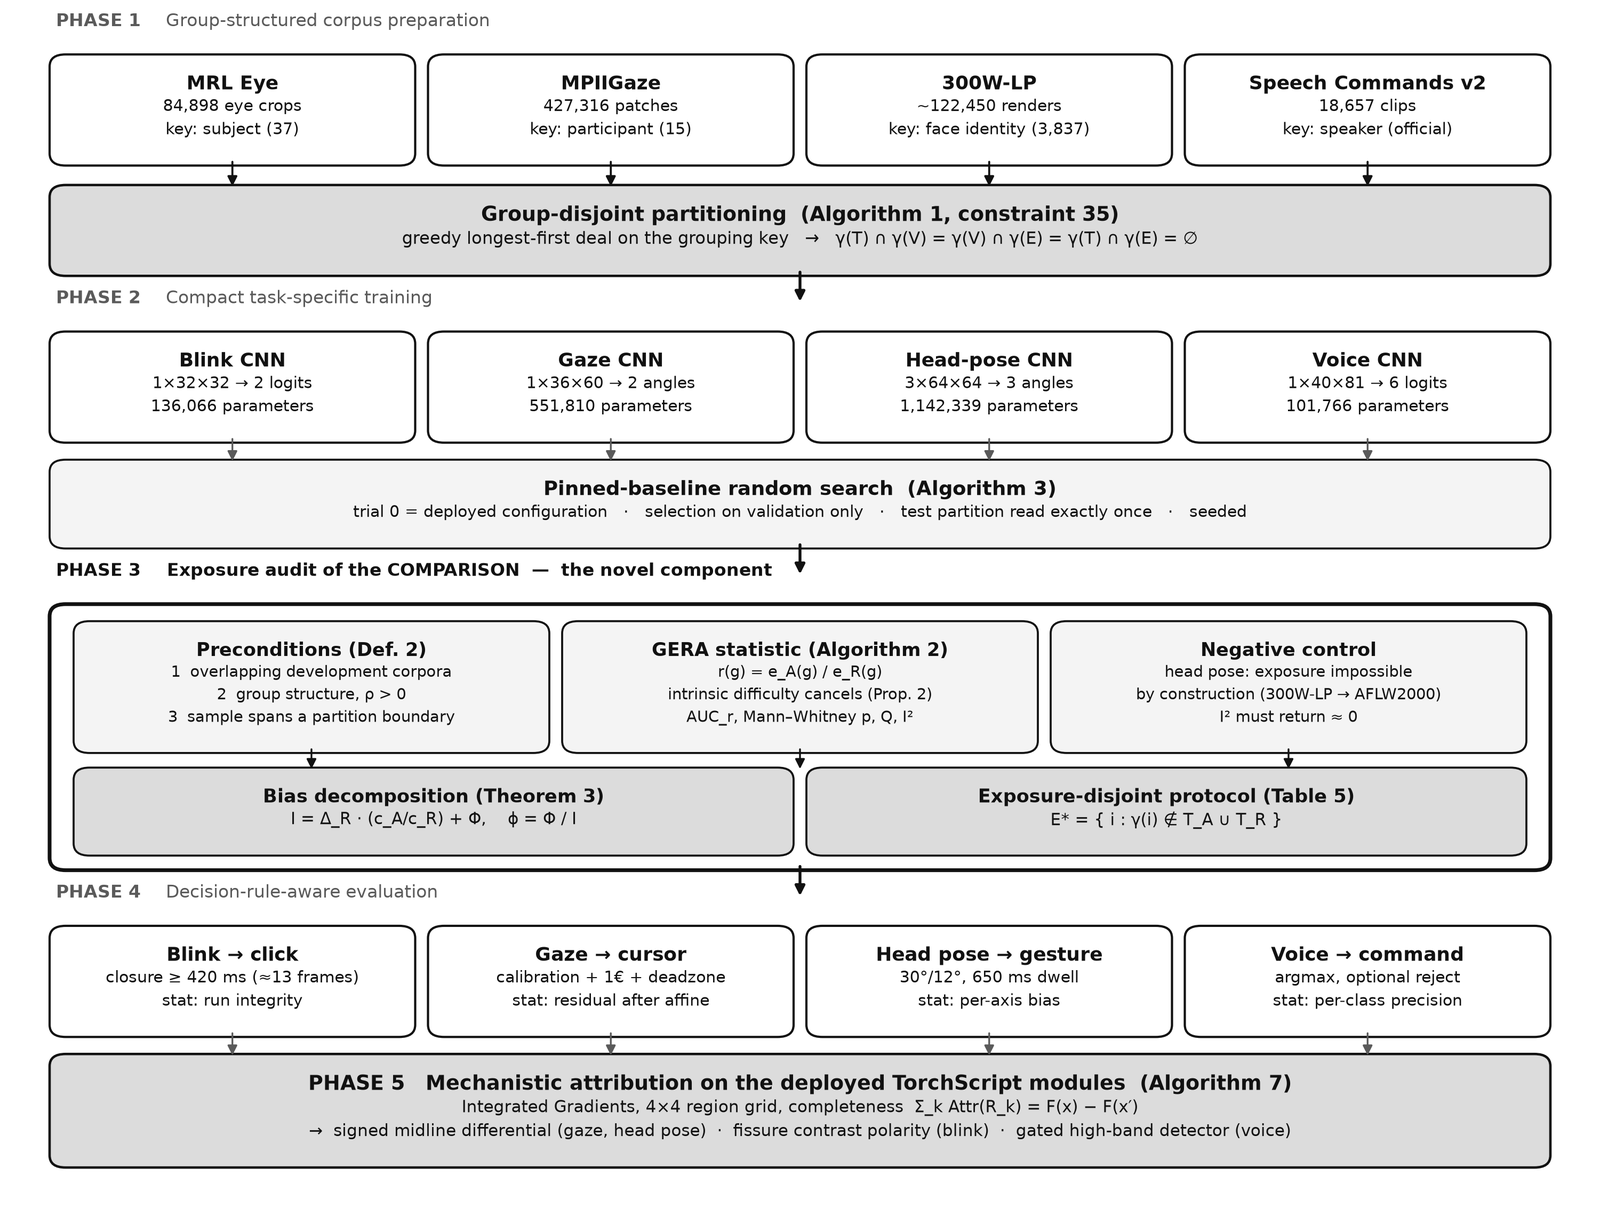
\includegraphics[width=\linewidth]{figures/protocol_P0_framework.png}
\caption{Overview of the MAPLE framework. Four group-structured corpora are partitioned by identity, feeding four compact task-specific networks trained under a pinned-baseline random search. Before any cross-model comparison is reported, the comparison itself is audited for asymmetric exposure by the GERA statistic against a reference model, with a negative control on a corpus where exposure is impossible by construction; only exposure-disjoint strata enter the reported contrast. Each network's error is then read through the deployed decision rule that consumes it, and Integrated-Gradients attribution on the shipped TorchScript modules identifies the operator each network computes.}
\label{fig:1}
\end{figure}

\FloatBarrier

\subsection{Problem formalisation}

\subsubsection{The interaction system as a composition}

Let the system observe, at discrete time \emph{t}, a camera frame \textbf{I}$_{t}$ $\in$ $\mathbb{R}^{(H \times W \times 3)}$ and an audio buffer \textbf{a}$_{t}$ $\in$ $\mathbb{R}^{L}$. A \emph{modality} m $\in$ $\mathcal{M}$ = \{blink, gaze, pose, voice\} is a pair ($f_{m}$, $\Delta_{m}$) consisting of a learned perception map $f_{m}$ and a deterministic decision rule $\Delta_{m}$. Writing $\mathcal{C}_{m}$ for the modality-specific crop or transform applied to the raw observation, the per-frame computation is

\begin{equation}
\label{eq:1}
\begin{aligned}
u_m, _{t} = f_m(\mathcal{C}_m(\mathbf{I}_{t}, \mathbf{a}_{t}) ; \vartheta _m), a_{m}, \\
_{t} = \Delta _m(u_m,_{t}, u_m,_{t-1}, \dots , u_m,_{t-}K ; \psi _m)
\end{aligned}
\end{equation}

where $\vartheta_{m}$ are the learned parameters, $\psi_{m}$ the decision-rule parameters (thresholds, dwell times, hysteresis bands, filter cut-offs), and $a_{m}$,$_{t}$ $\in$ $\mathcal{A}_{m}$ the emitted action, with $\mathcal{A}_{m}$ possibly containing a null action. The essential structural point, and the one that governs the entire evaluation design of Section 3.11, is that the user experiences the composite $\Delta_{m}$ $\circ$ $f_{m}$ and never $f_{m}$ alone. Consequently the loss under which $f_{m}$ is \emph{trained} and the statistic by which $f_{m}$ is \emph{usefully reported} need not coincide, and in three of the four modalities studied here they do not.

The complete system output at time \emph{t} is the arbitrated union

\begin{equation}
\label{eq:2}
\mathcal{S}(\mathbf{I}_{t}, \mathbf{a}_{t}) = \bigcup _{m \in \mathcal{M}} \Delta _m(f_m(\mathcal{C}_m(\mathbf{I}_{t}, \mathbf{a}_{t}))),
\end{equation}

subject to an arbitration relation that suppresses conflicting simultaneous actions (Section 3.9.5).

\subsubsection{The concurrency constraint}

The three vision modalities share a single face-landmark inference \CITE{mediapipe,facemesh} $\ell$(\textbf{I}$_{t}$), executed once per frame, whose output supplies the crops $\mathcal{C}_{\mathrm{blink}}$, $\mathcal{C}_{\mathrm{gaze}}$ and $\mathcal{C}_{\mathrm{pose}}$. Writing $\tau$($\cdot$) for wall-clock latency, real-time operation at frame rate F requires

\begin{equation}
\label{eq:3}
\tau (\ell ) + \Sigma _{m \in \mathcal{M}_{\mathrm{vis}}} [ \tau (\mathcal{C}_m) + \tau (f_m) + \tau (\Delta _m) ] + \tau (\text{stab}) \leq 1 / F
\end{equation}

with $\mathcal{M}_{\mathrm{vis}}$ = \{blink, gaze, pose\} and $\tau$(stab) the cursor stabilisation chain. At F = 30 Hz the budget is 33.3 ms. The voice modality runs on an independent audio thread and enters \EQREF{3} only through CPU contention, not through the frame-serial path. Inequality \EQREF{3} is the constraint that makes the \emph{sum} of model costs the binding quantity, and therefore the constraint under which an individual model's accuracy may rationally be traded.

\subsubsection{Risk, and why the empirical risk is the wrong target here}

For a modality with sample space $\mathcal{X}_{m}$ $\times$ $\mathcal{Y}_{m}$, distribution $\mathcal{D}_{m}$ and loss $\ell_{m}$, the population risk of a hypothesis f is

\begin{equation}
\label{eq:4}
R_m(f) = \mathbb{E}_{(x,y) \sim \mathcal{D}_m} [ \ell _m(f(x), y) ]
\end{equation}

estimated on a finite sample S = \{(x$_{i}$, y$_{i}$)\}$_{i=1}^{n}$ by

\begin{equation}
\label{eq:5}
\hat{R}_m(f ; S) = (1/n) \Sigma _{i=1}^{n} \ell _m(f(x_{i}), y_{i}).
\end{equation}

The estimator \EQREF{5} is unbiased for \EQREF{4} only when the sample is drawn i.i.d. from $\mathcal{D}_{m}$. In every corpus used here it is not: samples are organised into groups (a subject, a participant, a base face identity, a speaker) with strong within-group dependence, and the deployment distribution places the \emph{entire} group of a new user outside the training data. The relevant risk is therefore the group-conditional one,

\begin{equation}
\label{eq:6}
R_m^{\mathrm{grp}}(f) = \mathbb{E}_{g \sim \mathcal{G}} \mathbb{E}_{(x,y) \sim \mathcal{D}_m(\cdot | g)} [ \ell _m(f(x), y) ],
\end{equation}

where $\mathcal{G}$ is the population of groups. Equations \EQREF{5} and \EQREF{6} coincide only if the evaluation groups are disjoint from the training groups; Sections 3.4 and 3.5 are concerned with the two distinct ways in which that condition can fail.

\subsubsection{Notation}

\TABREF{3} fixes the notation used throughout. Modality subscripts are dropped wherever the context is unambiguous.

\begin{table}[pos=htbp]
\centering
\caption{Summary of mathematical notation.}
\label{tab:3}
\footnotesize
\begin{tabularx}{\textwidth}{XX}
\toprule
\textbf{Symbol} & \textbf{Description} \\
\midrule
$\mathcal{M}$, $\mathcal{M}_{\mathrm{vis}}$ & Set of modalities; the three vision modalities sharing one landmark inference \\
$f_{m}$($\cdot$ ; $\vartheta_{m}$) & Learned perception map of modality \emph{m} with parameters $\vartheta_{m}$ \\
$\Delta_{m}$($\cdot$ ; $\psi_{m}$) & Deployed decision rule consuming $f_{m}$, with parameters $\psi_{m}$ \\
$\mathcal{C}_{m}$ & Modality-specific crop / transform of the raw observation \\
$\mathcal{G}$, g & Population of groups; a single group (subject, participant, face identity, speaker) \\
$\gamma$(i) $\in$ $\mathcal{G}$ & Group label of sample \emph{i} \\
$\mathcal{T}_{A}$, $\mathcal{T}_{R}$ & Training-partition group sets of the audited and reference models \\
$\mathcal{V}$, $\mathcal{E}$ & Validation and evaluation index sets \\
A, R & Audited model and reference (control) model \\
$e_{A}$(i), $e_{R}$(i) & Per-sample error of the audited and reference model on sample \emph{i} \\
$\bar{e}_{A}$(g), $\bar{e}_{R}$(g) & Group-mean error of A and R on group \emph{g} \\
r(g) & Group error ratio $\bar{e}_{A}$(g) / $\bar{e}_{R}$(g) --- the GERA statistic \\
d(g) & Intrinsic difficulty of group \emph{g} \\
$c_{A}$, $c_{R}$ & Model-level capability constants \\
$\varphi$ & Familiarity discount enjoyed by a model on its own training groups \\
$\rho$ & Intraclass correlation of the loss within a group \\
n, $n_{g}$, G & Sample count; samples in group \emph{g}; number of groups \\
$n_{\mathrm{eff}}$ & Effective sample size after accounting for within-group dependence \\
$\pi$ & Per-group sampling quota vector of the evaluation sample \\
s & Fitted regression gain of predicted on true target (shrinkage gain) \\
$\theta$, $\hat{\theta }$ & True and predicted target (angle, in radians or degrees) \\
$\sigma^{2}$, $\sigma_{\varepsilon^{2}}$ & Target variance; irreducible representational noise variance \\
Q, I$^{2}$ & Cochran's heterogeneity statistic and the derived inconsistency index \\
$\alpha_{\mathrm{OE}}$, $\beta$, $f_{c}$ & One-euro filter smoothing factor, speed coefficient, cut-off \\
\textbf{w}, \textbf{P}, $\lambda_{f}$ & Calibration weights, RLS inverse-covariance, forgetting factor \\
$T_{\mathrm{hold}}$, $T_{\mathrm{dwell}}$, $T_{\mathrm{cd}}$ & Blink hold threshold, gesture dwell time, cooldown \\
$\theta_{\mathrm{on}}$, $\theta_{\mathrm{off}}$ & Gesture trigger and release thresholds (hysteresis band) \\
$\mathcal{A}_{m}$ & Action alphabet of modality \emph{m} \\
\bottomrule
\end{tabularx}
\end{table}

\FloatBarrier

\subsection{Corpora, grouping keys and evaluation sets}

Four public corpora supply the four modalities. Each is assigned an explicit grouping key, and that assignment is the precondition for everything that follows: a corpus with group structure and within-group dependence is exactly a corpus in which both leakage faults of Section 3.4 and Section 3.5 can occur.

\begin{table}[pos=htbp]
\centering
\caption{Corpora, grouping keys and evaluation sets.}
\label{tab:4}
\footnotesize
\begin{tabularx}{\textwidth}{XXXXXX}
\toprule
\textbf{Modality} & \textbf{Training corpus} & \textbf{Evaluation set} & \textbf{N} & \textbf{Grouping key} & \textbf{Groups} \\
\midrule
Blink & MRL Eye Dataset (84,898 greyscale/IR eye crops) & Held-out subjects & 12,927 & Subject identity & 37 \\
Gaze & MPIIGaze, normalised patches (427,316) & Held-out participants & 64,172 & Participant & 15 \\
Head pose & 300W-LP (\textasciitilde{}122,450 synthesised renders) & AFLW2000, untouched & 1,969 & Base face identity & 3,837 \\
Voice & Speech Commands v2 (18,657 clips, 6 keywords) & Official test list & 2,468 & Speaker & official \\
\bottomrule
\end{tabularx}
\end{table}

\subsubsection{Within-group dependence and effective sample size}

Let $\ell_{i}$ = $\ell$(f(x$_{i}$), y$_{i}$) denote the per-sample loss and let $\gamma$(i) be the group label. Model the loss by a one-way random-effects decomposition

\begin{equation}
\label{eq:7}
\begin{aligned}
\ell _{i} = \mu + b_{\gamma (i)} + \varepsilon _{i}, b_g \sim (0, \sigma _b^{2}), \\
\varepsilon _{i} \sim (0, \sigma _w^{2}),
\end{aligned}
\end{equation}

with b and $\varepsilon$ independent. The intraclass correlation of the loss \CITE{kish} is then

\begin{equation}
\label{eq:8}
\rho = \sigma _b^{2} / (\sigma _b^{2} + \sigma _w^{2}),
\end{equation}

and for a sample containing G groups of equal size $\bar{n}$ = n/G the variance of the sample mean loss is inflated relative to the i.i.d. case by the design effect

\begin{equation}
\label{eq:9}
\begin{aligned}
\mathrm{Var}(\bar{\ell }) = (\sigma _b^{2} + \sigma _w^{2})/n \cdot [ 1 + (\bar{n} - 1) \rho ], \\
\mathrm{DEFF} = 1 + (\bar{n} - 1) \rho ,
\end{aligned}
\end{equation}

so that the effective sample size is

\begin{equation}
\label{eq:10}
n_{\mathrm{eff}} = n / [ 1 + (\bar{n} - 1) \rho ].
\end{equation}

Equation \EQREF{10} is the quantitative statement of why a corpus with thousands of frames per participant does not supply thousands of independent observations, and why the number of \emph{groups} rather than the number of \emph{rows} is the sample size that governs a cross-person claim. For the gaze evaluation of Section 5.2, n = 64,172 rows drawn from G = 2 held-out participants gives $n_{\mathrm{eff}}$ $\to$ 2/$\bar{\rho }$ as $\bar{n}$ grows, which is why Section 6 records the held-out participant count as the principal limitation of the study notwithstanding the large row count.

\subsubsection{The leakage probability under random row splitting}

Consider partitioning n rows uniformly at random into a training fraction p and a test fraction 1 -- p, ignoring group structure. For a test row i belonging to a group of size $n_{g}$, the probability that at least one row of the same group falls in the training partition is

\begin{equation}
\label{eq:11}
\mathbb{P}[ \text{leak}\;(i) ] = 1 - (1 - p)^{n_g - 1} ,
\end{equation}

which for the corpora of \TABREF{4} is numerically indistinguishable from unity: with p = 0.7 and $n_{g}$ = 2,300 (MRL), 1 -- $0.3^{2299}$ < $10^{-1200}$. Under random row splitting essentially \emph{every} test row has a near-duplicate exemplar of the same individual available in training, and the expected fraction of the test set that is contaminated in this sense is

\begin{equation}
\label{eq:12}
\mathbb{E}[ \text{contaminated fraction} ] = (1/n) \Sigma _{i=1}^{n} [ 1 - (1 - p)^{n_{\gamma (i)} - 1} ] \approx 1.
\end{equation}

The measured consequence is reported in Section 5.1: replacing random row splitting by group-disjoint splitting costs 5.81 pp of blink accuracy and 4.11$^{\circ}$ of gaze angular error, while leaving head pose and voice --- whose evaluation sets are group-disjoint by construction --- unchanged to within the seed-to-seed noise floor.

\FloatBarrier

\subsection{Preprocessing and input representations}

Each modality applies a deterministic transform $\mathcal{C}_{m}$ from raw observation to network input. All transforms are implemented identically in the training scripts and in the deployed providers, with the single documented exception noted in Section 5.2.1.

\subsubsection{Eye-region extraction and photometric normalisation (blink)}

Given the landmark set $\mathcal{L}$(\textbf{I}) returned by the shared face-landmark inference, the eye region is the axis-aligned bounding box of the palpebral landmark subset $\mathcal{L}_{\mathrm{eye}}$, expanded by a margin $\kappa$ and resampled to the canonical size 32 $\times$ 32:

\begin{equation}
\label{eq:13}
\mathbf{b} = [ \mathrm{min}_x \mathcal{L}_{\mathrm{eye}} - \kappa w, \mathrm{min}_y \mathcal{L}_{\mathrm{eye}} - \kappa h, \mathrm{max}_x \mathcal{L}_{\mathrm{eye}} + \kappa w, \mathrm{max}_y \mathcal{L}_{\mathrm{eye}} + \kappa h ],
\end{equation}

\begin{equation}
\label{eq:14}
x_{\mathrm{blink}} = \mathrm{Resize}_{32\times 32} ( \mathrm{Gray} ( \mathbf{I} [ \mathbf{b} ] ) ) / 255 \in [0,1]^{32\times 32}.
\end{equation}

Photometric normalisation applies per-crop standardisation, which removes the additive and multiplicative illumination terms that dominate variation across sessions and devices:

\begin{equation}
\label{eq:15}
\begin{aligned}
\tilde{x} = ( x - \mu _x ) / ( \sigma _x + \epsilon ), \\
\mu _x = (1/|x|) \Sigma _{u} x_u, \\
\sigma _x^{2} = (1/|x|) \Sigma _{u} (x_u - \mu _x)^{2},
\end{aligned}
\end{equation}

with $\epsilon$ = 10$^{-6}$ guarding degenerate crops. Section 5.5 shows via attribution that the network subsequently learns a \emph{contrast-polarity} code over the central fissure region, which is precisely the representation for which \EQREF{15} is the correct normalisation, since a polarity code is invariant to the affine photometric family that \EQREF{15} quotients out.

\subsubsection{Gaze patch normalisation and angular parameterisation}

MPIIGaze supplies eye patches already normalised by the standard procedure, which applies a virtual camera rotation \textbf{R}\_n and scaling \textbf{S}\_n such that the eye centre lies on the optical axis at fixed distance and the eye's horizontal axis is image-aligned:

\begin{equation}
\label{eq:16}
\begin{aligned}
\mathbf{M} = \mathbf{S}_n \mathbf{R}_n, \\
x_{\mathrm{gaze}} = \mathrm{Warp}_{\mathbf{M}} ( \mathrm{Gray} ( \mathbf{I} ) ) \in \mathbb{R}^{36\times 60}.
\end{aligned}
\end{equation}

The corpus annotates a 3-D gaze unit vector \textbf{g} = ($g_{x}$, $g_{y}$, $g_{z}$)$^{\mathsf{T}}$ in the normalised camera frame, converted to the pitch--yaw parameterisation the network regresses:

\begin{equation}
\label{eq:17}
\hat{\mathbf{g}} = \mathbf{g} / ( \|\mathbf{g}\|_{2} + \epsilon ),
\end{equation}

\begin{equation}
\label{eq:18}
\begin{aligned}
\theta _{\mathrm{pitch}} = \arcsin( - \hat{g}_y ), \\
\theta _{\mathrm{yaw}} = \arctan2( - \hat{g}_x , - \hat{g}_z ).
\end{aligned}
\end{equation}

The inverse map, used to recover a direction from a prediction for angular-error computation, is

\begin{equation}
\label{eq:19}
\mathbf{g}(\theta _{\mathrm{pitch}}, \theta _{\mathrm{yaw}}) = ( - \cos \theta _{\mathrm{pitch}} \sin \theta _{\mathrm{yaw}} , - \sin \theta _{\mathrm{pitch}} , - \cos \theta _{\mathrm{pitch}} \cos \theta _{\mathrm{yaw}} )^{\mathsf{T}}.
\end{equation}

Angular error between a prediction and ground truth is computed on the sphere rather than in the parameter plane, since the parameter plane is not isometric:

\begin{equation}
\label{eq:20}
e_{\mathrm{ang}} = \arccos ( \mathrm{clip}_{[-1,1]} ( \mathbf{g}(\hat{\theta }) \cdot \mathbf{g}(\theta ) ) ) \cdot 180/\pi [\text{degrees}].
\end{equation}

Equation \EQREF{20} is the statistic reported throughout as ``angular error''; the separately reported ``MAE'' is the mean absolute error in the (pitch, yaw) parameter plane,

\begin{equation}
\label{eq:21}
\mathrm{MAE} = (1/2n) \Sigma _{i=1}^{n} ( |\hat{\theta }_{\mathrm{pitch}},i - \theta _{\mathrm{pitch}},i| + |\hat{\theta }_{\mathrm{yaw}},i - \theta _{\mathrm{yaw}},i| ) \cdot 180/\pi ,
\end{equation}

and the two are reported together because they respond differently to the shrinkage mechanism of Section 5.2.2: \EQREF{20} is a chordal quantity that grows with eccentricity, \EQREF{21} a per-axis quantity that does not.

\subsubsection{Face crop and head-pose parameterisation}

The head-pose network consumes a square RGB crop derived from the 68-point landmark set, expanded to include the full facial envelope:

\begin{equation}
\label{eq:22}
\begin{aligned}
c = ( (\mathrm{min}_x + \mathrm{max}_x)/2 , (\mathrm{min}_y + \mathrm{max}_y)/2 ), \\
\ell _{\mathrm{side}} = (1 + \kappa _f) \cdot \mathrm{max}( \mathrm{max}_x - \mathrm{min}_x , \mathrm{max}_y - \mathrm{min}_y ),
\end{aligned}
\end{equation}

\begin{equation}
\label{eq:23}
x_{\mathrm{pose}} = \mathrm{Resize}_{64\times 64} ( \mathbf{I} [ c \pm \ell _{\mathrm{side}}/2 ] ) \in \mathbb{R}^{3\times 64\times 64}.
\end{equation}

Ground-truth pose is supplied as intrinsic Euler angles (pitch, yaw, roll) = ($\theta_{p}$, $\theta_{y}$, $\theta_{r}$), which define the rotation

\begin{equation}
\label{eq:24}
\mathbf{R} = \mathbf{R}_z(\theta _r) \mathbf{R}_y(\theta _y) \mathbf{R}_x(\theta _p),
\end{equation}

with the usual elementary rotations

\begin{equation}
\label{eq:25}
\begin{aligned}
\mathbf{R}_x(a) = \begin{bmatrix} 1 & 0 & 0 \\ 0 & \cos a & -\sin a \\ 0 & \sin a & \cos a \end{bmatrix}, \\
\mathbf{R}_y(a) = \begin{bmatrix} \cos a & 0 & \sin a \\ 0 & 1 & 0 \\ -\sin a & 0 & \cos a \end{bmatrix}, \\
\mathbf{R}_z(a) = \begin{bmatrix} \cos a & -\sin a & 0 \\ \sin a & \cos a & 0 \\ 0 & 0 & 1 \end{bmatrix}.
\end{aligned}
\end{equation}

The network regresses ($\theta_{y}$, $\theta_{p}$, $\theta_{r}$) in degrees directly. Samples with max(|$\theta_{y}$|, |$\theta_{p}$|, |$\theta_{r}$|) > 99$^{\circ}$ are excluded, following the standard protocol, because beyond that range the projected facial evidence is largely self-occluded and the annotation itself becomes unreliable; Section 5.3 shows that error nevertheless grows sharply well inside this bound and identifies the occlusion mechanism responsible.

Horizontal flip augmentation is \emph{not} label-preserving for this task, and applying it naively is a silent correctness fault. The correct paired transform is

\begin{equation}
\label{eq:26}
( x , (\theta _y, \theta _p, \theta _r) ) \mapsto ( \text{flip}\;_h(x) , (-\theta _y, \theta _p, -\theta _r) ),
\end{equation}

and Section 5.3 reports the diagnostic that confirms it was applied correctly: the per-band error distributions broaden and shift together rather than becoming bimodal, whereas sign confusion from an uncorrected flip would produce bimodality.

\subsubsection{Log-mel acoustic front end}

Audio is resampled to $F_{s}$ = 16 kHz and reduced to a fixed one-second window by right-padding or truncation:

\begin{equation}
\label{eq:27}
a'[n] = a[n] \cdot \mathbf{1}[ n < \mathrm{min}(L, F_s) ] , n = 0, \dots , F_s - 1.
\end{equation}

The short-time Fourier transform \CITE{welch} uses $N_{\mathrm{fft}}$ = 400 (25 ms) with hop H = 200 (12.5 ms), giving T = 81 frames:

\begin{equation}
\label{eq:28}
X[k, \tau ] = \Sigma _{n=0}^{N_{\mathrm{fft}} - 1} a'[ \tau H + n ] \cdot w[n] \cdot \mathrm{exp}( -j 2\pi k n / N_{\mathrm{fft}} ),
\end{equation}

with w a Hann window. The power spectrum is projected onto B = 40 mel-spaced triangular filters,

\begin{equation}
\label{eq:29}
\mathrm{mel}(f) = 2595 \cdot \mathrm{log}_{10}( 1 + f/700 ),
\end{equation}

\begin{equation}
\label{eq:30}
\begin{aligned}
H_b[k] = \mathrm{triangular} \;\text{filter b}, \;\text{centred at} \\ 
\mathrm{mel}^{-1}( \mathrm{mel}(f_{\mathrm{low}}) + b \cdot ( \mathrm{mel}(f_{\mathrm{high}}) - \mathrm{mel}(f_{\mathrm{low}}) ) / (B+1) ),
\end{aligned}
\end{equation}

\begin{equation}
\label{eq:31}
M[b, \tau ] = \Sigma _{k} H_b[k] \cdot | X[k, \tau ] |^{2} ,
\end{equation}

and compressed logarithmically to give the network input

\begin{equation}
\label{eq:32}
\begin{aligned}
x_{\mathrm{voice}}[b, \tau ] = \mathrm{log}( M[b, \tau ] + \epsilon ) , \\
\epsilon = 10^{-6} , x_{\mathrm{voice}} \in \mathbb{R}^{1 \times 40 \times 81}.
\end{aligned}
\end{equation}

The logarithm in \EQREF{32} is what makes the representation approximately invariant to recording gain, since a multiplicative gain becomes an additive offset that the first convolution's bias and the subsequent batch normalisation absorb. Section 5.4 shows via attribution that the network learns an implicit voice-activity gate over the time axis of \EQREF{32} --- concentrating attribution on central time slots and discarding the silence padding --- which is the property that permits transfer to a live microphone stream whose padding statistics differ from the corpus.

\subsubsection{The augmentation operator family}

Augmentation is modelled as a distribution over label-preserving (or label-covariantly-transformed) operators. Writing $\mathcal{A}$ = \{$T_{\omega}$ : $\omega$ $\sim$ $p_{\omega}$\} for the family, training minimises the augmented risk

\begin{equation}
\label{eq:33}
\hat{R}^{\mathrm{aug}}(f ; S) = (1/n) \Sigma _{i=1}^{n} \mathbb{E}_{\omega \sim p_{\omega} } [ \ell ( f(T_{\omega} (x_{i})), \mathcal{T}_{\omega} (y_{i}) ) ] ,
\end{equation}

where $\mathcal{T}_{\omega}$ is the induced label transform --- the identity for blink and voice, the sign flip of \EQREF{26} for head pose, and yaw negation for gaze. The operator family used for the gaze domain-shift correction of Section 5.2.1 is constructed to model the \emph{specific} deterministic shift between normalised training patches and landmark-cropped inference regions, and is therefore analytic rather than generic:

\begin{equation}
\label{eq:34}
\begin{aligned}
T_{\omega} = \mathrm{Rot}(\delta ) \circ \mathrm{Jitter}(\alpha , \beta ) \circ \mathrm{Blur}(\sigma _b) , \\
\delta \sim \mathcal{U}(-8^{\circ}, +8^{\circ}), \alpha \sim \mathcal{U}(0.8, 1.2), \\
\beta \sim \mathcal{U}(-0.2, 0.2), \\
\sigma _b \sim \mathcal{U}(0, \sigma _{\mathrm{max}}),
\end{aligned}
\end{equation}

with Jitter($\alpha$, $\beta$) applying x $\mapsto$ clip($\alpha$ x + $\beta$), Blur($\sigma_{b}$) a Gaussian kernel modelling sensor resolution loss, and Rot($\delta$) an in-plane rotation modelling residual head roll. Because every member of \EQREF{34} is label-preserving up to the flip correction, any gain it produces cannot be additional supervision; it is an enlargement of the effective input manifold at zero parameter and zero data cost. Section 5.2.1 measures a 9.5 \% reduction in \emph{both} a robust and a non-robust error statistic, which is the signature of removing a distributional mismatch rather than repairing isolated failures.

\FloatBarrier

\subsection{First-order leakage: group-disjoint partitioning}

\subsubsection{The partition constraint}

Let the index set be [n] = \{1, $\dots$, n\} with group labels $\gamma$ : [n] $\to$ $\mathcal{G}$. A three-way partition ([n] = $\mathcal{T}$ $\uplus$ $\mathcal{V}$ $\uplus$ $\mathcal{E}$) is \emph{group-disjoint} if

\begin{equation}
\label{eq:35}
\begin{aligned}
\gamma (\mathcal{T}) \cap \gamma (\mathcal{V}) = \emptyset , \\
\gamma (\mathcal{V}) \cap \gamma (\mathcal{E}) = \emptyset , \\
\gamma (\mathcal{T}) \cap \gamma (\mathcal{E}) = \emptyset ,
\end{aligned}
\end{equation}

that is, no group contributes rows to more than one part. Under \EQREF{35} the evaluation estimator \EQREF{5} is an unbiased estimate of the group-conditional risk \EQREF{6} restricted to the evaluation groups, whereas under random row splitting it estimates a mixture that Section 3.5.2 makes explicit.

Because group sizes are highly unequal --- MRL subjects span roughly 700 to 10,000 frames --- a partition that is group-disjoint need not be close to the target row fractions. We therefore deal groups greedily in decreasing size order into whichever part is furthest below its row target, which is the classical longest-processing-time-first heuristic for multiway number partitioning \CITE{graham}:

\begin{equation}
\label{eq:36}
\begin{aligned}
\text{part}\;(g) = \mathrm{arg\,\mathrm{max}}_{j \in {1,2,3}} ( n \cdot \varphi _j - c_j ), \\
c_j \leftarrow c_j + n_g ,
\end{aligned}
\end{equation}

with $\varphi$ = (0.70, 0.15, 0.15) the target fractions and $c_{j}$ the running row count of part \emph{j}. The heuristic admits the standard bound: for group sizes $n_{(1)}$ $\geq$ $n_{(2)}$ $\geq$ $\dots$ the maximum deviation of any part from its target satisfies

\begin{equation}
\label{eq:37}
| c_j - n \varphi _j | \leq \mathrm{max}_g n_g ,
\end{equation}

which is tight in the worst case but far from tight in practice; the realised deviations for all four corpora are below 5 \% of n. \ALGREF{1} states the procedure.

\begin{algorithm}[htbp]
\caption{Group-disjoint partitioning (greedy longest-first deal)}
\label{alg:1}
\hrule\vspace{3pt}
{\ttfamily\scriptsize\raggedright
Require: group labels $\gamma$(1..n); target fractions $\varphi$ = ($\varphi_{1}$, $\varphi_{2}$, $\varphi_{3}$) with $\Sigma \varphi_{j}$ = 1; seed $\sigma$ \\
Ensure: index sets $\mathcal{T}$, $\mathcal{V}$, $\mathcal{E}$ satisfying the disjointness constraint (35) \\
~1: $\mathcal{U}$ $\leftarrow$ unique($\gamma$);~~rng $\leftarrow$ RandomState($\sigma$);~~shuffle($\mathcal{U}$, rng) \\
~2: for all g $\in$ $\mathcal{U}$ do $n_{g}$ $\leftarrow$ |\{ i : $\gamma$(i) = g \}| end for \\
~3: targets $\leftarrow$ (n$\cdot\varphi_{1}$, n$\cdot\varphi_{2}$, n$\cdot\varphi_{3}$);~~counts $\leftarrow$ (0, 0, 0);~~buckets $\leftarrow$ ($\emptyset$, $\emptyset$, $\emptyset$) \\
~4: for all g $\in$ sort($\mathcal{U}$, key = --$n_{g}$) do~~~~~~~~~~~~~~~~~~~~$\triangleright$ largest group first \\
~5:~~~~~j $\leftarrow$ arg $max_{j \in \{1,2,3}$\} ( targets[j] -- counts[j] )~~$\triangleright$ furthest below target \\
~6:~~~~~buckets[j] $\leftarrow$ buckets[j] $\cup$ \{g\};~~counts[j] $\leftarrow$ counts[j] + $n_{g}$ \\
~7: end for \\
~8: $\mathcal{T}$ $\leftarrow$ \{ i : $\gamma$(i) $\in$ buckets[1] \};~~$\mathcal{V}$ $\leftarrow$ \{ i : $\gamma$(i) $\in$ buckets[2] \};~~$\mathcal{E}$ $\leftarrow$ \{ i : $\gamma$(i) $\in$ buckets[3] \} \\
~9: assert $\gamma$($\mathcal{T}$) $\cap$ $\gamma$($\mathcal{V}$) = $\gamma$($\mathcal{V}$) $\cap$ $\gamma$($\mathcal{E}$) = $\gamma$($\mathcal{T}$) $\cap$ $\gamma$($\mathcal{E}$) = $\emptyset$ \\
10: assert $\mathcal{T}$ $\uplus$ $\mathcal{V}$ $\uplus$ $\mathcal{E}$ = [n] \\
11: return $\mathcal{T}$, $\mathcal{V}$, $\mathcal{E}$
\par}
\vspace{3pt}\hrule
\end{algorithm}

The grouping keys are, per corpus: the subject identifier encoded in the MRL filename; the participant identifier p00--p14 for MPIIGaze; the base face identity for 300W-LP, recovered by stripping the synthesised view index and flip tag from the filename so that all renders of one face share a key; and, for Speech Commands, the official validation and testing lists, which are already speaker-aware and therefore require no custom grouping.

\subsubsection{What the correction is worth, and the internal control}

Three quantities are reported per modality throughout this work: the \emph{published} score obtained under the faulty random-row protocol; the \emph{fair baseline}, retraining the original hyperparameters under the corrected protocol; and the \emph{tuned} score under that same corrected protocol. Separating the three is what prevents the protocol effect and the optimisation effect from being conflated, a conflation that would otherwise make it impossible to attribute any reported improvement.

Two of the four modalities have evaluation sets that are group-disjoint by construction and receive no partition change at all --- head pose is evaluated on AFLW2000, disjoint from 300W-LP by design, and voice uses the official speaker-disjoint split --- so either could in principle serve as an \emph{internal negative control} on the correction itself. If group-disjoint partitioning merely depressed scores indiscriminately, an unchanged partition would nonetheless fall along with the changed ones. Section 5.1.1 reports that head pose moves by less than the seed-to-seed noise floor and therefore does serve as that control, which is what licenses attributing the blink and gaze corrections to leakage rather than to a stricter protocol in general; a single-modality study could not supply it. It also reports that the voice figure moves by 7.24 pp despite an unchanged partition, for reasons this study does not establish, and voice is therefore \textbf{not} relied on as a second control. The control rests on head pose alone, and the reader should weigh it accordingly.

\FloatBarrier

\subsection{Second-order leakage: asymmetric exposure between compared models}

After the correction of Section 3.4 every pipeline in this work is group-disjoint and every model's individually reported score is sound. The \emph{comparison} between them is nevertheless still contaminated, because the fault does not live in either pipeline. It lives in the join.

\subsubsection{Formalisation}

\textbf{Definition 1 (Exposure set).} For a model M evaluated on a sample drawn from group population $\mathcal{G}$, the \emph{exposure set} $\mathcal{T}_{M}$ $\subseteq$ $\mathcal{G}$ is the set of groups whose data entered M's training partition. A group g is \emph{exposed} to M if g $\in$ $\mathcal{T}_{M}$.

\textbf{Definition 2 (Asymmetric exposure).} A comparison between models A and R on an evaluation sample $\mathcal{E}$ with group labels $\gamma$($\mathcal{E}$) $\subseteq$ $\mathcal{G}$ is \emph{asymmetrically exposed} when the following three conditions hold simultaneously:

\begin{enumerate}
\item \textbf{(Overlapping development corpora)} A and R were developed on corpora with non-empty intersection at the group level: $\mathcal{T}_{A}$ $\cap$ $\mathcal{T}_{R}$ $\neq$ $\emptyset$ or both derive from a common corpus;
\item \textbf{(Group structure with within-group dependence)} the corpus carries a grouping key with intraclass loss correlation $\rho$ > 0 in the sense of \EQREF{8};
\item \textbf{(Boundary-spanning evaluation sample)} the evaluation sample is drawn from groups on both sides of at least one model's partition boundary: $\gamma$($\mathcal{E}$) $\cap$ $\mathcal{T}_{A}$ $\neq$ $\emptyset$ \textbf{and} $\gamma$($\mathcal{E}$) \textbackslash\{\} $\mathcal{T}_{A}$ $\neq$ $\emptyset$ (or the same with $\mathcal{T}_{R}$).
\end{enumerate}

Condition 3 is the operative one and the one that per-pipeline auditing cannot see: it is a statement about the relation between the evaluation sample and \emph{the other model's} partition, and neither pipeline's own audit has any representation of that partition.

\textbf{Theorem 1 (Mixture representation and quota sensitivity).} Let A be a model with exposure set $\mathcal{T}_{A}$, and let the evaluation sample allocate a fraction $\pi_{g}$ of its mass to group g, with $\Sigma_{g}$ $\pi_{g}$ = 1. Define the exposed mass

\begin{equation}
\label{eq:38}
\Pi = \Sigma _{g \in \gamma (\mathcal{E}) \cap \mathcal{T}_A} \pi _g \in (0, 1).
\end{equation}

Then the reported aggregate error of A decomposes as the convex combination

\begin{equation}
\label{eq:39}
\bar{E}_A(\pi ) = \Pi \cdot \bar{E}_A^{\mathrm{in}} + (1 - \Pi ) \cdot \bar{E}_A^{\mathrm{out}},
\end{equation}

where $\bar{E}_{A}^{\mathrm{in}}$ and $\bar{E}_{A}^{\mathrm{out}}$ are the exposed- and unexposed-stratum means, each formed by averaging $\bar{e}_{A}$(g) over the groups of its own stratum under the weights $\pi_{g}$ renormalised to sum to one. Consequently

\begin{equation}
\label{eq:40}
\partial \bar{E}_A / \partial \Pi = \bar{E}_A^{\mathrm{in}} - \bar{E}_A^{\mathrm{out}} ,
\end{equation}

and whenever $\bar{E}_{A}^{\mathrm{in}}$ $\neq$ $\bar{E}_{A}^{\mathrm{out}}$ the reported error is a strictly monotone function of the sampling quota $\Pi$ alone. In particular, a change to the per-group sampling quota changes the reported accuracy without changing any model, any datum, or any metric definition.

\emph{Proof.} Write the sample mean error as a group-weighted mean, $\bar{e}_{A}$ = $\Sigma_{g}$ $\pi_{g}$ $\bar{e}_{A}$(g). Split the index set of groups by membership in $\mathcal{T}_{A}$ and factor the exposed mass $\Pi$ out of the first sum and (1 -- $\Pi$) out of the second; this yields \EQREF{39} directly, since the renormalised weights within each stratum sum to one by construction. Differentiating \EQREF{39} in $\Pi$, holding the two conditional means fixed, gives \EQREF{40}. Monotonicity is immediate from the sign of \EQREF{40}. $\blacksquare$

Theorem 1 states precisely what is objectionable. Under Definition 2 the aggregate is a mixture of a \emph{memorisation} regime and a \emph{generalisation} regime, with the mixing weight fixed by a sampling decision rather than by the research question. Two honest evaluators applying the same metric to the same models on the same corpus can report different numbers, and neither is making an error in the ordinary sense.

\textbf{Corollary 1 (Bias of the reported contrast).} Let the quantity of interest be the true cross-group contrast $\Delta$* = $\bar{E}_{A}^{\mathrm{out}}$ -- $\bar{E}_{R}^{\mathrm{out}}$, and let the reported contrast be $\hat{\Delta }$ = $\bar{E}_{A}$($\pi$) -- $\bar{E}_{R}$($\pi$). If R has no differential familiarity across $\gamma$($\mathcal{E}$) --- that is, $\bar{E}_{R}^{\mathrm{in}}$ = $\bar{E}_{R}^{\mathrm{out}}$ --- then

\begin{equation}
\label{eq:41}
\hat{\Delta } - \Delta * = \Pi \cdot ( \bar{E}_A^{\mathrm{in}} - \bar{E}_A^{\mathrm{out}} ) \leq 0,
\end{equation}

so the reported contrast understates A's true disadvantage by exactly the exposed mass times the within-model familiarity gap. The bias is signed, and it always favours the exposed model.

\emph{Proof.} Substitute \EQREF{39} for both models into $\hat{\Delta }$, apply $\bar{E}_{R}^{\mathrm{in}}$ = $\bar{E}_{R}^{\mathrm{out}}$ so that $\bar{E}_{R}$($\pi$) = $\bar{E}_{R}^{\mathrm{out}}$, and subtract $\Delta$*. The sign follows from $\bar{E}_{A}^{\mathrm{in}}$ $\leq$ $\bar{E}_{A}^{\mathrm{out}}$, which holds whenever training exposure does not increase error. $\blacksquare$

Corollary 1 is the reason Section 5 reports every comparison on the exposure-disjoint stratum only, and the reason a baseline trained on the whole corpus must be reported as a \emph{lower bound} on its own cross-person error rather than as a point estimate (protocol step 5, Section 3.5.6).

\subsubsection{The GERA statistic}

An auditor examining a published comparison rarely knows how either model was partitioned. The detector proposed here requires only what such an audit does have: the two prediction streams over a shared evaluation set, and a group label per sample.

\textbf{Definition 3 (Group error ratio).} For each group g $\in$ $\gamma$($\mathcal{E}$), let

\begin{equation}
\label{eq:42}
\begin{aligned}
\bar{e}_A(g) = (1/n_g) \Sigma _{i : \gamma (i) = g} e_A(i), \\
\bar{e}_R(g) = (1/n_g) \Sigma _{i : \gamma (i) = g} e_R(i),
\end{aligned}
\end{equation}

and define the \textbf{group error ratio}

\begin{equation}
\label{eq:43}
r(g) = \bar{e}_A(g) / \bar{e}_R(g).
\end{equation}

The role of R is to calibrate intrinsic group difficulty. Some groups are simply harder than others --- a fact A's own errors cannot separate from familiarity --- and a reference model with no \emph{differential} familiarity across those groups supplies exactly that missing control, because its across-group variation is intrinsic difficulty alone.

\textbf{Proposition 2 (Exact cancellation of intrinsic difficulty).} Suppose per-group errors follow the multiplicative difficulty model

\begin{equation}
\label{eq:44}
\begin{aligned}
\bar{e}_M(g) = d(g) \cdot c_M \cdot ( 1 - \varphi _M \cdot \mathbf{1}[ g \in \mathcal{T}_M ] ) , \\
M \in {A, R},
\end{aligned}
\end{equation}

with d(g) > 0 the intrinsic difficulty of group g, $c_{M}$ > 0 a model-level capability constant, and $\varphi_{M}$ $\in$ [0,1) the familiarity discount M enjoys on its own training groups. Then

\begin{equation}
\label{eq:45}
r(g) = ( c_A / c_R ) \cdot ( 1 - \varphi _A \mathbf{1}[ g \in \mathcal{T}_A ] ) / ( 1 - \varphi _R \mathbf{1}[ g \in \mathcal{T}_R ] ),
\end{equation}

which is free of d(g). If in addition R has no differential familiarity across $\gamma$($\mathcal{E}$) --- either $\mathcal{T}_{R}$ $\supseteq$ $\gamma$($\mathcal{E}$) or $\mathcal{T}_{R}$ $\cap$ $\gamma$($\mathcal{E}$) = $\emptyset$, so the indicator is constant --- then

\begin{equation}
\label{eq:46}
\begin{aligned}
r(g) = \kappa \cdot ( 1 - \varphi _A \mathbf{1}[ g \in \mathcal{T}_A ] ), \\
\kappa = ( c_A / c_R ) / ( 1 - \varphi _R \mathbf{1}[\gamma (\mathcal{E}) \subseteq \mathcal{T}_R] ) ,
\end{aligned}
\end{equation}

so r(g) takes exactly two values, $\kappa$(1 -- $\varphi_{A}$) on exposed groups and $\kappa$ on unexposed groups, and the ratio of the two group means identifies the familiarity discount:

\begin{equation}
\label{eq:47}
\hat{\varphi }_A = 1 - ( \mathrm{mean}_{g \in \mathcal{T}_A} r(g) ) / ( \mathrm{mean}_{g \notin \mathcal{T}_A} r(g) ).
\end{equation}

\emph{Proof.} Substituting \EQREF{44} into \EQREF{43}, the factor d(g) appears in numerator and denominator and cancels identically for every g, giving \EQREF{45}. Under the stated condition on $\mathcal{T}_{R}$ the denominator indicator is constant over $\gamma$($\mathcal{E}$) and may be absorbed into $\kappa$, giving \EQREF{46}. Equation \EQREF{47} follows by taking means over the two strata and forming the ratio. $\blacksquare$

Proposition 2 is the formal content of the phrase ``the reference prices the intrinsic difficulty''. It also states the detector's precondition sharply: R must have \emph{constant} exposure across the evaluation groups. If R is differentially familiar --- exposed to some evaluation groups and not others --- its across-group variation no longer isolates intrinsic difficulty and \EQREF{45} does not reduce.

In practice \EQREF{44} holds only approximately, so r(g) is dispersed rather than two-valued, and the detector is a \emph{screening} statistic. We assess separation by the rank statistic

\begin{equation}
\label{eq:48}
\mathrm{AUC}_r = \mathbb{P}[ r(G_{\mathrm{out}}) > r(G_{\mathrm{in}}) ] = (1/(n_{\mathrm{in}} n_{\mathrm{out}})) \Sigma _{g \in \mathcal{T}_A} \Sigma _{h \notin \mathcal{T}_A} \mathbf{1}[ r(h) > r(g) ] + \tfrac{1}{2} \mathbf{1}[ r(h) = r(g) ],
\end{equation}

with the Mann--Whitney U statistic \CITE{mannwhitney} U = $n_{\mathrm{in}}$ $n_{\mathrm{out}}$ $AUC_{r}$ and the exact two-sided permutation p-value

\begin{equation}
\label{eq:49}
\begin{aligned}
p = \mathbb{P}_{H_{0}}[ | U - \mathbb{E}U | \geq | u_{\mathrm{obs}} - \mathbb{E}U | ], \\
\mathbb{E}U = n_{\mathrm{in}} n_{\mathrm{out}} / 2,
\end{aligned}
\end{equation}

evaluated by enumeration when the group counts are small, as they are here. Confidence on $AUC_{r}$ uses the Hanley--McNeil variance estimate \CITE{hanley}

\begin{equation}
\label{eq:50}
\begin{aligned}
\mathrm{Var}(\mathrm{AUC}_r) = [ \mathrm{AUC}(1-\mathrm{AUC}) + (n_{\mathrm{in}} - 1)(Q_{1} - \mathrm{AUC}^{2}) + (n_{\mathrm{out}} - 1)(Q_{2} - \mathrm{AUC}^{2}) ] \\ 
/ ( n_{\mathrm{in}} n_{\mathrm{out}} ),
\end{aligned}
\end{equation}

with Q$_{1}$ = AUC/(2 -- AUC) and Q$_{2}$ = 2AUC$^{2}$/(1 + AUC).

\subsubsection{Heterogeneity testing and the negative control}

A detector is only as good as its behaviour when there is nothing to detect. We therefore test whether r(g) is \emph{homogeneous} across groups, using the standard random-effects machinery. Let v(g) denote the bootstrap variance \CITE{efron} of r(g), obtained by resampling within group g,

\begin{equation}
\label{eq:51}
\begin{aligned}
v(g) = \mathrm{Var}_{b=1..B} [ r^{(b)}(g) ], \\
r^{(b)}(g) = \bar{e}_A^{(b)}(g) / \bar{e}_R^{(b)}(g),
\end{aligned}
\end{equation}

and let w(g) = 1/v(g) be the inverse-variance weight. The pooled estimate and Cochran's heterogeneity statistic \CITE{cochran} are

\begin{equation}
\label{eq:52}
\bar{r} = \Sigma _g w(g) r(g) / \Sigma _g w(g),
\end{equation}

\begin{equation}
\label{eq:53}
\begin{aligned}
Q = \Sigma _g w(g) ( r(g) - \bar{r} )^{2} , \\
Q \sim \chi ^{2}_{G-1} \;\text{under H}\;_{0} : r(g) \equiv \bar{r} ,
\end{aligned}
\end{equation}

with the derived inconsistency index \CITE{higgins}

\begin{equation}
\label{eq:54}
I^{2} = \mathrm{max}( 0 , ( Q - (G - 1) ) / Q ) \cdot 100 \%.
\end{equation}

I$^{2}$ is the proportion of observed dispersion in r not explained by within-group sampling error. Under the null of no differential familiarity, and with a reference satisfying Proposition 2's condition, r(g) should be homogeneous and I$^{2}$ $\approx$ 0.

The negative control exploits a structural property of the head-pose corpora and costs nothing: both the proposed network and the pretrained baseline train on 300W-LP and are scored on AFLW2000, so neither has seen the evaluation groups, and r(g) must be homogeneous under \emph{any} grouping of the evaluation set. It is a demanding control rather than a trivial one, because intrinsic difficulty varies roughly fourfold across the pose manifold (Section 5.3); if the reference failed to price that variation out, r would track it and the detector would fire on a corpus where no leakage exists. Section 5.1.3 reports the outcome.

One calibration caveat follows from the same machinery and bears on how \EQREF{53}--\EQREF{54} should be read. Cochran's Q is sensitive to sample size: at large $n_{g}$ a negligible effect reaches nominal significance, because w(g) $\propto$ 1/v(g) grows linearly in $n_{g}$ while the null dispersion does not. Formally, for a fixed true dispersion $\delta^{2}$ = $Var_{g}$[r(g)] in excess of sampling error,

\begin{equation}
\label{eq:55}
\mathbb{E}[Q] \approx (G - 1) + \delta ^{2} \Sigma _g w(g) = (G - 1) + O( \delta ^{2} \cdot n ),
\end{equation}

so Q $\to$ $\infty$ with n for any $\delta$ > 0. The \emph{magnitude} of the spread, not its p-value, is therefore the informative readout, and Section 5.1.3 reports a random-grouping control demonstrating exactly this failure of the p-value.

\subsubsection{Decomposing the inflation: difficulty against familiarity}

That an aggregate understates a model's error is an observation; attributing it is a separate step, and the same reference model performs it.

\textbf{Theorem 3 (Exposure-bias decomposition).} Let $\bar{E}_{A}^{\mathrm{all}}$ denote A's error aggregated over all evaluation groups and $\bar{E}_{A}^{\mathrm{out}}$ its error on the unexposed stratum. Define the total inflation

\begin{equation}
\label{eq:56}
\mathrm{I} = \bar{E}_A^{\mathrm{out}} - \bar{E}_A^{\;\text{all}\;} \geq 0.
\end{equation}

Let R be a reference satisfying the condition of Proposition 2, and let

\begin{equation}
\label{eq:57}
\Delta _R = \bar{E}_R^{\mathrm{out}} - \bar{E}_R^{\;\text{all}\;}
\end{equation}

be R's corresponding shift across the identical strata. Then $\mathrm{I}$ admits the decomposition

\begin{equation}
\label{eq:58}
\begin{aligned}
\mathrm{I} = \kappa \cdot \Delta _R + \Phi , \\
\Phi = \mathrm{I} - \kappa \cdot \Delta _R, \phi = \Phi / \mathrm{I} ,
\end{aligned}
\end{equation}

in which $\kappa$ $\cdot$ $\Delta_{R}$ is the \emph{intrinsic-difficulty component} --- the amount by which the unexposed stratum is harder for any model --- $\Phi$ is the \emph{familiarity component} attributable to asymmetric exposure, and $\phi$ is the familiarity fraction. The transfer coefficient $\kappa$ converts a difficulty shift measured in R's error units into A's, and \textbf{its value is not identified by the data; it is fixed by the difficulty model one adopts}:

\begin{equation}
\label{eq:59}
\begin{aligned}
\kappa = 1 (\text{additive difficulty}), \\
\kappa = c_A / c_R (\text{multiplicative difficulty}, as in (44)).
\end{aligned}
\end{equation}

\emph{Proof.} R has no differential familiarity, so by construction the whole of $\Delta_{R}$ is intrinsic difficulty measured in R's error units. Under the additive model $\bar{e}_{M}$(g) = d(g) + $c_{M}$ -- $\varphi_{M}\mathbf{1}$[$\cdot$], a difficulty shift transfers between models unchanged, so $\kappa$ = 1. Under the multiplicative model \EQREF{44} a shift scales with the model's capability constant, so $\kappa$ = $c_{A}$/$c_{R}$. In either case the residual $\Phi$ is by definition the part of $\mathrm{I}$ that difficulty does not explain. $\blacksquare$

Two consequences must be stated with the theorem, because the choice of $\kappa$ is consequential and is a genuine limitation of the instrument rather than a presentational detail.

First, \textbf{$\kappa$ = 1 is the least conservative reading, not the most.} Since $\Phi$ decreases in $\kappa$ and $c_{A}$/$c_{R}$ $\geq$ 1 whenever A is the weaker model, the additive reading \emph{maximises} the familiarity attribution. An auditor who wants a lower bound on $\Phi$ should use the multiplicative reading.

Second, \textbf{the two readings should therefore be reported as an interval} rather than a point estimate. Writing $\kappa_{\mathrm{max}}$ = $c_{A}$/$c_{R}$,

\begin{equation}
\label{eq:60}
\begin{aligned}
\Phi \in [ \mathrm{I} - \kappa _{\mathrm{max}} \Delta _R , \mathrm{I} - \Delta _R ] , \\
\phi \in [ 1 - \kappa _{\mathrm{max}} \Delta _R/\mathrm{I} , 1 - \Delta _R/\mathrm{I} ] .
\end{aligned}
\end{equation}

Section 5.1.2 reports $\mathrm{I}$ = 1.905$^{\circ}$, $\Delta_{R}$ = 0.837$^{\circ}$ and $\kappa_{\mathrm{max}}$ = 1.769 for the affected modality, giving $\Phi$ $\in$ [0.425$^{\circ}$, 1.068$^{\circ}$] and $\phi$ $\in$ [22 \%, 56 \%]. The interval is wide, and no claim in this paper rests on its upper end. What survives the whole of it is the qualitative statement that answers the natural sceptical objection --- that the held-out groups were simply harder --- quantitatively rather than rhetorically: harder they were, but under neither difficulty model does difficulty account for all of the observed gap, and a familiarity component of at least 0.425$^{\circ}$ remains. This is a quantity lineage analysis cannot supply at all, since knowing \emph{that} a model saw a corpus does not say how much of its advantage came from having seen it.

\ALGREF{2} states the complete audit.

\begin{algorithm}[htbp]
\caption{GERA: Group Error-Ratio Audit for asymmetric exposure}
\label{alg:2}
\hrule\vspace{3pt}
{\ttfamily\scriptsize\raggedright
Require: per-sample errors $e_{A}$(i), $e_{R}$(i) over a shared evaluation set $\mathcal{E}$; group labels $\gamma$(i); \\
~~~~~~~~~optional membership labels $\mathbf{1}$[g $\in$ $\mathcal{T}_{A}$]; bootstrap replicates B; control grouping $\gamma_{\mathrm{ctl}}$ \\
Ensure: ratio profile r($\cdot$), separation $AUC_{r}$ and p, heterogeneity (Q, I$^{2}$), decomposition ($\mathrm{I}$, $\Delta_{R}$, $\Phi$, $\phi$) \\
~1: // Phase 1: per-group ratio profile (Definition 3) \\
~2: for all g $\in$ unique($\gamma$) do \\
~3:~~~~~$\bar{e}_{A}$(g) $\leftarrow$ mean\{ $e_{A}$(i) : $\gamma$(i) = g \};~~$\bar{e}_{R}$(g) $\leftarrow$ mean\{ $e_{R}$(i) : $\gamma$(i) = g \} \\
~4:~~~~~r(g) $\leftarrow$ $\bar{e}_{A}$(g) / $\bar{e}_{R}$(g) \\
~5: end for \\
~6: // Phase 2: separation, only if membership labels are available \\
~7: if membership labels available then \\
~8:~~~~~$AUC_{r}$ $\leftarrow$ Mann--Whitney statistic of \{ r(g) : g $\notin$ $\mathcal{T}_{A}$ \} against \{ r(g) : g $\in$ $\mathcal{T}_{A}$ \}~~~$\triangleright$ Eq. (48) \\
~9:~~~~~p $\leftarrow$ exact two-sided permutation p-value~~~~~~~~~~~~~~~~~~~~~~~~~~~~~~~~~~~~~~~~~~~~$\triangleright$ Eq. (49) \\
10:~~~~~CI $\leftarrow$ Hanley--McNeil interval on $AUC_{r}$~~~~~~~~~~~~~~~~~~~~~~~~~~~~~~~~~~~~~~~~~~~~~~~$\triangleright$ Eq. (50) \\
11:~~~~~$\hat{\varphi }_{A}$ $\leftarrow$ 1 -- $mean_{g \in \mathcal{T}_{A}}$ r(g) / $mean_{g \notin \mathcal{T}_{A}}$ r(g)~~~~~~~~~~~~~~~~~~~~~~~~~~~~~~~~$\triangleright$ Eq. (47) \\
12: end if \\
13: // Phase 3: heterogeneity, computable with no membership labels at all \\
14: for all g do v(g) $\leftarrow$ bootstrap variance of r(g) over B within-group resamples end for~~$\triangleright$ Eq. (51) \\
15: w(g) $\leftarrow$ 1 / v(g);~~$\bar{r}$ $\leftarrow$ $\Sigma$ w(g) r(g) / $\Sigma$ w(g)~~~~~~~~~~~~~~~~~~~~~~~~~~~~~~~~~~~~~~~~~~~~$\triangleright$ Eq. (52) \\
16: Q $\leftarrow$ $\Sigma_{g}$ w(g) ( r(g) -- $\bar{r}$ )$^{2}$;~~I$^{2}$ $\leftarrow$ max(0, (Q -- (G--1))/Q)~~~~~~~~~~~~~~~~~~~~~~~~~~~~~~~$\triangleright$ Eqs. (53)--(54) \\
17: spread $\leftarrow$ $max_{g}$ r(g) / $min_{g}$ r(g)~~~~~~~~~~~~~~~~~~~~~~~~$\triangleright$ report magnitude, not p (Eq. 55) \\
18: // Phase 4: negative control on a grouping where exposure is impossible \\
19: repeat lines 2--17 with $\gamma$ $\leftarrow$ $\gamma_{\mathrm{ctl}}$;~~record ($Q_{\mathrm{ctl}}$, I$^{2}_{\mathrm{ctl}}$, $spread_{\mathrm{ctl}}$) \\
20: // Phase 5: bias decomposition against the reference~~~~~~~~~~~~~~~~~~~~~~~~~~~~~~~~~~~$\triangleright$ Theorem 3 \\
21: $\mathrm{I}$ $\leftarrow$ $\bar{E}_{A}^{\mathrm{out}}$ -- $\bar{E}_{A}^{\mathrm{all}}$;~~$\Delta_{R}$ $\leftarrow$ $\bar{E}_{R}^{\mathrm{out}}$ -- $\bar{E}_{R}^{\mathrm{all}}$ \\
22: $\Phi$ $\leftarrow$ $\mathrm{I}$ -- $\Delta_{R}$ $\cdot$ ($c_{A}$/$c_{R}$);~~$\phi$ $\leftarrow$ $\Phi$ / $\mathrm{I}$ \\
23: return r($\cdot$), $AUC_{r}$, p, CI, (Q, I$^{2}$, spread), ($Q_{\mathrm{ctl}}$, I$^{2}_{\mathrm{ctl}}$, $spread_{\mathrm{ctl}}$), ($\mathrm{I}$, $\Delta_{R}$, $\Phi$, $\phi$)
\par}
\vspace{3pt}\hrule
\end{algorithm}

\subsubsection{Scope, and what the detector does not claim}

Three limitations are structural rather than incidental and are stated with the method rather than deferred.

\emph{The statistic is a screening instrument.} Separation is strong but imperfect --- Section 5.1.3 reports one training group sitting at r = 2.18, well inside the unexposed range --- so a single group's ratio must never be treated as proof of membership. The appropriate use is to convert an unfalsifiable suspicion into a testable one at zero additional experimental cost, and then to run the stratified decomposition of Theorem 3, which is the substantive analysis.

\emph{A suitable reference must exist.} If every available model shares the audited model's partition, or if the candidate reference is itself differentially familiar across the evaluation groups, then by Proposition 2 the cancellation fails and r(g) confounds difficulty with familiarity. The near-flatness of a candidate reference's own profile is weak evidence in favour of its admissibility, but it is not a proof, since a reference exposed to \emph{all} groups and a reference exposed to \emph{none} both produce flat profiles.

\emph{No false-positive guarantee is offered.} Unlike black-box contamination proofs \CITE{oren} which yield a formal false-positive bound under an exchangeability assumption, GERA offers no such guarantee. Its value lies in the access regime it operates under: it needs neither model's training data, neither model's lineage documentation, and no corpus access --- only the two prediction streams and the group labels, which are artefacts an external auditor already possesses.

\subsubsection{The exposure-disjoint comparison protocol (EDCP)}

\TABREF{5} states the procedure applied throughout the remainder of this work. Steps 1--2 are established practice \CITE{kapoor,leakage}. Steps 3--5 formalise, for group-structured corpora, the discipline that lineage analysis prescribes informally \CITE{tsfm}, and step 6 adds the prediction-only audit developed above.

\begin{table}[pos=htbp]
\centering
\caption{The exposure-disjoint comparison protocol, and the fault each step addresses.}
\label{tab:5}
\footnotesize
\begin{tabularx}{\textwidth}{cXXX}
\toprule
\textbf{\#} & \textbf{Step} & \textbf{Addresses} & \textbf{Formal object} \\
\midrule
1 & Establish an explicit grouping key for every corpus & Precondition 2 of Definition 2 & $\gamma$ : [n] $\to$ $\mathcal{G}$ \\
2 & Partition group-disjointly within each model's own pipeline & First-order leakage & Constraint \EQREF{35}, \ALGREF{1} \\
3 & Intersect the evaluation sample with \emph{every} compared model's training partition, not only the audited model's & Precondition 3 of Definition 2 & $\gamma$($\mathcal{E}$) $\cap$ $\mathcal{T}_{M}$ for all M \\
4 & Restrict the comparison stratum to groups outside every compared model's training partition & Asymmetric exposure & $\mathcal{E}$* = \{ i : $\gamma$(i) $\notin$ $\bigcup_{M}$ $\mathcal{T}_{M}$ \} \\
5 & Where step 4 is impossible because a baseline trained on the whole corpus, report that baseline's figure as a \textbf{lower bound} and state the direction of the residual bias & Residual bias & Corollary 1, sign of \EQREF{41} \\
6 & Audit the residual with the per-group ratio r(g) against a reference model & Undocumented splits & \ALGREF{2} \\
\bottomrule
\end{tabularx}
\end{table}

Step 5 is not a formality in the present study. The near-flatness of the pretrained gaze baseline's per-group profile (Section 5.1.3) is itself diagnostic of its having trained on all fifteen MPIIGaze participants, so its held-out figure is a lower bound on its true cross-person error. Every comparison in this work is therefore \emph{conservative with respect to the proposed networks} rather than favourable to them --- a point worth stating plainly, because the comparison ends unfavourably for one modality and the reader is entitled to know that the bias runs the other way.

Formally, writing $\bar{E}_{R}^{\mathrm{LB}}$ for the reported baseline figure and $\bar{E}_{R}^{\mathrm{true}}$ for its unobserved cross-person error, step 5 asserts

\begin{equation}
\label{eq:61}
\bar{E}_R^{\mathrm{true}} \geq \bar{E}_R^{\mathrm{LB}} \implies \hat{\Delta } = \bar{E}_A - \bar{E}_R^{\mathrm{LB}} \geq \bar{E}_A - \bar{E}_R^{\mathrm{true}} = \Delta *,
\end{equation}

so the reported contrast $\hat{\Delta }$ overstates rather than understates the proposed network's disadvantage only in the direction that could reverse a favourable conclusion, never one that could manufacture one.

Applying steps 3--4, all gaze results in Section 5 use the two held-out participants only. A 2,000-eye-per-participant cap inherited from the pretrained evaluation initially restricted the comparison to 4,000 samples; both networks were re-run over the full 64,172. We note that the established protocol for person-independent evaluation on MPIIGaze is leave-one-person-out over all fifteen participants \CITE{mpiigaze_pami}; the single group-disjoint split used here is weaker, and Section 6 records this as a limitation of the present \emph{study} rather than of the protocol in \TABREF{5}, which is agnostic to how many folds are run.

\FloatBarrier

\subsection{Network architectures}

All four networks are defined from scratch rather than fine-tuned from an off-the-shelf backbone, for two reasons that are methodological rather than aesthetic. First, a fine-tuned backbone imports an undocumented exposure set from its pretraining corpus, which by Definition 2 is precisely the condition that makes a downstream comparison asymmetrically exposed; training from scratch on a corpus with a known grouping key keeps $\mathcal{T}_{A}$ explicit. Second, the concurrency constraint \EQREF{3} admits parameter budgets two to three orders of magnitude below standard backbones, so the relevant design space is not reachable by pruning a large network.

\subsubsection{Common operators}

Each network is a composition of a convolutional feature extractor and a fully connected head. Write the two-dimensional convolution with kernel \textbf{K} $\in$ $\mathbb{R}^{($C_{\mathrm{out}}$ \times $C_{\mathrm{in}}$ \times k \times k)}$, bias \textbf{b}, stride 1 and padding p = (k--1)/2 as

\begin{equation}
\label{eq:62}
( \mathrm{Conv}_{\mathbf{K},\mathbf{b}}(x) )_{c,u,v} = b_c + \Sigma _{c'=1}^{C_{\mathrm{in}}} \Sigma _{i=1}^{k} \Sigma _{j=1}^{k} K_{c,c',i,j} \cdot x_{c', u+i-p-1, v+j-p-1},
\end{equation}

the rectifier and max-pooling as

\begin{equation}
\label{eq:63}
\begin{aligned}
\mathrm{ReLU}(z) = \mathrm{max}(0, z), \\
( \mathrm{MaxPool}_2(x) )_{c,u,v} = \mathrm{max}_{(i,j) \in {0,1}^{2}} x_{c, 2u+i, 2v+j},
\end{aligned}
\end{equation}

batch normalisation \CITE{batchnorm} over a minibatch $\mathcal{B}$ as

\begin{equation}
\label{eq:64}
\begin{aligned}
\mathrm{BN}_{\gamma ,\beta }(z) = \gamma \cdot ( z - \mu _{\mathcal{B}} ) / \sqrt{\sigma _{\mathcal{B}}^{2} + \epsilon} + \beta , \\
\mu _{\mathcal{B}} = \mathbb{E}_{\mathcal{B}}[z], \\
\sigma _{\mathcal{B}}^{2} = \mathrm{Var}_{\mathcal{B}}[z],
\end{aligned}
\end{equation}

adaptive average pooling to unit spatial extent as

\begin{equation}
\label{eq:65}
( \mathrm{GAP}(x) )_c = (1/(HW)) \Sigma _{u=1}^{H} \Sigma _{v=1}^{W} x_{c,u,v},
\end{equation}

inverted dropout \CITE{dropout} at rate q as

\begin{equation}
\label{eq:66}
\mathrm{Drop}_q(z) = z \odot \mathbf{m} / (1 - q), m_j \sim \mathrm{Bernoulli}(1 - q) i.i.d.,
\end{equation}

and the affine layer as

\begin{equation}
\label{eq:67}
\mathrm{Lin}_{\mathbf{W},\mathbf{b}}(z) = \mathbf{W} z + \mathbf{b}.
\end{equation}

Spatial extent after a padded 3 $\times$ 3 convolution is preserved and halved by each pooling stage:

\begin{equation}
\label{eq:68}
H^{(l)} = \lfloor H^{(l-1)} / 2 \rfloor , W^{(l)} = \lfloor W^{(l-1)} / 2 \rfloor .
\end{equation}

The receptive field after L such blocks, each contributing one 3 $\times$ 3 convolution followed by a stride-2 pool, grows as

\begin{equation}
\label{eq:69}
RF_L = 1 + \Sigma _{l=1}^{L} ( k - 1 ) \cdot 2^{l-1} = 1 + 2 ( 2^{L} - 1 ) = 2^{L+1} - 1.
\end{equation}

For the three-block networks RF$_{3}$ = 15 pixels, which on a 36 $\times$ 60 gaze patch spans the full iris and both eye corners, and on a 64 $\times$ 64 face crop spans the interocular region --- in both cases the anatomically informative extent, as the attribution analysis of Sections 5.2.3 and 5.3.3 confirms independently.

\subsubsection{The four networks}

\textbf{Blink (binary classification).} Input x $\in$ $\mathbb{R}^{(1 \times 32 \times 32)}$; two convolutional blocks; head to two logits.

\begin{equation}
\label{eq:70}
h_{1} = \mathrm{MaxPool}_{2}( \mathrm{ReLU}( \mathrm{Conv}_{1 \to w}(x) ) ) \in \mathbb{R}^{w\times 16\times 16},
\end{equation}

\begin{equation}
\label{eq:71}
h_{2} = \mathrm{MaxPool}_{2}( \mathrm{ReLU}( \mathrm{Conv}_{w \to 2w}(h_{1}) ) ) \in \mathbb{R}^{2w\times 8\times 8},
\end{equation}

\begin{equation}
\label{eq:72}
f_{\mathrm{blink}}(x) = \mathrm{Lin}_{fc \to 2}( \mathrm{Drop}_q( \mathrm{ReLU}( \mathrm{Lin}_{128w \to fc}( \mathrm{vec}(h_{2}) ) ) ) ) \in \mathbb{R}^{2}.
\end{equation}

\textbf{Gaze (two-target regression).} Input x $\in$ $\mathbb{R}^{(1 \times 36 \times 60)}$; three convolutional blocks; spatial extent 36$\times$60 $\to$ 18$\times$30 $\to$ 9$\times$15 $\to$ 4$\times$7 by \EQREF{68}; head to two real outputs (pitch, yaw) in radians.

\begin{equation}
\label{eq:73}
h_{3} = ( \mathrm{MaxPool}_{2} \circ \mathrm{ReLU} \circ \mathrm{Conv}_{2w \to 4w} ) ( \mathrm{MaxPool}_{2} \circ \mathrm{ReLU} \circ \mathrm{Conv}_{w \to 2w} ) ( \mathrm{MaxPool}_{2} \circ \mathrm{ReLU} \circ \mathrm{Conv}_{1 \to w} ) (x) \in \mathbb{R}^{4w\times 4\times 7},
\end{equation}

\begin{equation}
\label{eq:74}
f_{\mathrm{gaze}}(x) = \mathrm{Lin}_{fc \to 2}( \mathrm{Drop}_q( \mathrm{ReLU}( \mathrm{Lin}_{112w \to fc}( \mathrm{vec}(h_{3}) ) ) ) ) \in \mathbb{R}^{2}.
\end{equation}

\textbf{Head pose (three-target regression).} Input x $\in$ $\mathbb{R}^{(3 \times 64 \times 64)}$; three convolutional blocks; extent 64 $\to$ 32 $\to$ 16 $\to$ 8; head to three real outputs (yaw, pitch, roll) in degrees.

\begin{equation}
\label{eq:75}
h_{3} = ( \mathrm{MaxPool}_{2} \circ \mathrm{ReLU} \circ \mathrm{Conv}_{2w \to 4w} ) ( \mathrm{MaxPool}_{2} \circ \mathrm{ReLU} \circ \mathrm{Conv}_{w \to 2w} ) ( \mathrm{MaxPool}_{2} \circ \mathrm{ReLU} \circ \mathrm{Conv}_{3 \to w} ) (x) \in \mathbb{R}^{4w\times 8\times 8},
\end{equation}

\begin{equation}
\label{eq:76}
f_{\mathrm{pose}}(x) = \mathrm{Lin}_{fc \to 3}( \mathrm{Drop}_q( \mathrm{ReLU}( \mathrm{Lin}_{256w \to fc}( \mathrm{vec}(h_{3}) ) ) ) ) \in \mathbb{R}^{3}.
\end{equation}

\textbf{Voice (six-way classification).} Input x $\in$ $\mathbb{R}^{(1 \times 40 \times 81)}$; three convolutional blocks with batch normalisation, the last followed by global average pooling, which makes the network length-agnostic so that variable-duration utterances require no padding or truncation at inference:

\begin{equation}
\label{eq:77}
\begin{aligned}
h_{1} = \mathrm{MaxPool}_{2}( \mathrm{ReLU}( \mathrm{BN}( \mathrm{Conv}_{1 \to w}(x) ) ) ), \\ 
h_{2} = \mathrm{MaxPool}_{2}( \mathrm{ReLU}( \mathrm{BN}( \mathrm{Conv}_{w \to 2w}(h_{1}) ) ) ),
\end{aligned}
\end{equation}

\begin{equation}
\label{eq:78}
h_{3} = \mathrm{GAP}( \mathrm{ReLU}( \mathrm{BN}( \mathrm{Conv}_{2w \to 4w}(h_{2}) ) ) ) \in \mathbb{R}^{4w\times 1\times 1},
\end{equation}

\begin{equation}
\label{eq:79}
f_{\mathrm{voice}}(x) = \mathrm{Lin}_{fc \to 6}( \mathrm{Drop}_q( \mathrm{ReLU}( \mathrm{Lin}_{4w \to fc}( \mathrm{vec}(h_{3}) ) ) ) ) \in \mathbb{R}^{6}.
\end{equation}

Global average pooling in \EQREF{78} is the structural reason the voice network is by far the smallest of the four despite having the largest input: it discards the spatial extent before the fully connected head, so the head's input dimension is 4w rather than 4w $\cdot$ H $\cdot$ W.

\subsubsection{Parameter and computation counts}

For a padded k $\times$ k convolution the parameter count is $C_{\mathrm{out}}$($C_{\mathrm{in}}$ k$^{2}$ + 1), for batch normalisation 2C, and for an affine layer $d_{\mathrm{out}}$($d_{\mathrm{in}}$ + 1). The total is therefore

\begin{equation}
\label{eq:80}
|\vartheta | = \Sigma _{l \in \;\text{conv}} C_{\mathrm{out}}^{(l)} ( C_{\mathrm{in}}^{(l)} k^{2} + 1 ) + \Sigma _{l \in bn} 2 C^{(l)} + \Sigma _{l \in fc} d_{\mathrm{out}}^{(l)} ( d_{\mathrm{in}}^{(l)} + 1 ).
\end{equation}

Applying \EQREF{80} to the four tuned configurations of \TABREF{8} gives closed-form counts that match the deployed modules exactly:

\begin{equation}
\label{eq:81}
|\vartheta _{\mathrm{blink}}| = 160 + 4,640 + 131,136 + 130 = 136,066 (w = 16, fc = 64),
\end{equation}

\begin{equation}
\label{eq:82}
\begin{aligned}
|\vartheta _{\mathrm{gaze}}| = 320 + 18, 496 + 73, 856 + 458, 880 + 258 = 551, \\
810 (w = 32, fc = 128),
\end{aligned}
\end{equation}

\begin{equation}
\label{eq:83}
\begin{aligned}
|\vartheta _{\mathrm{pose}}| = 896 + 18, 496 + 73, 856 + 1, 048, 704 + 387 = 1, 142, \\
339 (w = 32, fc = 128),
\end{aligned}
\end{equation}

\begin{equation}
\label{eq:84}
\begin{aligned}
|\vartheta _{\mathrm{voice}}| = (320 + 64) + (18,496 + 128) + (73,856 + 256) + 8, \\
256 + 390 = 101, 766 (w = 32, fc = 64).
\end{aligned}
\end{equation}

Two structural facts follow from \EQREF{81}--\EQREF{84} and govern the efficiency analysis of Section 5.7. First, in the three image networks the first fully connected layer dominates: it accounts for 96.4 \%, 83.2 \% and 91.8 \% of blink, gaze and head-pose parameters respectively. Second, the voice network --- alone in using global average pooling --- inverts this, with 72.6 \% of its parameters in the \emph{convolutional} stack. The multiply--accumulate count runs the other way, since convolutions are applied at every spatial location:

\begin{equation}
\label{eq:85}
\begin{aligned}
\text{MAC}\;_{\mathrm{conv}}^{(l)} = C_{\mathrm{out}}^{(l)} \cdot C_{\mathrm{in}}^{(l)} \cdot k^{2} \cdot H_{\mathrm{out}}^{(l)} \cdot W_{\mathrm{out}}^{(l)}, \\
\;\text{MAC}\;_{\mathrm{fc}}^{(l)} = d_{\mathrm{out}}^{(l)} \cdot d_{\mathrm{in}}^{(l)},
\end{aligned}
\end{equation}

\begin{equation}
\label{eq:86}
\begin{aligned}
\text{MAC}\;_{\mathrm{total}} = \Sigma _l \;\text{MAC}\;^{(l)} , \\
\;\text{FLOPs}\; \approx 2 \cdot \;\text{MAC}\;_{\mathrm{total}} .
\end{aligned}
\end{equation}

A model can therefore be parameter-heavy and computation-light (the image networks) or parameter-light and computation-heavy relative to its size (the voice network), and Section 3.12 shows that at these sizes on CPU it is the \emph{former} that binds, because inference is memory-bound rather than arithmetic-bound.

\FloatBarrier

\subsection{Training objectives}

\subsubsection{Classification losses}

Blink and voice are trained by cross-entropy over the softmax of the logits:

\begin{equation}
\label{eq:87}
p_c(x) = \mathrm{exp}( f_c(x) ) / \Sigma _{c'} \mathrm{exp}( f_{c'}(x) ),
\end{equation}

\begin{equation}
\label{eq:88}
\ell _{\mathrm{CE}}( f(x), y ) = - \mathrm{log} p_y(x) = - f_y(x) + \mathrm{log} \Sigma _{c'} \mathrm{exp}( f_{c'}(x) ).
\end{equation}

Where class priors are markedly unequal --- the blink evaluation set is 65.5 \% closed --- the balanced variant reweights by inverse prevalence,

\begin{equation}
\label{eq:89}
\begin{aligned}
\ell _{\mathrm{CE}}^{\mathrm{bal}}( f(x), y ) = - ( 1 / ( C \cdot \hat{\pi }_y ) ) \mathrm{log} p_y(x), \\
\hat{\pi }_c = n_c / n ,
\end{aligned}
\end{equation}

which is the estimator whose minimiser is Bayes-optimal under the \emph{balanced} risk, and therefore the loss consistent with reporting balanced accuracy as a headline metric.

\subsubsection{Regression losses and the axis-scaling correction}

Gaze is trained by mean squared error in the (pitch, yaw) plane,

\begin{equation}
\label{eq:90}
\ell _{\mathrm{gaze}}( f(x), \theta ) = \| f(x) - \theta \|_{2}^{2} = ( \hat{\theta }_p - \theta _p )^{2} + ( \hat{\theta }_y - \theta _y )^{2} ,
\end{equation}

with both axes in radians and therefore commensurable. Head pose is not commensurable in this way: in 300W-LP the marginal standard deviations of yaw, pitch and roll differ by more than a factor of three, so an unnormalised sum

\begin{equation}
\label{eq:91}
\ell _{\mathrm{pose}}^{\mathrm{naive}} = \Sigma _{a \in {y,p,r}} ( \hat{\theta }_a - \theta _a )^{2}
\end{equation}

allocates gradient in proportion to each axis's \emph{variance} rather than to its interaction relevance, and in practice lets yaw dominate the other two. The corrected objective standardises each axis by its training-set marginal standard deviation,

\begin{equation}
\label{eq:92}
\begin{aligned}
\ell _{\mathrm{pose}} = \Sigma _{a \in {y,p,r}} ( ( \hat{\theta }_a - \theta _a ) / \sigma _a )^{2} , \\
\sigma _a^{2} = \mathrm{Var}_{\mathcal{T}}[ \theta _a ],
\end{aligned}
\end{equation}

which equalises the per-axis contribution to the gradient. Section 5.3 shows that even under \EQREF{92} the two narrow-support axes are reproduced at approximately half gain while the wide-support yaw axis is not, establishing that the residual asymmetry is a property of the available target support rather than of the loss weighting.

\subsubsection{Optimisation}

Let $\vartheta_{t}$ denote parameters at step t and $g_{t}$ = $\nabla_{\vartheta}$ $\hat{\ell }$($\vartheta_{t}$) the minibatch gradient. Adam \CITE{adam} maintains exponential moving averages of the first and second gradient moments,

\begin{equation}
\label{eq:93}
\begin{aligned}
m_t = \beta _{1} m_{t-1} + (1 - \beta _{1}) g_t, \\
v_t = \beta _{2} v_{t-1} + (1 - \beta _{2}) g_t \odot g_t ,
\end{aligned}
\end{equation}

\begin{equation}
\label{eq:94}
\hat{m}_t = m_t / (1 - \beta _{1}^t), \hat{v}_t = v_t / (1 - \beta _{2}^t),
\end{equation}

\begin{equation}
\label{eq:95}
\vartheta _{t+1} = \vartheta _t - \eta _t \cdot \hat{m}_t / ( \sqrt{\hat{v}_t} + \epsilon ) ,
\end{equation}

with $\beta_{1}$ = 0.9, $\beta_{2}$ = 0.999, $\epsilon$ = 10$^{-8}$. AdamW \CITE{adamw} decouples the weight-decay term from the adaptive denominator,

\begin{equation}
\label{eq:96}
\vartheta _{t+1} = \vartheta _t - \eta _t \cdot [ \hat{m}_t / ( \sqrt{\hat{v}_t} + \epsilon ) + \lambda \vartheta _t ] ,
\end{equation}

which is the variant selected by the search in three of four modalities (\TABREF{8}). The distinction matters here for a reason connected to Section 3.5: L2 regularisation folded into the gradient is scaled by 1/$\surd\hat{v}_{t}$ and therefore applied unequally across parameters, whereas the decoupled form \EQREF{96} applies a uniform contraction, and uniform contraction is what suppresses the identity-specific co-adaptation that a group-disjoint split penalises.

Learning-rate schedules are either constant, step, or cosine-annealed \CITE{sgdr}:

\begin{equation}
\label{eq:97}
\begin{aligned}
\eta _t^{\mathrm{step}} = \eta _{0} \cdot \gamma ^{\lfloor t / T_{\mathrm{step}} \rfloor }, \\
\gamma = 0.5, T_{\mathrm{step}} = \lfloor T_{\mathrm{max}}/3 \rfloor ,
\end{aligned}
\end{equation}

\begin{equation}
\label{eq:98}
\eta _t^{\mathrm{\cos}} = \eta _{\mathrm{min}} + \tfrac{1}{2} ( \eta _{0} - \eta _{\mathrm{min}} ) ( 1 + \cos( \pi t / T_{\mathrm{max}} ) ).
\end{equation}

The complete training objective, including decoupled decay and augmentation, is

\begin{equation}
\label{eq:99}
\vartheta * = \mathrm{arg\,\mathrm{min}}_{\vartheta} (1/|\mathcal{T}|) \Sigma _{i \in \mathcal{T}} \mathbb{E}_{\omega \sim p_{\omega} } [ \ell ( f(T_{\omega} (x_{i}) ; \vartheta ), \mathcal{T}_{\omega} (y_{i}) ) ] + (\lambda /2) \|\vartheta \|_{2}^{2} .
\end{equation}

\FloatBarrier

\subsection{Hyperparameter search under the corrected protocol}

With the protocol repaired, optimisation can be \emph{attributed} rather than merely observed. Let the search space be the product

\begin{equation}
\label{eq:100}
\mathcal{S} = \mathcal{O} \times \Lambda _{\mathrm{lr}} \times \Lambda _{\mathrm{wd}} \times \mathcal{Q} \times \mathcal{W} \times \mathcal{F} \times \mathcal{S}_{\mathrm{ch}} \times \mathcal{A}_{\mathrm{flag}} \times \mathcal{B},
\end{equation}

comprising optimiser, learning rate, weight decay, dropout rate, convolutional width, fully connected width, schedule, augmentation flag and batch size, with the two scale parameters sampled log-uniformly,

\begin{equation}
\label{eq:101}
\begin{aligned}
\mathrm{log} \eta \sim \mathcal{U}( \mathrm{log} 10^{-4}, \mathrm{log} 3 \times 10^{-3} ), \\
\mathrm{log} \lambda \sim \mathcal{U}( \mathrm{log} 10^{-6}, \mathrm{log} 10^{-3} ),
\end{aligned}
\end{equation}

and dropout sampled uniformly on [0.1, 0.5]. Random search \CITE{bergstra} is preferred to grid search on the standard argument: if only $d_{\mathrm{eff}}$ $\ll$ d of the d dimensions materially affect the objective, a grid wastes its budget resolving irrelevant axes, whereas the probability that T random draws include at least one within the top-$\varepsilon$ quantile of the objective is

\begin{equation}
\label{eq:102}
\mathbb{P}[ \text{at least one}\; \varepsilon -\;\text{good trial} ] = 1 - (1 - \varepsilon )^T ,
\end{equation}

independently of d. With T = 20 and $\varepsilon$ = 0.10 this is 0.878; with T = 27, 0.942.

Two design decisions make the search interpretable rather than merely effective. First, \textbf{trial 0 of every search is pinned to the original deployed configuration}, so that the search is directly comparable to the deployed baseline and the reported gain is a difference between two points in the same experiment rather than across experiments. Second, \textbf{selection uses the validation partition and each test partition is read exactly once}, after selection has closed:

\begin{equation}
\label{eq:103}
\begin{aligned}
\hat{\vartheta } = \mathrm{arg\,\mathrm{min}}_{c \in \mathcal{C}_T} \hat{R}( f_{\vartheta (c)} ; \mathcal{V} ), \\
\;\text{report}\; \hat{R}( f_{\hat{\vartheta }} ; \mathcal{E} ) \;\text{once}.
\end{aligned}
\end{equation}

Initialisation is seeded, so every trial reproduces from its logged configuration row. \ALGREF{3} states the procedure.

\begin{algorithm}[htbp]
\caption{Pinned-baseline random search under the corrected protocol}
\label{alg:3}
\hrule\vspace{3pt}
{\ttfamily\scriptsize\raggedright
Require: dataset D with group labels $\gamma$; search space $\mathcal{S}$; budget T; baseline config c$_{0}$; seed $\sigma$ \\
Ensure: selected config $\hat{c}$, validation curve, single test read \\
~1: $\mathcal{T}$, $\mathcal{V}$, $\mathcal{E}$ $\leftarrow$ GroupDisjointPartition($\gamma$, $\varphi$ = (0.7, 0.15, 0.15), $\sigma$)~~~~~~~~~~$\triangleright$ Algorithm 1 \\
~2: best $\leftarrow$ $\infty$;~~$\hat{c}$ $\leftarrow$ c$_{0}$ \\
~3: for t = 0 to T -- 1 do \\
~4:~~~~~c $\leftarrow$ c$_{0}$ if t = 0 else SampleConfig($\mathcal{S}$, $rng_{\sigma}$)~~~~~~~~~~$\triangleright$ trial 0 pins the deployed baseline \\
~5:~~~~~$seed_{\mathrm{all}}$($\sigma$)~~~~~~~~~~~~~~~~~~~~~~~~~~~~~~~~~~~~~~~~~~$\triangleright$ config $\to$ result must be reproducible \\
~6:~~~~~$\vartheta$ $\leftarrow$ TrainToConvergence($f_{c}$, $\mathcal{T}$, objective (99), schedule (97)/(98)) \\
~7:~~~~~s $\leftarrow$ $\hat{R}$( $f_{\vartheta}$ ; $\mathcal{V}$ )~~~~~~~~~~~~~~~~~~~~~~~~~~~~~~~~~~~~~$\triangleright$ selection score, validation only \\
~8:~~~~~append (c, s) to reports/tuning/<model>\_trials.csv~~~~$\triangleright$ full search is reproducible/citable \\
~9:~~~~~if s < best then best $\leftarrow$ s;~~$\hat{c}$ $\leftarrow$ c;~~$\hat{\vartheta }$ $\leftarrow$ $\vartheta$ end if \\
10: end for \\
11: // test partition is read exactly once, after selection has closed \\
12: return $\hat{c}$, $\hat{R}$( $f_{\hat{\vartheta }}$ ; $\mathcal{E}$ )
\par}
\vspace{3pt}\hrule
\end{algorithm}

A prediction follows from Section 3.4 that the search results test. Once the split stops rewarding memorisation, the binding constraint migrates from approximation error to estimation error. Decomposing the excess risk of the selected hypothesis,

\begin{equation}
\label{eq:104}
\begin{aligned}
R(f_{\hat{\vartheta }}) - R* = ( \mathrm{inf}_{f \in \mathcal{F}_c} R(f) - R* ) + ( R(f_{\hat{\vartheta }}) - \mathrm{inf}_{f \in \mathcal{F}_c} R(f) ) , \\ 
\text{approximation error estimation error}
\end{aligned}
\end{equation}

a group-disjoint split increases the estimation term --- the effective sample size is the group count, not the row count, by \EQREF{10} --- without changing the approximation term. Configurations that \emph{suppress variance} should therefore dominate configurations that \emph{add capacity}. Section 5.1.4 reports that augmentation was selected in four searches of four and decoupled weight decay in three of four, while the selected widths remained modest, which is the predicted degeneracy.

\FloatBarrier

\subsection{Deployed decision rules}

\TABREF{6} states, for each modality, the rule $\Delta_{m}$ that consumes the network output, and the error statistic that rule makes diagnostic. It is the connective tissue of the entire results section: it explains why a bias of 0.1$^{\circ}$ matters more for head pose than a variance of 12$^{\circ}$, why raw gaze angular error overstates the deployed cursor error, and why the per-frame blink error rate is not the click error rate.

\begin{table}[pos=htbp]
\centering
\caption{What each network drives, the deployed decision rule that consumes it, and the governing error statistic.}
\label{tab:6}
\footnotesize
\begin{tabularx}{\textwidth}{XXXX}
\toprule
\textbf{Modality} & \textbf{Drives} & \textbf{Deployed decision rule} & \textbf{Governing error statistic} \\
\midrule
Gaze & OS cursor position & 16-point per-user polynomial calibration with online recursive-least-squares correction; one-euro filter; 12 px deadzone; cursor frozen 180 ms around blinks & Residual scatter \emph{after} an affine map, not raw angular error \\
Head pose & Discrete application and tab gestures & Yaw trigger 30$^{\circ}$ on / 12$^{\circ}$ off, pitch 22$^{\circ}$ / 9$^{\circ}$; 650 ms dwell ($\approx$20 frames at 30 fps); 1,200 ms cooldown & Per-axis bias, and variance after dwell averaging \\
Blink & Mouse clicks & Closure $\geq$ 420 ms $\to$ left, $\geq$ 1,000 ms $\to$ right, $\geq$ 1,700 ms $\to$ double, $\geq$ 3,000 ms $\to$ cancel; 400 ms refractory; natural blinks (100--300 ms) rejected by construction & Integrity of a $\approx$13-frame closure run, not per-frame accuracy \\
Voice & scroll up / scroll down / pause control / resume control / enter / escape & Argmax over six keywords on a separate audio thread & Per-class precision on the safety-critical words \\
\bottomrule
\end{tabularx}
\end{table}

\subsubsection{Gaze: calibration, online correction and stabilisation}

The network output is never applied to the cursor directly. A per-user calibration maps eye features and head pose to screen coordinates through a regularised second-order polynomial. With normalised iris offsets ($h_{x}$, $h_{y}$) and head angles ($\theta_{y}$, $\theta_{p}$), the feature vector is

\begin{equation}
\label{eq:105}
\boldsymbol{\varphi}( h_x, h_y, \theta _y, \theta _p ) = [ 1, h_x, h_y, \theta _y/30, \theta _p/30, h_x h_y, h_x^{2}, h_y^{2} ]^{\mathsf{T}} \in \mathbb{R}^{8},
\end{equation}

and the screen prediction is the pair of linear functionals

\begin{equation}
\label{eq:106}
\begin{aligned}
\hat{s}_x = \mathbf{w}_x^{\mathsf{T}} \boldsymbol{\varphi}, \\
\hat{s}_y = \mathbf{w}_y^{\mathsf{T}} \boldsymbol{\varphi}.
\end{aligned}
\end{equation}

Including the head-angle terms is what makes the map tolerant to small head motion, the dominant failure mode of iris-only calibration. Weights are fitted from the N = 16 calibration targets by ridge regression,

\begin{equation}
\label{eq:107}
\begin{aligned}
\mathbf{w}_{\bullet} = ( \boldsymbol{\Phi}^{\mathsf{T}}\boldsymbol{\Phi} + \mu \mathbf{I}_{8} )^{-1} \boldsymbol{\Phi}^{\mathsf{T}} \mathbf{s}_{\bullet} , \\
\boldsymbol{\Phi} = [ \boldsymbol{\varphi}_{1}, \dots , \boldsymbol{\varphi}_N ]^{\mathsf{T}} \in \mathbb{R}^{N\times 8},
\end{aligned}
\end{equation}

the ridge term being necessary because the eight features are strongly collinear at small calibration spreads. A fit whose training error exceeds 250 px or whose precision exceeds 130 px is rejected and never persisted, since predictions from such a model fling the cursor into screen corners.

Calibration then tracks drift in posture and illumination by a recursive least-squares update \CITE{rls} applied whenever the user commits a deliberate click at a known target ($t_{x}$, $t_{y}$). With inverse-covariance \textbf{P} and forgetting factor $\lambda_{f}$,

\begin{equation}
\label{eq:108}
\mathbf{k} = \mathbf{P} \boldsymbol{\varphi} / ( \lambda _f + \boldsymbol{\varphi}^{\mathsf{T}} \mathbf{P} \boldsymbol{\varphi} ),
\end{equation}

\begin{equation}
\label{eq:109}
\mathbf{w}_{\bullet} \leftarrow \mathbf{w}_{\bullet} + \mathbf{k} ( t_{\bullet} - \mathbf{w}_{\bullet} ^{\mathsf{T}} \boldsymbol{\varphi} ),
\end{equation}

\begin{equation}
\label{eq:110}
\mathbf{P} \leftarrow ( \mathbf{P} - \mathbf{k} \boldsymbol{\varphi}^{\mathsf{T}} \mathbf{P} ) / \lambda _f .
\end{equation}

Equations \EQREF{108}--\EQREF{110} are the exact sequential form of the batch least-squares solution \EQREF{107}, so the update can only refine the existing weights and cannot diverge from them. The forgetting factor sets an effective memory length

\begin{equation}
\label{eq:111}
N_{\mathrm{eff}} = 1 / ( 1 - \lambda _f ) ,
\end{equation}

which at the deployed $\lambda_{f}$ = 0.9995 corresponds to $N_{\mathrm{eff}}$ = 2,000 samples --- long enough that a single mis-registered click cannot perturb the fit, short enough to track a posture change over a session.

The calibrated estimate is stabilised by a three-stage chain. The one-euro filter \CITE{onceuro} is an adaptive first-order low-pass whose cut-off rises with observed speed, giving heavy smoothing at fixation and low lag during saccades. For a sample $x_{t}$ at time t, with $\Delta$t the interval since the previous sample, the smoothing factor for cut-off $f_{c}$ is

\begin{equation}
\label{eq:112}
\alpha (f_c, \Delta t) = 1 / ( 1 + \tau /\Delta t ) , \tau = 1 / ( 2\pi f_c ),
\end{equation}

the speed estimate is itself low-passed at a fixed derivative cut-off $f_{d}$,

\begin{equation}
\label{eq:113}
\begin{aligned}
\dot{x}_t = ( x_t - \hat{x}_{t-1} ) / \Delta t, \\
\hat{\dot{x}}_t = \alpha (f_d, \Delta t) \dot{x}_t + ( 1 - \alpha (f_d, \Delta t) ) \hat{\dot{x}}_{t-1},
\end{aligned}
\end{equation}

the cut-off is made speed-adaptive,

\begin{equation}
\label{eq:114}
f_c^{(t)} = f_{\mathrm{min}} + \beta \cdot | \hat{\dot{x}}_t | ,
\end{equation}

and the output is

\begin{equation}
\label{eq:115}
\hat{x}_t = \alpha ( f_c^{(t)}, \Delta t ) \cdot x_t + ( 1 - \alpha ( f_c^{(t)}, \Delta t ) ) \cdot \hat{x}_{t-1}.
\end{equation}

The deployed configuration uses a low minimum cut-off $f_{\mathrm{min}}$ = 0.3 Hz, which trades response speed for steadiness at fixation; Section 5.2.2 shows this setting is the correct response to the limits of agreement measured for the gaze network.

A positional deadzone of radius R then absorbs residual tremor, moving the output only when the input escapes the disc and thereafter trailing it by exactly R so that motion is continuous across the boundary:

\begin{equation}
\label{eq:116}
\mathbf{o}_t = \mathbf{o}_{t-1} + ( \hat{\mathbf{x}}_t - \mathbf{o}_{t-1} ) \cdot \mathrm{max}( 0, \|\hat{\mathbf{x}}_t - \mathbf{o}_{t-1}\| - R ) / \|\hat{\mathbf{x}}_t - \mathbf{o}_{t-1}\| ,
\end{equation}

and a slew limiter caps output speed so that a single-frame estimation glitch cannot teleport the cursor:

\begin{equation}
\label{eq:117}
\mathbf{c}_t = \mathbf{c}_{t-1} + ( \mathbf{o}_t - \mathbf{c}_{t-1} ) \cdot \mathrm{min}( 1, v_{\mathrm{max}} \Delta t / \|\mathbf{o}_t - \mathbf{c}_{t-1}\| ) .
\end{equation}

\ALGREF{4} states the composed chain.

\begin{algorithm}[htbp]
\caption{Gaze stabilisation and online recalibration (per frame)}
\label{alg:4}
\hrule\vspace{3pt}
{\ttfamily\scriptsize\raggedright
Require: raw features ($h_{x}$, $h_{y}$), head angles ($\theta_{y}$, $\theta_{p}$), time t; weights $\mathbf{w}_{x}$, $\mathbf{w}_{y}$, covariance $\mathbf{P}$; \\
~~~~~~~~~one-euro parameters ($f_{\mathrm{min}}$, $\beta$, $f_{d}$); deadzone radius R; max speed $v_{\mathrm{max}}$; forgetting $\lambda_{f}$ \\
Ensure: cursor position $\mathbf{c}_{t}$ \\
~1: $\boldsymbol{\varphi}$ $\leftarrow$ [1, $h_{x}$, $h_{y}$, $\theta_{y}$/30, $\theta_{p}$/30, $h_{x}$ $h_{y}$, $h_{x}^{2}$, $h_{y}^{2}$]$^{\mathsf{T}}$~~~~~~~~~~~~~~~~~~~~~~~~$\triangleright$ Eq. (105) \\
~2: ($s_{x}$, $s_{y}$) $\leftarrow$ ($\mathbf{w}_{x}^{\mathsf{T}}\boldsymbol{\varphi}$, $\mathbf{w}_{y}^{\mathsf{T}}\boldsymbol{\varphi}$)~~~~~~~~~~~~~~~~~~~~~~~~~~~~~~~~~~~~~~~~~~~~~~~~~~~~$\triangleright$ Eq. (106) \\
~3: if blink FSM reports a closure in progress then \\
~4:~~~~~return $\mathbf{c}_{t--1}$~~~~~~~~~~~~~~~~~~~~~~~~~~~~~~~~~~~~~$\triangleright$ cursor frozen $\pm$180 ms around a blink \\
~5: end if \\
~6: $\Delta$t $\leftarrow$ max(t -- $t_{\mathrm{prev}}$, 10$^{-6}$) \\
~7: for each axis a $\in$ \{x, y\} do~~~~~~~~~~~~~~~~~~~~~~~~~~~~~~~~~~~~~~~~~~~~~~~~~~~~$\triangleright$ Eqs. (112)--(115) \\
~8:~~~~~$\dot{x}$ $\leftarrow$ ($s_{a}$ -- $\hat{x}_{a}$) / $\Delta$t;~~~$\hat{\dot{x}}_{a}$ $\leftarrow$ $\alpha$($f_{d}$, $\Delta$t)$\cdot\dot{x}$ + (1 -- $\alpha$($f_{d}$, $\Delta$t))$\cdot\hat{\dot{x}}_{a}$ \\
~9:~~~~~$f_{c}$ $\leftarrow$ $f_{\mathrm{min}}$ + $\beta\cdot$|$\hat{\dot{x}}_{a}$|;~~~$\hat{x}_{a}$ $\leftarrow$ $\alpha$($f_{c}$, $\Delta$t)$\cdots_{a}$ + (1 -- $\alpha$($f_{c}$, $\Delta$t))$\cdot\hat{x}_{a}$ \\
10: end for \\
11: $\mathbf{o}_{t}$ $\leftarrow$ $Deadzone_{R}$($\hat{\mathbf{x}}_{t}$, $\mathbf{o}_{t--1}$)~~~~~~~~~~~~~~~~~~~~~~~~~~~~~~~~~~~~~~~~~~~~~~~~~$\triangleright$ Eq. (116) \\
12: $\mathbf{c}_{t}$ $\leftarrow$ $SlewLimit_{v\_max}$($\mathbf{o}_{t}$, $\mathbf{c}_{t--1}$, $\Delta$t)~~~~~~~~~~~~~~~~~~~~~~~~~~~~~~~~~~~~~~~$\triangleright$ Eq. (117) \\
13: if a deliberate click was committed at known target ($t_{x}$, $t_{y}$) then~~~~~~~~~~~~$\triangleright$ Eqs. (108)--(110) \\
14:~~~~~$\mathbf{k}$ $\leftarrow$ $\mathbf{P}\boldsymbol{\varphi}$ / ($\lambda_{f}$ + $\boldsymbol{\varphi}^{\mathsf{T}}\mathbf{P}\boldsymbol{\varphi}$) \\
15:~~~~~$\mathbf{w}_{x}$ $\leftarrow$ $\mathbf{w}_{x}$ + $\mathbf{k}$($t_{x}$ -- $\mathbf{w}_{x}^{\mathsf{T}}\boldsymbol{\varphi}$);~~~$\mathbf{w}_{y}$ $\leftarrow$ $\mathbf{w}_{y}$ + $\mathbf{k}$($t_{y}$ -- $\mathbf{w}_{y}^{\mathsf{T}}\boldsymbol{\varphi}$) \\
16:~~~~~$\mathbf{P}$ $\leftarrow$ ($\mathbf{P}$ -- $\mathbf{k}\boldsymbol{\varphi}^{\mathsf{T}}\mathbf{P}$) / $\lambda_{f}$ \\
17: end if \\
18: return $\mathbf{c}_{t}$
\par}
\vspace{3pt}\hrule
\end{algorithm}

The structure of \ALGREF{4} anticipates a result. Calibration \EQREF{106} restores angular scale, which as Section 5.2.2 shows necessarily amplifies the representational noise that shrinkage was suppressing; the filter chain \EQREF{112}--\EQREF{117} then pays for that restoration in bandwidth. The pipeline is thus already organised around a trade the analysis will make explicit.

\subsubsection{Blink: duration coding and run integrity}

The blink rule maps a \emph{sustained} closure to an action. Let $b_{t}$ $\in$ \{0,1\} be the per-frame closed indicator produced by thresholding the network's closed-class probability at $\zeta$, and let a closure run begin at t$_{0}$ = min\{ t : $b_{t}$ = 1 after an open state \}. On reopening, the run duration D = t -- t$_{0}$ selects the action by the staircase

\begin{equation}
\label{eq:118}
\begin{aligned}
\Delta _{\mathrm{blink}}(D) = \mathrm{max} { \kappa \in \mathcal{K} : D \geq T_{\kappa} } , \\
\mathcal{K} = ( \text{click}, \;\text{right}, \;\text{double}, \;\text{cancel} ),
\end{aligned}
\end{equation}

\begin{equation}
\label{eq:119}
(T_{\mathrm{click}}, T_{\mathrm{right}}, T_{\mathrm{double}}, T_{\mathrm{cancel}}) = (420, 1000, 1700, 3000) ms,
\end{equation}

with any run shorter than $T_{\mathrm{click}}$ classified as a natural blink and discarded, and a refractory interval $T_{\mathrm{ref}}$ = 400 ms suppressing repeat fires after any non-natural action.

The evaluation consequence of \EQREF{118} is the central point of Section 5.5 and is worth deriving. At frame rate F = 30 Hz the shortest actionable run spans

\begin{equation}
\label{eq:120}
n_{\mathrm{run}} = \lceil F \cdot T_{\mathrm{click}} \rceil = \lceil 30 \times 0.420 \rceil = 13 \;\text{consecutive frames}.
\end{equation}

Model per-frame errors as Bernoulli with false-positive rate FPR and false-negative rate FNR. If consecutive-frame errors were independent, the probability that noise alone manufactures a spurious click from an open eye is

\begin{equation}
\label{eq:121}
\mathbb{P}[ \text{spurious run} ] = \mathrm{FPR}^{n_{\mathrm{run}}},
\end{equation}

which at the measured FPR = 0.0779 is $0.0779^{13}$ $\approx$ 3.9 $\times$ 10$^{-15}$ --- effectively zero. By contrast, the probability that a \emph{genuine} 13-frame closure survives intact is

\begin{equation}
\label{eq:122}
\mathbb{P}[ \text{run survives} ] = ( 1 - \mathrm{FNR} )^{n_{\mathrm{run}}},
\end{equation}

which at FNR = 0.0556 is $0.9444^{13}$ $\approx$ 0.475: under independence, more than half of deliberate clicks would be broken by a single dropped frame. The asymmetry between \EQREF{121} and \EQREF{122} is stark and runs \emph{opposite} to the frame-level intuition that a false click is worse than a missed blink. Under the deployed rule the false negative is the damaging error, and Section 5.5 accordingly identifies thresholds \emph{below} the default $\zeta$ = 0.5 as the defensible choice.

Independence is of course not satisfied: consecutive frames are strongly correlated, so \EQREF{122} is a lower bound on run survival and \EQREF{121} an upper bound on spurious firing. Modelling the error indicator as a stationary first-order Markov chain with persistence $\varrho$, the effective number of independent trials in a run of length n is

\begin{equation}
\label{eq:123}
n_{\mathrm{eff}}^{\mathrm{run}} = n \cdot ( 1 - \varrho ) / ( 1 + \varrho ) ,
\end{equation}

and substituting $n_{\mathrm{eff}}^{\mathrm{run}}$ for $n_{\mathrm{run}}$ in \EQREF{121}--\EQREF{122} preserves the direction of the asymmetry while moderating its magnitude. Section 6 records the measurement of $\varrho$ in live sessions as an open item, since it is not identifiable from the per-frame corpus.

\begin{algorithm}[htbp]
\caption{Intentional-blink finite-state machine}
\label{alg:5}
\hrule\vspace{3pt}
{\ttfamily\scriptsize\raggedright
Require: per-frame closed probability $p_{t}$; threshold $\zeta$; stage thresholds $T_{\mathrm{click}}$ < $T_{\mathrm{right}}$ < $T_{\mathrm{double}}$ < $T_{\mathrm{cancel}}$; \\
~~~~~~~~~refractory $T_{\mathrm{ref}}$ \\
Ensure: click events; live progress readout for user feedback \\
~1: state $\leftarrow$ OPEN;~~t$_{0}$ $\leftarrow$ 0;~~$t_{\mathrm{ref}}$ $\leftarrow$ --$\infty$ \\
~2: for each frame at time t do \\
~3:~~~~~b $\leftarrow$ $\mathbf{1}$[ $p_{t}$ $\geq$ $\zeta$ ] \\
~4:~~~~~if state = REFRACTORY then \\
~5:~~~~~~~~~if t $\geq$ $t_{\mathrm{ref}}$ then state $\leftarrow$ OPEN else continue end if \\
~6:~~~~~end if \\
~7:~~~~~if state = OPEN and b = 1 then state $\leftarrow$ CLOSED;~~t$_{0}$ $\leftarrow$ t;~~continue end if \\
~8:~~~~~if state = CLOSED then \\
~9:~~~~~~~~~D $\leftarrow$ (t -- t$_{0}$)$\cdot$1000~~~~~~~~~~~~~~~~~~~~~~~~~~~~~~~~~~~~~~~~~~~~~$\triangleright$ closure duration, ms \\
10:~~~~~~~~~$\kappa$ $\leftarrow$ max\{ $\kappa$' $\in$ $\mathcal{K}$ : D $\geq$ $T_{\kappa '}$ \}~~(natural if none)~~~~~~~~~~~~~~$\triangleright$ Eq. (118) \\
11:~~~~~~~~~emit progress(D, $\kappa$)~~~~~~~~~~~~~~~~~~~~~~~~~~~~~~~~~~~~~~~~~~~$\triangleright$ UI + audio stage feedback \\
12:~~~~~~~~~if b = 0 then~~~~~~~~~~~~~~~~~~~~~~~~~~~~~~~~~~~~~~~~~~~~~~~~~$\triangleright$ reopened: commit \\
13:~~~~~~~~~~~~~emit event($\kappa$, D) \\
14:~~~~~~~~~~~~~if $\kappa$ $\neq$ natural then $t_{\mathrm{ref}}$ $\leftarrow$ t + $T_{\mathrm{ref}}$;~~state $\leftarrow$ REFRACTORY \\
15:~~~~~~~~~~~~~else state $\leftarrow$ OPEN end if \\
16:~~~~~~~~~end if \\
17:~~~~~end if \\
18: end for
\par}
\vspace{3pt}\hrule
\end{algorithm}

\subsubsection{Head pose: hysteresis, dwell and the gain correction}

A gesture fires only when an axis crosses its ON threshold and \emph{remains} across it for the dwell time, and nothing further fires until the axis returns inside the OFF threshold and the cooldown elapses. For axis a with smoothed angle $\tilde{\theta }_{a}$, the trigger predicate is

\begin{equation}
\label{eq:124}
\mathrm{Fire}_a(t) = \mathbf{1}[ |\tilde{\theta }_a(t')| \geq \theta _{\mathrm{on}}^a \forall t' \in [t - T_{\mathrm{dwell}}, t] ] \cdot \mathbf{1}[ t - t_{\mathrm{last}}^a \geq T_{\mathrm{cd}} ] ,
\end{equation}

with release when |$\tilde{\theta }_{a}$| $\leq$ $\theta_{\mathrm{off}}^{a}$, and deployed parameters

\begin{equation}
\label{eq:125}
\begin{aligned}
(\theta _{\mathrm{on}}^{\mathrm{yaw}}, \theta _{\mathrm{off}}^{\mathrm{yaw}}) = (30^{\circ}, 12^{\circ}), \\
(\theta _{\mathrm{on}}^{\mathrm{pitch}}, \theta _{\mathrm{off}}^{\mathrm{pitch}}) = (22^{\circ}, 9^{\circ}), \\
T_{\mathrm{dwell}} = 650 ms, T_{\mathrm{cd}} = 1200 ms.
\end{aligned}
\end{equation}

The raw estimate is pre-smoothed by an exponential moving average with $\alpha_{g}$ = 0.35 so that a single-frame estimation spike cannot satisfy the dwell predicate:

\begin{equation}
\label{eq:126}
\tilde{\theta }_a(t) = \alpha _g \theta _a(t) + ( 1 - \alpha _g ) \tilde{\theta }_a(t-1).
\end{equation}

Axis arbitration selects whichever axis has the greater headroom relative to its own threshold, preventing diagonal double-fires:

\begin{equation}
\label{eq:127}
a* = \mathrm{arg\,\mathrm{max}}_{a \in {\text{yaw}, \;\text{pitch}}} | \tilde{\theta }_a | / \theta _{\mathrm{on}}^a ,
\end{equation}

with the non-dominant axis held in reset whenever its ratio falls below 0.6.

Two quantitative consequences follow and are tested in Section 5.3. First, the dwell requirement averages

\begin{equation}
\label{eq:128}
n_{\mathrm{dwell}} = \lceil F \cdot T_{\mathrm{dwell}} \rceil = \lceil 30 \times 0.650 \rceil = 20 \;\text{frames},
\end{equation}

and for a zero-mean residual with per-frame standard deviation $\sigma$ and AR(1) correlation $\varrho$ the standard deviation of the dwell mean is

\begin{equation}
\label{eq:129}
\sigma _{\mathrm{dwell}} = ( \sigma / \sqrt{n}_{\mathrm{dwell}} ) \cdot \sqrt{( 1 + \varrho ) / ( 1 - \varrho )} ,
\end{equation}

which at $\varrho$ = 0 reduces to $\sigma$/$\surd$20 $\approx$ 0.224 $\sigma$. Crucially, \EQREF{129} reduces \emph{variance} but leaves \emph{bias} untouched: a systematic offset survives dwell averaging entirely. This inverts the usual ranking of the two error components and is why \TABREF{6} names per-axis bias as the governing statistic for this modality.

Second, if the network reproduces true angle at fitted gain s < 1 --- the shrinkage phenomenon of Section 5.2.2 --- then a trigger nominally at $\theta_{\mathrm{on}}$ is crossed only when the \emph{true} angle reaches

\begin{equation}
\label{eq:130}
\theta _{\mathrm{true}}^{\mathrm{trigger}} = \theta _{\mathrm{on}} / s .
\end{equation}

At the measured yaw gain s = 0.822 this is 30$^{\circ}$/0.822 $\approx$ 36.5$^{\circ}$. The offset is systematic, stable and learnable rather than erratic, which is precisely why the gesture layer remains usable at an 8.74$^{\circ}$ yaw mean absolute error.

\begin{algorithm}[htbp]
\caption{Deliberate head-gesture finite-state machine (per axis, with arbitration)}
\label{alg:6}
\hrule\vspace{3pt}
{\ttfamily\scriptsize\raggedright
Require: raw angles $\theta_{\mathrm{yaw}}$, $\theta_{\mathrm{pitch}}$ at time t; thresholds ($\theta_{\mathrm{on}}^{a}$, $\theta_{\mathrm{off}}^{a}$); dwell $T_{\mathrm{dwell}}$; cooldown $T_{\mathrm{cd}}$; \\
~~~~~~~~~EMA factor $\alpha_{g}$; optional repeat interval $T_{\mathrm{rep}}$ \\
Ensure: gesture events \{$head_{\mathrm{left}}$, $head_{\mathrm{right}}$, $head_{\mathrm{up}}$, $head_{\mathrm{down}}$\} \\
~1: $\tilde{\theta }_{a}$ $\leftarrow$ $\alpha_{g}$ $\theta_{a}$ + (1 -- $\alpha_{g}$) $\tilde{\theta }_{a}$~~for a $\in$ \{yaw, pitch\}~~~~~~~~~~~~~~~~~~~~~~~~~~~~$\triangleright$ Eq. (126) \\
~2: a* $\leftarrow$ arg $max_{a}$ |$\tilde{\theta }_{a}$| / $\theta_{\mathrm{on}}^{a}$;~~~if |$\tilde{\theta }_{\bar{a}}$|/$\theta_{\mathrm{on}}^{\bar{a}}$ < 0.6 then reset($\bar{a}$) end if~~$\triangleright$ Eq. (127) \\
~3: d $\leftarrow$ +1 if $\tilde{\theta }_{a*}$ $\geq$ $\theta_{\mathrm{on}}^{a*}$;~~--1 if $\tilde{\theta }_{a*}$ $\leq$ --$\theta_{\mathrm{on}}^{a*}$;~~0 otherwise \\
~4: switch state(a*) \\
~5:~~~case IDLE: \\
~6:~~~~~~~if d $\neq$ 0 and (t -- $t_{\mathrm{last}}$) $\geq$ $T_{\mathrm{cd}}$ then state $\leftarrow$ PENDING; dir $\leftarrow$ d; $t_{\mathrm{enter}}$ $\leftarrow$ t end if \\
~7:~~~case PENDING: \\
~8:~~~~~~~if d $\neq$ dir then state $\leftarrow$ IDLE~~~~~~~~~~~~~~~~~~~~~~~$\triangleright$ left the band: not deliberate \\
~9:~~~~~~~else if (t -- $t_{\mathrm{enter}}$) $\geq$ $T_{\mathrm{dwell}}$ then \\
10:~~~~~~~~~~~state $\leftarrow$ FIRED;~~$t_{\mathrm{last}}$ $\leftarrow$ t;~~emit gesture(a*, dir)~~~~~~~~~~~~~~~~~~~~$\triangleright$ Eq. (124) \\
11:~~~~~~~end if \\
12:~~~case FIRED: \\
13:~~~~~~~if |$\tilde{\theta }_{a*}$| $\leq$ $\theta_{\mathrm{off}}^{a*}$ then state $\leftarrow$ IDLE~~~~~~~~~~$\triangleright$ return-to-neutral hysteresis \\
14:~~~~~~~else if repeat and d = dir and (t -- $t_{\mathrm{last}}$) $\geq$ $T_{\mathrm{rep}}$ then \\
15:~~~~~~~~~~~$t_{\mathrm{last}}$ $\leftarrow$ t;~~emit gesture(a*, dir) \\
16:~~~~~~~end if \\
17: end switch
\par}
\vspace{3pt}\hrule
\end{algorithm}

\subsubsection{Voice: argmax with an optional reject option}

The deployed voice rule is forced-choice argmax over the six keyword posteriors,

\begin{equation}
\label{eq:131}
\Delta _{\mathrm{voice}}(x) = \mathrm{arg\,\mathrm{max}}_{c \in \mathcal{C}} p_c(x),
\end{equation}

executed on a dedicated audio thread. Section 5.4 evaluates the alternative \emph{selective} rule with a reject option,

\begin{equation}
\label{eq:132}
\Delta _{\mathrm{voice}}^{\zeta} (x) = \mathrm{arg\,\mathrm{max}}_c p_c(x) \;\text{if}\; \mathrm{max}_c p_c(x) \geq \zeta ; \bot (\text{abstain}) \;\text{otherwise}\;,
\end{equation}

whose behaviour is summarised by the coverage and selective-risk pair

\begin{equation}
\label{eq:133}
\begin{aligned}
\mathrm{cov}(\zeta ) = \mathbb{P}[ \mathrm{max}_c p_c(x) \geq \zeta ], \\
\mathrm{risk}(\zeta ) = \mathbb{P}[ \Delta _{\mathrm{voice}}(x) \neq y | \mathrm{max}_c p_c(x) \geq \zeta ] ,
\end{aligned}
\end{equation}

and the risk--coverage curve $\zeta$ $\mapsto$ (cov($\zeta$), risk($\zeta$)). The comparison against a production ASR engine equipped with a native rejection option is only meaningful on this curve, since a single accuracy figure cannot express the trade the two systems make differently. In an interface a substitution executes an unintended command whereas an abstention costs one repetition, so the operational loss is asymmetric,

\begin{equation}
\label{eq:134}
\begin{aligned}
L = c_{\mathrm{sub}} \cdot \mathbb{P}[ \text{substitution} ] + c_{\mathrm{abs}} \cdot \mathbb{P}[ \text{abstention} ], \\
c_{\mathrm{sub}} \gg c_{\mathrm{abs}} ,
\end{aligned}
\end{equation}

and the optimal threshold under \EQREF{134} is the Chow rule \CITE{chow,geifman} $\zeta$* = 1 -- $c_{\mathrm{abs}}$/$c_{\mathrm{sub}}$.

\subsubsection{Arbitration and safety interlocks}

Concurrent modalities can issue conflicting actions, and three interlocks resolve them. The cursor is frozen for $\pm$180 ms around any detected closure, since eyelid motion perturbs the iris estimate exactly when a click is being committed; physical mouse movement suspends gaze control for 2 s, giving the user unconditional override; and the voice commands \emph{pause control} and \emph{resume control} gate the entire perception stack. Writing $\mathbf{1}_{\mathrm{pause}}$ for the gate state, the emitted action set is

\begin{equation}
\label{eq:135}
\mathcal{S}(\mathbf{I}_{t}, \mathbf{a}_{t}) = \mathbf{1}[ \neg \;\text{pause} ] \cdot \bigcup _{m} \Delta _m( f_m( \mathcal{C}_m(\mathbf{I}_{t}, \mathbf{a}_{t}) ) ) \cup { \text{resume}\; \;\text{if}\; \;\text{voice}\; = "go" } .
\end{equation}

Equation \EQREF{135} contains a design fault that Section 5.4 identifies quantitatively and that no amount of model improvement would repair: the \emph{resume} command is the only route back once the interface has been paused, so its recognition must be robust precisely when everything else is suppressed. Section 5.4 shows the keyword bound to it is the weakest of the six, and that rebinding it is a zero-cost remedy.

\FloatBarrier

\subsection{Attribution on the deployed modules}

Accuracy establishes that a network is right; it does not establish that it is right for a \emph{transferable} reason, which for a system whose users are unseen is the property that actually matters. Attribution is computed by Integrated Gradients \CITE{ig} against a zero baseline x' = 0 over M = 32 steps, directly on the deployed TorchScript modules, so that what is explained is what executes.

For a scalar output F and input x, the attribution of input coordinate j is the path integral

\begin{equation}
\label{eq:136}
\mathrm{IG}_j(x) = ( x_j - x'_j ) \int _{0}^{1} \partial F( x' + a(x - x') ) / \partial x_j da ,
\end{equation}

approximated by the Riemann sum

\begin{equation}
\label{eq:137}
I\hat{G}_j(x) = ( x_j - x'_j ) \cdot (1/M) \Sigma _{m=1}^{M} \partial F( x' + (m/M)(x - x') ) / \partial x_j .
\end{equation}

Integrated Gradients satisfies \emph{completeness},

\begin{equation}
\label{eq:138}
\Sigma _j \mathrm{IG}_j(x) = F(x) - F(x'),
\end{equation}

which is what converts an attribution plot from an illustration into an audit: the decomposition is exact rather than indicative, so a waterfall chart of region contributions genuinely sums to the model's output displacement. It further satisfies sensitivity (a coordinate that changes the output receives non-zero attribution), implementation invariance (functionally identical networks receive identical attributions), and linearity, and is the Aumann--Shapley \CITE{aumann} continuous analogue of the Shapley value \CITE{shapley}, inheriting its cooperative-game justification for the allocation.

Because these networks consume images and spectrograms rather than named columns, the input is partitioned into a regular 4 $\times$ 4 grid $\mathcal{R}$ = \{R$_{1}$, $\dots$, R$_{16}$\} and each region assumes the role of a feature:

\begin{equation}
\label{eq:139}
\begin{aligned}
\mathrm{Attr}(R_k ; x) = \Sigma _{j \in R_k} I\hat{G}_j(x), \\
\Sigma _{k=1}^{16} \mathrm{Attr}(R_k ; x) = F(x) - F(x').
\end{aligned}
\end{equation}

Four views are reported for every modality. The \textbf{global summary} ranks regions by mean absolute attribution, $\mathbb{E}_{x}$ | Attr($R_{k}$ ; x) |, with the per-sample distribution for each. The \textbf{waterfall} shows the cumulative region contributions carrying two extreme instances from baseline output to prediction. The \textbf{similarity-ordered} global explanation stacks per-instance region attributions with instances sorted by resemblance of their explanation vectors, which exposes whether the network applies one continuously varying rule or a small number of discrete strategies. The \textbf{dataset-ordered} global explanation stacks the same attributions in acquisition order; where the corpus is ordered by subject --- as MRL is --- stationarity under this ordering is a direct test of subject-invariance of the decision mechanism, and is used as such in Section 5.5.

\begin{algorithm}[htbp]
\caption{Region-level Integrated-Gradients attribution on a deployed module}
\label{alg:7}
\hrule\vspace{3pt}
{\ttfamily\scriptsize\raggedright
Require: TorchScript module F; input x; baseline x' = 0; steps M = 32; region partition $\mathcal{R}$ (4$\times$4 grid) \\
Ensure: region attributions Attr($R_{k}$; x) with $\Sigma_{k}$ Attr($R_{k}$; x) = F(x) -- F(x') \\
~1: G $\leftarrow$ 0~~~~~~~~~~~~~~~~~~~~~~~~~~~~~~~~~~~~~~~~~~~~~~~~~~~~~~~$\triangleright$ accumulator, shape of x \\
~2: for m = 1 to M do \\
~3:~~~~~$x^{(m)}$ $\leftarrow$ x' + (m/M)$\cdot$(x -- x')~~~~~~~~~~~~~~~~~~~~~~~~~~~~~~$\triangleright$ point on the straight-line path \\
~4:~~~~~G $\leftarrow$ G + $\nabla_{x}$ F($x^{(m)}$)~~~~~~~~~~~~~~~~~~~~~~~~~~~~~~~~~~~~~$\triangleright$ one backward pass per step \\
~5: end for \\
~6: I$\hat{G}$ $\leftarrow$ (x -- x') $\odot$ G / M~~~~~~~~~~~~~~~~~~~~~~~~~~~~~~~~~~~~~~~~$\triangleright$ Eq. (137) \\
~7: for k = 1 to |$\mathcal{R}$| do Attr($R_{k}$) $\leftarrow$ $\Sigma_{j \in $R_{k}$}$ I$\hat{G}_{j}$ end for~~~~~~$\triangleright$ Eq. (139) \\
~8: assert | $\Sigma_{k}$ Attr($R_{k}$) -- (F(x) -- F(x')) | < $\delta_{\mathrm{tol}}$~~~~~~~~~~~~$\triangleright$ completeness check, Eq. (138) \\
~9: return Attr($\cdot$)
\par}
\vspace{3pt}\hrule
\end{algorithm}

\FloatBarrier

\subsection{Evaluation protocols and metrics}

\subsubsection{Protocols}

Three protocols are used and are always named where a figure is quoted. The \textbf{published} protocol is the original random-row split, reported only in Section 5.1 to quantify what the correction was worth. The \textbf{group-disjoint} protocol applies \ALGREF{1} and constraint \EQREF{35}, and is used for every reported score thereafter. The \textbf{exposure-disjoint} protocol additionally applies EDCP steps 3--4, restricting the comparison stratum to groups outside every compared model's training partition, and is used for every cross-model comparison.

All comparisons are per-sample matched: both models score the \emph{identical} evaluation samples, each receiving its own native preprocessing, and ground-truth alignment between the two prediction streams is verified numerically before scoring. This removes metric-definition drift and sample-selection drift as competing explanations for any measured difference.

\subsubsection{Classification metrics}

With confusion counts TP, TN, FP, FN and C classes,

\begin{equation}
\label{eq:140}
\mathrm{Acc} = ( \mathrm{TP} + \mathrm{TN} ) / ( \mathrm{TP} + \mathrm{TN} + \mathrm{FP} + \mathrm{FN} ),
\end{equation}

\begin{equation}
\label{eq:141}
\mathrm{BalAcc} = \tfrac{1}{2} ( \mathrm{TP}/(\mathrm{TP}+\mathrm{FN}) + \mathrm{TN}/(\mathrm{TN}+\mathrm{FP}) ),
\end{equation}

\begin{equation}
\label{eq:142}
\begin{aligned}
\mathrm{Prec} = \mathrm{TP}/(\mathrm{TP}+\mathrm{FP}), \\
\mathrm{Rec} = \mathrm{TP}/(\mathrm{TP}+\mathrm{FN}), \\
F_{1} = 2\cdot \mathrm{Prec}\cdot \mathrm{Rec}/(\mathrm{Prec}+\mathrm{Rec}),
\end{aligned}
\end{equation}

\begin{equation}
\label{eq:143}
\text{macro}\;-F_{1} = (1/C) \Sigma _{c=1}^{C} F_{1}^{(c)},
\end{equation}

\begin{equation}
\label{eq:144}
\mathrm{MCC} = ( \mathrm{TP}\cdot \mathrm{TN} - \mathrm{FP}\cdot \mathrm{FN} ) / \sqrt{(\mathrm{TP}+\mathrm{FP})(\mathrm{TP}+\mathrm{FN})(\mathrm{TN}+\mathrm{FP})(\mathrm{TN}+\mathrm{FN})},
\end{equation}

\begin{equation}
\label{eq:145}
\begin{aligned}
\kappa = ( p_o - p_e ) / ( 1 - p_e ), p_o = \mathrm{Acc}, \\
p_e = \Sigma _c ( n_{c\cdot } n_{\cdot c} ) / n^{2} .
\end{aligned}
\end{equation}

Balanced accuracy \EQREF{141} and MCC \EQREF{144} \CITE{matthews} are reported alongside accuracy wherever the class prior is unequal, because \EQREF{140} is prevalence-weighted and can be high for a degenerate classifier; MCC is the correlation coefficient between predicted and true binary labels and is invariant to which class is designated positive.

Threshold-free ranking quality uses the areas under the receiver-operating and precision--recall curves. The former has the probabilistic identity

\begin{equation}
\label{eq:146}
\mathrm{ROC\text{-}AUC} = \mathbb{P}[ \text{score}\;(X^{+}) > \;\text{score}\;(X^{-}) ] ,
\end{equation}

which is exactly what makes the ``blink galaxy'' visualisation of Section 5.5 a direct visual estimate of 1 -- AUC, and the latter \CITE{davis} is

\begin{equation}
\label{eq:147}
\mathrm{PR\text{-}AUC} = \int _{0}^{1} \mathrm{Prec}( \mathrm{Rec} ) d \mathrm{Rec} ,
\end{equation}

which on a majority-positive problem exceeds ROC-AUC and is the more informative of the two under a shifted deployment prior.

Probabilistic quality is assessed by the Brier score \CITE{brier}, the logarithmic loss and the expected calibration error \CITE{guo} over B equal-width confidence bins:

\begin{equation}
\label{eq:148}
\mathrm{Brier} = (1/n) \Sigma _{i=1}^{n} ( \hat{p}_i - y_i )^{2} ,
\end{equation}

\begin{equation}
\label{eq:149}
\mathrm{LogLoss} = - (1/n) \Sigma _{i=1}^{n} \mathrm{log} \hat{p}_{y_i}(x_i) ,
\end{equation}

\begin{equation}
\label{eq:150}
\begin{aligned}
\mathrm{ECE} = \Sigma _{b=1}^{B} ( |\mathcal{B}_b| / n ) \cdot | \;\text{acc}\;(\mathcal{B}_b) - \;\text{conf}\;(\mathcal{B}_b) | , \\
B = 15.
\end{aligned}
\end{equation}

Calibration matters here beyond convention: the blink state machine reports fractional progress toward each click stage to the user, which requires per-frame scores to be commensurable \emph{across} frames rather than merely correctly ordered \emph{within} one.

\subsubsection{Regression metrics}

\begin{equation}
\label{eq:151}
\begin{aligned}
\mathrm{MAE} = (1/n) \Sigma _i | \hat{\theta }_i - \theta _i | , \\
\mathrm{RMSE} = \sqrt{(1/n) \Sigma _i ( \hat{\theta }_i - \theta _i )^{2}} ,
\end{aligned}
\end{equation}

with angular error as defined in \EQREF{20} reported for gaze, and per-axis signed error

\begin{equation}
\label{eq:152}
\begin{aligned}
\text{bias}\;_a = (1/n) \Sigma _i ( \hat{\theta }_{a,i} - \theta _{a,i} ) , \\
\mathrm{spread}_a = \sqrt{\mathrm{Var}_i[ \hat{\theta }_{a,i} - \theta _{a,i} ]}
\end{aligned}
\end{equation}

reported for head pose, since \EQREF{152} separates exactly the two components that dwell averaging treats differently by \EQREF{129}. Explained variance per axis is

\begin{equation}
\label{eq:153}
R^{2}_a = 1 - \Sigma _i ( \hat{\theta }_{a,i} - \theta _{a,i} )^{2} / \Sigma _i ( \theta _{a,i} - \bar{\theta }_a )^{2} .
\end{equation}

\subsubsection{The shrinkage gain, and why it is the organising statistic}

For each axis we fit the ordinary least-squares regression of predicted on true target,

\begin{equation}
\label{eq:154}
\begin{aligned}
\hat{\theta }_a = s_a \theta _a + c_a + \zeta _a , \\
\hat{s}_a = \mathrm{Cov}( \hat{\theta }_a, \theta _a ) / \mathrm{Var}( \theta _a ) , \\
\hat{c}_a = \mathbb{E}[\hat{\theta }_a] - \hat{s}_a \mathbb{E}[\theta _a] ,
\end{aligned}
\end{equation}

and report $\hat{s}_{a}$ with its standard error. The parameter $\hat{s}_{a}$ is not a curiosity; it is the organising quantity of the entire results section, for the following reason. An MSE-trained estimator facing irreducible uncertainty in its own representation is \emph{optimally} biased toward the conditional mean. Modelling the network's internal estimate as a noisy observation of the target, z = $\theta$ + $\varepsilon$ with $\varepsilon$ $\sim$ (0, $\sigma_{\varepsilon^{2}}$) independent of $\theta$ $\sim$ (0, $\sigma_{\theta^{2}}$), the minimum-MSE affine predictor is the shrinkage estimator \CITE{stein,jamesstein}

\begin{equation}
\label{eq:155}
\begin{aligned}
\hat{\theta } = s* z , \\
s* = \sigma _{\theta} ^{2} / ( \sigma _{\theta} ^{2} + \sigma _{\varepsilon} ^{2} ) = 1 / ( 1 + \sigma _{\varepsilon} ^{2}/\sigma _{\theta} ^{2} ) \in (0,1) ,
\end{aligned}
\end{equation}

with resulting risk

\begin{equation}
\label{eq:156}
\begin{aligned}
\mathrm{MSE}(s) = s^{2} \sigma _{\varepsilon} ^{2} + (1 - s)^{2} \sigma _{\theta} ^{2} , \\
\mathrm{MSE}(s*) = \sigma _{\theta} ^{2} \sigma _{\varepsilon} ^{2} / ( \sigma _{\theta} ^{2} + \sigma _{\varepsilon} ^{2} ) = s* \sigma _{\varepsilon} ^{2} ,
\end{aligned}
\end{equation}

which decomposes the error at any gain into a variance term and a systematic term. Two consequences follow immediately and are tested directly in Section 5.

First, the \emph{systematic} component of error at gain s is (1 -- s)|$\theta$|, a function of target magnitude alone with \textbf{no directional dependence}. For a two-dimensional target this predicts an error field that grows radially and is isotropic in azimuth --- a strong, falsifiable prediction, since any geometric fault in cropping or normalisation would necessarily break azimuthal symmetry. Section 5.2.2 tests it and it holds.

Second, ``correcting'' the contraction by inverting the fitted gain must \emph{increase} error whenever the network sits near s*, since by \EQREF{156}

\begin{equation}
\label{eq:157}
\mathrm{MSE}(1) - \mathrm{MSE}(s*) = \sigma _{\varepsilon} ^{2} - s* \sigma _{\varepsilon} ^{2} = ( 1 - s* ) \sigma _{\varepsilon} ^{2} > 0 .
\end{equation}

Section 5.2.2 performs exactly this inversion --- an oracle correction fitted on the evaluation data itself, hence an upper bound on any achievable recalibration --- and measures a 28.5 \% \emph{degradation}, confirming that the contraction is the estimator's rational response to its own uncertainty rather than a defect to be repaired. This single measurement is what redirects the engineering effort from calibration to representation, and it is why Section 5.2.4's identity-count ceiling is decisive rather than merely interesting.

Given $\hat{s}$ from \EQREF{154} one may also invert \EQREF{155} to recover the implied representational noise,

\begin{equation}
\label{eq:158}
\hat{\sigma }_{\varepsilon} ^{2} = \sigma _{\theta} ^{2} ( 1 - \hat{s} ) / \hat{s} ,
\end{equation}

which converts a regression slope into an estimate of the irreducible uncertainty in the network's internal representation and makes gains comparable across axes with different target support.

\subsubsection{Paired comparison and significance}

All model comparisons are paired at the sample level. For per-sample errors $e_{A}$(i), $e_{R}$(i) and differences d$_{i}$ = $e_{A}$(i) -- $e_{R}$(i),

\begin{equation}
\label{eq:159}
\begin{aligned}
\bar{d} = (1/n) \Sigma _i d_{i} , CI_{95\%} = \bar{d} \pm 1.96 \cdot s_d / \sqrt{n} , \\
s_d^{2} = (1/(n-1)) \Sigma _i ( d_{i} - \bar{d} )^{2} ,
\end{aligned}
\end{equation}

\begin{equation}
\label{eq:160}
\text{Cohen}\;'s d = \bar{d} / s_d ,
\end{equation}

following the standard convention for standardised paired effect size \CITE{cohend}.

with the Wilcoxon signed-rank statistic \CITE{wilcoxon} used in preference to the paired t-test because the error distributions are strongly right-skewed:

\begin{equation}
\label{eq:161}
W = \Sigma _{i : d_{i} \neq 0} \mathrm{sgn}(d_{i}) \cdot \;\text{rank}\;( |d_{i}| ).
\end{equation}

The win rate $\mathbb{P}$[ $e_{A}$ < $e_{R}$ ] is reported alongside $\bar{d}$, since a large mean difference is compatible with a substantial win rate and the two answer different questions.

\subsubsection{Complementarity and the fusion bound}

Whether two models are worth running together is decided by their error \emph{correlation}, not their individual accuracies. We report the Pearson and Spearman correlations of per-sample errors,

\begin{equation}
\label{eq:162}
\begin{aligned}
r_{\mathrm{AR}} = \mathrm{Cov}( e_A, e_R ) / ( \sigma _{e_A} \sigma _{e_R} ) , \\
\rho _{AR} = r_{\mathrm{AR}}( \text{rank}\;(e_A), \;\text{rank}\;(e_R) ) ,
\end{aligned}
\end{equation}

and the \emph{oracle} per-sample selection bound

\begin{equation}
\label{eq:163}
\bar{E}_{\mathrm{oracle}} = (1/n) \Sigma _i \mathrm{min}( e_A(i), e_R(i) ) \leq \mathrm{min}( \bar{E}_A, \bar{E}_R ) ,
\end{equation}

with the achievable fusion gain bounded above by

\begin{equation}
\label{eq:164}
\text{Gain}\;_{\mathrm{max}} = 1 - \bar{E}_{\mathrm{oracle}} / \mathrm{min}( \bar{E}_A, \bar{E}_R ) .
\end{equation}

Since \EQREF{163} is fitted on the evaluation data --- it presumes an oracle that knows which model is right per sample --- it is an \emph{upper} bound and is used only to close design questions negatively. Section 5.6 reports $Gain_{\mathrm{max}}$ of 8.8 \% and 7.5 \% for the two regression modalities, which is what removes fusion as an escape route from the recommendation of Section 5.7.

\FloatBarrier

\subsection{Complexity and the deployment cost model}

\TABREF{7} states the asymptotic and measured cost of each component. The measured latencies are single-thread CPU timings of the deployed TorchScript modules, not research-time proxies.

\begin{table}[pos=htbp]
\centering
\caption{Complexity of the MAPLE components. n = evaluation samples, G = groups, B = bootstrap replicates, M = IG steps, L = layers, k = kernel size, HW = spatial extent, P = |$\vartheta$| = parameter count.}
\label{tab:7}
\footnotesize
\begin{tabularx}{\textwidth}{XXXX}
\toprule
\textbf{Component} & \textbf{Time complexity} & \textbf{Space complexity} & \textbf{Measured (deployed)} \\
\midrule
Group-disjoint partition (Alg. 1) & O(n + G log G) & O(n + G) & < 1 s, all corpora \\
GERA audit (Alg. 2) & O(n + B$\cdot$G + G$^{2}$) & O(n + G) & < 2 s at G = 15, B = 1000 \\
--- separation AUC (Eq. 48) & O($G_{\mathrm{in}}$ $\cdot$ $G_{\mathrm{out}}$) & O(G) & negligible \\
--- heterogeneity (Eqs. 51--54) & O(B $\cdot$ n) & O(G) & dominated by bootstrap \\
Random search (Alg. 3) & O(T $\cdot$ E $\cdot$ $n_{\mathcal{T}}$ $\cdot$ $C_{\mathrm{fwd}}$) & O(P + batch) & 10--27 trials per modality \\
Blink CNN forward & O($\Sigma_{l}$ $C_{\mathrm{in}}$ $C_{\mathrm{out}}$ k$^{2}$ H W) & O(P) = 136,066 & \textbf{0.42 ms / frame} \\
Gaze CNN forward & '' & O(P) = 551,810 & \textbf{2.13 ms / frame} \\
Head-pose CNN forward & '' & O(P) = 1,142,339 & \textbf{4.13 ms / frame} \\
Voice CNN forward & '' & O(P) = 101,766 & \textbf{2.7 ms / clip} \\
One-euro + deadzone + slew (Alg. 4) & O(1) per frame & O(1) & < 0.01 ms \\
RLS calibration update (Eqs. 107--109) & O(d$^{2}$) = O(64) & O(d$^{2}$) & < 0.01 ms, on click only \\
Blink FSM (Alg. 5) & O(1) per frame & O(1) & negligible \\
Gesture FSM (Alg. 6) & O(1) per frame & O(1) & negligible \\
IG attribution (Alg. 7) & O(M $\cdot$ $C_{\mathrm{fwd}}$) & O(P + HW) & offline only \\
\bottomrule
\end{tabularx}
\end{table}

The deployment budget is then the instantiation of \EQREF{3}:

\begin{equation}
\label{eq:165}
\tau _{\mathrm{vis}} = \tau (\ell ) + \tau _{\mathrm{blink}} + \tau _{\mathrm{gaze}} + \tau _{\mathrm{pose}} + \tau _{\Delta} = \tau (\ell ) + 0.42 + 2.13 + 4.13 + \tau _{\Delta} ms ,
\end{equation}

so the three networks contribute 6.68 ms of the 33.3 ms available at 30 fps, leaving substantial headroom for the shared landmark inference, the two state machines and the stabilisation chain. Total resident footprint is

\begin{equation}
\label{eq:166}
S_{\mathrm{total}} = 0.57 + 2.23 + 4.60 + 0.44 = 7.84 MB ,
\end{equation}

which matters disproportionately on CPU: at these sizes inference is bound by memory traffic rather than arithmetic, and a working set that stays resident in last-level cache avoids the main-memory round trips that would otherwise dominate. The arithmetic intensity of a layer,

\begin{equation}
\label{eq:167}
AI^{(l)} = \;\text{MAC}\;^{(l)} / ( \text{bytes moved}\;^{(l)} ) \approx ( C_{\mathrm{in}} C_{\mathrm{out}} k^{2} H W ) / ( 4 ( C_{\mathrm{in}} C_{\mathrm{out}} k^{2} + C_{\mathrm{in}} H W + C_{\mathrm{out}} H W ) ) ,
\end{equation}

is low for the fully connected layers that dominate the parameter counts \EQREF{81}--\EQREF{83}, which is exactly the regime in which footprint rather than FLOPs predicts latency --- and is the reason the head-pose network, with 8.4$\times$ the parameters of the blink network, costs 9.8$\times$ its latency despite a similar operator sequence.

\FloatBarrier

\section{Experimental settings}

\FloatBarrier

\subsection{Implementation environment}

All experiments ran on a consumer laptop with 8 GB of system memory and no discrete accelerator, under intermittent CPU contention from unrelated background processes. This is a deliberate constraint rather than an accident of availability: the target deployment is a machine the user already owns, and an evaluation conducted on hardware the deployment cannot assume would not answer the question the system poses. Two practical consequences of the constraint are recorded here and revisited in Section 6.

Training uses PyTorch \CITE{pytorch} with intra-op parallelism pinned to two threads. The default thread count (eight on this machine) proved actively harmful: with eight-way intra-op parallelism across eight logical cores, any competing process turns the parallel region into kernel-dominated thread thrash, and a single trial that completes in 16 s on a quiet machine was observed to stall beyond 30 minutes under contention. Two threads is the setting at which parallelism still helps on a quiet machine but extra threads no longer add more context-switch overhead than compute. The \emph{runtime} configuration differs and is pinned to a single thread, because per-frame inference at these model sizes is small enough that additional threads only spin; the same change reduced observed CPU utilisation of the deployed pipeline from approximately 400 \% to below 100 \% of one core.

Each trained model is exported as a self-contained TorchScript module \CITE{torchscript} and loaded at runtime by \texttt{torch.jit.load}, so the deployed provider never imports the architecture definitions. Every latency and accuracy figure reported in Section 5 is measured on that exported artefact rather than on a research-time reimplementation, which is what permits Section 3.10's claim that the attribution explains what actually executes.

Search trials use bounded subsets of 10,000--20,000 samples to fit the memory budget; final configurations are retrained on the full training partition. The gaze configuration of Section 5.2.1 was trained on 80,000 of the 427,316 available normalised patches. Where budgets differ between compared configurations this is stated explicitly; the augmentation comparison of Section 5.2.1 uses an identical evaluation set for both configurations and is unaffected.

\begin{table}[pos=htbp]
\centering
\caption{Search budget, selected configuration and deployed size for each modality. Trial 0 of every search is pinned to the pre-correction deployed configuration.}
\label{tab:8}
\scriptsize
\begin{tabularx}{\textwidth}{XXXXXXXXcXXX}
\toprule
\textbf{Modality} & \textbf{Trials} & \textbf{Optimiser} & \textbf{Learning rate} & \textbf{Weight decay} & \textbf{Dropout} & \textbf{Width / FC} & \textbf{Schedule} & \textbf{Aug.} & \textbf{Batch} & \textbf{Parameters} & \textbf{Size (MB)} \\
\midrule
Blink & 20 & AdamW & 1.09 $\times$ 10$^{-3}$ & log-uniform & 0.467 & 16 / 64 & none & on & 128 & 136,066 & 0.57 \\
Gaze & 27 & AdamW & 2.93 $\times$ 10$^{-4}$ & log-uniform & 0.182 & 32 / 128 & cosine & on & 256 & 551,810 & 2.23 \\
Head pose & 10 & AdamW & 1.32 $\times$ 10$^{-3}$ & log-uniform & 0.204 & 32 / 128 & cosine & on & 64 & 1,142,339 & 4.60 \\
Voice & 10 & Adam & 2.93 $\times$ 10$^{-3}$ & log-uniform & 0.499 & 32 / 64 & cosine & on & 128 & 101,766 & 0.44 \\
\bottomrule
\end{tabularx}
\end{table}

\FloatBarrier

\subsection{Baselines}

Each modality is compared against the strongest publicly available pretrained model that consumes the same input, with one exception recorded as an unscored comparison.

\textbf{Gaze.} A residual network \CITE{resnet} with pre-activation blocks \CITE{preact} trained on MPIIGaze \CITE{mpiigaze_pami}, which is the reference architecture for this benchmark. Its exposure set is all fifteen MPIIGaze participants, so by Definition 2 the comparison satisfies precondition 1 automatically and satisfies precondition 3 for any evaluation sample drawn from those fifteen. This is the comparison that motivated the entire analysis of Section 3.5, and EDCP step 5 applies to it: the baseline's held-out figure is reported as a lower bound on its true cross-person error.

\textbf{Head pose.} A continuous 6-D rotation-representation network \CITE{sixdrep,rot6d}, the reference method for the 300W-LP $\to$ AFLW2000 protocol, at 39,323,398 parameters and 157.32 MB. Both models train on 300W-LP and score on AFLW2000, so \emph{neither} has seen the evaluation identities. This is what makes head pose the negative control of Section 3.5.3, and the control is available at no additional experimental cost.

\textbf{Voice.} A production offline automatic-speech-recognition engine (Vosk small en-US \CITE{vosk}, Kaldi-derived \CITE{kaldi}, 70.90 MB), evaluated by matching its transcription against the six keywords. The engine possesses a native rejection option that the proposed classifier does not, which is why Section 5.4 reports the risk--coverage comparison of \EQREF{133} rather than accuracy alone.

\textbf{Blink.} No pretrained neural comparison exists that consumes the same input. The practical alternative is the geometric eye-aspect-ratio rule \CITE{ear}, which requires the six palpebral landmarks per eye and therefore cannot be scored on 32 $\times$ 32 cropped eye regions containing no surrounding landmarks. \textbf{No comparison is reported rather than an estimated one.} Blink is therefore presented as a per-sample audit sufficient to set its operating threshold, which is the decision the evaluation must actually support.

\FloatBarrier

\subsection{Evaluation sets and matching}

All comparisons are per-sample matched: both models score the identical evaluation samples, each receiving its own native preprocessing, and ground-truth alignment between prediction streams is verified numerically before any statistic is computed. Concretely, for each modality a single aligned array set ($y_{\mathrm{true}}$, $\hat{y}_{A}$, $\hat{y}_{R}$) is generated once and every downstream figure and table is computed from it, which removes both metric-definition drift and sample-selection drift as competing explanations for a measured difference.

Evaluation set sizes are those of \TABREF{4}: 12,927 held-out eyes for blink (4,453 open, 8,474 closed); 64,172 held-out-participant patches for gaze; 1,969 AFLW2000 faces for head pose; 2,468 official-test clips for voice. For gaze, a 2,000-eye-per-participant cap inherited from the pretrained evaluation initially restricted the matched comparison to 4,000 samples; both networks were subsequently re-run over the full 64,172, and all figures reported here use the full set.

\FloatBarrier

\subsection{Statistical procedures}

Paired sample-level statistics follow \EQREF{159}--\EQREF{161}. Bootstrap variances for the heterogeneity analysis use B = 1,000 within-group resamples. Permutation p-values for the GERA separation statistic are exact by enumeration, which is feasible at G = 15 since the number of distinct membership assignments of the observed size is C(15, 6) = 5,005.

Three reporting conventions are adopted throughout and are stated here so that they are not mistaken for omissions.

First, \textbf{effect sizes and intervals accompany every significance claim}. With n in the tens of thousands, essentially any non-zero difference attains an arbitrarily small p-value, so a p-value alone carries no information about magnitude. Where a Wilcoxon p is quoted below 10$^{-300}$ it should be read as ``the sign of the difference is not in doubt'', and the paired confidence interval and Cohen's d carry the substantive content.

Second, \textbf{medians accompany means for every right-skewed distribution}. All four modalities produce right-skewed error distributions, so the mean overstates the typical case; where the two diverge materially both are reported and the median is treated as the more representative summary.

Third, \textbf{oracle quantities are labelled as upper bounds and used only negatively}. The affine recalibration of Section 5.2.2 and the per-sample model selection of \EQREF{163} are both fitted on the evaluation data. They are used exclusively to close design questions in the negative direction --- recalibration hurts, fusion gains little --- which is a use that upper bounds support; no positive claim rests on them.

\FloatBarrier

\subsection{Metric-formatting conventions}

Angular quantities are reported in degrees to three decimal places where the paired interval justifies that precision and to two otherwise. Accuracies are reported as percentages to two decimal places, and differences between accuracies in percentage points (pp) to distinguish them from relative changes. Relative changes in regression error are reported as percentages of the baseline value. Where a metric is undefined for a provider --- for example, parameter count for a closed-source ASR engine --- the cell is left empty rather than filled with a zero, since a zero in such a cell would be read as a measurement.

\FloatBarrier

\subsection{Reproducibility}

Every trial appends its complete configuration and validation score to a per-model trials file, so the search is reproducible from its logged rows. Initialisation, data shuffling and the group-partition shuffle are all seeded from a single value, so a configuration maps deterministically to a result. The group-partition routine carries a self-check asserting the three disjointness conditions of \EQREF{35}, coverage of the index set, and proximity of the realised row fractions to their targets, including under deliberately lopsided synthetic group sizes matching the worst case observed in MRL. The complete set of aligned per-sample arrays underlying every figure is written once and reused, so any figure can be regenerated without re-running inference.

\FloatBarrier

\section{Results and discussion}

This section reports what evaluation under the MAPLE framework establishes. Section 5.1 quantifies both leakage faults and exercises the GERA detector with its negative control, since every subsequent number depends on those corrections being in place. Sections 5.2--5.5 report the four modalities in a fixed order --- headline comparison, mechanism, diagnostic figures, synthesis figures, attribution --- so that their conclusions can be compared rather than merely accumulated. Section 5.6 states what the four analyses jointly establish, and Section 5.7 reports the system-level accuracy--efficiency operating point and the architectural decision it produces.

\FloatBarrier

\subsection{Evaluation integrity}

\subsubsection{Magnitude of the first-order leakage}

Initial accuracies proved irreproducible under cross-subject conditions. The cause was structural rather than incidental: all four pipelines partitioned by random row sampling, and by \EQREF{11}--\EQREF{12} essentially every test row in these corpora then has a near-duplicate exemplar of the same individual available in training. \TABREF{9} reports what replacing random row splitting by the group-disjoint partition of \ALGREF{1} costs.

\begin{table}[pos=htbp]
\centering
\caption{Magnitude of the first-order (training-partition) leakage. ``Published'' is the original random-row protocol; ``fair baseline'' retrains the identical hyperparameters under group-disjoint partitioning.}
\label{tab:9}
\footnotesize
\begin{tabularx}{\textwidth}{XXXXX}
\toprule
\textbf{Modality} & \textbf{Published} & \textbf{Fair baseline} & \textbf{Change} & \textbf{Interpretation} \\
\midrule
Blink & 98.17 \% accuracy & 92.36 \% accuracy & --5.81 pp & 5.81 pp attributable to leakage \\
Gaze & 2.84$^{\circ}$ angular & 6.95$^{\circ}$ angular & +4.11$^{\circ}$ & Published figure scored the training partition \\
Head pose & 8.49$^{\circ}$ MAE & 8.29$^{\circ}$ MAE & --0.20$^{\circ}$ & Evaluation set already disjoint \\
Voice & 91.96 \% accuracy & 84.72 \% accuracy & --7.24 pp & Split already leak-free; partition unchanged, movement unexplained (see text) \\
\bottomrule
\end{tabularx}
\end{table}

The correction is large precisely where the corpus admits leakage and small where it does not. Head pose is evaluated on AFLW2000, disjoint from 300W-LP by construction, and moves by 0.20$^{\circ}$, well inside the seed-to-seed noise floor. It therefore serves as an \textbf{internal control} on the correction itself, in the precise sense of Section 3.4.2: group-disjoint partitioning suppresses a specific artefact rather than depressing scores indiscriminately, which is what licenses attributing the 5.81 pp and 4.11$^{\circ}$ corrections to leakage. A single-modality study could not have supplied this control.

The voice row requires a caveat that is stated here rather than glossed. Voice uses the official speaker-disjoint split, so its partition was already correct and \textbf{no partition change was applied to it} --- yet its reported figure moves by 7.24 pp between the two columns. That movement therefore cannot be a leakage correction, and its cause is not established by the experiments reported here; the most likely explanation is a change in which split the published figure was computed on, but the original run was not instrumented to settle this and we do not assert it. Voice is consequently \textbf{not} usable as a second internal control, and only head pose is treated as one above. Resolving the discrepancy requires re-running the pre-correction voice configuration with the evaluation split logged explicitly, which Section 7.2 records as an open item.

Quantitatively, writing $\Delta_{\mathrm{leak}}$ for the observed change and $\Delta_{\mathrm{noise}}$ for the seed-to-seed floor, the attribution is justified when

\begin{equation}
\label{eq:168}
\begin{aligned}
| \Delta _{\mathrm{leak}} | \gg \Delta _{\mathrm{noise}} \;\text{for the affected modalities}, \\
| \Delta _{\mathrm{leak}} | \lesssim \Delta _{\mathrm{noise}} \;\text{for the controls},
\end{aligned}
\end{equation}

and \TABREF{9} exhibits exactly this pattern with a separation of more than an order of magnitude on the regression modality.

Nothing in Section 5.1.1 is new. It is the standard remedy, correctly applied. The difficulty, and the subject of the remainder of Section 5.1, is that applying it correctly to every model in a comparison does not make the comparison correct.

\subsubsection{Asymmetric exposure: the stratified decomposition}

After the correction of Section 5.1.1 every pipeline was group-disjoint and every model's individually reported score was sound. The gaze comparison was nevertheless still contaminated, for the reason Definition 2 states: the matched evaluation sampled equally from all fifteen MPIIGaze participants, nine of whom constitute the proposed network's training partition, while the pretrained baseline trained on all fifteen. All three preconditions hold --- overlapping corpora, group structure with $\rho$ > 0, and an evaluation sample spanning the audited model's partition boundary --- so by Theorem 1 the aggregate is a quota-weighted mixture of two regimes.

\begin{figure}[pos=htbp]
\centering
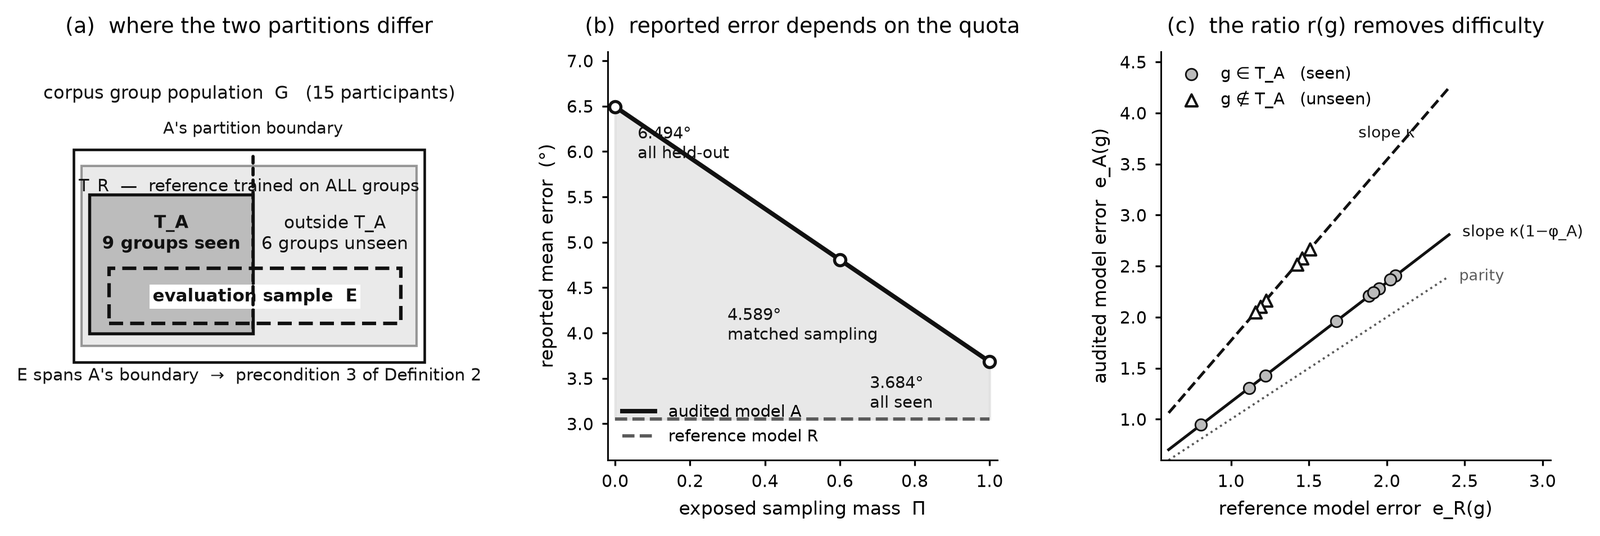
\includegraphics[width=\linewidth]{figures/protocol_P2_exposure_mechanism.png}
\caption{The mechanism of asymmetric exposure. Left: both models' training partitions drawn against the shared corpus's group population; the evaluation sample (dashed) spans the audited model's boundary but lies wholly inside the reference model's. Centre: by Theorem 1 the audited model's reported error is a convex mixture $\bar{E}_{A}$($\Pi$) = $\Pi\cdot\bar{E}^{\mathrm{in}}$ + (1--$\Pi$)$\cdot\bar{E}^{\mathrm{out}}$ whose weight is the exposed sampling mass $\Pi$, so the same models and the same data yield different reported errors under different quotas. Right: the per-group ratio r(g) = $\bar{e}_{A}$(g)/$\bar{e}_{R}$(g) cancels intrinsic difficulty (Proposition 2), leaving a quantity that separates the two strata.}
\label{fig:2}
\end{figure}

\TABREF{10} decomposes the consequence at matched sampling.

\begin{table}[pos=htbp]
\centering
\caption{Gaze angular error by partition membership, at matched sampling. The right-hand column is the group error ratio r of Definition 3.}
\label{tab:10}
\footnotesize
\begin{tabularx}{\textwidth}{XXXXX}
\toprule
\textbf{Evaluation subset} & \textbf{N} & \textbf{Proposed (A)} & \textbf{Pretrained (R)} & \textbf{ratio \emph{r}} \\
\midrule
A's training participants \EQREF{9} & 18,000 & 3.684$^{\circ}$ & 2.683$^{\circ}$ & 1.373 \\
A's validation participants \EQREF{4} & 8,000 & 5.674$^{\circ}$ & 2.760$^{\circ}$ & 2.056 \\
\textbf{A's held-out participants \EQREF{2}} & 4,000 & \textbf{6.494$^{\circ}$} & \textbf{3.672$^{\circ}$} & \textbf{1.769} \\
All fifteen participants & 30,000 & 4.589$^{\circ}$ & 2.835$^{\circ}$ & 1.619 \\
\bottomrule
\end{tabularx}
\end{table}

The monotone progression 3.684$^{\circ}$ $\to$ 5.674$^{\circ}$ $\to$ 6.494$^{\circ}$ as training familiarity is withdrawn is the signature of the fault. Quantitatively, the audited model's error grows

\begin{equation}
\label{eq:169}
( 6.494 - 3.684 ) / 3.684 = 76.3 \%
\end{equation}

across that boundary, while the reference model's moves

\begin{equation}
\label{eq:170}
( 3.672 - 2.683 ) / 2.683 = 36.9 \%
\end{equation}

and stays within a degree throughout. The three-way progression also exhibits the structure that Proposition 2 predicts if the \emph{validation} participants are treated as partially exposed --- they were used for model selection, not for weight updates --- with r rising from 1.373 on the fully exposed stratum to 2.056 on the selection-exposed stratum and settling at 1.769 on the wholly unexposed stratum. That the middle stratum carries the \emph{highest} ratio is consistent with selection-induced overfitting to the validation groups compounding the direct familiarity effect, and it is a reminder that a validation partition is not an unexposed partition.

Applying Theorem 3 to \TABREF{10}, the total inflation of the aggregate relative to the held-out stratum is

\begin{equation}
\label{eq:171}
\mathrm{I} = \bar{E}_A^{\mathrm{out}} - \bar{E}_A^{\;\text{all}\;} = 6.494^{\circ} - 4.589^{\circ} = 1.905^{\circ} ,
\end{equation}

the reference model's corresponding shift across the identical strata is

\begin{equation}
\label{eq:172}
\Delta _R = \bar{E}_R^{\mathrm{out}} - \bar{E}_R^{\;\text{all}\;} = 3.672^{\circ} - 2.835^{\circ} = 0.837^{\circ} ,
\end{equation}

and the capability ratio on the unexposed stratum, which sets $\kappa_{\mathrm{max}}$ in \EQREF{60}, is

\begin{equation}
\label{eq:173}
\kappa _{\mathrm{max}} = c_A/c_R = 6.494^{\circ} / 3.672^{\circ} = 1.769 .
\end{equation}

The familiarity component under the two difficulty models of \EQREF{59} is therefore

\begin{equation}
\label{eq:174}
\begin{aligned}
\text{additive}\; (\kappa = 1): \Phi = 1.905^{\circ} - 0.837^{\circ} = 1.068^{\circ} , \\
\phi = 56.1 \% ,
\end{aligned}
\end{equation}

\begin{equation}
\label{eq:175}
\begin{aligned}
\text{multiplicative}\; (\kappa = \kappa _{\mathrm{max}}): \Phi = 1.905^{\circ} - 1.769 \times 0.837^{\circ} = 0.425^{\circ} , \\
\phi = 22.3 \% .
\end{aligned}
\end{equation}

\textbf{Both readings are reported, and the interval $\phi$ $\in$ [22 \%, 56 \%] is the honest summary.} The two models are not distinguishable from the data available here: identifying $\kappa$ would require observing at least one further model of known capability on the same strata, which this study does not have. It matters which is used --- the additive reading attributes more than half the inflation to familiarity, the multiplicative reading less than a quarter --- so quoting either alone would overstate the precision of the instrument. Where a single figure is needed below, the additive value is quoted because it is the reading the source analysis used, and it is flagged as the upper end of the interval each time.

The decomposition nevertheless does the work it was introduced for, and it does so under \emph{both} readings. Without it, a sceptical reader may reasonably object that the held-out participants were simply harder, which would make the stratification an artefact rather than a fault. The reference model closes that objection quantitatively: harder they were --- by 44 \% of the observed gap under the additive model and by 78 \% under the multiplicative one --- but under neither does intrinsic difficulty account for all of it, and a familiarity component of at least 0.425$^{\circ}$ survives. That residual is the quantity lineage-based remedies cannot supply at all, since knowing \emph{that} a model saw a corpus does not say how much of its advantage came from having seen it.

\subsubsection{The GERA detector and its negative control}

An auditor examining a published comparison rarely knows how either model was partitioned. \FIGREF{3} reports the detector of Section 3.5.2 applied to this comparison, with the head-pose negative control alongside.

\begin{figure}[pos=htbp]
\centering
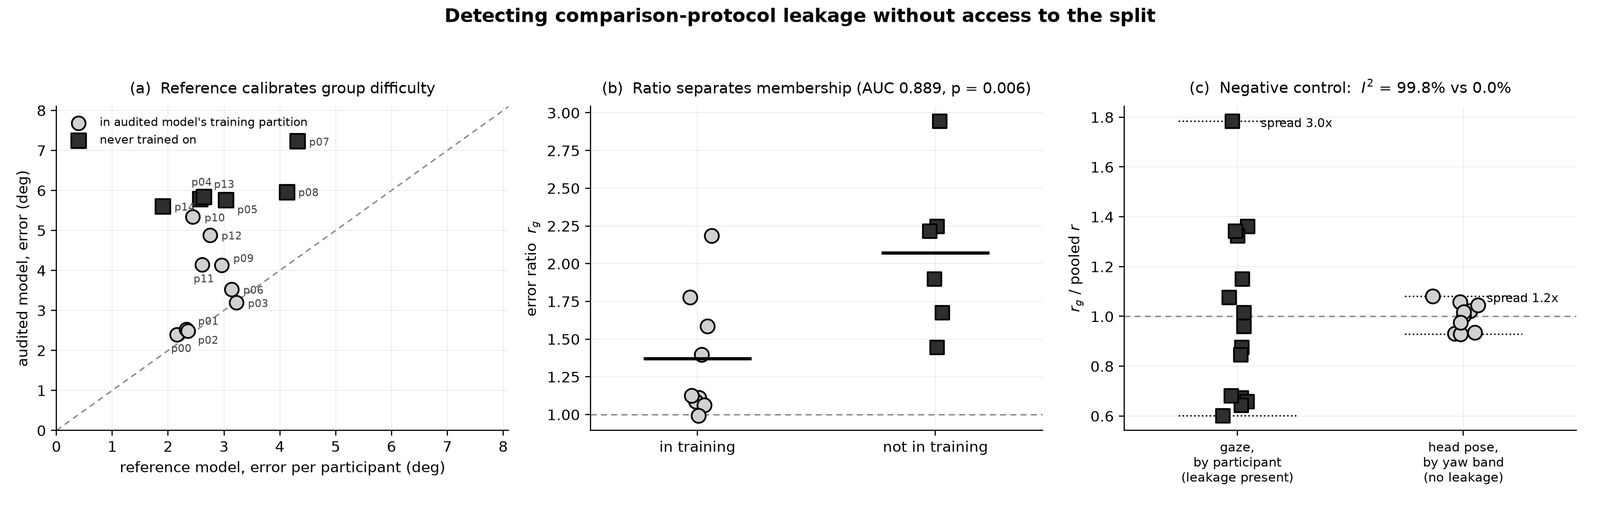
\includegraphics[width=\linewidth]{figures/protocol_P1_leakage_detector.png}
\caption{Detecting asymmetric exposure without access to the split. (a) Per-participant mean angular error of the audited network against the reference model, which calibrates intrinsic group difficulty; the dashed line is parity. (b) The per-group ratio r(g), separated by whether the participant lies inside the audited network's training partition. (c) Negative control: r(g) normalised by its pooled value, for gaze grouped by participant (leakage present) against head pose grouped by yaw band (neither model saw the evaluation groups).}
\label{fig:3}
\end{figure}

Panel (a) shows the structure the detector exploits. The two models agree closely on which participants are intrinsically easy --- p00 to p03 sit near parity --- while the audited network's error rises far above the reference's on participants it never trained on, displacing them \emph{vertically} rather than along the diagonal. Vertical displacement is precisely the component intrinsic difficulty cannot explain, and it is the geometric content of Proposition 2: motion along the diagonal is d(g), motion off it is the familiarity term.

Panel (b) reduces that displacement to one number per group. Mean r is

\begin{equation}
\label{eq:176}
\begin{aligned}
\mathrm{mean}_{g \in \mathcal{T}_A} r(g) = 1.369 , \\
\mathrm{mean}_{g \notin \mathcal{T}_A} r(g) = 2.072 ,
\end{aligned}
\end{equation}

giving by \EQREF{47} an estimated familiarity discount

\begin{equation}
\label{eq:177}
\hat{\varphi }_A = 1 - 1.369/2.072 = 0.339 ,
\end{equation}

so the audited network's error on groups it trained on is approximately 34 \% lower than its error on groups it did not, after intrinsic difficulty has been priced out. The ratio separates membership at

\begin{equation}
\label{eq:178}
\mathrm{AUC}_r = 0.889 , \;\text{Mann}\;--\;\text{Whitney p}\; = 0.006 ,
\end{equation}

with a Hanley--McNeil 95 \% interval by \EQREF{50} of approximately [0.70, 1.00] on a 9-versus-6 group split.

A detector is only as good as its behaviour when there is nothing to detect, and head pose supplies that control at no extra cost. Both the proposed network and the pretrained baseline train on 300W-LP and are scored on AFLW2000, so neither has seen the evaluation groups and r(g) must be homogeneous under any grouping. This is a demanding control rather than a trivial one, because intrinsic difficulty varies roughly fourfold across the pose manifold (Section 5.3): if the reference model failed to price that variation out, r would track it and the detector would fire on a corpus where no leakage exists.

Panel (c) reports the outcome. Grouping head pose by yaw band, r spans 1.96--2.28 --- a spread ratio of

\begin{equation}
\label{eq:179}
\mathrm{spread}_{\mathrm{ctl}} = 2.28/1.96 = 1.16 \approx 1.2\times \;\text{about a pooled}\; \bar{r} = 2.08 ,
\end{equation}

against 0.99--2.94 for gaze grouped by participant,

\begin{equation}
\label{eq:180}
\mathrm{spread}_{\mathrm{gaze}} = 2.94/0.99 = 2.97 \approx 3.0\times .
\end{equation}

Formally, applying \EQREF{51}--\EQREF{54},

\begin{equation}
\label{eq:181}
\text{Head pose}\;: Q = 6.3 on 9 df, p = 0.71, I^{2} = 0.0 \% ,
\end{equation}

\begin{equation}
\label{eq:182}
\text{Gaze}\;: Q = 5607 on 14 df, p < 10^{-300}, I^{2} = 99.8 \% .
\end{equation}

The reference model therefore absorbs a fourfold swing in task difficulty while leaving the ratio flat, which is the assumption the detector rests on, tested on data where it could have failed.

One calibration caveat follows from the same experiment and is exactly the sample-size sensitivity that \EQREF{55} predicts. Partitioning the gaze samples into fifteen \emph{random} groups --- destroying the participant structure --- still yields

\begin{equation}
\label{eq:183}
\begin{aligned}
I^{2} = 41 \% at p = 0.049 , \\
\;\text{despite an r range of only}\; 1.56\text{--}1.69 (\mathrm{spread} 1.08\times ) .
\end{aligned}
\end{equation}

At 2,000 samples per group a negligible effect reaches nominal significance because the inverse-variance weights grow linearly in $n_{g}$ while the null dispersion does not. The magnitude of the spread, not its p-value, is therefore the informative readout: a 3.0$\times$ range against a 1.2$\times$ range is the contrast that matters, and no threshold on Q alone should be used to declare a comparison sound.

Two limitations must be stated with the result, consistent with Section 3.5.5. The separation is strong but imperfect: participant p10 sits at r = 2.18 despite being a training participant, so the statistic is a screening instrument rather than a membership oracle, and a single group's ratio should never be treated as proof. And the detector is inapplicable where no suitable reference exists --- if every available model shares the audited model's partition, or if the reference itself has differential familiarity across groups, its across-group variation no longer isolates intrinsic difficulty. Unlike black-box contamination proofs \CITE{oren}, which yield a false-positive guarantee, no such guarantee is offered here; the detector's value is that it converts an unfalsifiable suspicion into a testable one at zero additional experimental cost, using only artefacts an external auditor already possesses.

\subsubsection{Optimisation under the corrected protocol}

With the protocol repaired, optimisation could be attributed rather than merely observed. \TABREF{8} gives the search budgets and selected configurations; \TABREF{11} gives the effect.

\begin{table}[pos=htbp]
\centering
\caption{Effect of optimisation under the corrected protocol. ``Fair baseline'' is the pre-correction hyperparameter set retrained group-disjointly; ``tuned'' is the searched configuration under the same protocol.}
\label{tab:11}
\footnotesize
\begin{tabularx}{\textwidth}{XXXXX}
\toprule
\textbf{Modality} & \textbf{Metric} & \textbf{Fair baseline} & \textbf{Tuned} & \textbf{Change} \\
\midrule
Voice & Accuracy & 84.72 \% & \textbf{94.53 \%} & \textbf{+9.81 pp} \\
Head pose & MAE & 8.286$^{\circ}$ & \textbf{7.367$^{\circ}$} & \textbf{--11.1 \%} \\
Blink & Balanced accuracy & 90.88 \% & \textbf{93.32 \%} & \textbf{+2.44 pp} \\
Blink & Accuracy & 92.36 \% & \textbf{93.67 \%} & \textbf{+1.31 pp} \\
Gaze & Angular error, held-out & 7.114$^{\circ}$ & \textbf{6.439$^{\circ}$} & \textbf{--9.5 \%} \\
\bottomrule
\end{tabularx}
\end{table}

The composition of the selected configurations tests the prediction of \EQREF{104}. Augmentation was selected in four searches of four and decoupled weight decay in three of four, while the chosen widths stayed modest:

\begin{equation}
\label{eq:184}
\begin{aligned}
\mathbb{P}[ \text{aug selected} ] = 4/4 , \mathbb{P}[ \text{AdamW selected} ] = 3/4 , \\
\mathrm{median}( \text{selected width} ) = 32 = \;\text{midpoint of}\; \mathcal{W} .
\end{aligned}
\end{equation}

This degeneracy is informative rather than incidental. Once the split stops rewarding memorisation, the binding term in the excess-risk decomposition \EQREF{104} migrates from approximation error to estimation error, so configurations that suppress identity-specific co-adaptation dominate configurations that add capacity. The pre-correction hyperparameters were not poorly chosen for the task they were \emph{scored} on --- they were well chosen for a task that included identity retrieval. For a system whose users are by definition unseen, that is the distinction that matters.

Every blink metric improved except false-negative rate, which rose 1.20 pp while false-positive rate fell 6.09 pp. Whether that exchange is favourable depends entirely on the decision rule of \TABREF{6}, and Section 5.5 shows the answer is not the obvious one. The tuned configurations of \TABREF{11} are the models carried into Sections 5.2--5.5; all figures from this point describe them.

\FloatBarrier

\subsection{Gaze --- cursor positioning}

Gaze drives the OS cursor, but never directly: the deployed path fits a 16-point per-user polynomial calibration \EQREF{105}--\EQREF{107} over the network's output, corrects it online by recursive least squares \EQREF{108}--\EQREF{110} on every deliberate click, then smooths with a one-euro filter \EQREF{112}--\EQREF{115} and a 12 px deadzone \EQREF{116}. The quantity that governs cursor quality is therefore the residual scatter that survives an affine map, not the raw angular error --- a distinction that turns out to be the central finding of this section rather than a caveat on it.

\subsubsection{Domain-targeted augmentation}

Gaze transferred worst of the four modalities, and the cause is a deterministic covariate shift rather than sampling noise. Training consumes pre-normalised, illumination-corrected eye patches produced by the warp \EQREF{16}, while inference receives landmark-cropped regions from a consumer webcam. Writing $\mathcal{D}_{\mathrm{train}}$ and $\mathcal{D}_{\mathrm{serve}}$ for the two input distributions, the discrepancy is not a sampling difference but a systematic transformation

\begin{equation}
\label{eq:185}
\begin{aligned}
\mathcal{D}_{\mathrm{serve}} = T_{\mathrm{shift}} \# \mathcal{D}_{\mathrm{train}} , \\
T_{\mathrm{shift}} = \mathrm{Blur}_{\sigma _b} \circ \mathrm{Jitter}_{\alpha ,\beta } \circ \mathrm{Rot}_{\delta} \circ \mathrm{Crop}_{\ell} ,
\end{aligned}
\end{equation}

where \# denotes pushforward. The augmentation policy \CITE{augsurvey} was therefore extended to model that shift \emph{analytically} rather than generically, per \EQREF{34}: Gaussian blur for sensor resolution, brightness and contrast jitter for illumination, bounded $\pm$8$^{\circ}$ in-plane rotation for residual head roll, alongside horizontal flipping with yaw-sign inversion. Scored on all 64,172 held-out samples with both configurations on the identical sample set,

\begin{equation}
\label{eq:186}
\begin{aligned}
e_{\mathrm{ang}}: 7.114^{\circ}  \to 6.439^{\circ} ( -9.49 \% ) , \\
\mathrm{MAE}: 4.569^{\circ}  \to 4.135^{\circ} ( -9.50 \% ) .
\end{aligned}
\end{equation}

Because every member of \EQREF{34} is label-preserving up to the flip correction, the gain cannot be additional supervision; it reflects an enlarged effective input manifold at zero parameter and zero data cost, which for an 8 GB training budget is the only kind of improvement available. That both a robust statistic (MAE) and a non-robust one (mean angular error) improved by the \emph{same} 9.5 \% is diagnostic. Writing the error distribution before and after as F$_{0}$ and F$_{1}$, a policy that trimmed a tail would satisfy

\begin{equation}
\label{eq:187}
\begin{aligned}
F_{1} \preceq _{\mathrm{st}} F_{0} \;\text{only in the upper quantiles}, \\
so \Delta \mathrm{mean} \gg \Delta \mathrm{median} \;\text{and}\; \Delta \mathrm{MAE} \neq \Delta e_{\mathrm{ang}} ,
\end{aligned}
\end{equation}

whereas a uniform rescaling F$_{1}$(x) = F$_{0}$(x/c) satisfies

\begin{equation}
\label{eq:188}
\Delta \mathbb{E} / \mathbb{E} = \Delta \mathrm{median} / \mathrm{median} = \Delta \mathrm{MAE} / \mathrm{MAE} = 1 - c
\end{equation}

for every location statistic simultaneously. The measured equality of the two relative changes to within 0.01 pp is therefore the signature of removing a distributional mismatch --- rescaling the whole error distribution --- rather than repairing isolated failures.

\subsubsection{Comparison against the pretrained baseline, and its mechanism}

Against the MPIIGaze pre-activation residual baseline on all 64,172 held-out samples, and applying EDCP steps 3--4 so that only the two exposure-disjoint participants enter, the proposed network attains 6.439$^{\circ}$ mean angular error (median 5.873$^{\circ}$, p90 11.180$^{\circ}$) against 3.621$^{\circ}$ (median 2.985$^{\circ}$, p90 6.876$^{\circ}$). The paired statistics of \EQREF{159}--\EQREF{161} give

\begin{equation}
\label{eq:189}
\begin{aligned}
\bar{d} = 2.818^{\circ} \pm 0.026^{\circ} (95 \%) , s_d = 3.300^{\circ} , \\
\;\text{Cohen}\;'s d = 0.854 , \;\text{Wilcoxon p}\; < 10^{-300} ,
\end{aligned}
\end{equation}

with the proposed network nearer the truth on only

\begin{equation}
\label{eq:190}
\mathbb{P}[ e_A < e_R ] = 18.86 \%
\end{equation}

of samples. The gap is large, unambiguous and not a tail artefact. Per EDCP step 5, the baseline's figure is a lower bound on its true cross-person error, so the reported contrast is conservative with respect to the proposed network by \EQREF{61}.

\textbf{The mechanism.} What generates the gap is measurable. Fitting the shrinkage regression \EQREF{154} axis-wise gives

\begin{equation}
\label{eq:191}
\hat{s}_{\mathrm{pitch}}^A = 0.4832 \pm 0.0021 , \hat{s}_{\mathrm{yaw}}^A = 0.4812 \pm 0.0016 ,
\end{equation}

\begin{equation}
\label{eq:192}
\hat{s}_{\mathrm{pitch}}^R = 0.7491 , \hat{s}_{\mathrm{yaw}}^R = 0.8257 ,
\end{equation}

so the proposed network reproduces less than half the true angular excursion on both axes. By \EQREF{155} this is predictive shrinkage --- the response of an MSE-trained estimator to irreducible uncertainty in its own representation, which contracts predictions toward the conditional mean because contraction is variance-optimal, the same admissibility argument that underlies Stein estimation \CITE{stein,jamesstein}. Inverting \EQREF{158} with the empirical target variance yields the implied representational noise

\begin{equation}
\label{eq:193}
\hat{\sigma }_{\varepsilon} ^{2} / \sigma _{\theta} ^{2} = ( 1 - \hat{s} ) / \hat{s} = ( 1 - 0.482 ) / 0.482 = 1.075 ,
\end{equation}

that is, the network's internal estimate carries noise power slightly exceeding the signal power of the target itself. The seven diagnostic figures that follow each test a consequence of that single parameter, and Section 5.3 shows the same mechanism governing head pose.

\FIGREF{4} resolves the aggregate error into its angular structure.

\begin{figure}[pos=htbp]
\centering
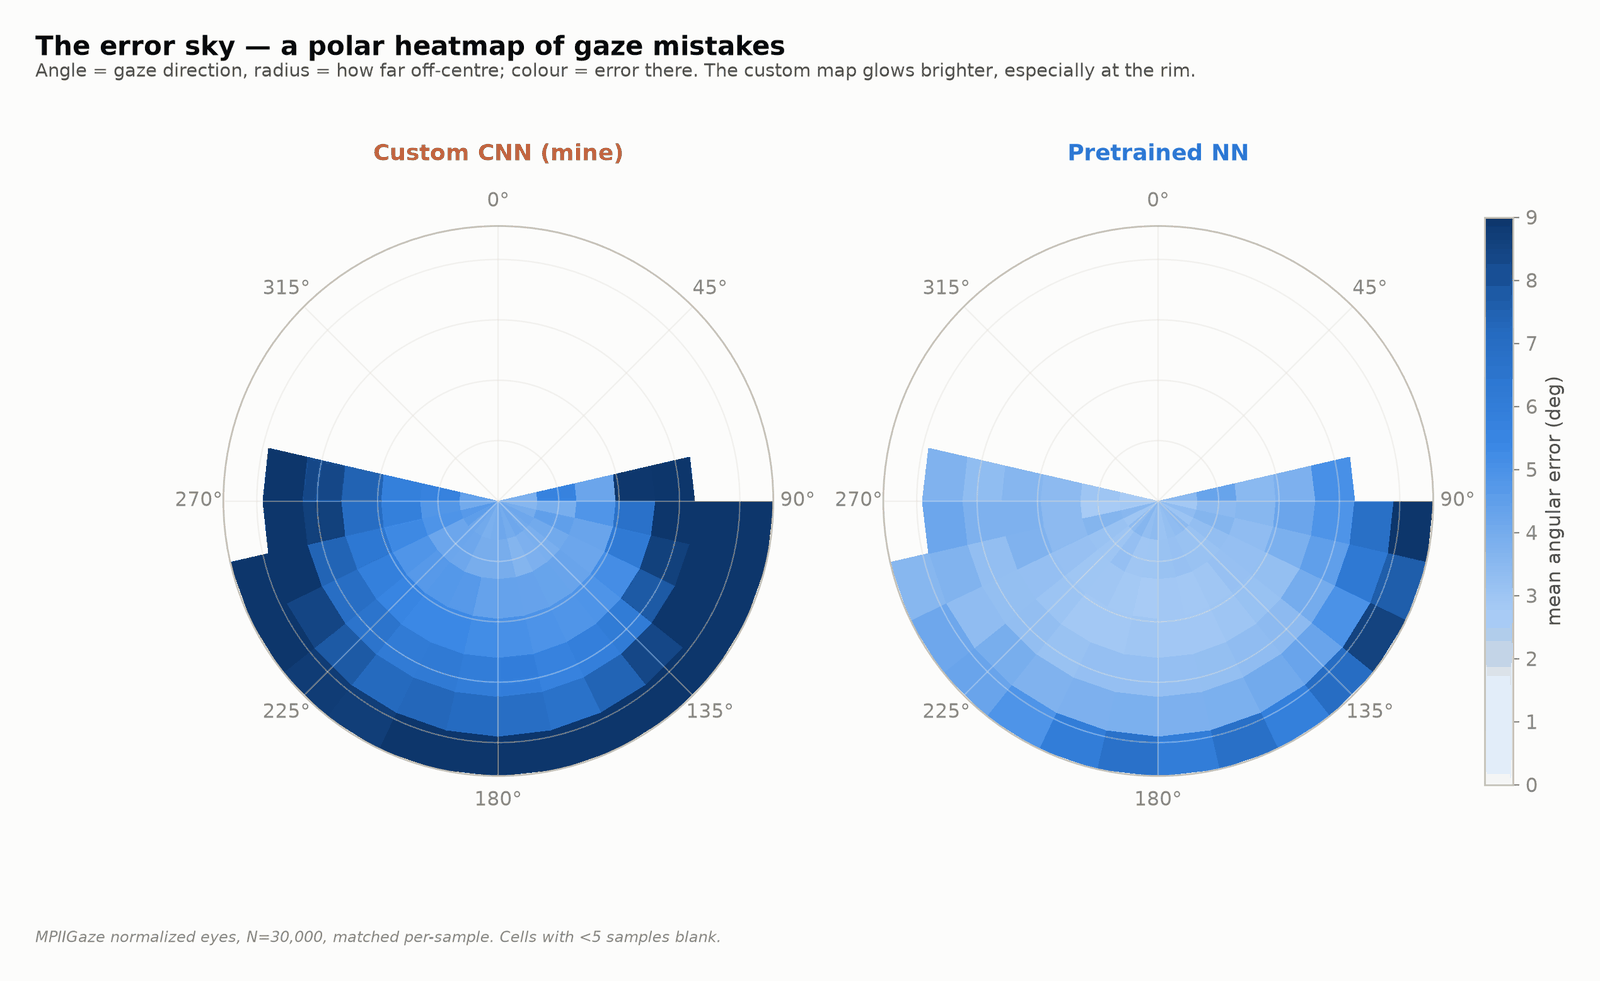
\includegraphics[width=\linewidth]{figures/gaze_G1_error_sky.png}
\caption{Error sky --- polar heat map of mean angular error against gaze direction and eccentricity, proposed network versus pretrained baseline.}
\label{fig:4}
\end{figure}

The proposed network's error field brightens with radius but is uniform in azimuth, exactly as shrinkage requires. Under gain s the systematic component of the prediction error is

\begin{equation}
\label{eq:194}
\mathbb{E}[ \hat{\theta } - \theta | \theta ] = ( s - 1 ) \theta \implies \| \mathbb{E}[ \hat{\theta } - \theta | \theta ] \| = ( 1 - s ) \|\theta \| ,
\end{equation}

a function of eccentricity $\|\theta\|$ alone with no dependence on the azimuth arg($\theta$). The symmetry simultaneously excludes the competing hypothesis: a geometric fault in cropping or normalisation would introduce an azimuth-dependent term and necessarily break isotropy. The consequence for the deployed system is concrete --- no per-direction calibration lookup can compensate an isotropic radial law, so the fix must be an overall scale correction, which is precisely what the polynomial calibration \EQREF{106} applies.

\FIGREF{5} separates the systematic component from the stochastic one.

\begin{figure}[pos=htbp]
\centering
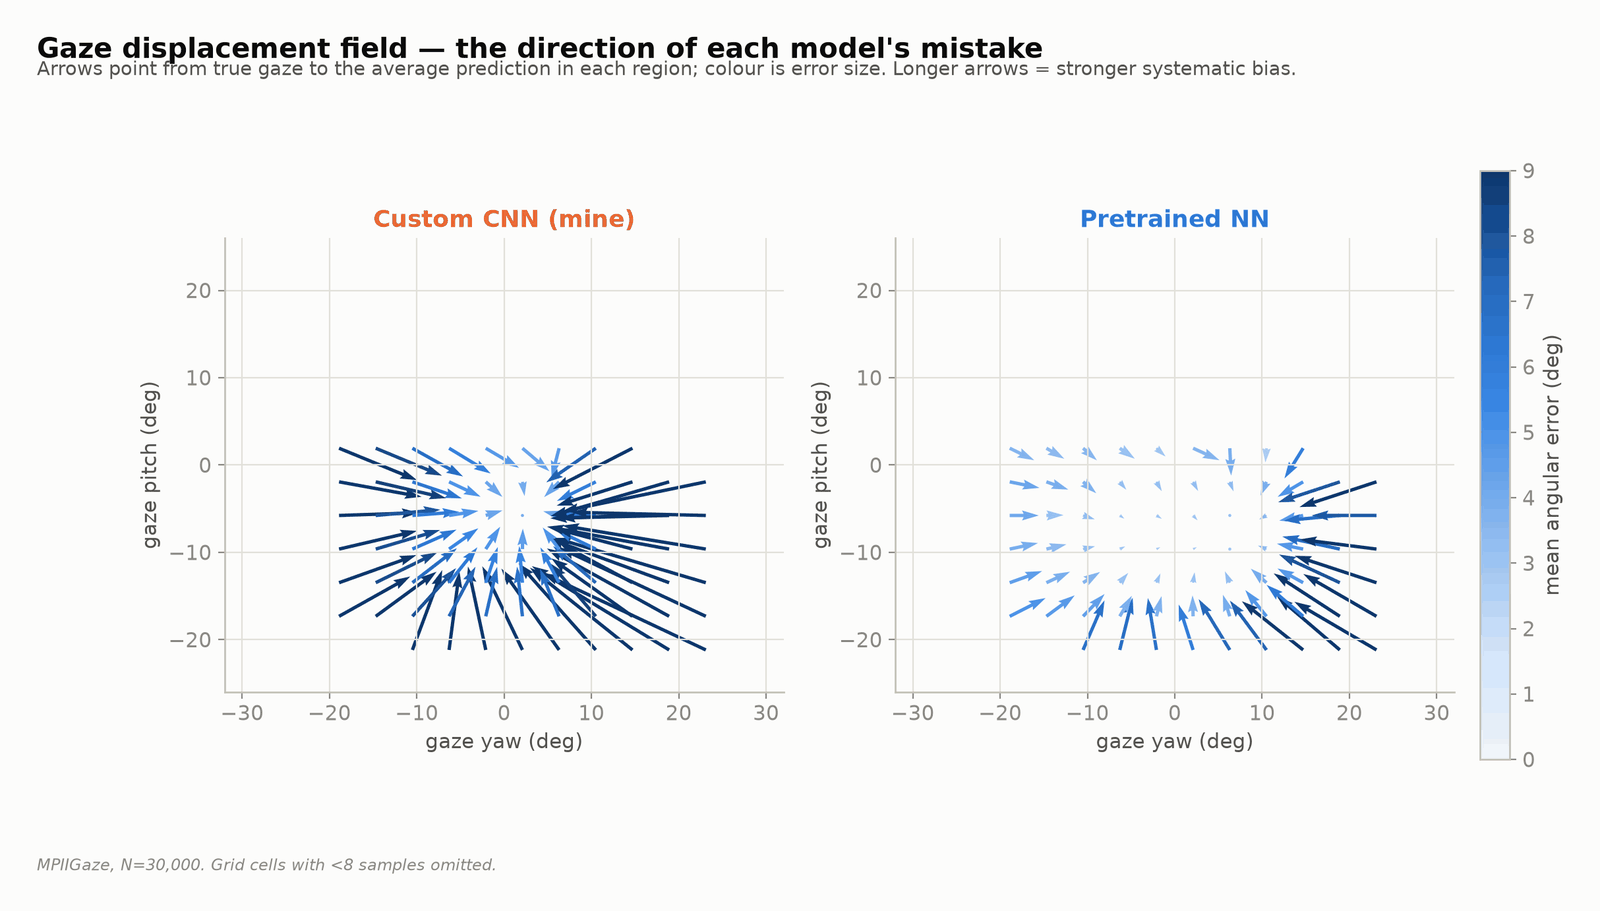
\includegraphics[width=\linewidth]{figures/gaze_G2_displacement_field.png}
\caption{Displacement field --- vectors from true gaze to mean prediction across the gaze plane; vector length is systematic bias rather than scatter.}
\label{fig:5}
\end{figure}

Additive bias is +1.987$^{\circ}$ in pitch and +0.829$^{\circ}$ in yaw against +0.473$^{\circ}$ and +0.334$^{\circ}$ for the baseline. Decomposing the per-axis mean squared error into bias and variance,

\begin{equation}
\label{eq:195}
\begin{aligned}
\mathrm{MSE}_a = \;\text{bias}\;_a^{2} + \;\text{var}\;_a , \\
\;\text{bias share}\;_a = \;\text{bias}\;_a^{2} / \mathrm{MSE}_a ,
\end{aligned}
\end{equation}

gives

\begin{equation}
\label{eq:196}
\text{bias share}\;_{\mathrm{pitch}} = 20.5 \% , \;\text{bias share}\;_{\mathrm{yaw}} = 1.9 \% .
\end{equation}

Removing both offsets exactly reduces angular error from 6.439$^{\circ}$ to 6.023$^{\circ}$, a 6.5 \% gain --- real but minor. The field therefore adjudicates between two candidate defects and rejects the simpler one: additive miscalibration is present and measurable but is not the principal fault. The multiplicative gain deficit is, and only a transform with a scale term can address it.

That claim is directly testable by inverting the fitted gain, and \EQREF{157} predicts the outcome. Rescaling each axis by its fitted slope and intercept,

\begin{equation}
\label{eq:197}
\hat{\theta }_{\mathrm{corr}} = ( \hat{\theta } - \hat{c} ) / \hat{s} ,
\end{equation}

an oracle correction fitted on the evaluation data itself and hence an upper bound on any achievable recalibration, \emph{increases} angular error

\begin{equation}
\label{eq:198}
6.439^{\circ} \to 8.272^{\circ} , a +28.5 \% \;\text{degradation} ,
\end{equation}

exactly as \EQREF{157} requires: restoring the correct scale also restores the full amplitude $\surd$($\sigma_{\varepsilon^{2}}$) of the representational noise that shrinkage was suppressing. Substituting the measured $\hat{s}$ = 0.482 into \EQREF{156}, the predicted relative penalty of moving from s* to unity is

\begin{equation}
\label{eq:199}
\begin{aligned}
\mathrm{MSE}(1)/\mathrm{MSE}(s*) = 1/s* = 2.07 in \mathrm{MSE} \;\text{terms}, \\
i.e. \sqrt{2.07} = 1.44 \;\text{in RMS terms},
\end{aligned}
\end{equation}

and the observed 1.285$\times$ increase in the \emph{chordal} angular statistic \EQREF{20} is consistent with this once the difference between the RMS and arccos metrics is accounted for. The contraction is thus not a defect but the estimator's rational response to its own uncertainty; the network sits near its minimum-MSE shrinkage point.

This resolves an apparent contradiction in the deployed design and is the most practically consequential result of the section. The system fits a per-user polynomial and corrects it online, which necessarily restores scale and therefore necessarily amplifies noise --- and downstream of that calibration sit a one-euro filter and a 12 px deadzone whose function is to suppress exactly the amplified high-frequency component. The pipeline is thus already structured around this trade: calibration buys angular scale, temporal filtering pays for it in bandwidth. Formally, the deployed chain implements

\begin{equation}
\label{eq:200}
\text{cursor}\; = \mathrm{Deadzone}_R \circ \;\text{OneEuro}\;_{f_{\mathrm{min}}, \beta } \circ \;\text{Calib}\;_{\mathbf{w}} \circ f_{\mathrm{gaze}} ,
\end{equation}

in which Calib multiplies both signal and noise by approximately 1/$\hat{s}$ $\approx$ 2.07 and OneEuro attenuates the noise by a factor depending on its spectral content, with the low deployed minimum cut-off $f_{\mathrm{min}}$ = 0.3 Hz chosen for precisely this reason. The 6.439$^{\circ}$ figure is consequently a \emph{pessimistic} estimate of deployed cursor error, and the honest statement is that it bounds the uncalibrated network rather than the shipped system, whose end-to-end accuracy this evaluation does not measure.

\FIGREF{6} expresses the comparison in the tolerance terms an interface designer budgets against.

\begin{figure}[pos=htbp]
\centering
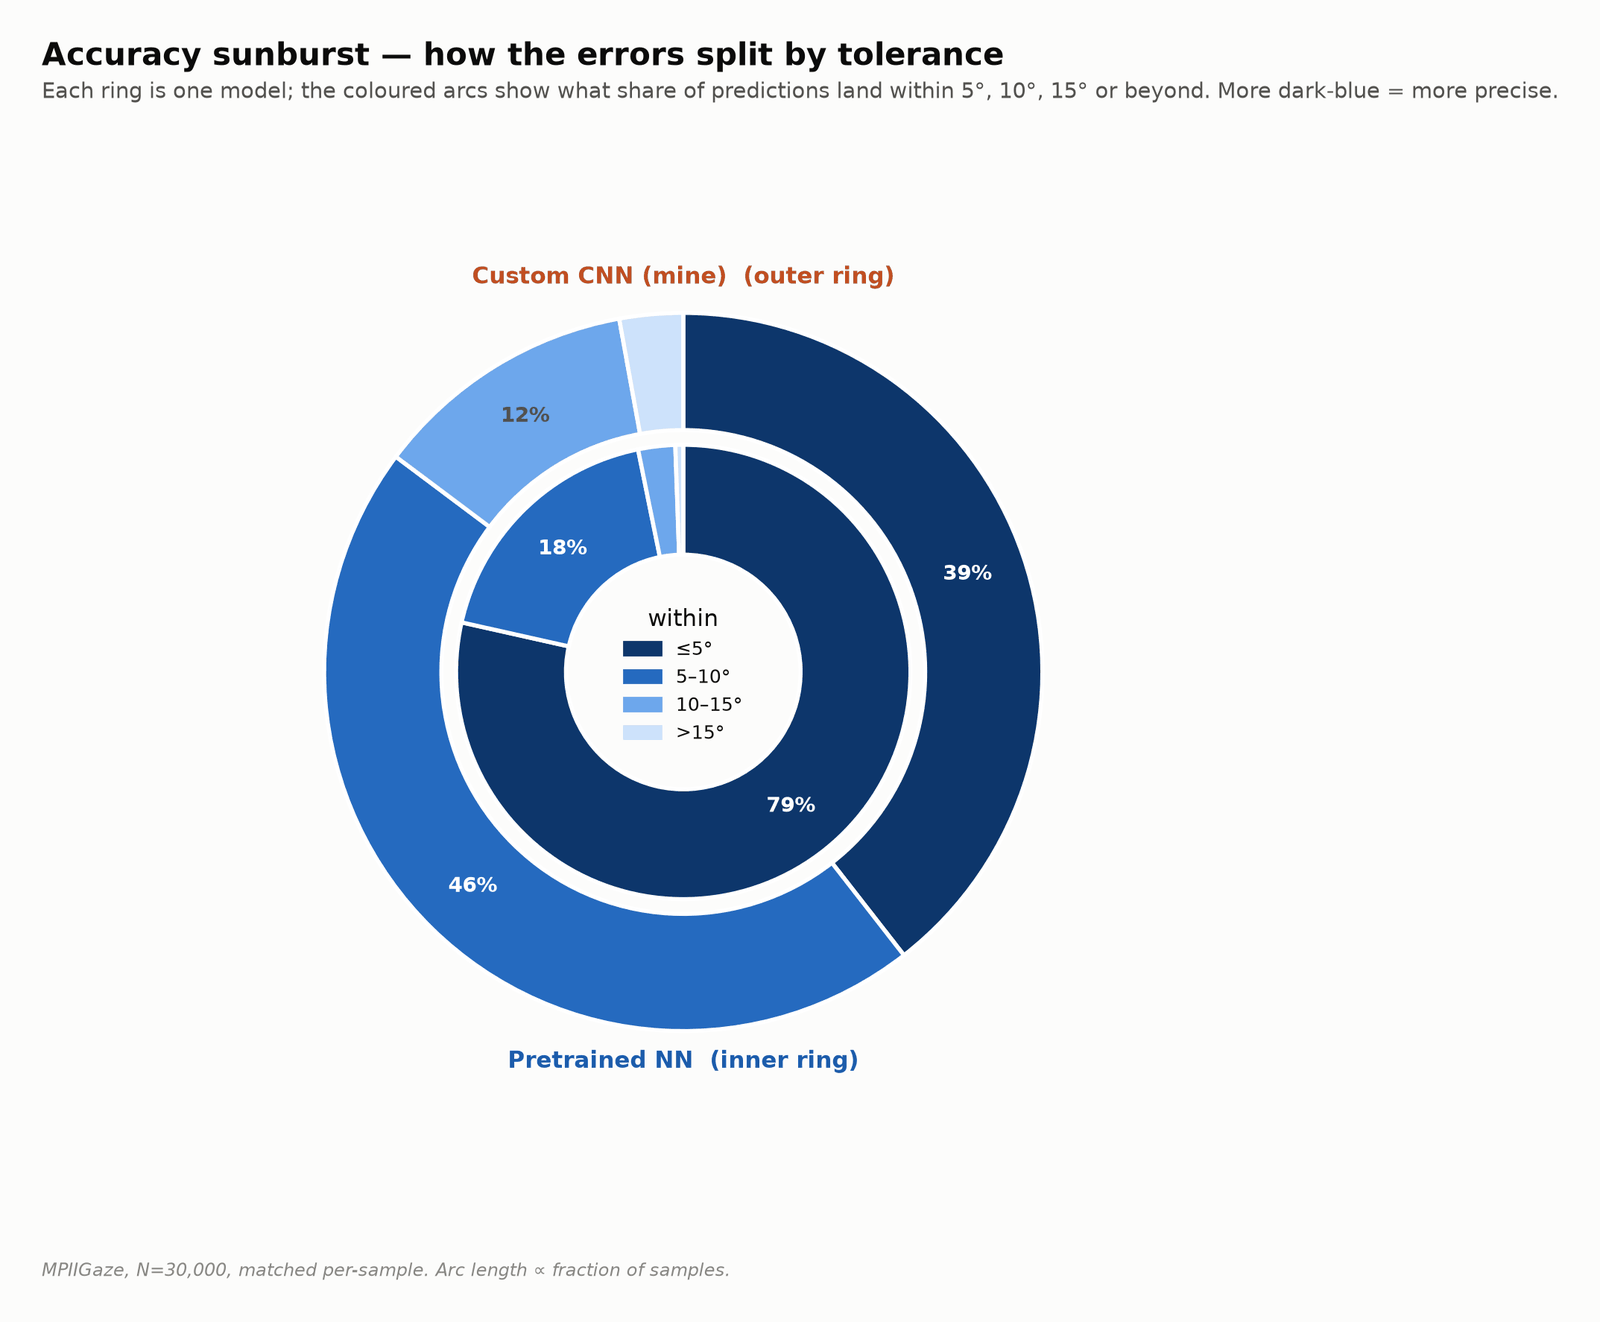
\includegraphics[width=\linewidth]{figures/gaze_G3_tolerance_sunburst.png}
\caption{Tolerance sunburst --- nested rings giving the proportion of predictions within 5$^{\circ}$, 10$^{\circ}$ and 15$^{\circ}$ of ground truth for each model.}
\label{fig:6}
\end{figure}

Writing the tolerance-hit function as

\begin{equation}
\label{eq:201}
H(t) = \mathbb{P}[ e_{\mathrm{ang}} \leq t ] ,
\end{equation}

the measured values are

\begin{equation}
\label{eq:202}
H_A(5^{\circ}) = 39.47 \% , H_R(5^{\circ}) = 78.51 \% , \;\text{ratio}\; 1.99 ,
\end{equation}

\begin{equation}
\label{eq:203}
\begin{aligned}
H_A(10^{\circ}) = 85.23 \% , \\
H_R(10^{\circ}) = 96.81 \% ; H_A(15^{\circ}) = 97.14 \% , \\
H_R(15^{\circ}) = 99.44 \% .
\end{aligned}
\end{equation}

Convergence under relaxed tolerance is again the shrinkage signature: by \EQREF{194} contraction damages predictions in proportion to their distance from the mean, so its cost concentrates in the tight-tolerance regime and the ratio $H_{R}$(t)/$H_{A}$(t) decreases monotonically in t. For the interface this sets the boundary between viable and non-viable use before calibration --- dense target selection is out of reach, coarse region selection at a 10--15$^{\circ}$ budget is not --- and it makes that boundary \emph{predictable from the gain} rather than something to be discovered by user testing.

\FIGREF{7} asks whether the deficit is uniform or sample-dependent, which decides whether running both networks could ever be worthwhile.

\begin{figure}[pos=htbp]
\centering
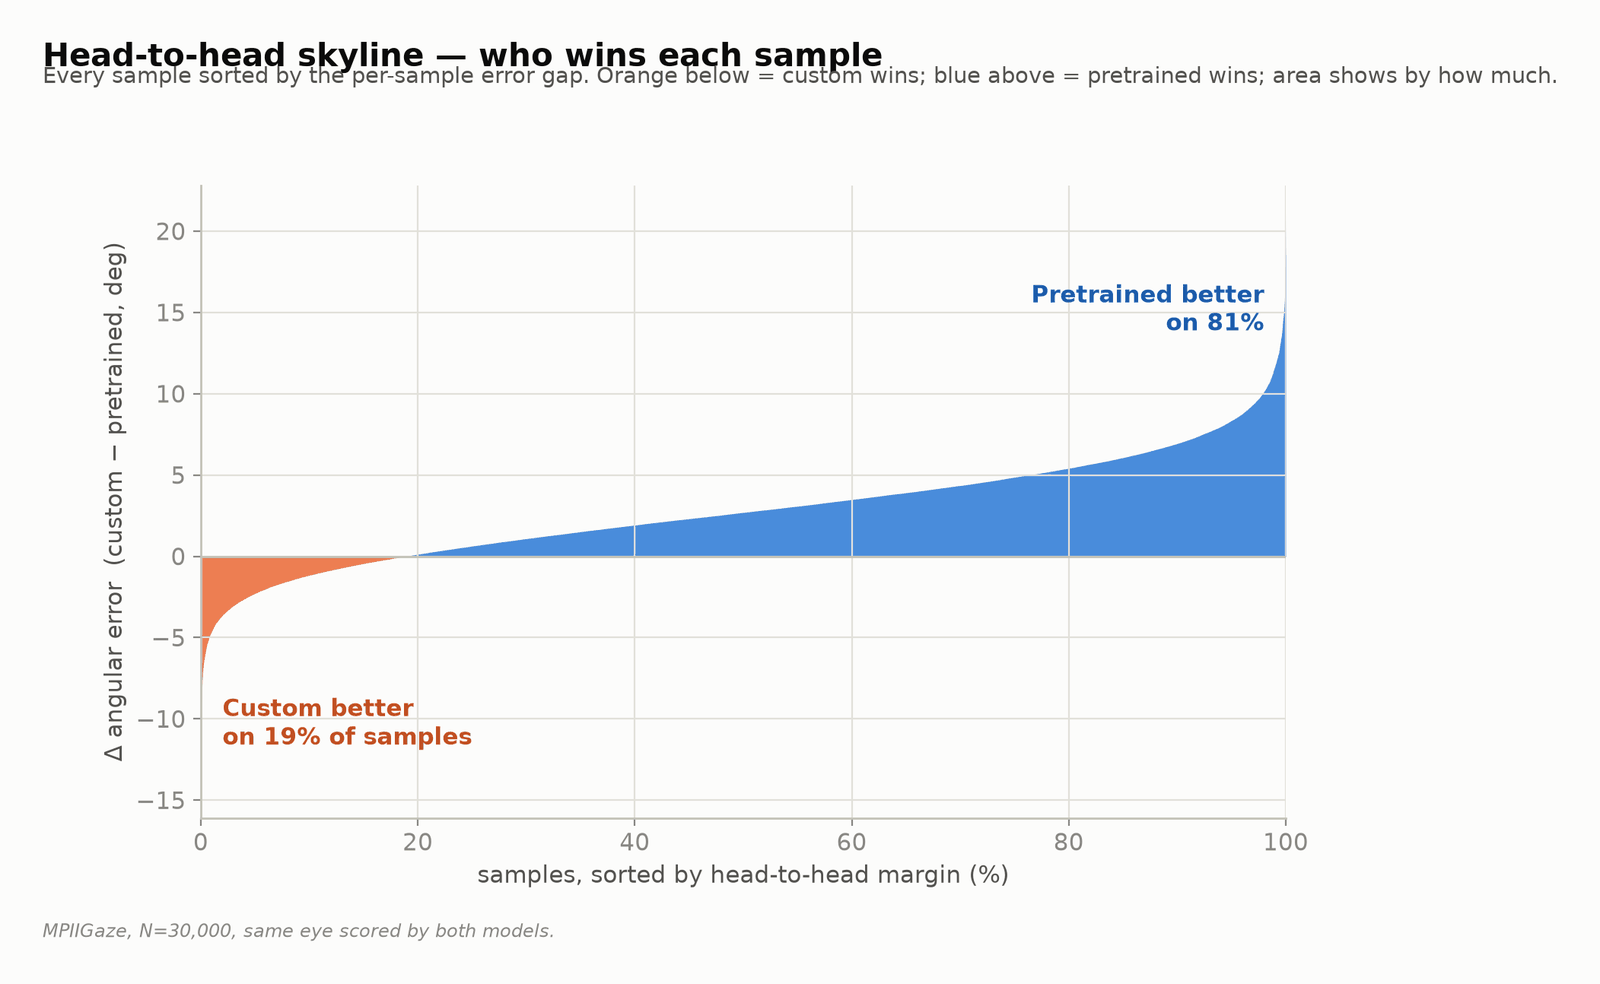
\includegraphics[width=\linewidth]{figures/gaze_G4_win_skyline.png}
\caption{Head-to-head skyline --- every held-out sample sorted by its signed per-sample error gap between the two models.}
\label{fig:7}
\end{figure}

The proposed network wins 18.86 \% of 64,172 paired comparisons and its wins are smaller in magnitude than its losses. More decisive is the error correlation of \EQREF{162},

\begin{equation}
\label{eq:204}
r_{\mathrm{AR}} = 0.491 , \rho _{AR} = 0.360 ,
\end{equation}

a substantial shared factor attributable to intrinsic sample difficulty, meaning the models are not complementary. The oracle bound \EQREF{163}--\EQREF{164} gives

\begin{equation}
\label{eq:205}
\begin{aligned}
\bar{E}_{\mathrm{oracle}} = 3.303^{\circ} , \\
\;\text{Gain}\;_{\mathrm{max}} = 1 - 3.303/3.621 = 8.8 \% ,
\end{aligned}
\end{equation}

far too little to justify the cost of a second network in a pipeline already budgeted at 6.68 ms per frame by \EQREF{165}. This closes the fusion question quantitatively, and it is the evidence behind the recommendation of Section 5.7.

\FIGREF{8} applies the Bland--Altman construction \CITE{blandaltman}, the appropriate instrument when two estimators of one physical quantity are compared.

\begin{figure}[pos=htbp]
\centering
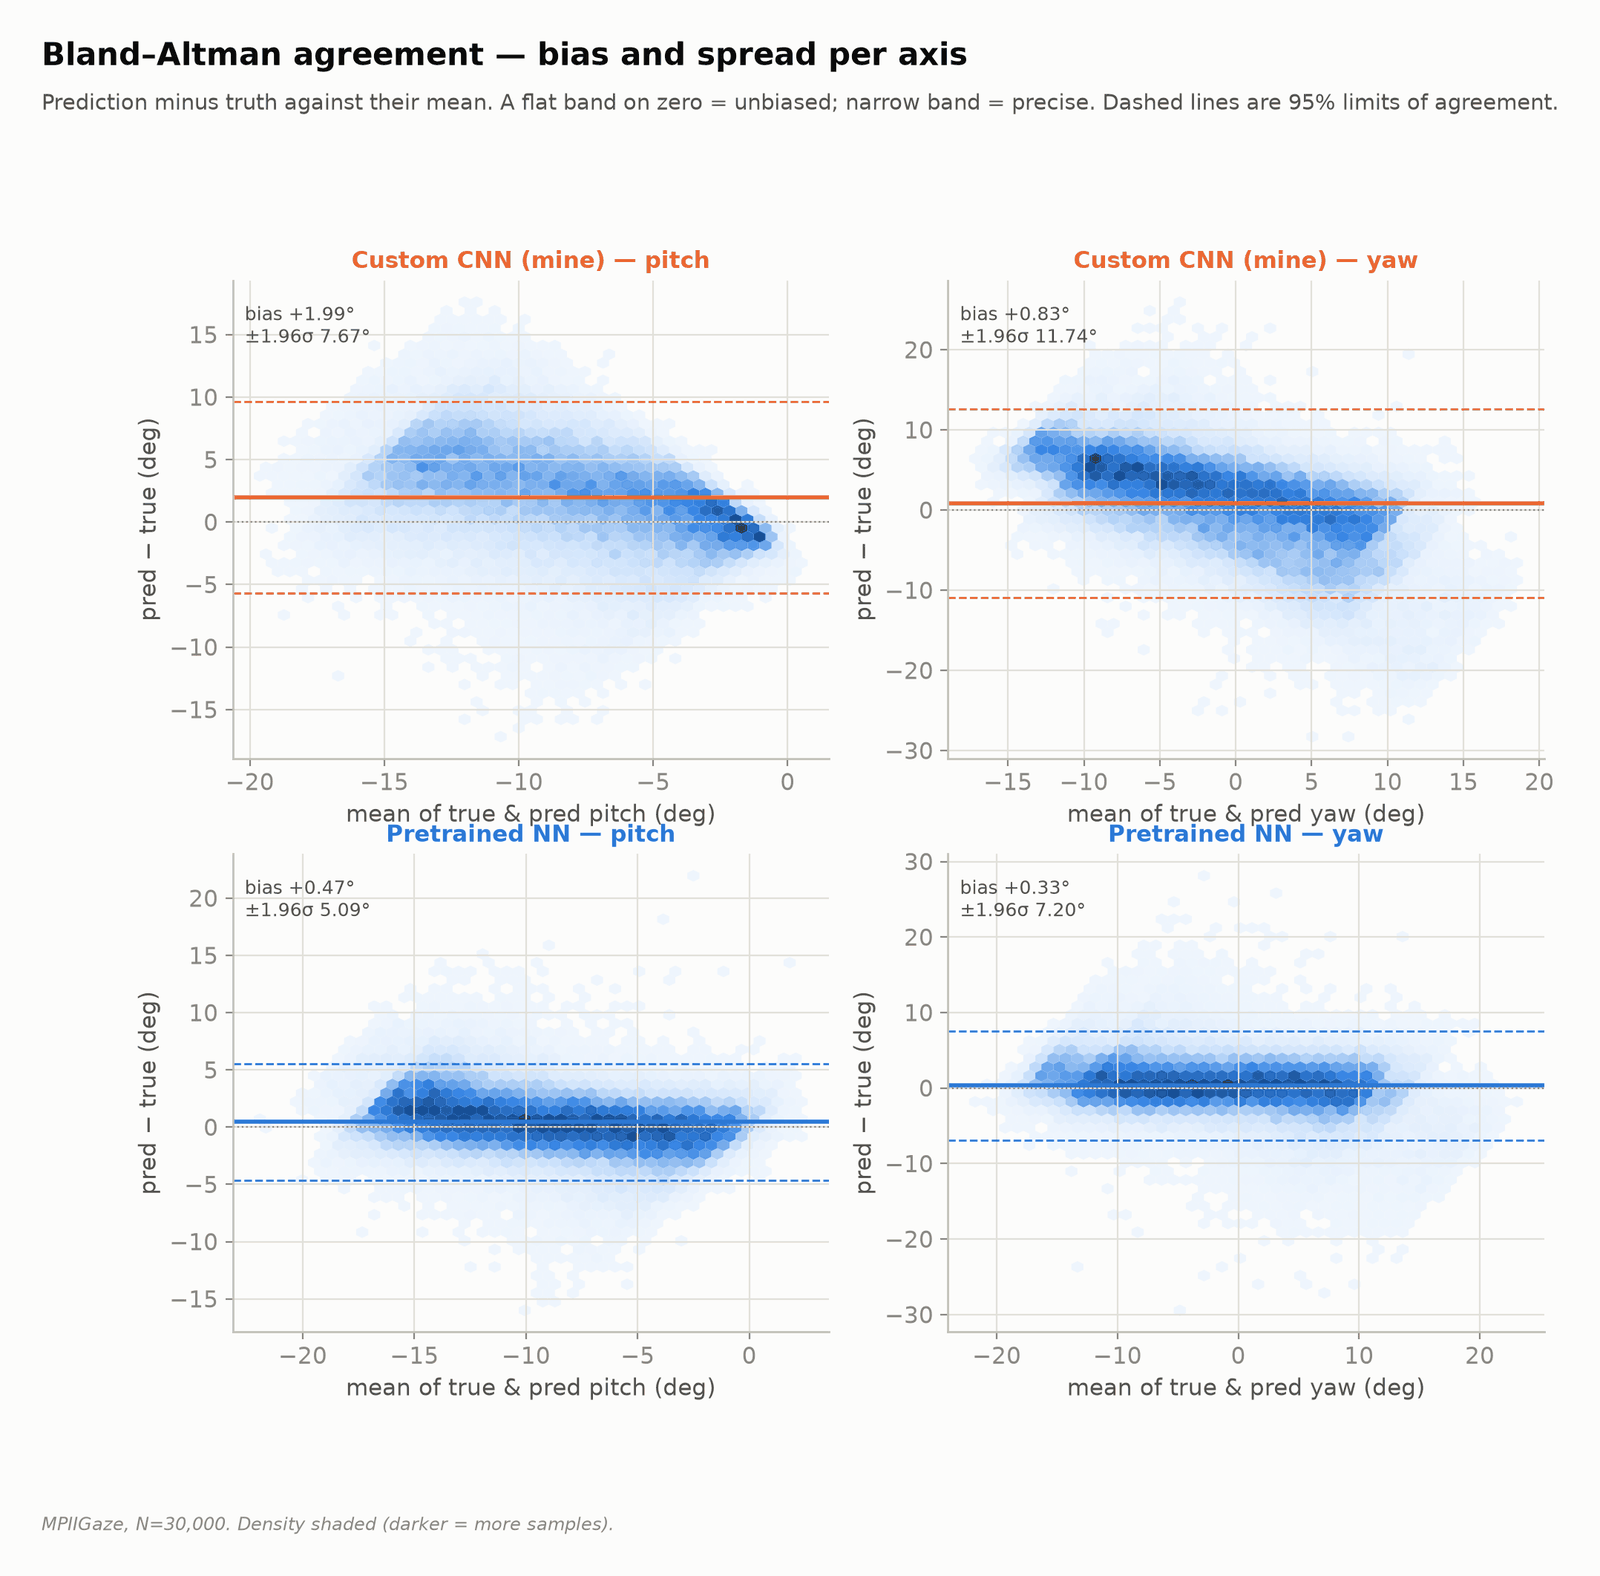
\includegraphics[width=\linewidth]{figures/gaze_G5_bland_altman.png}
\caption{Bland--Altman density --- per-axis bias and 95 \% limits of agreement against ground truth, over a sample-density field.}
\label{fig:8}
\end{figure}

Limits of agreement, defined as

\begin{equation}
\label{eq:206}
\text{LoA}\;_a = \;\text{bias}\;_a \pm 1.96 \cdot \sigma _a ,
\end{equation}

bound 95 \% of individual predictions and are what the cursor controller must absorb:

\begin{equation}
\label{eq:207}
\begin{aligned}
\text{LoA}\;_{\mathrm{pitch}}^A \approx [ -5.68^{\circ}, +9.66^{\circ} ] , \\
\;\text{LoA}\;_{\mathrm{yaw}}^A \approx [ -10.91^{\circ}, +12.57^{\circ} ] ,
\end{aligned}
\end{equation}

\begin{equation}
\label{eq:208}
\begin{aligned}
\text{LoA}\;_{\mathrm{pitch}}^R \approx [ -4.62^{\circ}, +5.56^{\circ} ] , \\
\;\text{LoA}\;_{\mathrm{yaw}}^R \approx [ -6.87^{\circ}, +7.54^{\circ} ] .
\end{aligned}
\end{equation}

The pitch interval's asymmetry is the additive bias of \FIGREF{5} made visible, and the yaw interval is 1.63$\times$ wider than the baseline's --- on the axis carrying most interaction-relevant motion in a seated user, which is why the deployed one-euro filter is tuned with a low minimum cut-off that trades response speed for steadiness at fixation. Neither density field fans, indicating homoscedasticity:

\begin{equation}
\label{eq:209}
\mathrm{Var}[ \hat{\theta } - \theta | \theta ] \approx \;\text{const in}\; \theta ,
\end{equation}

so a variance-stabilising reparameterisation would not help; the error is a constant multiplicative effect, not a signal-dependent one.

\FIGREF{9} stratifies by eccentricity, the variable shrinkage identifies as governing.

\begin{figure}[pos=htbp]
\centering
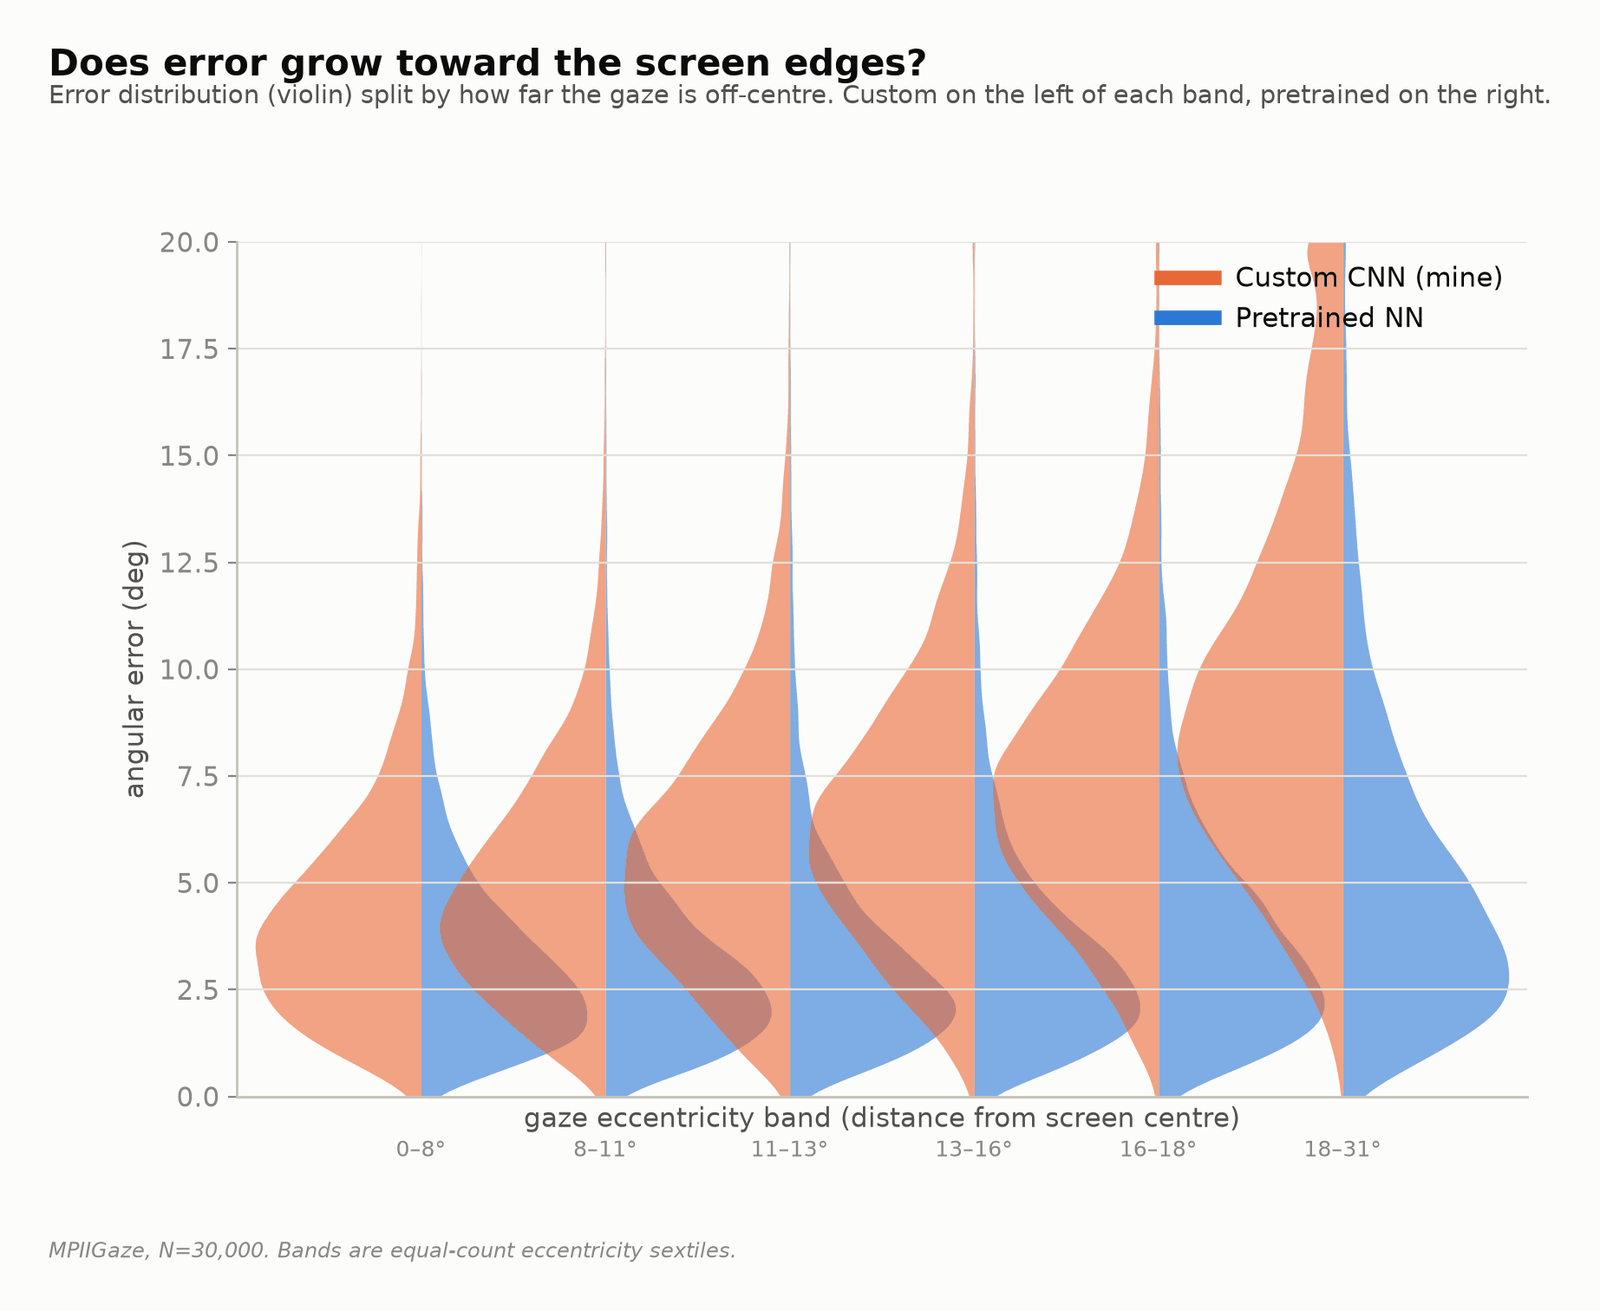
\includegraphics[width=\linewidth]{figures/gaze_G6_eccentricity_ridgeline.png}
\caption{Error versus eccentricity --- angular-error distributions stratified by how far off-centre the true gaze lies.}
\label{fig:9}
\end{figure}

Both models degrade off-axis, which has an optical basis --- foreshortening and eyelid occlusion reduce informative pixels per unit of angular change --- but the ridgelines separate by a broadly constant factor rather than diverging. That distinction discriminates between two accounts. A purely optical limit acts additively on both models,

\begin{equation}
\label{eq:210}
e_M(\|\theta \|) = e_M(0) + \kappa _{\mathrm{opt}}(\|\theta \|) \implies e_A - e_R \;\text{constant in}\; \|\theta \| ,
\end{equation}

whereas a gain deficit acts multiplicatively by \EQREF{194},

\begin{equation}
\label{eq:211}
e_M(\|\theta \|) \approx ( 1 - s_M ) \|\theta \| + \nu _M \implies e_A / e_R \;\text{approximately constant in}\; \|\theta \| .
\end{equation}

The data support \EQREF{211}, so the proposed network has no peripheral failure mode to repair --- only a uniformly contracted response, which is good news for the screen-edge behaviour the deployed 1.2 expansion factor is designed to reach.

\FIGREF{10} exposes the axis asymmetry that pooled error conceals.

\begin{figure}[pos=htbp]
\centering
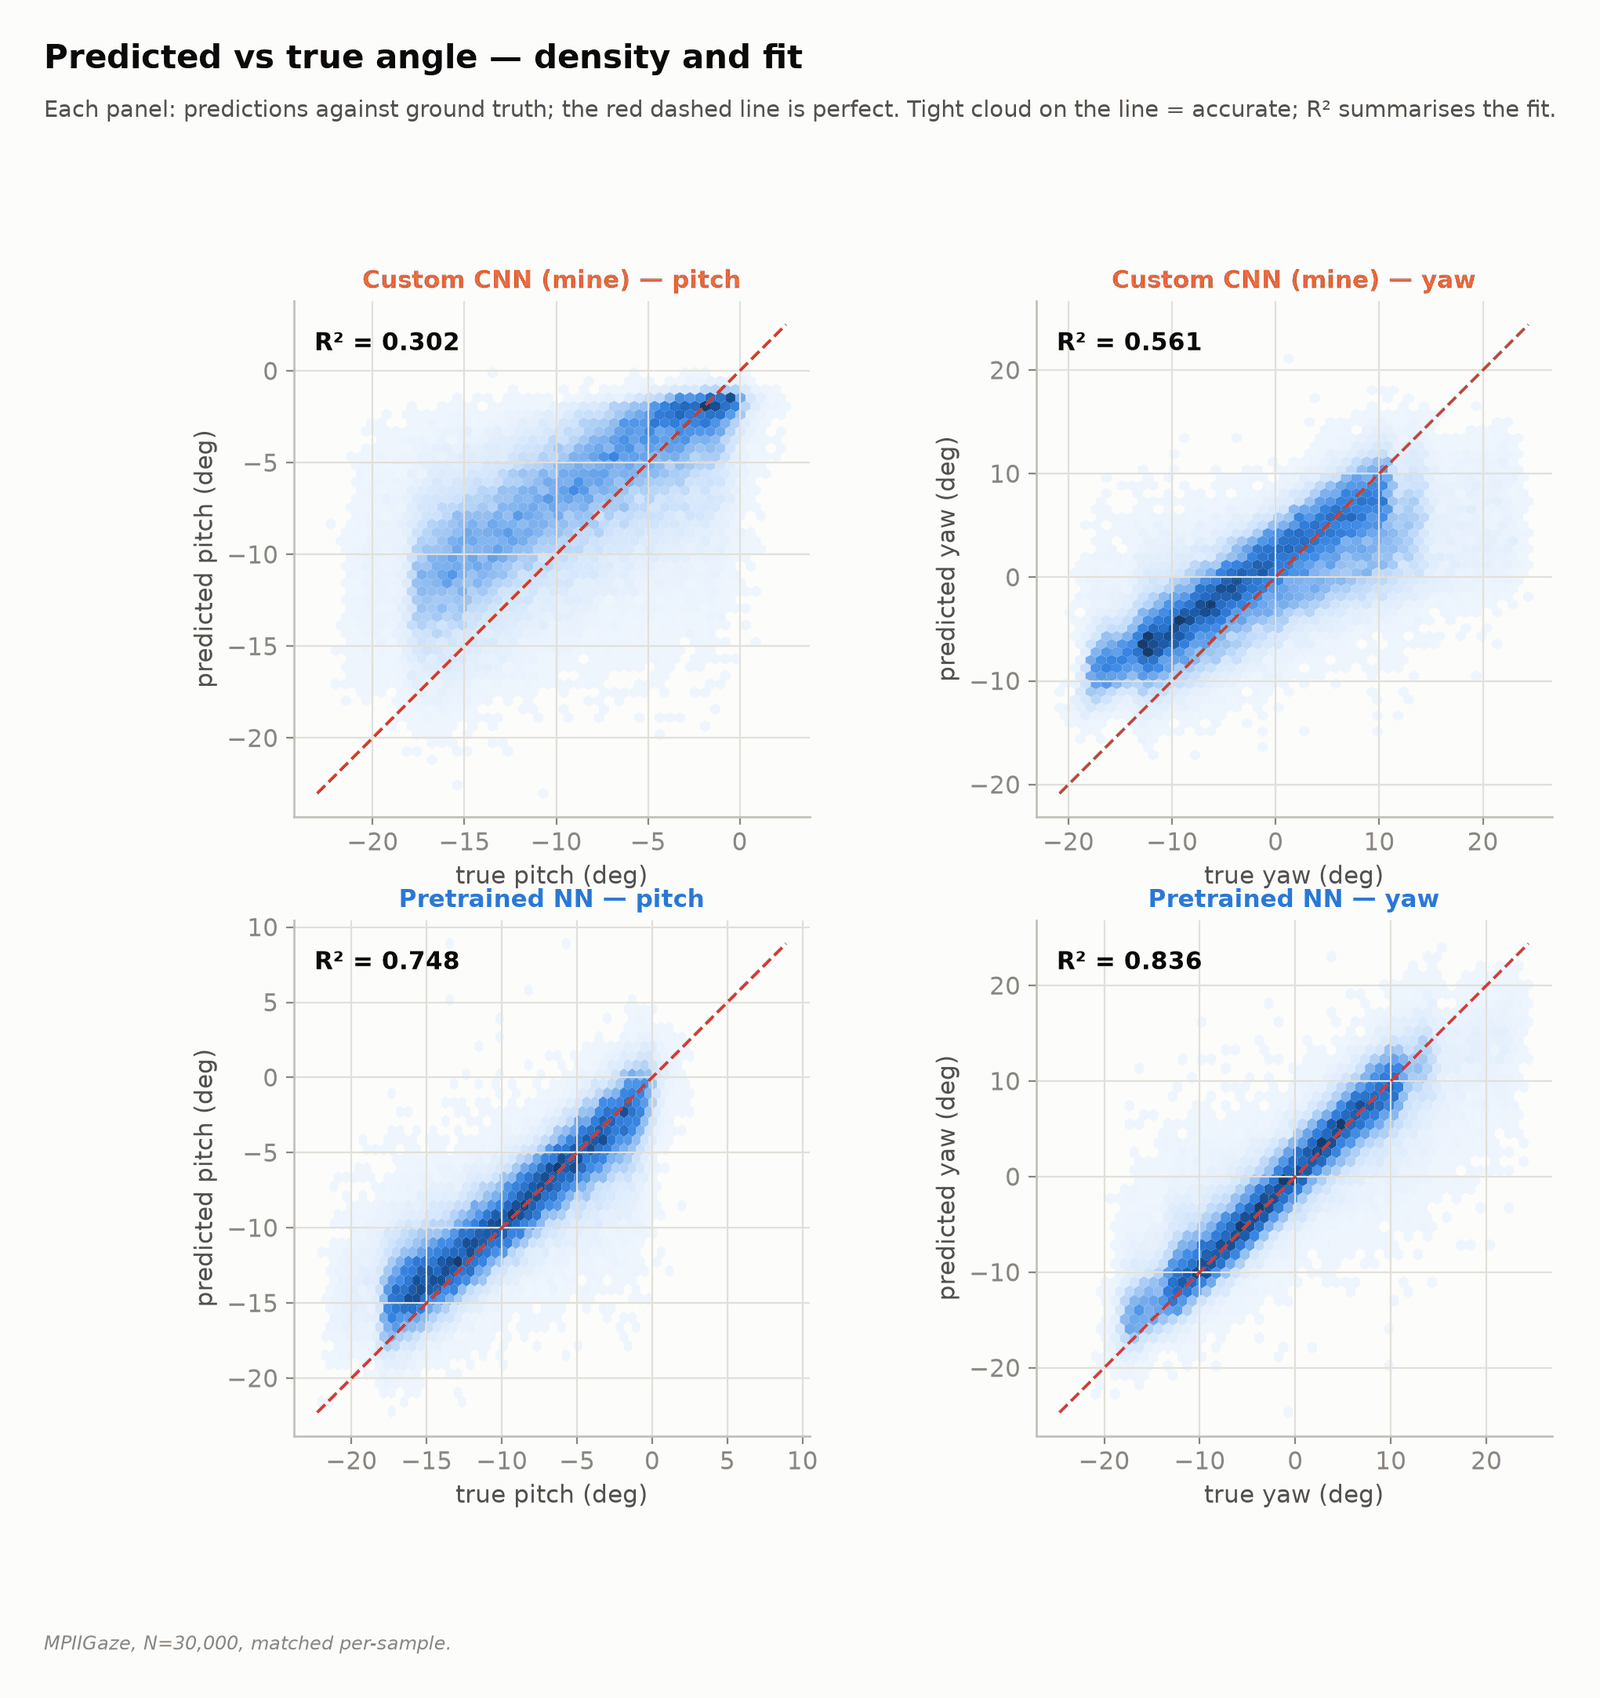
\includegraphics[width=\linewidth]{figures/gaze_G7_true_vs_pred.png}
\caption{Predicted versus true --- density-weighted regression fits with coefficient of determination for pitch and yaw.}
\label{fig:10}
\end{figure}

By \EQREF{153} the proposed network attains R$^{2}$ = 0.302 in pitch and 0.561 in yaw against 0.748 and 0.836. Because its fitted gain is essentially identical on both axes by \EQREF{191}, the R$^{2}$ disparity cannot be a gain effect. Writing \EQREF{153} in terms of the shrinkage model,

\begin{equation}
\label{eq:212}
R^{2}_a = \hat{s}_a^{2} \sigma _{\theta _a}^{2} / ( \hat{s}_a^{2} \sigma _{\theta _a}^{2} + \sigma _{\zeta _a}^{2} ) ,
\end{equation}

equal $\hat{s}_{a}$ on both axes forces the disparity into the residual variance $\sigma_{\zeta^{2}}$. The physical explanation is direct: vertical gaze is signalled through eyelid aperture and iris occlusion, cues confounded with blink state and individual eyelid morphology, whereas horizontal gaze produces a clean identity-invariant lateral translation of the iris. Pitch is thus the axis most contaminated by identity-specific appearance and the one expected to suffer most under a nine-identity training set --- a prediction the attribution analysis of \FIGREF{15} below confirms mechanistically. It also explains why the deployed vertical gain (3.4) is set higher than would be needed for a symmetric estimator.

\FIGRANGE{11}{14} re-render the same per-sample data as continuous fields. They add no measurement, but three of the claims above --- isotropy, the dominance of incoherent over coherent displacement, and residual anisotropy --- are claims about \emph{joint} structure and are tested most directly here.

\begin{figure}[pos=htbp]
\centering
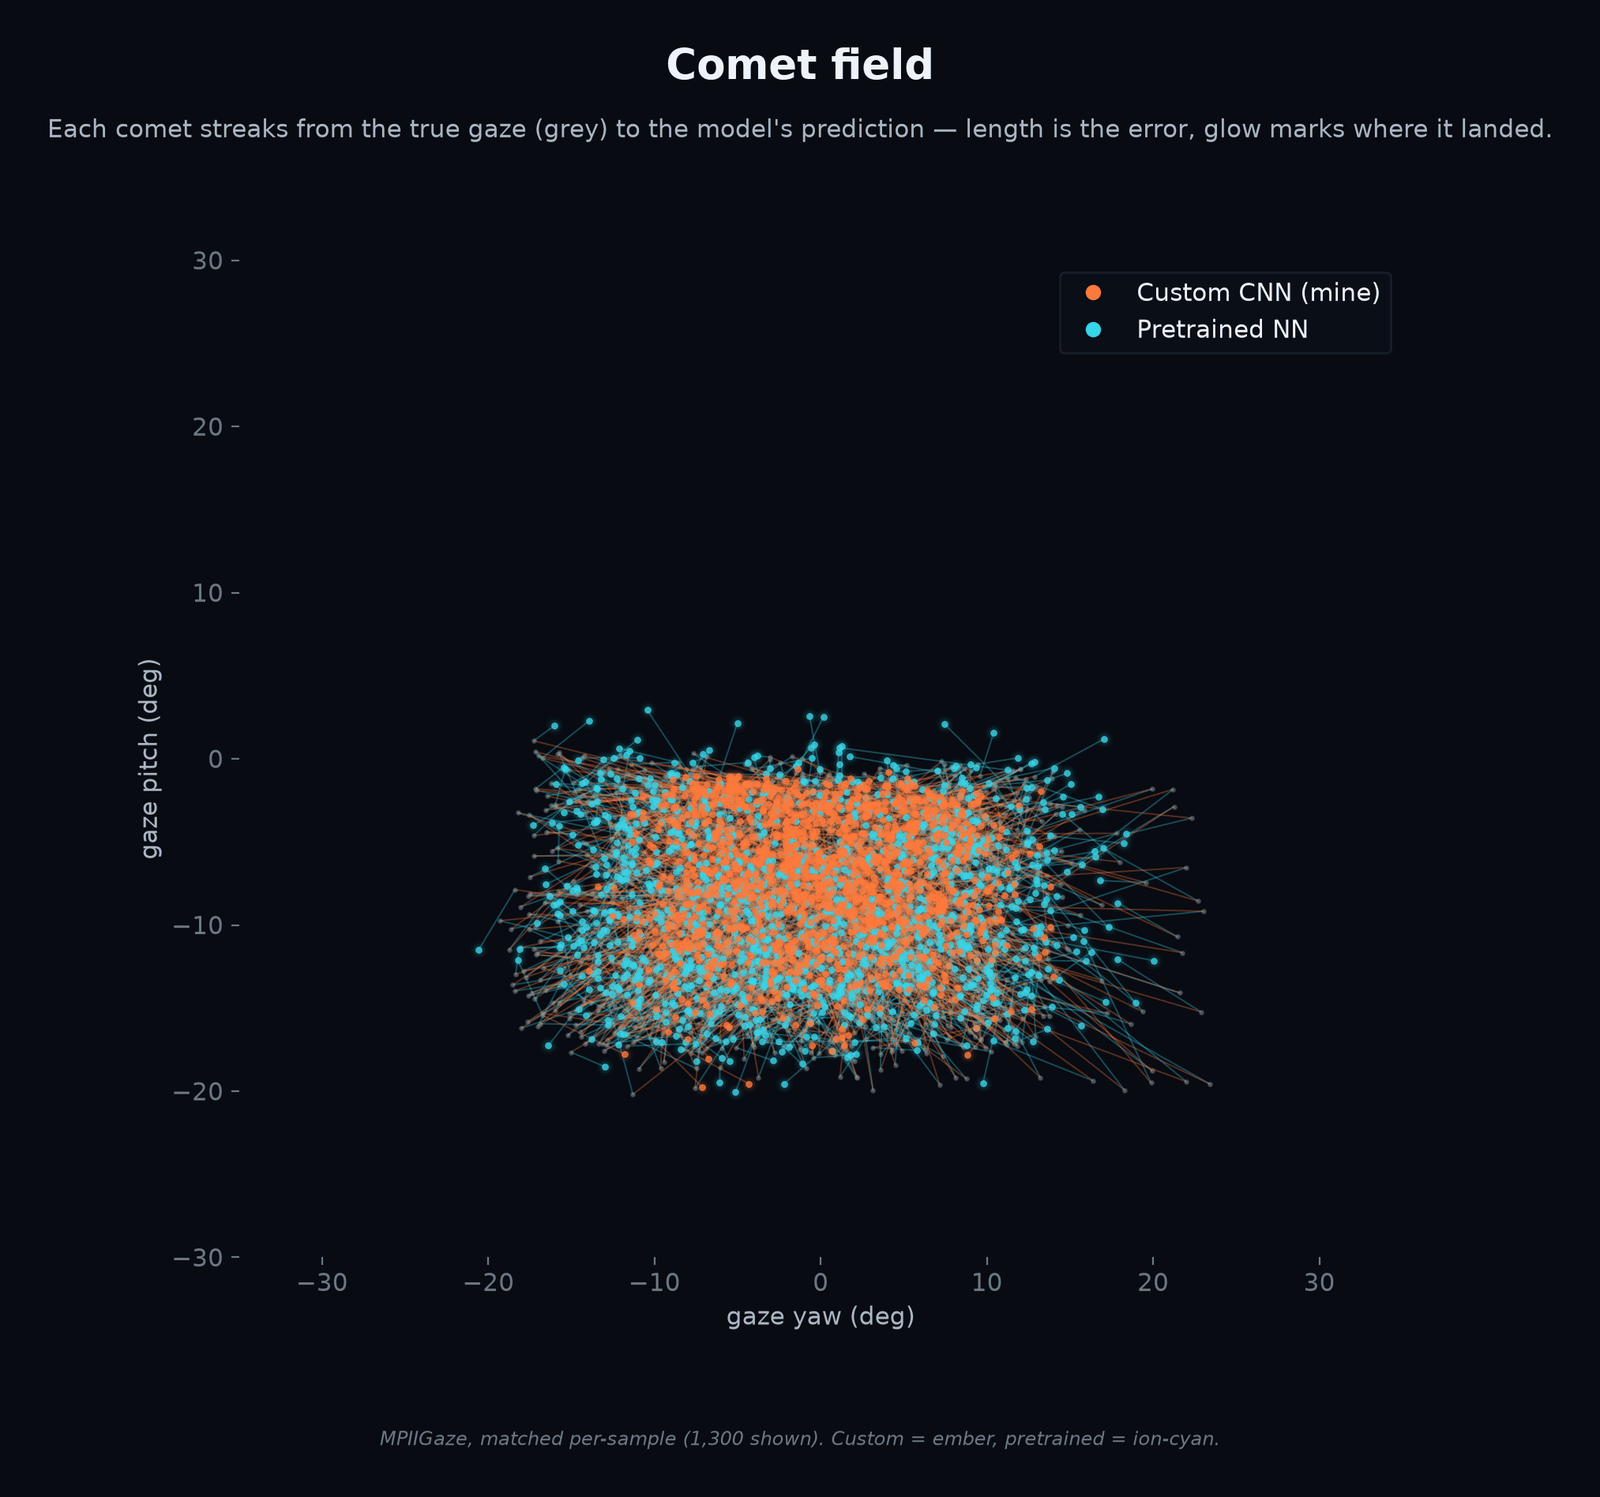
\includegraphics[width=\linewidth]{figures/figures_art_gaze_GA1_comet_field.png}
\caption{Comet field --- every held-out sample drawn as a streak from its true gaze direction to the model's prediction; streak length is the per-sample angular error.}
\label{fig:11}
\end{figure}

Retaining every displacement rather than their mean separates coherent from incoherent error. Decomposing the displacement field,

\begin{equation}
\label{eq:213}
\begin{aligned}
\mathbf{u}(\theta ) = \hat{\theta } - \theta = \mathbb{E}[ \hat{\theta } - \theta | \theta ] + ( \hat{\theta } - \mathbb{E}[ \hat{\theta } | \theta ] ) , \\ 
\text{coherent incoherent}
\end{aligned}
\end{equation}

the streaks share a common upward coherent component of 1.987$^{\circ}$ but their residual directions are largely uncorrelated. Coherent displacement is calibration error and is removable by the deployed polynomial; incoherent displacement is representational noise and is not, passing instead to the one-euro filter. The visual dominance of the incoherent component is the geometric reason exact bias removal recovers only 6.5 \% by \EQREF{196}, and it predicts that most of the deployed system's gaze quality is bought by temporal smoothing rather than by calibration.

\begin{figure}[pos=htbp]
\centering
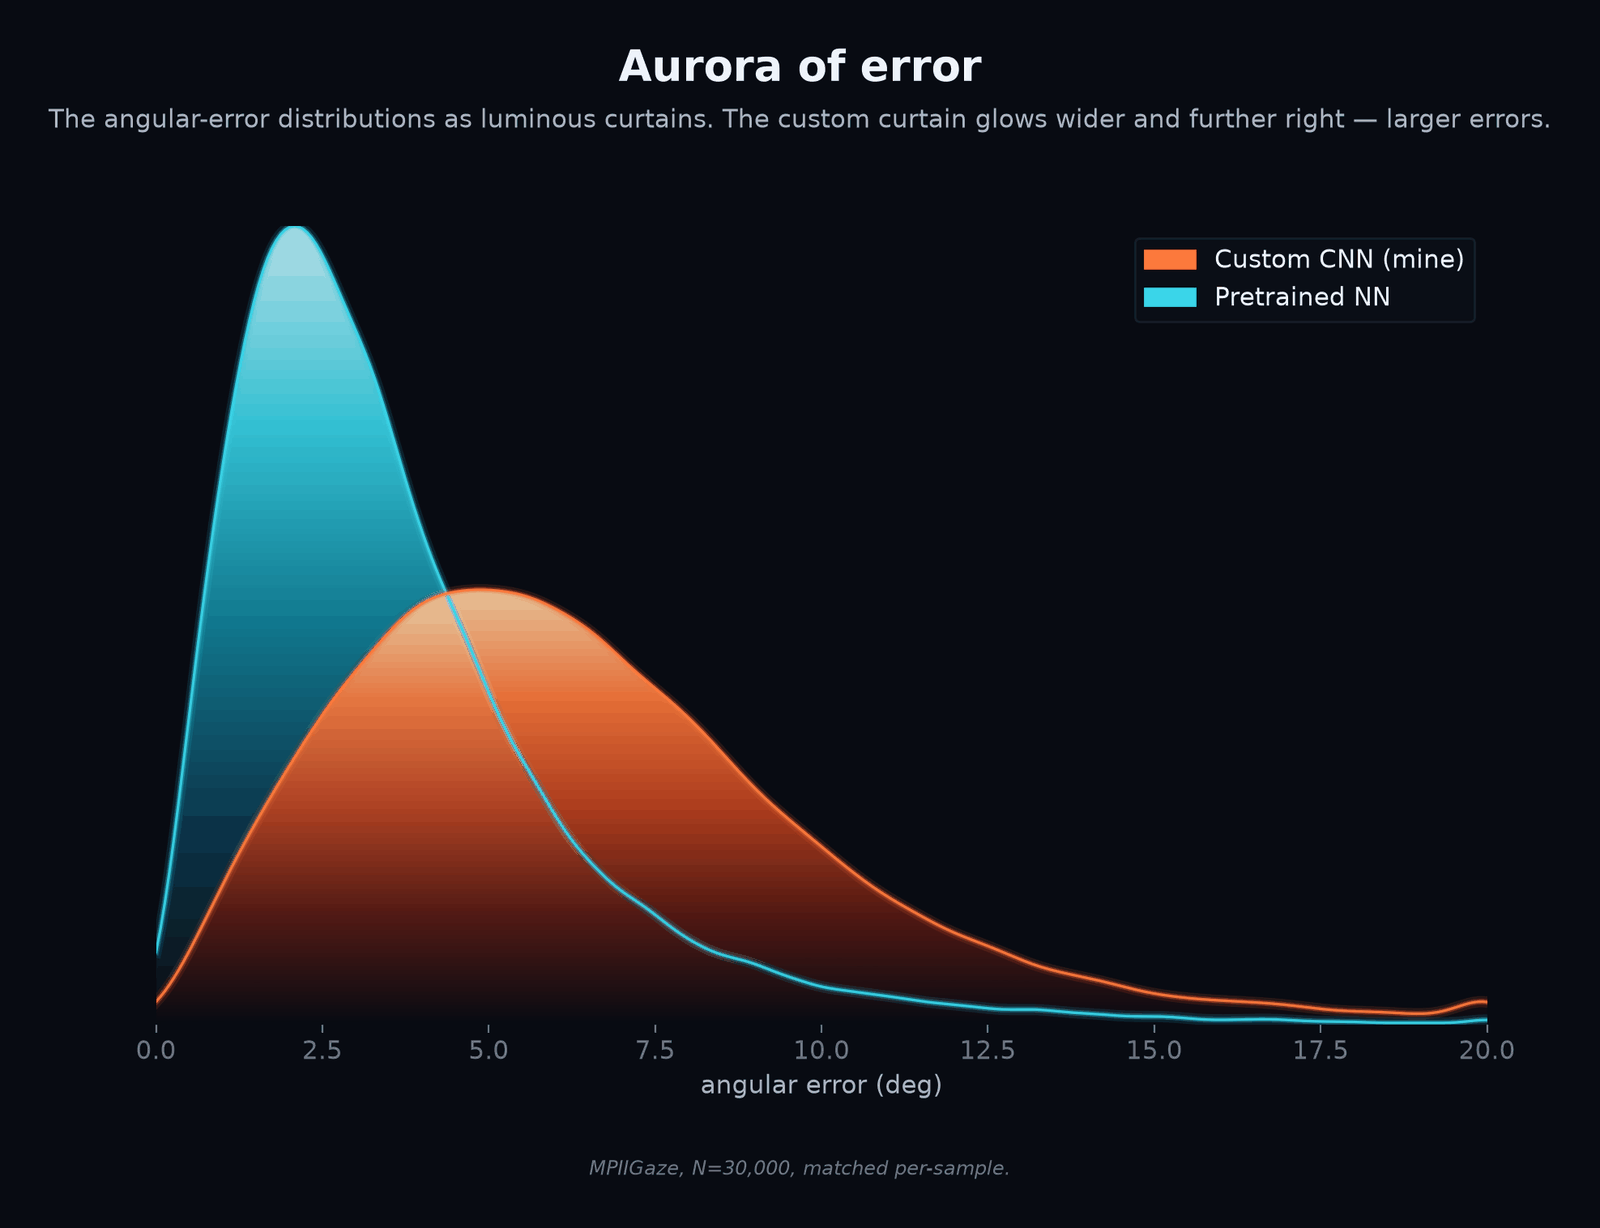
\includegraphics[width=\linewidth]{figures/figures_art_gaze_GA2_aurora.png}
\caption{Aurora of error --- the angular-error distributions of both models rendered as luminous density curtains.}
\label{fig:12}
\end{figure}

The curtains overlap substantially despite a 2.818$^{\circ}$ mean separation --- the graphical form of d = 0.854, large but far from disjoint, and consistent with the 18.86 \% win rate. Both distributions are right-skewed (means 6.439$^{\circ}$ and 3.621$^{\circ}$ against medians 5.873$^{\circ}$ and 2.985$^{\circ}$), with skew ratios

\begin{equation}
\label{eq:214}
\mathrm{mean}/\mathrm{median}: 6.439/5.873 = 1.096 (A) , 3.621/2.985 = 1.213 (R) ,
\end{equation}

so neither model's typical behaviour is captured by its mean, and median-based reporting is the safer convention for this task. The skew is proportionally greater for the baseline, indicating its advantage is realised most strongly on the bulk of easy samples --- precisely where a correctly-scaled estimator gains over a contracted one, since by \EQREF{194} the contracted estimator's systematic error vanishes only at $\theta$ = 0.

\begin{figure}[pos=htbp]
\centering
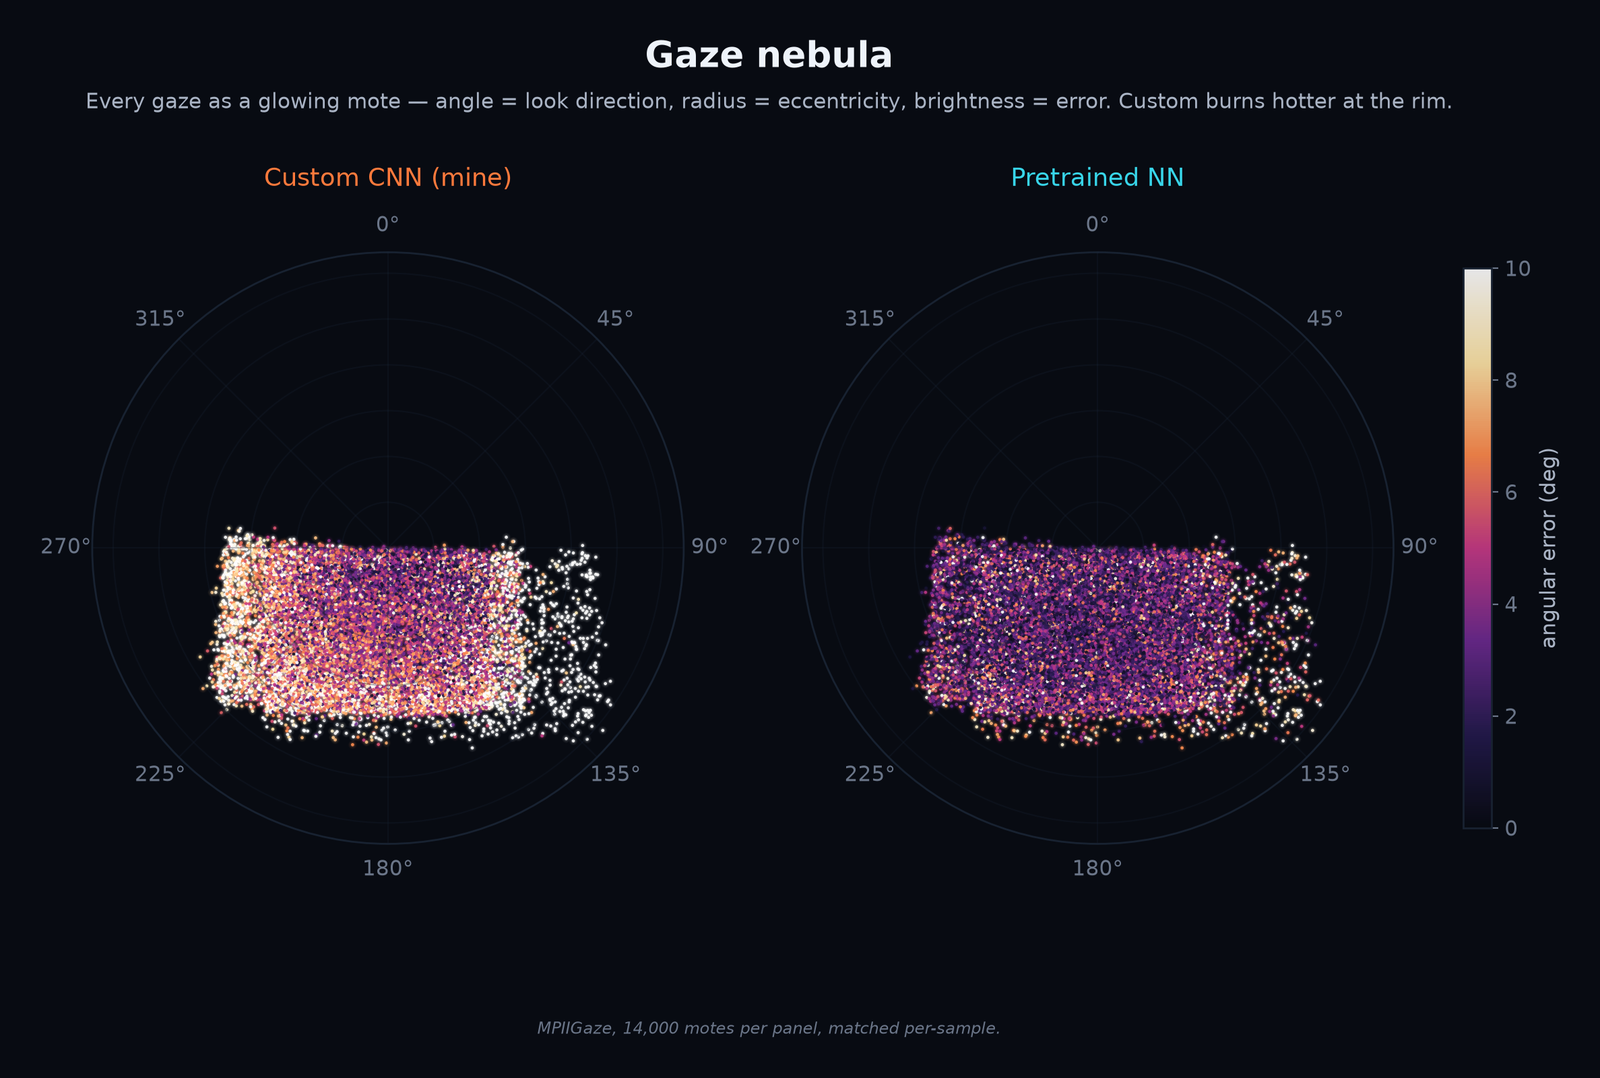
\includegraphics[width=\linewidth]{figures/figures_art_gaze_GA3_nebula.png}
\caption{Gaze nebula --- every held-out gaze as a point placed by direction and eccentricity, with brightness encoding its error.}
\label{fig:13}
\end{figure}

Collapsing the stratifications of Figs. 4 and 8 into one field makes the governing law testable rather than inferred: brightness rises with radius and is uniform in angle. Error is a function of eccentricity alone with no azimuthal dependence --- the exact signature of the (1 -- s)$\|\theta\|$ term of \EQREF{194} and the single strongest confirmation that the gaze deficit is a resolution limit rather than a geometric fault, since any crop or normalisation error would introduce azimuthal asymmetry.

\begin{figure}[pos=htbp]
\centering
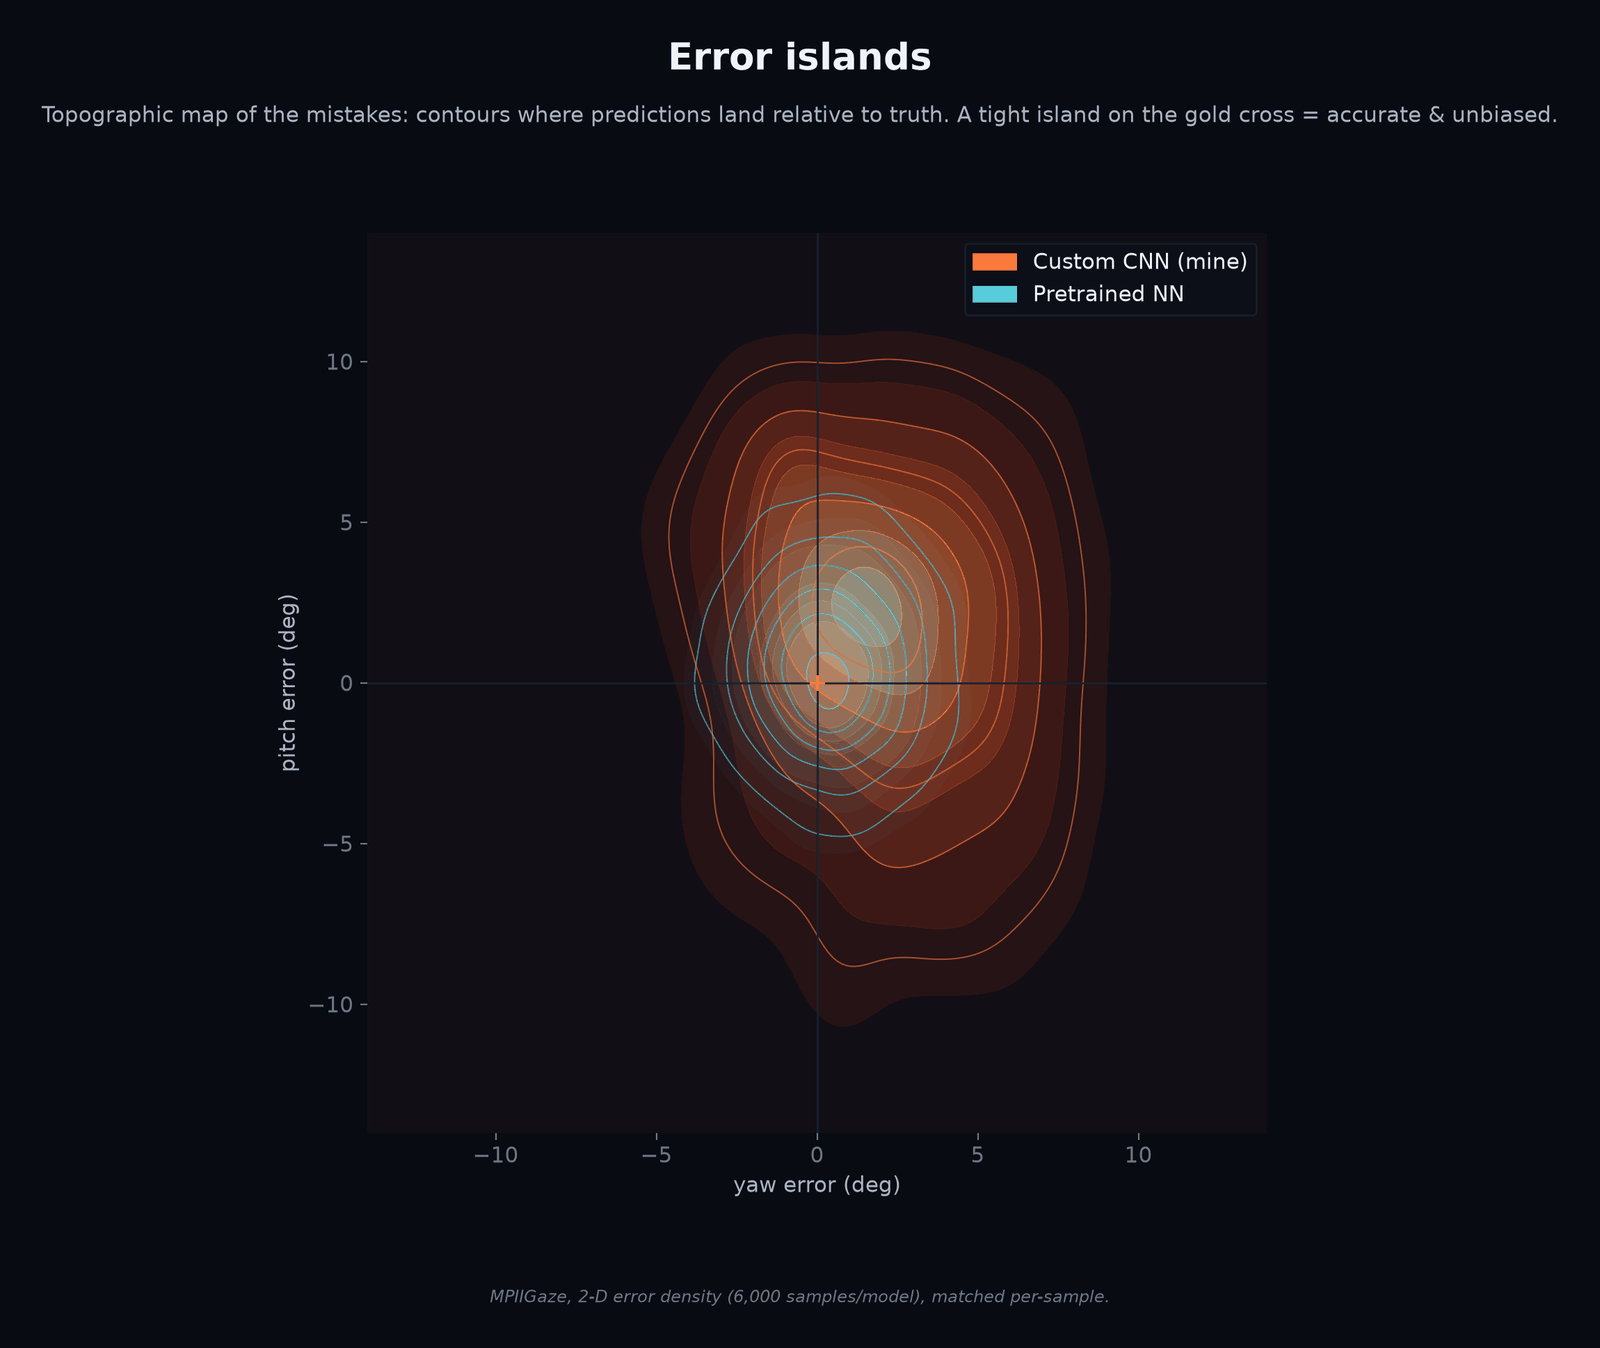
\includegraphics[width=\linewidth]{figures/figures_art_gaze_GA4_error_islands.png}
\caption{Error islands --- density contours of predictions relative to ground truth for each model; a tight island centred on the cross is accurate and unbiased.}
\label{fig:14}
\end{figure}

The proposed network's island is displaced by the 1.987$^{\circ}$ pitch offset and elongated in yaw at a standard-deviation ratio

\begin{equation}
\label{eq:215}
\begin{aligned}
\sigma _{\mathrm{yaw}}/\sigma _{\mathrm{pitch}} = 5.988/3.914 = 1.53 (A) , \\
3.675/2.596 = 1.42 (R) .
\end{aligned}
\end{equation}

The anisotropy is therefore partly intrinsic to the task and partly amplified by the proposed network --- consistent with the horizontally-tuned operator identified next, since an operator optimised for horizontal displacement necessarily places its widest residual along the horizontal axis, and consistent in turn with the deployed controller using different horizontal and vertical gains.

\subsubsection{What the network computes}

Accuracy establishes that a network is right; it does not establish that it is right for a transferable reason. Attribution follows Section 3.10: Integrated Gradients \CITE{ig} against a zero baseline over 32 steps, computed directly on the deployed TorchScript module, with the input partitioned into a 4 $\times$ 4 grid by \EQREF{139} so that each region assumes the role of a feature. Completeness \EQREF{138} makes the decompositions exact rather than indicative.

\begin{figure}[pos=htbp]
\centering
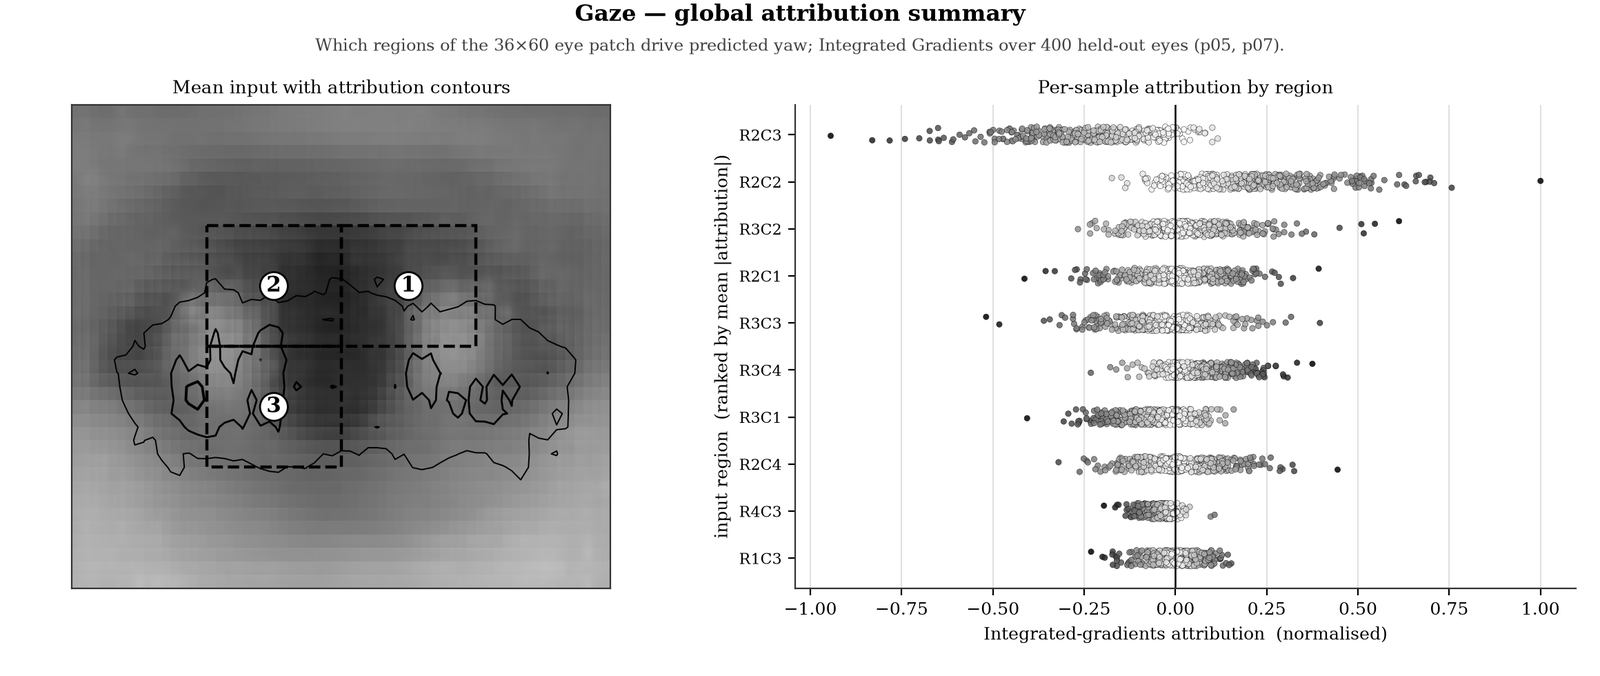
\includegraphics[width=\linewidth]{figures/attribution_gaze_A1_summary.png}
\caption{Gaze --- global attribution summary for predicted yaw over the 36 $\times$ 60 eye patch, regions ranked by mean absolute attribution.}
\label{fig:15}
\end{figure}

The two dominant regions, R2C3 and R2C2, sit side by side across the vertical midline carrying opposite-signed attribution. The network has therefore learned a \textbf{signed differential operator} across the midline,

\begin{equation}
\label{eq:216}
\begin{aligned}
F_{\mathrm{yaw}}(x) \approx \Sigma _{k \in \;\text{left}} w_k \langle x, \\
\phi _k\rangle - \Sigma _{k \in \;\text{right}} w_k \langle x, \phi _k\rangle , \\
w_k > 0 ,
\end{aligned}
\end{equation}

which is exactly the computation yaw estimation requires, since horizontal gaze is encoded by iris displacement relative to the eye-corner frame. Attribution concentrates in the horizontal band with little vertical structure, independently explaining the axis asymmetry of \FIGREF{10}: capacity was allocated horizontally, so pitch is served by whatever vertical signal survives incidentally. That the operator is \emph{differential} rather than absolute is what makes it robust to the illumination variation a home webcam delivers, since a differential operator annihilates the additive component of the photometric family that \EQREF{15} normalises.

\begin{figure}[pos=htbp]
\centering
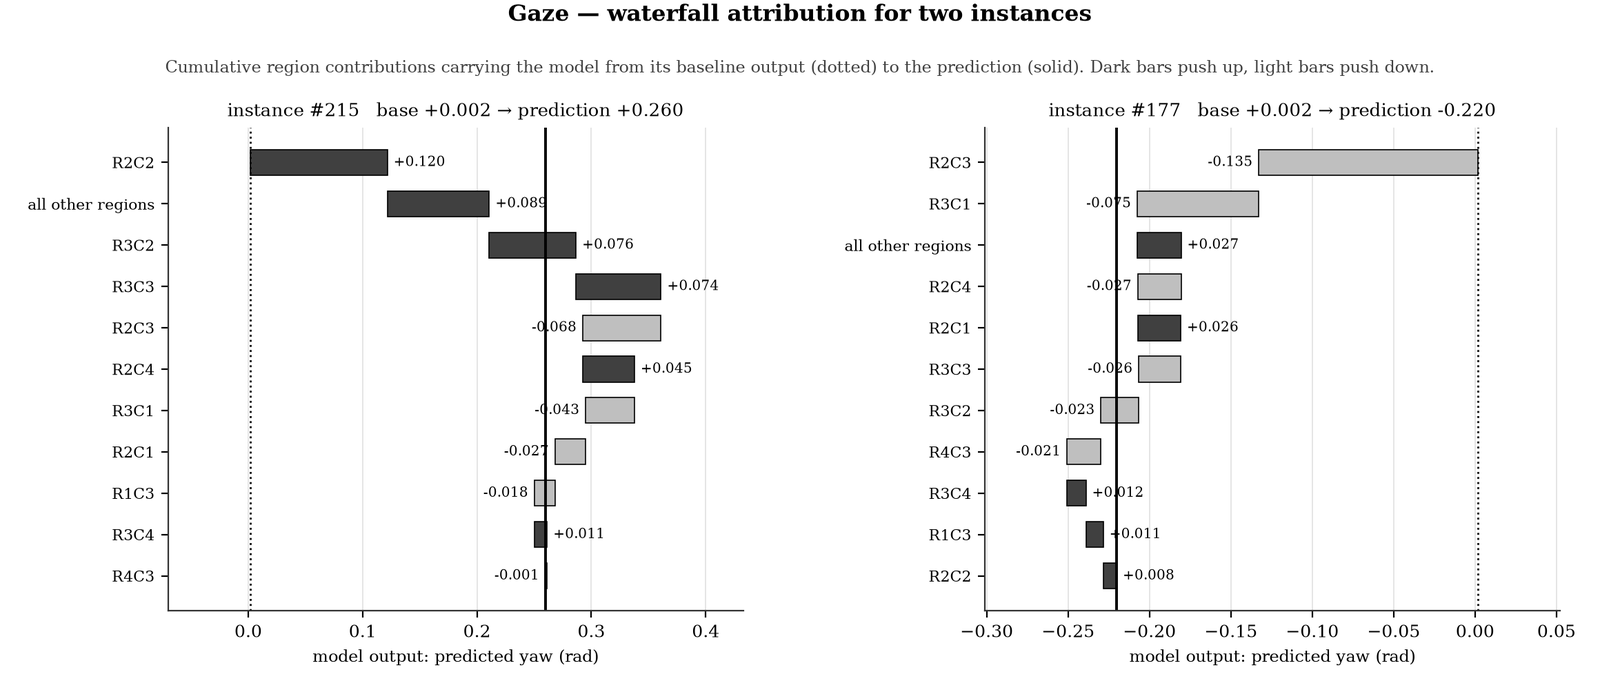
\includegraphics[width=\linewidth]{figures/attribution_gaze_A2_waterfall.png}
\caption{Gaze --- waterfall attribution for two extreme instances of predicted yaw.}
\label{fig:16}
\end{figure}

Extreme instances are carried to their predictions by opposing contributions from the same midline pair, confirming the differential structure operates per instance rather than emerging from averaging. The residual regions contribute a small consistently-signed offset --- the attribution-space counterpart of the +1.987$^{\circ}$ bias of \FIGREF{5} --- which localises that bias in a distributed background term rather than in the discriminative operator, and explains why removing it recovers only 6.5 \% of angular error.

\begin{figure}[pos=htbp]
\centering
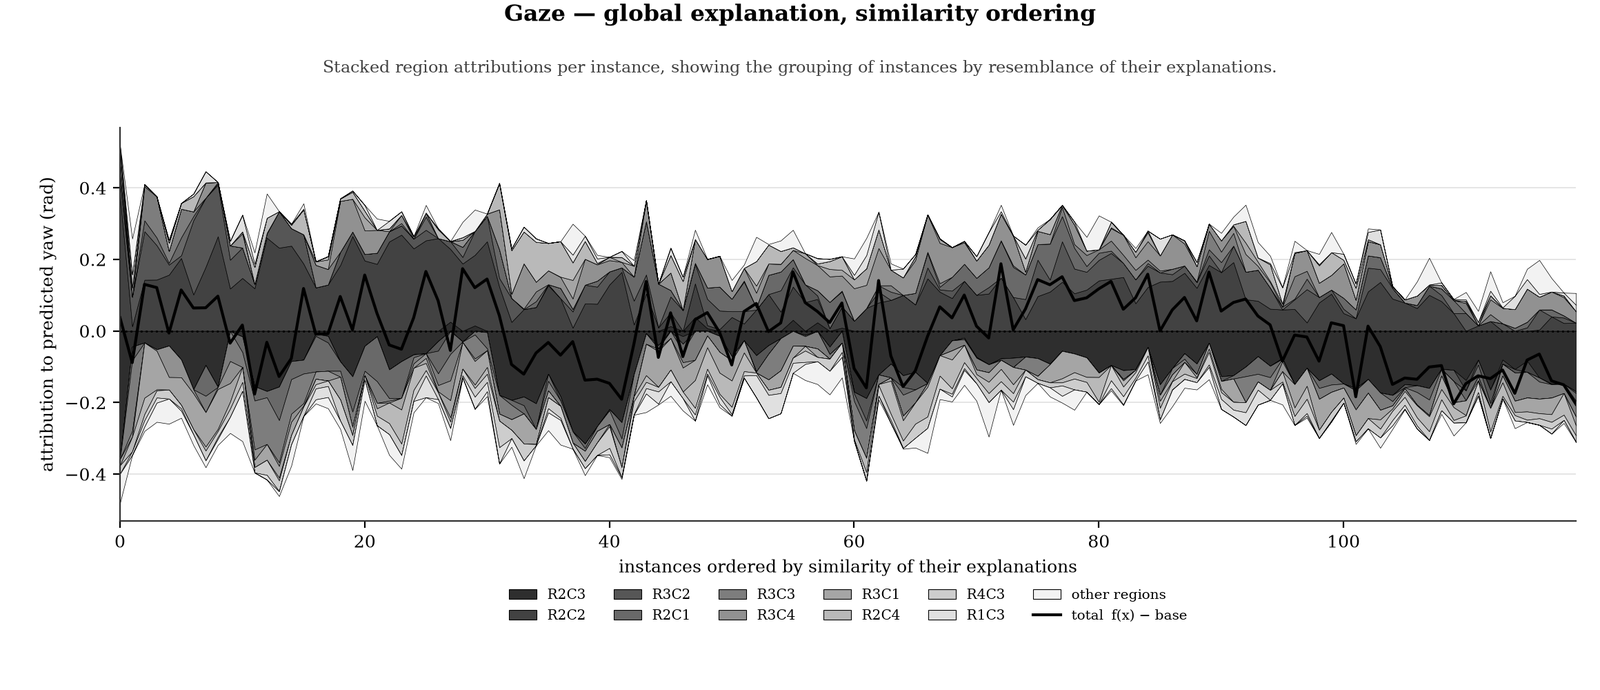
\includegraphics[width=\linewidth]{figures/attribution_gaze_A3_similarity.png}
\caption{Gaze --- global explanation under similarity ordering.}
\label{fig:17}
\end{figure}

Similarity ordering produces a smooth continuum rather than discrete blocks, which is correct for regression over a continuous target: neighbouring gaze angles should induce neighbouring explanations. Formally, the explanation map is approximately Lipschitz,

\begin{equation}
\label{eq:217}
\| \mathrm{Attr}(\cdot ; x_{1}) - \mathrm{Attr}(\cdot ; x_{2}) \| \leq L \| \theta (x_{1}) - \theta (x_{2}) \| ,
\end{equation}

with no discontinuity anywhere along the ordering. This rules out piecewise or identity-conditioned strategy switching, so the elevated error of Section 5.2.2 is uniform representational imprecision rather than a mixture of a good rule and a bad one --- the attribution-level statement of the isotropic error field of \FIGREF{4}, reached by an independent route.

\begin{figure}[pos=htbp]
\centering
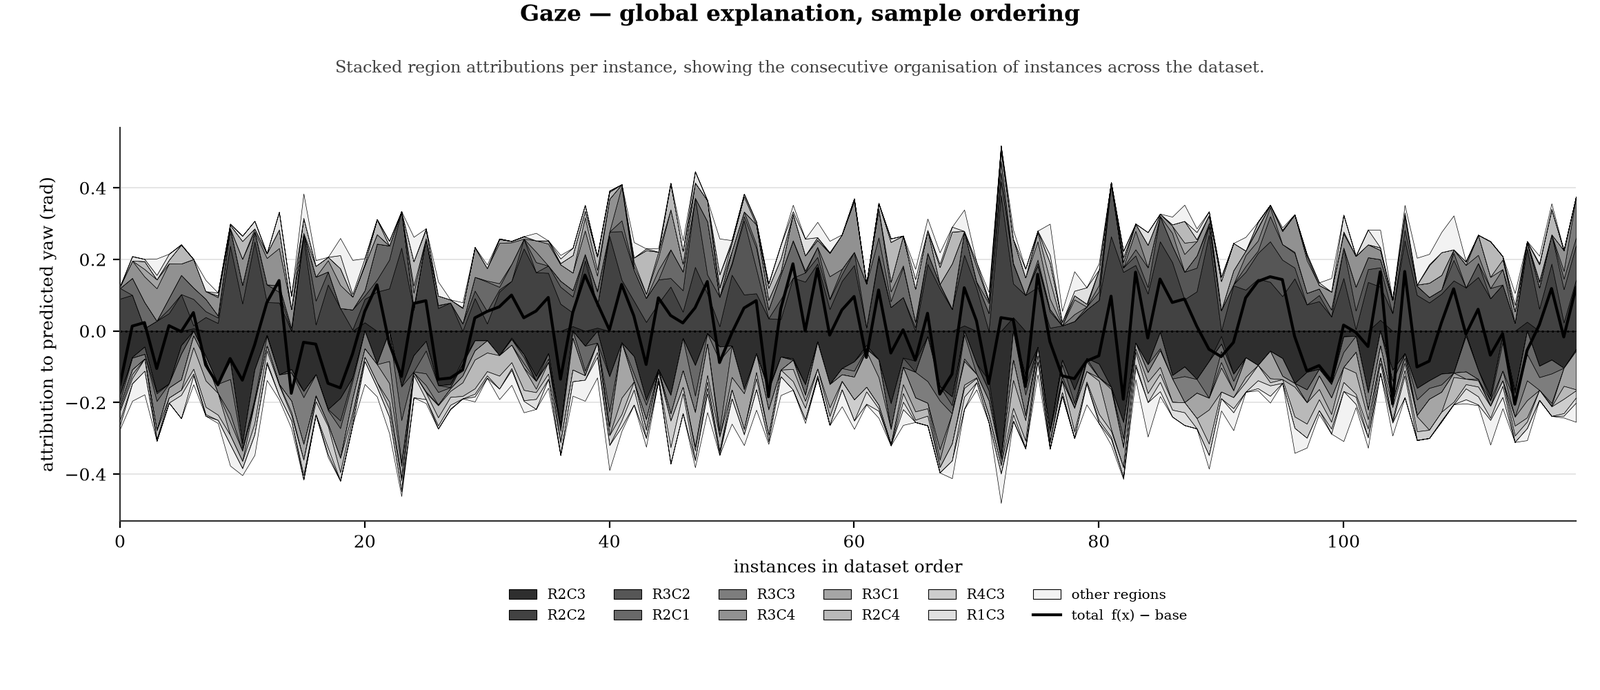
\includegraphics[width=\linewidth]{figures/attribution_gaze_A4_ordering.png}
\caption{Gaze --- global explanation under dataset ordering across held-out participants p05 and p07.}
\label{fig:18}
\end{figure}

Explanation structure stays coherent across the participant boundary while accuracy does not:

\begin{equation}
\label{eq:218}
e_{\mathrm{ang}}(p05) = 5.786^{\circ} , e_{\mathrm{ang}}(p07) = 7.138^{\circ} ,
\end{equation}

\begin{equation}
\label{eq:219}
\begin{aligned}
( \hat{s}_{\mathrm{pitch}}, \hat{s}_{\mathrm{yaw}} )(p05) = ( 0.586, 0.630 ) , \\
( \hat{s}_{\mathrm{pitch}}, \hat{s}_{\mathrm{yaw}} )(p07) = ( 0.377, 0.430 ) .
\end{aligned}
\end{equation}

The same operator is applied to both at substantially different gain, which localises identity sensitivity in the operator's \emph{calibration} rather than its \emph{form}. Writing the per-participant model as

\begin{equation}
\label{eq:220}
\begin{aligned}
\hat{\theta } = s(g) \cdot \mathcal{O}(x) + c(g) , \\
\mathcal{O} \;\text{fixed across g} , s(g) \;\text{varying} ,
\end{aligned}
\end{equation}

this is the mechanism behind the ceiling established next, and it is also the strongest available justification for the deployed per-user calibration stage: if identity enters as a scalar gain, a per-user scalar fit is the structurally correct remedy, and \EQREF{106}--\EQREF{107} is exactly such a fit.

\subsubsection{The ceiling is set by identity count, not sample count}

To test whether the residual error was data-limited, the network was retrained on 250,000 samples (175,199 training frames, 3.1$\times$ the configuration of Section 5.2.1). Validation error did not improve:

\begin{equation}
\label{eq:221}
6.32^{\circ} at 3.1\times \;\text{data}\; \mathrm{against} 5.81^{\circ} at 1\times ,
\end{equation}

a null result --- indeed a slight regression within run-to-run variation. The explanation follows directly from the effective-sample-size relation \EQREF{10}. Additional frames from the same nine identities are strongly correlated with those already present, so they raise n but not G, and by \EQREF{10}

\begin{equation}
\label{eq:222}
n_{\mathrm{eff}} = n / [ 1 + (\bar{n} - 1) \rho ] \to G / \rho as \bar{n} \to \infty ,
\end{equation}

which is bounded above by a constant depending only on the identity count. Extra frames therefore tighten the empirical risk estimate without enlarging the set of appearance modes the hypothesis must cover. \FIGREF{18} supplies the mechanism --- what nine identities fail to span is the \emph{range of gain} s(g) in \EQREF{220}, not the \emph{form} of the operator $\mathcal{O}$ --- and this explains why augmentation succeeded where more data failed: augmentation synthesises new imaging conditions by \EQREF{34}, while further frames of the same nine people supply none.

For the project this converts an open-ended tuning effort into a closed question. No further optimisation on MPIIGaze will close the gap to the pretrained baseline; only a corpus with more participants would, and Section 5.7 therefore recommends adopting the pretrained model rather than continuing to tune. It also predicts that gaze alone among the four modalities would benefit disproportionately from more participants rather than more frames --- a prediction the other three sections test implicitly, since none of them exhibits the same identity--gain coupling.

\FloatBarrier

\subsection{Head pose --- discrete gesture control}

Head pose does not position anything. It fires discrete application and tab gestures through the thresholded state machine of \ALGREF{6}: yaw triggers at 30$^{\circ}$ and releases at 12$^{\circ}$, pitch at 22$^{\circ}$ and 9$^{\circ}$, with a 650 ms dwell ($\approx$20 frames at the configured 30 fps by \EQREF{128}) and a 1,200 ms cooldown. Two consequences follow immediately from \EQREF{124}--\EQREF{129} and govern how the figures below should be read. Absolute mean absolute error is not the governing statistic --- what matters is whether error can carry a pose across a trigger boundary. And because the dwell requirement averages roughly twenty frames, \textbf{bias survives averaging while variance does not}, by \EQREF{129}, which inverts the usual ranking of the two.

Against the 6-D rotation-representation baseline on all 1,969 AFLW2000 faces, both models scoring the identical crop with no preprocessing asymmetry, the proposed network attains 7.367$^{\circ}$ MAE (median 4.185$^{\circ}$) against 3.482$^{\circ}$ (median 1.919$^{\circ}$). The paired statistics are

\begin{equation}
\label{eq:223}
\begin{aligned}
\bar{d} = 3.884^{\circ} \pm 0.272^{\circ} (95 \%) , \;\text{Cohen}\;'s d = 0.632 , \\
\;\text{Wilcoxon p}\; = 1.2 \times 10^{-226} ,
\end{aligned}
\end{equation}

\begin{equation}
\label{eq:224}
\begin{aligned}
\mathbb{P}[ e_A < e_R ] = 14.58 \% , r_{\mathrm{AR}} = 0.671 , \\
\bar{E}_{\mathrm{oracle}} = 3.222^{\circ} , \;\text{Gain}\;_{\mathrm{max}} = 7.5 \% .
\end{aligned}
\end{equation}

The error correlation of 0.671 is \emph{higher} than gaze's 0.491, and the oracle bound correspondingly tighter. Fusion is again unjustified, for the same structural reason: the two models fail on the same faces.

\textbf{The gain measurement transfers, with an instructive asymmetry.} Applying \EQREF{154} axis-wise,

\begin{equation}
\label{eq:225}
\begin{aligned}
\hat{s}_{\mathrm{yaw}}^A = 0.822 , \hat{s}_{\mathrm{pitch}}^A = 0.455 , \\
\hat{s}_{\mathrm{roll}}^A = 0.490 ,
\end{aligned}
\end{equation}

\begin{equation}
\label{eq:226}
\begin{aligned}
\hat{s}_{\mathrm{yaw}}^R = 1.046 , \hat{s}_{\mathrm{pitch}}^R = 0.768 , \\
\hat{s}_{\mathrm{roll}}^R = 0.877 .
\end{aligned}
\end{equation}

Yaw --- by far the widest-support axis in AFLW2000 --- is the only one reproduced at near-correct scale, and the pattern is exactly what the shrinkage account \EQREF{155} predicts. Since s* = $\sigma_{\theta^{2}}$/($\sigma_{\theta^{2}}$ + $\sigma_{\varepsilon^{2}}$), an axis with wide target support has large $\sigma_{\theta^{2}}$ and therefore a gain close to unity at fixed representational noise:

\begin{equation}
\label{eq:227}
\partial s* / \partial \sigma _{\theta} ^{2} = \sigma _{\varepsilon} ^{2} / ( \sigma _{\theta} ^{2} + \sigma _{\varepsilon} ^{2} )^{2} > 0 ,
\end{equation}

so wide target support supplies the gradient signal needed to resist contraction while the two narrow-support axes collapse to approximately half gain --- the same regime as gaze. Inverting \EQREF{158} per axis gives implied noise ratios

\begin{equation}
\label{eq:228}
\begin{aligned}
\hat{\sigma }_{\varepsilon} ^{2}/\sigma _{\theta} ^{2}: 0.217 (\text{yaw}) , \\
1.198 (\text{pitch}) , 1.041 (\text{roll}) ,
\end{aligned}
\end{equation}

confirming that the representation is markedly more informative about yaw than about the other two. That yaw is the best-scaled axis is fortunate for the interface, since yaw carries the two most-used gestures.

\FIGREF{19} begins with the per-axis error structure, which \TABREF{6} identifies as the decisive one.

\begin{figure}[pos=htbp]
\centering
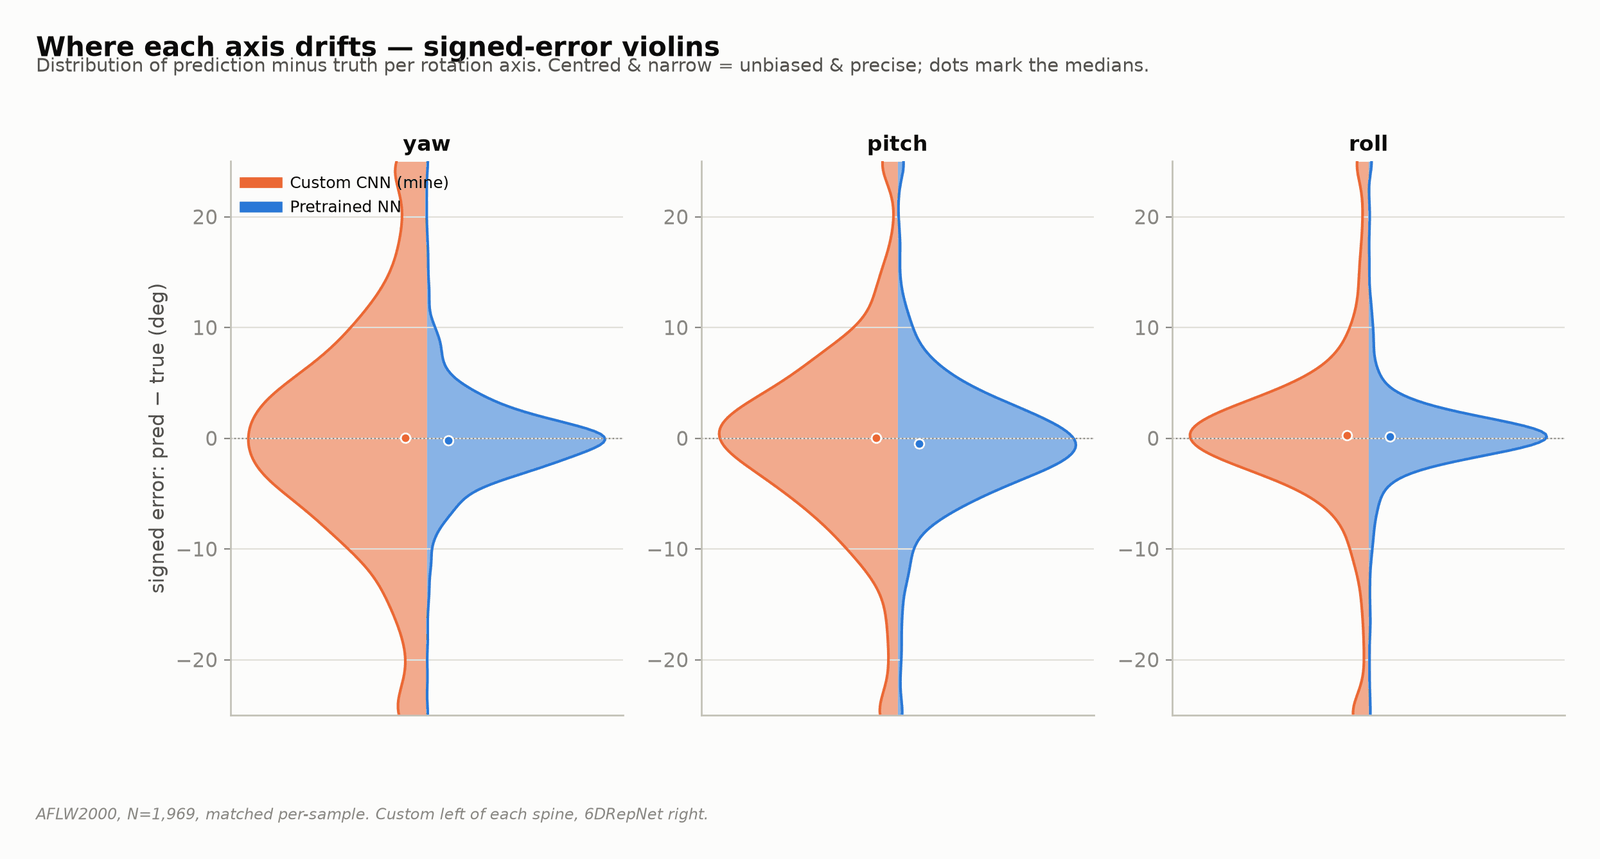
\includegraphics[width=\linewidth]{figures/headpose_H1_signed_violins.png}
\caption{Signed-error violins --- per-axis bias and spread, proposed network left of each spine and 6-D rotation baseline right.}
\label{fig:19}
\end{figure}

All three axes are essentially unbiased. By \EQREF{152},

\begin{equation}
\label{eq:229}
\begin{aligned}
\text{bias}\;^A = ( +0.109^{\circ} , -0.327^{\circ} , +0.062^{\circ} ) , \\
\;\text{bias}\;^R = ( -0.240^{\circ} , -0.624^{\circ} , +0.250^{\circ} ) ,
\end{aligned}
\end{equation}

so the entire deficit is spread, not offset --- the opposite decomposition to gaze, where a 1.987$^{\circ}$ pitch bias was the largest correctable term. This is the single most favourable result for the deployed gesture rule. Substituting the measured yaw spread into \EQREF{129} at the independence limit $\varrho$ = 0,

\begin{equation}
\label{eq:230}
\sigma _{\mathrm{dwell}}^{\mathrm{yaw}} = 12.49^{\circ} / \sqrt{20} = 2.79^{\circ} ,
\end{equation}

comfortably inside the 18$^{\circ}$ hysteresis band between the 30$^{\circ}$ trigger and the 12$^{\circ}$ release. Consecutive frames are correlated, so the true reduction is smaller: at a plausible $\varrho$ = 0.5 the same computation gives

\begin{equation}
\label{eq:231}
\sigma _{\mathrm{dwell}}^{\mathrm{yaw}} = ( 12.49/\sqrt{20} ) \cdot \sqrt{1.5/0.5} = 2.79 \times 1.732 = 4.84^{\circ} ,
\end{equation}

still well inside the band. Equation \EQREF{230} is therefore an upper bound on the benefit and \EQREF{231} a more realistic figure; the direction is unambiguous in either case, and it holds \textbf{only because the bias is near zero}. Had the network carried a gaze-like 2$^{\circ}$ offset, no amount of dwell averaging would have removed it, since \EQREF{129} attenuates only the variance term.

\FIGREF{20} aggregates four error measures across three axes.

\begin{figure}[pos=htbp]
\centering
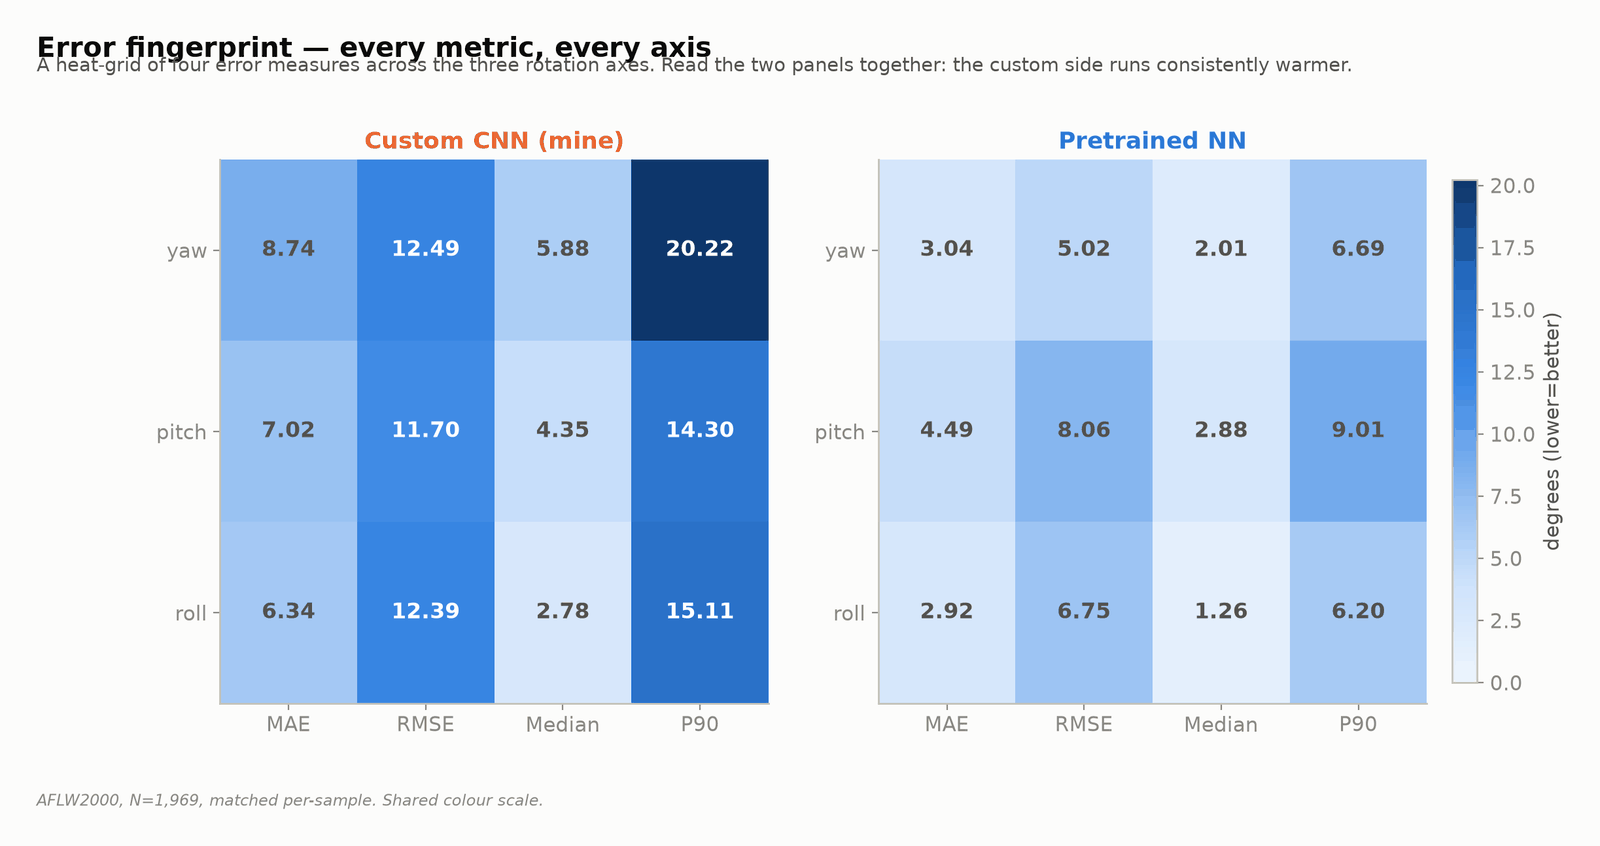
\includegraphics[width=\linewidth]{figures/headpose_H2_fingerprint.png}
\caption{Error fingerprint --- heat grid of four error measures across yaw, pitch and roll for each model.}
\label{fig:20}
\end{figure}

The fingerprint contains an axis-ranking inversion that the gain analysis resolves. The proposed network's MAE ordering is

\begin{equation}
\label{eq:232}
\text{yaw}\; (8.742^{\circ}) > \;\text{pitch}\; (7.023^{\circ}) > \;\text{roll}\; (6.335^{\circ}) ,
\end{equation}

while the baseline's is

\begin{equation}
\label{eq:233}
\text{pitch}\; (4.492^{\circ}) > \;\text{yaw}\; (3.039^{\circ}) > \;\text{roll}\; (2.916^{\circ}) .
\end{equation}

Yaw is simultaneously the proposed network's best-explained axis (R$^{2}$ = 0.875) and its worst in absolute degrees. The apparent contradiction dissolves once target ranges are considered, because the systematic error contributed by a gain deficit is (1 -- s)$\cdot\mathbb{E}$|$\theta$| by \EQREF{194}, and the two factors move oppositely across axes:

\begin{equation}
\label{eq:234}
\begin{aligned}
( 1 - \hat{s}_{\mathrm{yaw}} ) \cdot \mathbb{E}|\theta _{\mathrm{yaw}}| = 0.178 \times \mathbb{E}|\theta _{\mathrm{yaw}}| \\ 
\mathrm{against} \\ 
( 1 - \hat{s}_{\mathrm{pitch}} ) \cdot \mathbb{E}|\theta _{\mathrm{pitch}}| = 0.545 \times \mathbb{E}|\theta _{\mathrm{pitch}}| ,
\end{aligned}
\end{equation}

and since $\mathbb{E}$|$\theta_{\mathrm{yaw}}$| exceeds $\mathbb{E}$|$\theta_{\mathrm{pitch}}$| by more than a factor of three in AFLW2000, an 18 \% gain deficit over a $\pm$90$^{\circ}$ range costs more degrees than a 55 \% deficit over a range a fraction as wide. The inversion is therefore a \emph{units artefact} of comparing variance-normalised against absolute measures on axes with unequal support, and quoting either alone would mislead. For gesture triggering the absolute figure is the relevant one, which is why \TABREF{6} names it.

\FIGREF{21} maps error onto the pose manifold.

\begin{figure}[pos=htbp]
\centering
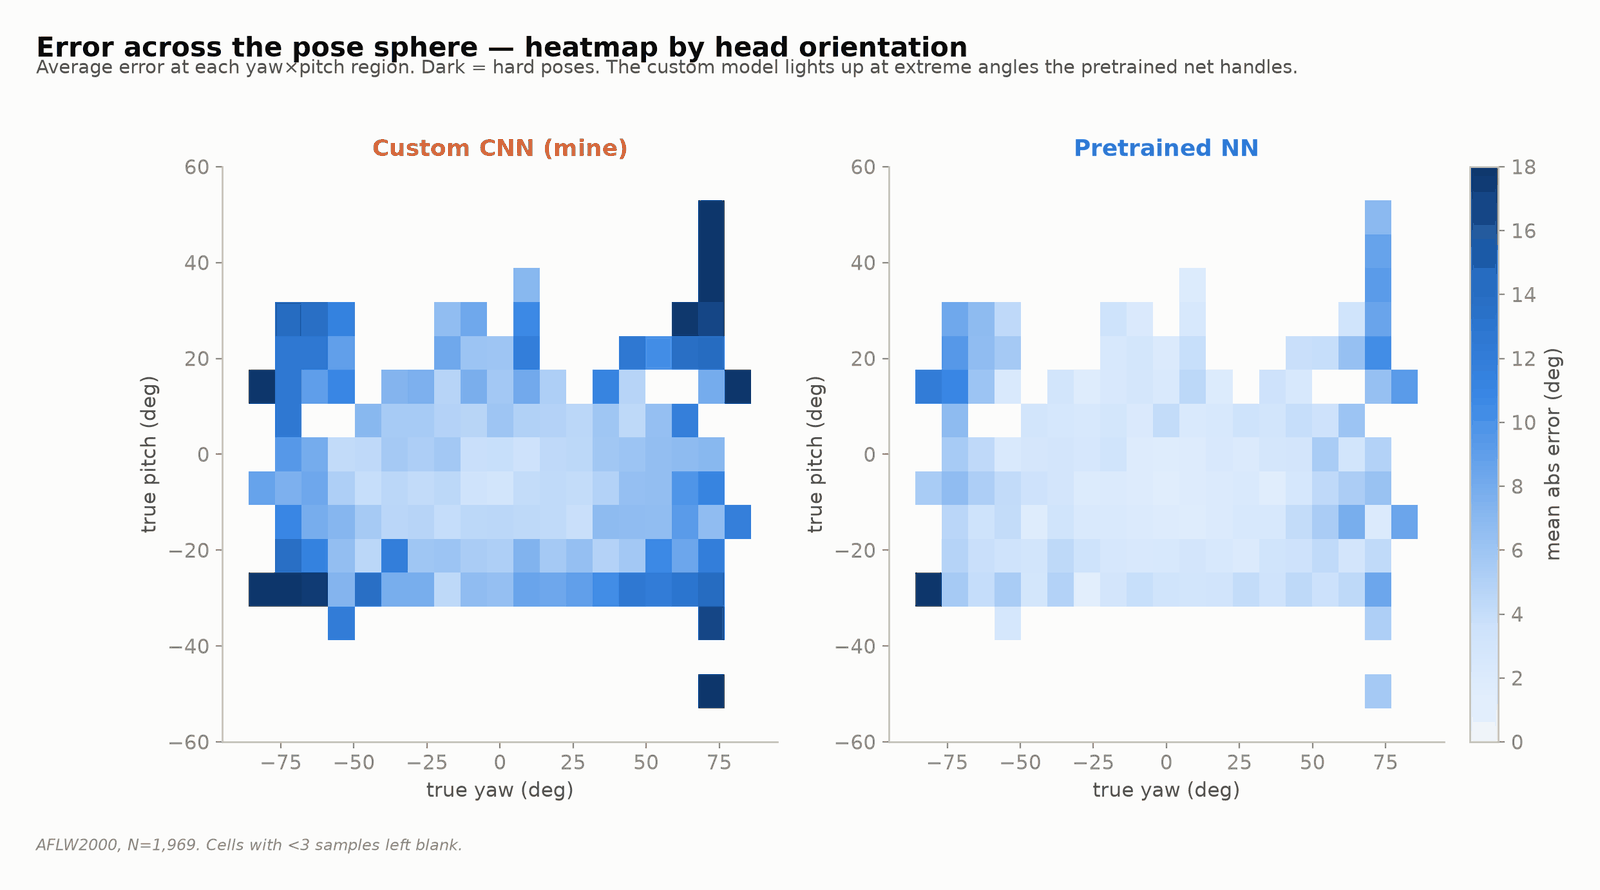
\includegraphics[width=\linewidth]{figures/headpose_H3_pose_heatmap.png}
\caption{Pose-sphere heat map --- mean error located in the yaw $\times$ pitch plane for each model.}
\label{fig:21}
\end{figure}

Three-axis mean error across four yaw bands is

\begin{equation}
\label{eq:235}
\begin{aligned}
A: 4.77^{\circ} (|\;\text{yaw}\;| < 15^{\circ}, n = 891)  \to \\
5.09^{\circ} (15\text{--}30^{\circ}, n = 420)  \to \\
8.08^{\circ} (30\text{--}60^{\circ}, n = 380)  \to \\
18.16^{\circ} (> 60^{\circ}, n = 278) ,
\end{aligned}
\end{equation}

\begin{equation}
\label{eq:236}
R: 2.35^{\circ} \to 2.47^{\circ} \to 3.81^{\circ} \to 8.20^{\circ} ,
\end{equation}

a 3.8$\times$ degradation for the proposed network against 3.5$\times$ for the baseline. The proposed-to-baseline ratio moves only from

\begin{equation}
\label{eq:237}
4.77/2.35 = 2.03 to 18.16/8.20 = 2.21
\end{equation}

across the entire manifold. Near-parallel degradation at a near-constant ratio is strong evidence against a localised failure mode: it is the manifold-level expression of \EQREF{211}, an approximately constant multiplicative loss of angular resolution everywhere. Critically for the interface, the region where error is largest --- beyond 60$^{\circ}$ --- lies well past the 30$^{\circ}$ trigger, so gesture reliability is governed by the two innermost bands, where error is 4.77$^{\circ}$ and 5.09$^{\circ}$ against an 18$^{\circ}$ hysteresis band. Expressing this as a margin,

\begin{equation}
\label{eq:238}
\mathrm{margin} = ( \theta _{\mathrm{on}} - \theta _{\mathrm{off}} ) / ( 2 \cdot e_{\mathrm{band}} ) = 18^{\circ} / ( 2 \times 5.09^{\circ} ) = 1.77 ,
\end{equation}

so a typical error must be nearly doubled before it can carry a pose across the band.

\FIGREF{22} gives the per-face view.

\begin{figure}[pos=htbp]
\centering
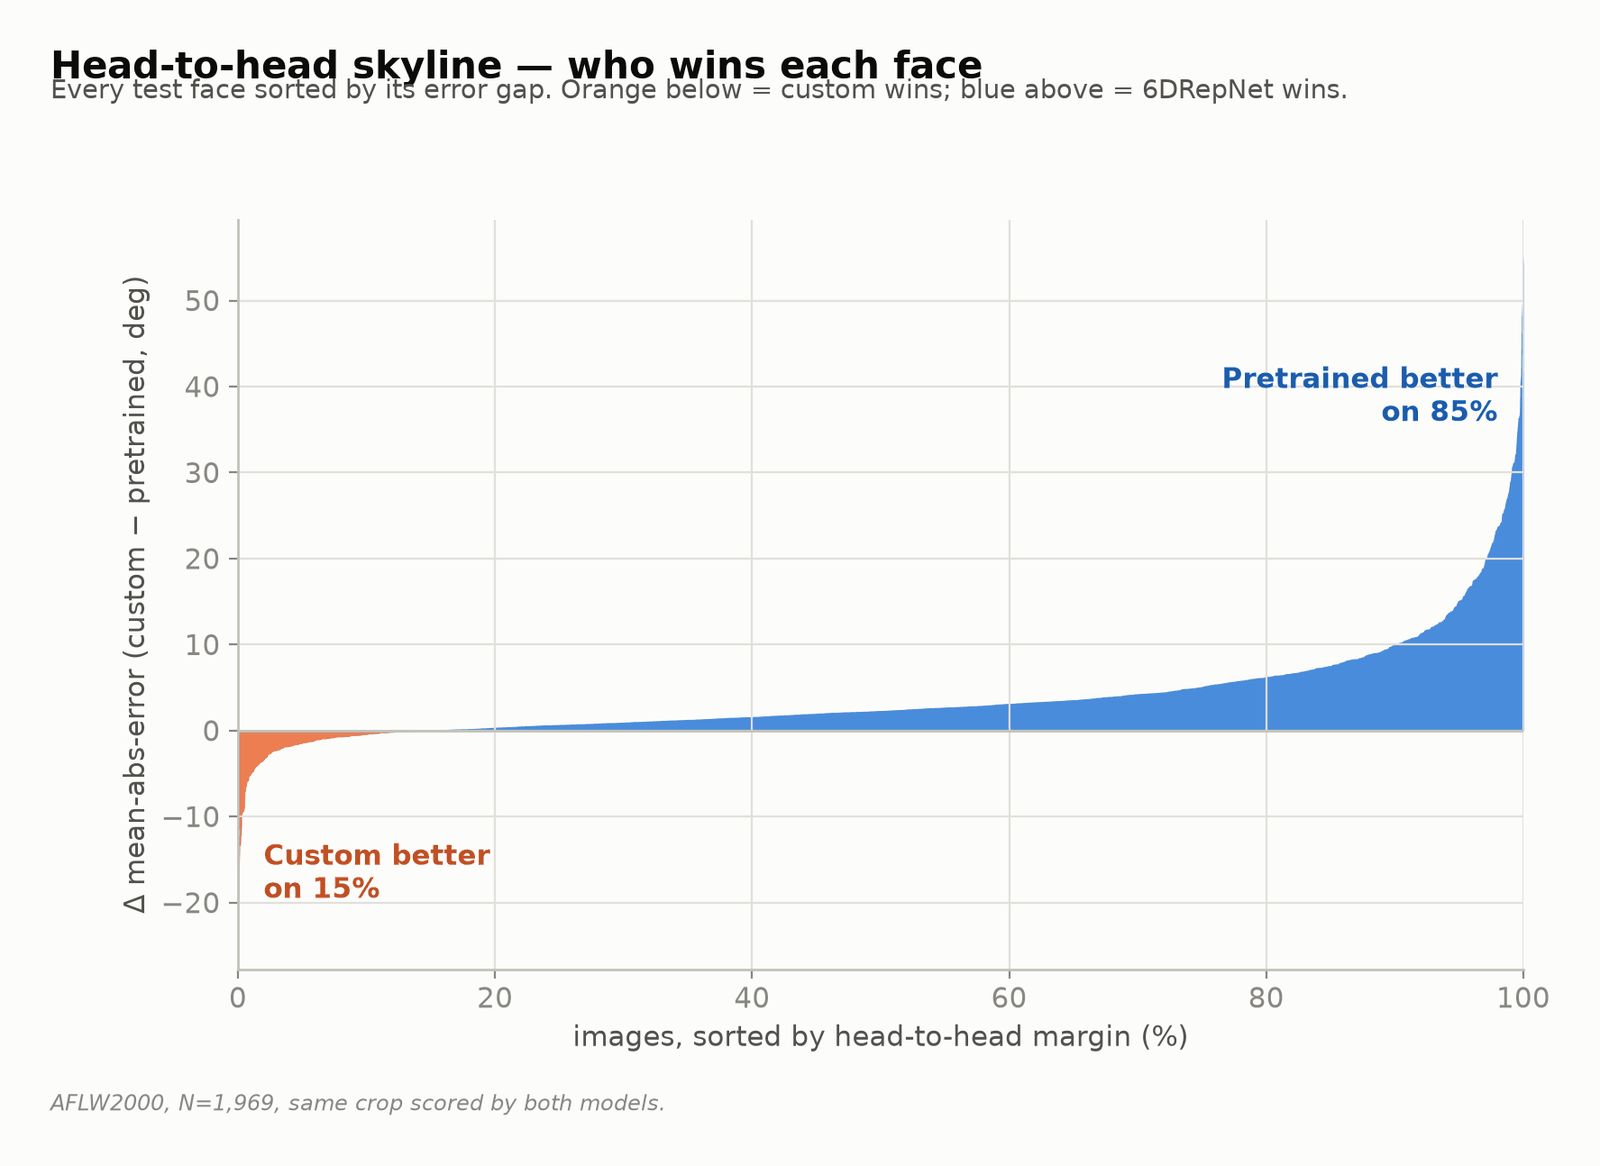
\includegraphics[width=\linewidth]{figures/headpose_H4_win_skyline.png}
\caption{Head-to-head skyline --- every AFLW2000 face sorted by its per-face error gap.}
\label{fig:22}
\end{figure}

Beyond the 14.58 \% win rate the extremes carry a caution. Catastrophic failures above 30$^{\circ}$ number 63 for the proposed network (3.20 \% of faces, contributing 1.36$^{\circ}$ of its 7.37$^{\circ}$ MAE) and 9 for the baseline (0.46 \%, 0.23$^{\circ}$ of 3.48$^{\circ}$). Their contribution to the aggregate is

\begin{equation}
\label{eq:239}
\begin{aligned}
\mathrm{contribution} = (1/n) \Sigma _{i \in \mathcal{C}} e(i) , \\
\mathcal{C} = { i : e(i) > 30^{\circ} } ,
\end{aligned}
\end{equation}

and excluding them leaves 6.01$^{\circ}$ against 3.25$^{\circ}$, so the gap is not outlier-driven. But the baseline's single worst error (119.6$^{\circ}$) \emph{exceeds} the proposed network's (92.6$^{\circ}$). The more accurate model owns the larger extreme, which argues against selecting architectures on maximum-error criteria over test sets of this size --- the maximum of n draws is an inconsistent statistic whose expectation grows with n for any heavy-tailed error law --- and which matters here because a single 90$^{\circ}$+ error inside a dwell window is exactly the event the 1,200 ms cooldown exists to contain.

\FIGREF{23} stratifies by yaw band, where the shrinkage account is directly testable.

\begin{figure}[pos=htbp]
\centering
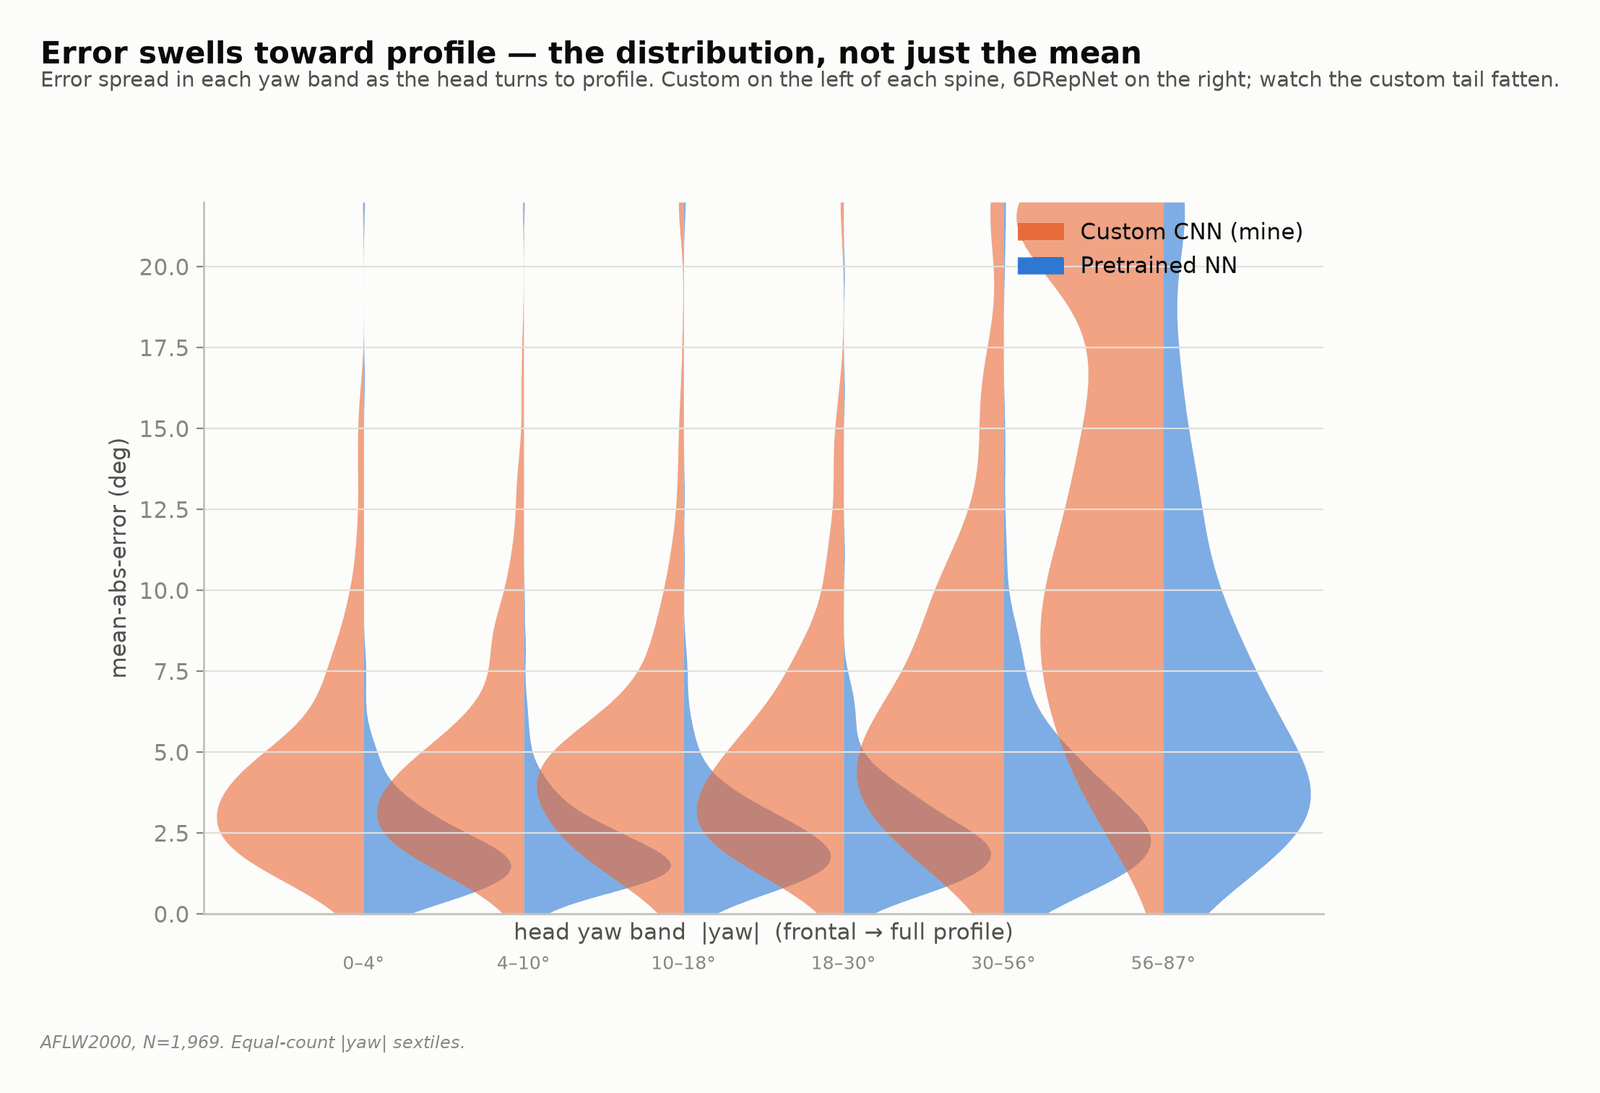
\includegraphics[width=\linewidth]{figures/headpose_H5_yaw_ridgeline.png}
\caption{Error versus profile --- error distributions per yaw band, from frontal through to full profile.}
\label{fig:23}
\end{figure}

Yaw-axis MAE runs 6.11$^{\circ}$, 6.98$^{\circ}$, 9.78$^{\circ}$ and 18.43$^{\circ}$ across the four bands, while the error predicted by gain deficiency alone,

\begin{equation}
\label{eq:240}
\hat{e}_{\mathrm{shrink}}(\text{band}) = ( 1 - \hat{s}_{\mathrm{yaw}} ) \cdot \mathbb{E}[ |\theta _{\mathrm{yaw}}| | \;\text{band} ] = 0.178 \cdot \mathbb{E}[ |\theta _{\mathrm{yaw}}| | \;\text{band} ] ,
\end{equation}

runs 1.13$^{\circ}$, 3.89$^{\circ}$, 7.99$^{\circ}$ and 12.64$^{\circ}$. The explained fraction

\begin{equation}
\label{eq:241}
\hat{e}_{\mathrm{shrink}} / e_{\mathrm{observed}} : 18 \% \to 56 \% \to 82 \% \to 69 \%
\end{equation}

rises from 18 \% of observed error at frontal to a dominant share beyond 30$^{\circ}$. Shrinkage is thus a minor contributor near frontal and the dominant one at profile, accounting for the accelerating degradation without any additional failure mechanism. The distributions broaden and shift together rather than becoming bimodal; bimodality would indicate sign confusion from flip augmentation without the label inversion of \EQREF{26}, and its absence confirms the augmentation logic is correct.

The deployment consequence is precise and follows from \EQREF{130}:

\begin{equation}
\label{eq:242}
\theta _{\mathrm{true}}^{\mathrm{trigger}} = \theta _{\mathrm{on}} / \hat{s}_{\mathrm{yaw}} = 30^{\circ} / 0.822 = 36.5^{\circ} ,
\end{equation}

so a user must turn to roughly 36.5$^{\circ}$ of true yaw to cross a 30$^{\circ}$ trigger. This is a systematic, stable and learnable offset --- users adapt to it within a session --- rather than an erratic one, which is why the gesture layer remains usable at an 8.74$^{\circ}$ yaw MAE.

\FIGREF{24} gives the regression fits.

\begin{figure}[pos=htbp]
\centering
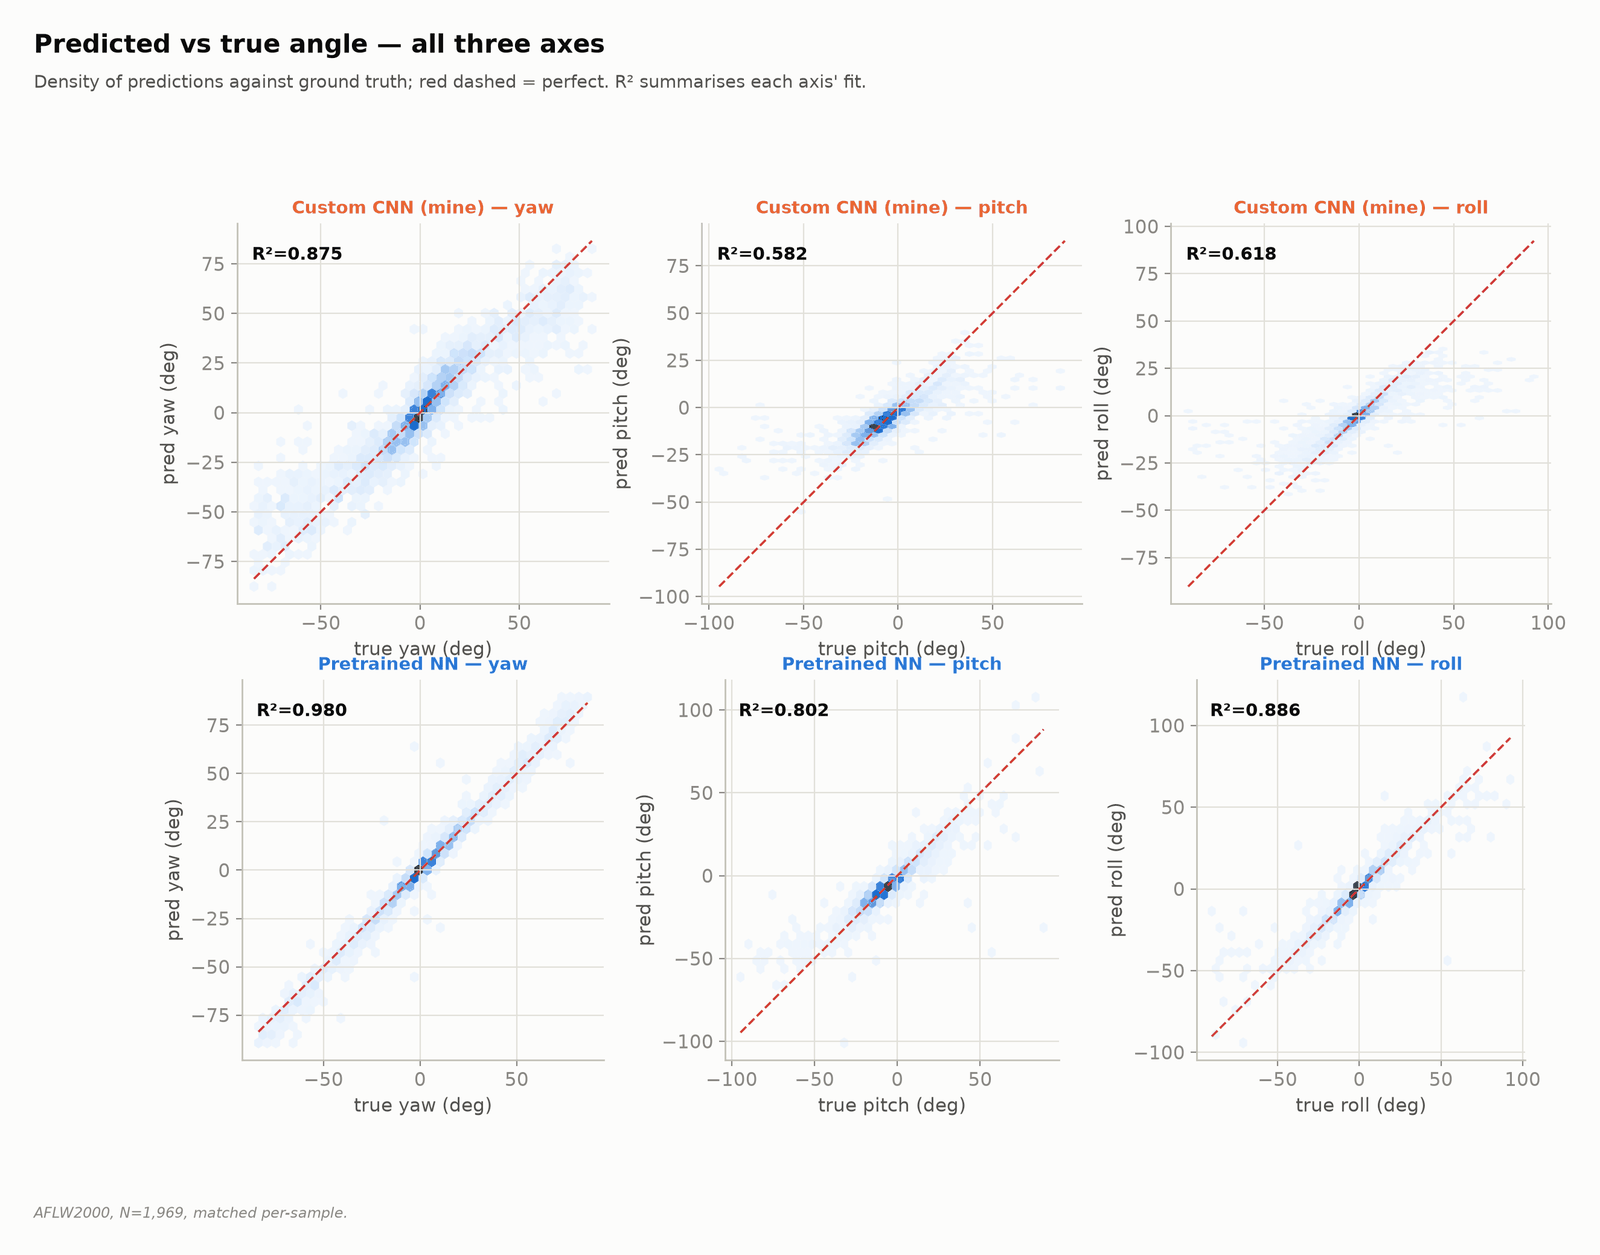
\includegraphics[width=\linewidth]{figures/headpose_H6_true_vs_pred.png}
\caption{Predicted versus true --- density-weighted fits with coefficient of determination for yaw, pitch and roll.}
\label{fig:24}
\end{figure}

Explained variance by \EQREF{153} is 87.5 \% for yaw, 61.8 \% for roll and 58.2 \% for pitch, against 98.0 \%, 88.6 \% and 80.2 \%. Read alongside the fitted slopes \EQREF{225} the two statistics separate cleanly: R$^{2}$ measures how much structure the network recovers, the slope whether it recovers it at the correct scale. Formally, by \EQREF{212} the two are related through

\begin{equation}
\label{eq:243}
R^{2} = \hat{s}^{2} \sigma _{\theta} ^{2} / ( \hat{s}^{2} \sigma _{\theta} ^{2} + \sigma _{\zeta} ^{2} ) ,
\end{equation}

so a high R$^{2}$ with a low $\hat{s}$ is the signature of \emph{low residual variance at contracted scale} --- the profile of an under-confident rather than an uninformed estimator. The proposed network scores comparatively well on the first and poorly on the second, and that is the reason a fixed trigger threshold rather than a learned one remains adequate: an under-confident estimator's output is a deterministic rescaling of the truth, which a fixed threshold accommodates by \EQREF{242}.

\FIGREF{25} locates the winner in pose space.

\begin{figure}[pos=htbp]
\centering
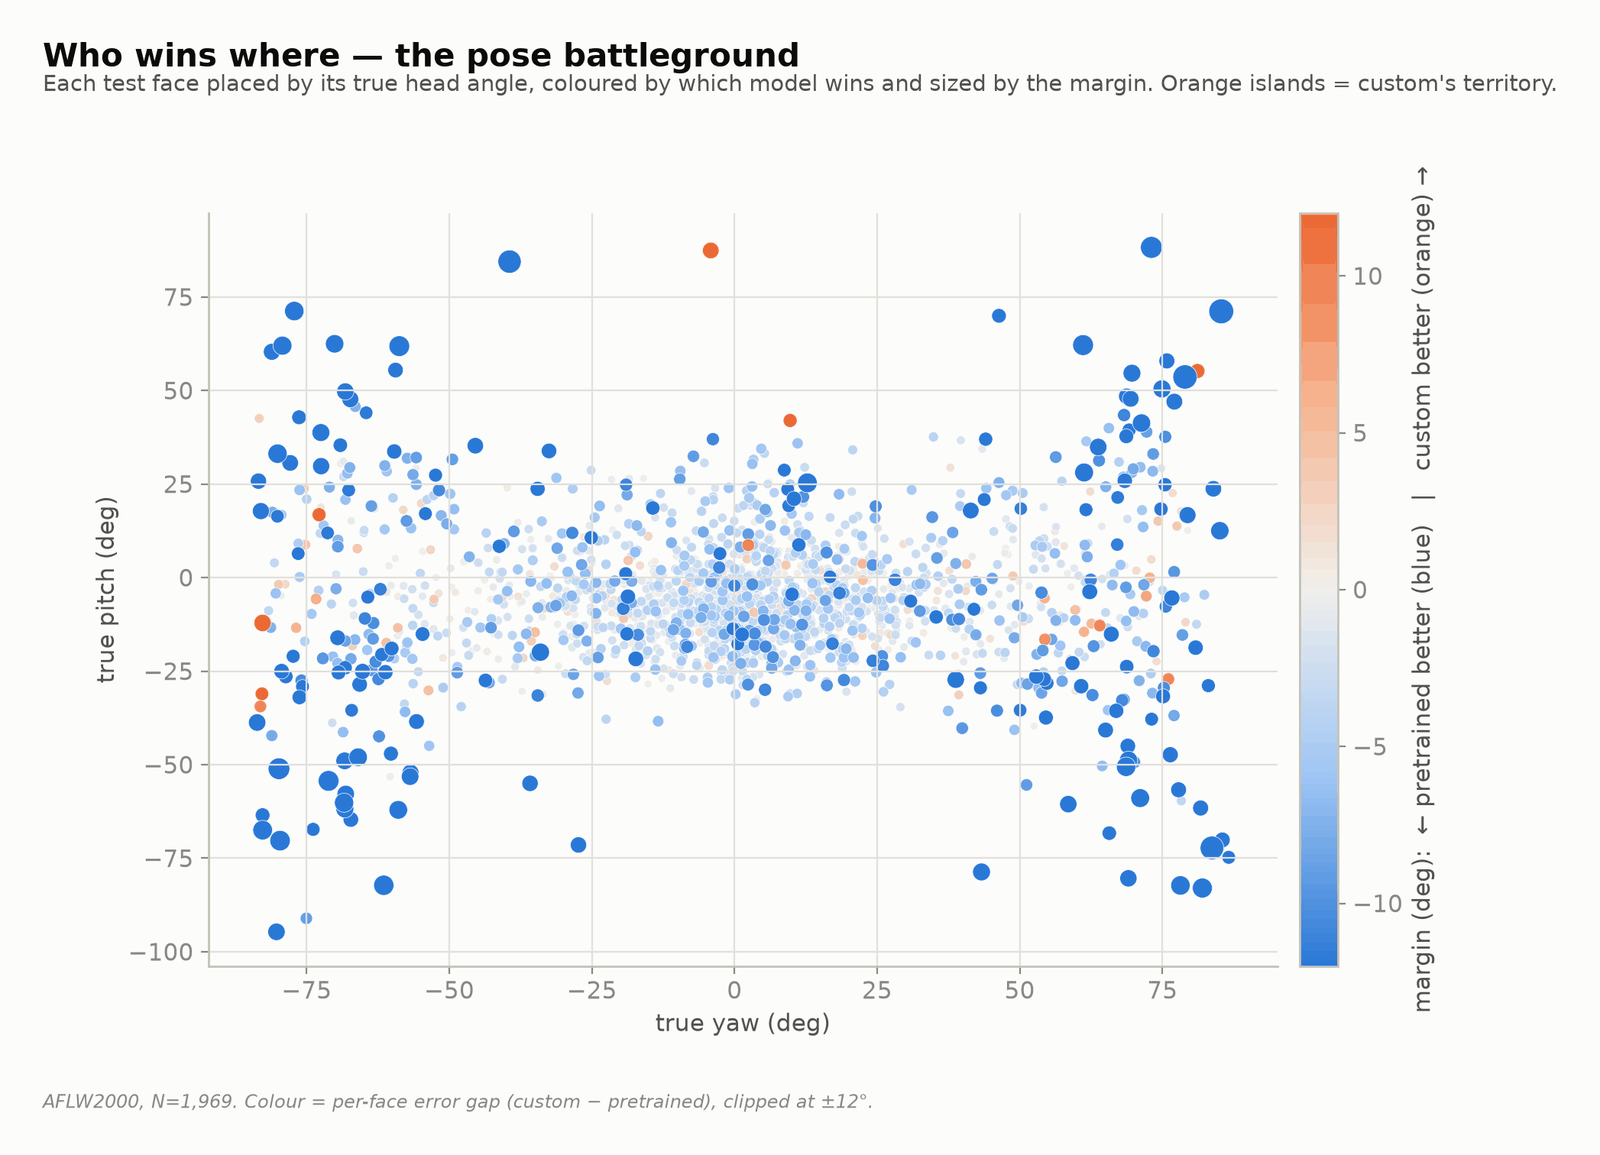
\includegraphics[width=\linewidth]{figures/headpose_H7_win_map.png}
\caption{Pose battleground --- every face placed at its true angle and coloured by which model achieves the lower error.}
\label{fig:25}
\end{figure}

Winning regions interleave rather than separating territorially, exactly as constant-ratio degradation predicts: with no pose region of systematic advantage, the wins are per-sample noise inside a dominated comparison. A pose-conditioned switching policy --- superficially attractive as a route to baseline accuracy at reduced average cost --- has no support here, and the $r_{\mathrm{AR}}$ = 0.671 error correlation independently confirms it would have little to exploit, since by \EQREF{164} the achievable gain is bounded by 7.5 \% even with an oracle.

\FIGRANGE{26}{29} re-render the same data as continuous fields, testing the joint claims of constant ratio, zero bias and benchmark sparsity.

\begin{figure}[pos=htbp]
\centering
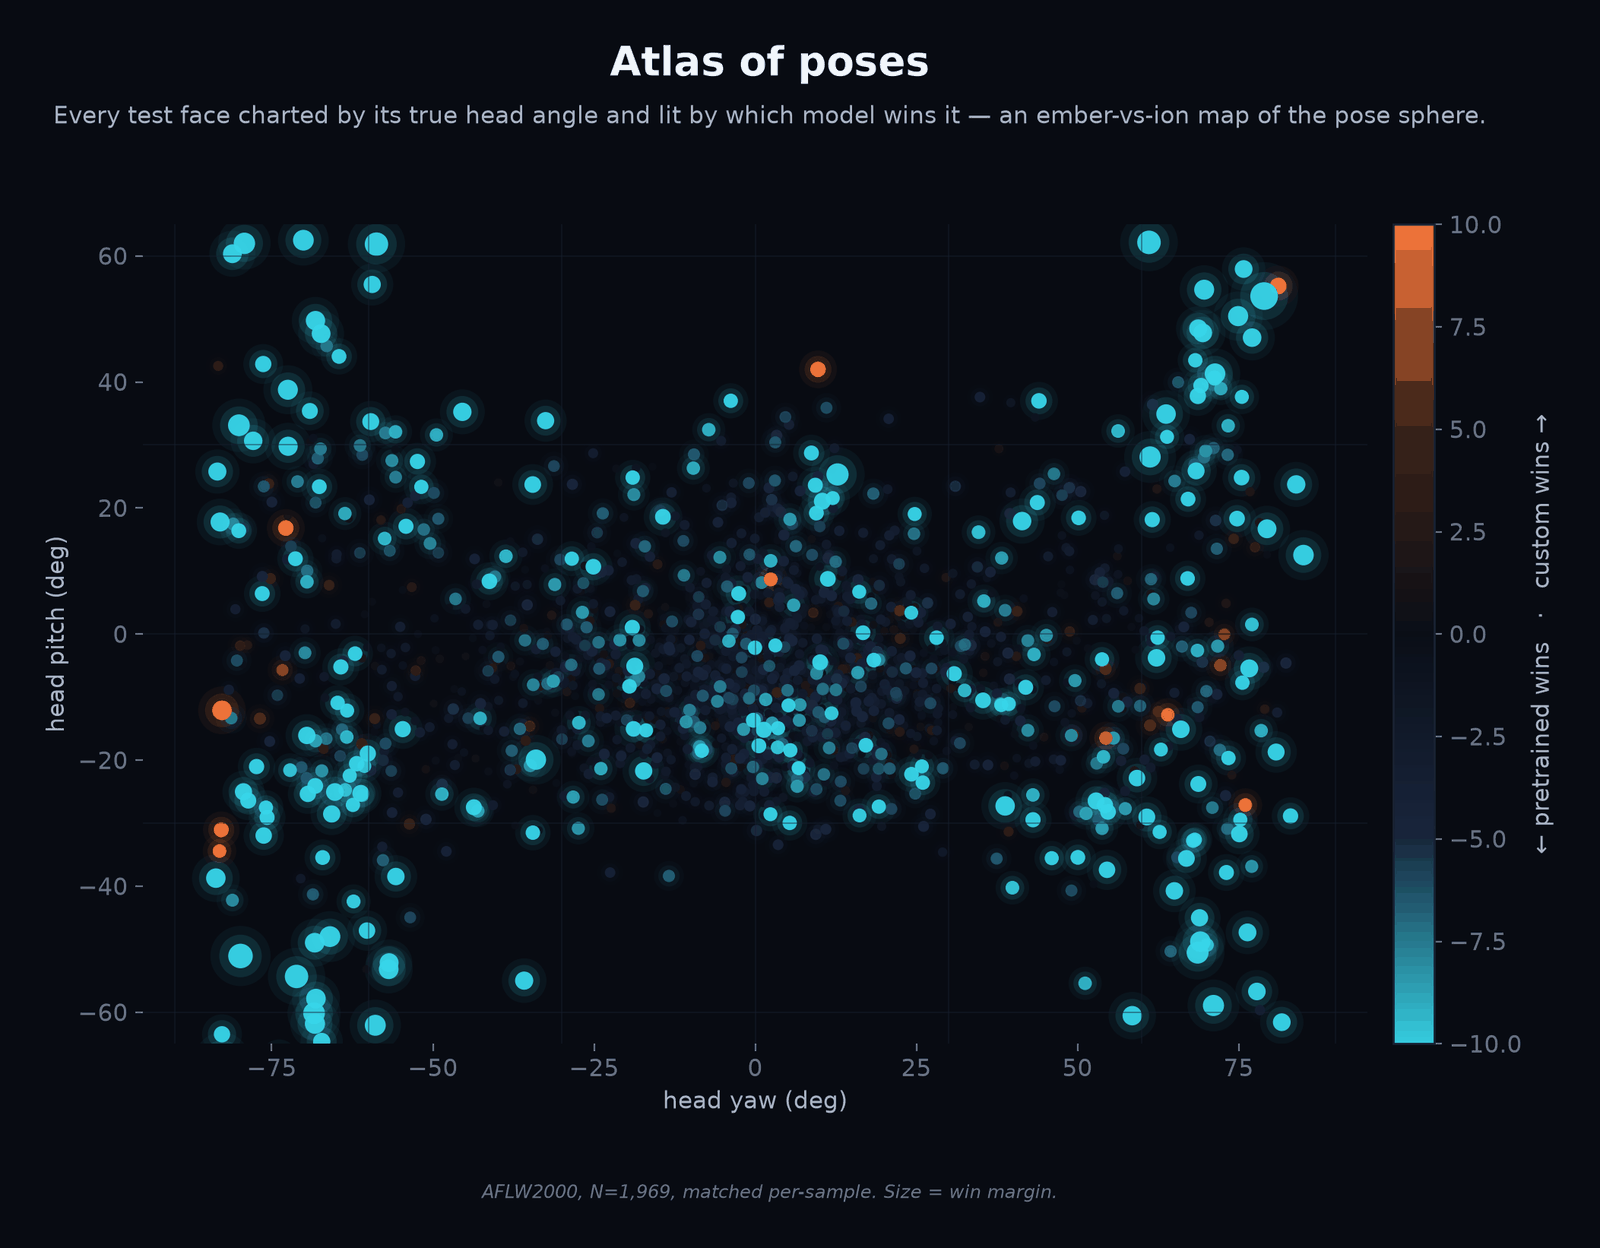
\includegraphics[width=\linewidth]{figures/figures_art_headpose_HA1_atlas.png}
\caption{Atlas of poses --- every AFLW2000 face charted at its true head angle and lit according to which model achieves the lower error.}
\label{fig:26}
\end{figure}

The continuous counterpart of \FIGREF{25} makes the absence of territory explicit: the 14.58 \% of faces won scatter with no contiguous region of advantage. Under a 2.03--2.21$\times$ ratio across the manifold by \EQREF{237}, scattered wins are what per-sample noise in a dominated comparison produces, and the $r_{\mathrm{AR}}$ = 0.671 correlation confirms the two models fail on the same faces. Two independent measurements --- one spatial, one rank-based --- converge on the same conclusion about fusion.

\begin{figure}[pos=htbp]
\centering
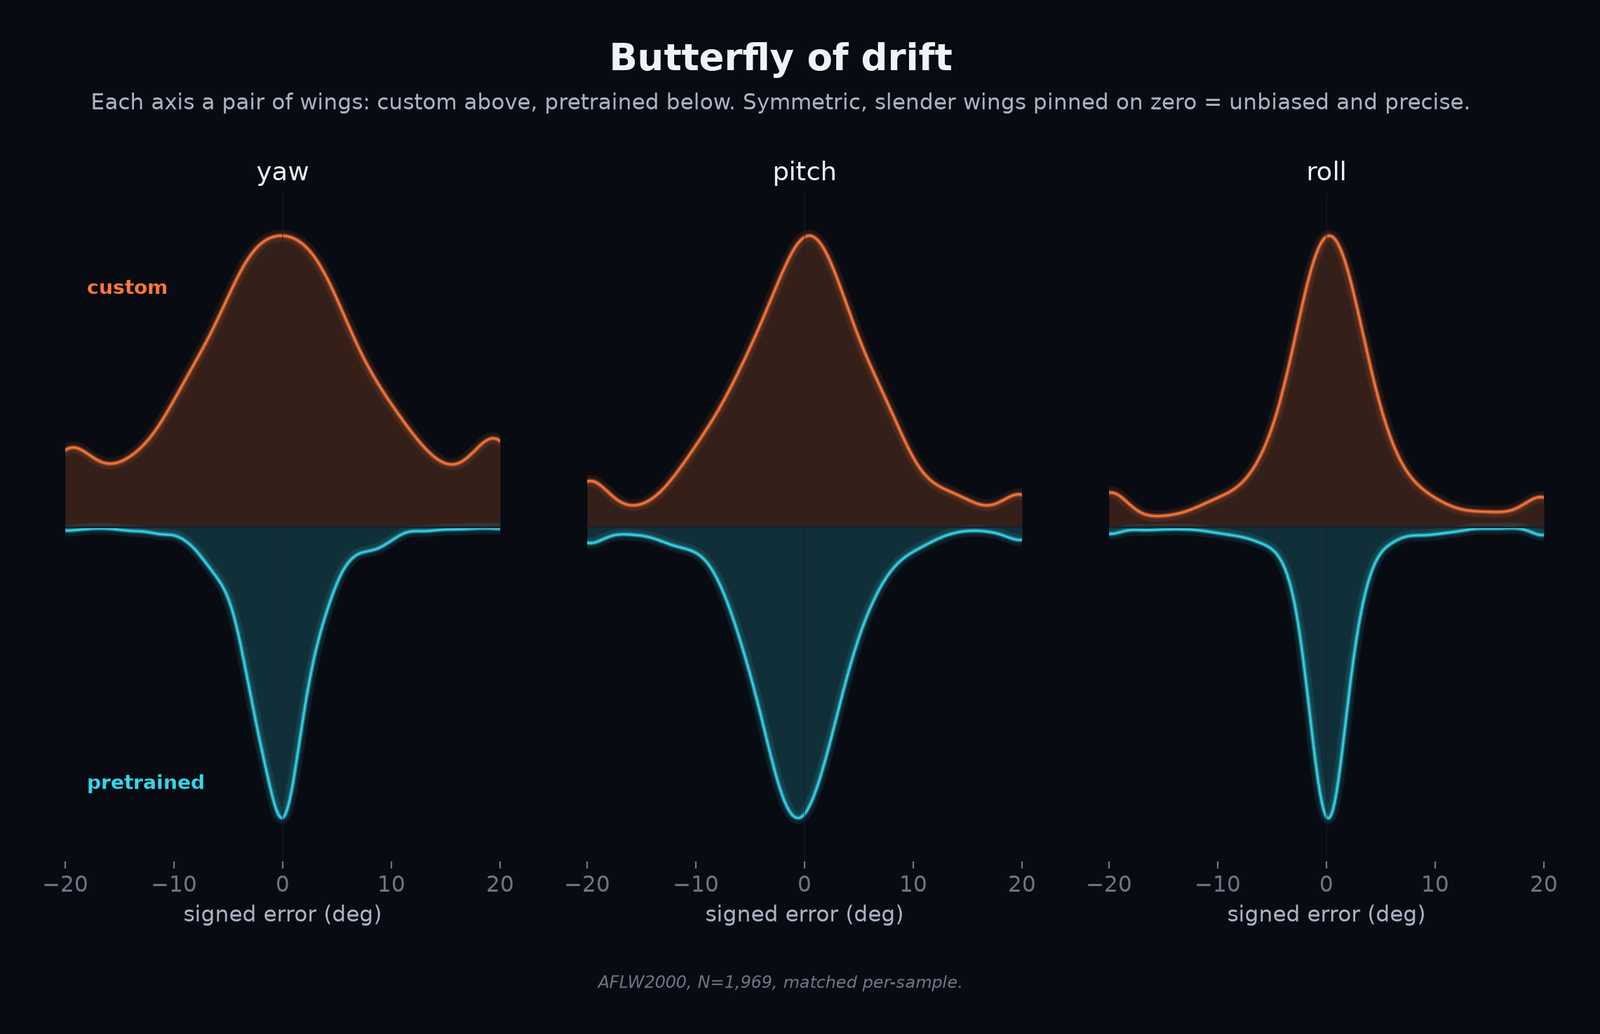
\includegraphics[width=\linewidth]{figures/figures_art_headpose_HA2_butterfly.png}
\caption{Butterfly of drift --- per-axis signed-error distributions, proposed network as the upper wing and the pretrained baseline as the lower wing of each pair.}
\label{fig:27}
\end{figure}

Every wing is pinned on zero by \EQREF{229}, so the deficit is width, not displacement. Spread ratios are

\begin{equation}
\label{eq:244}
\begin{aligned}
\sigma ^A/\sigma ^R: 2.49\times (\text{yaw}) , 1.46\times (\text{pitch}) , \\
1.84\times (\text{roll}) .
\end{aligned}
\end{equation}

That the yaw ratio is largest while yaw is also the best-explained (R$^{2}$ = 0.875) and least contracted ($\hat{s}$ = 0.822) axis is the visual statement of the units artefact of \EQREF{234} --- a modest relative deficit over a wide range produces the widest absolute distribution. The pinning on zero is what licenses the dwell-averaging argument of \EQREF{230}--\EQREF{231}.

\begin{figure}[pos=htbp]
\centering
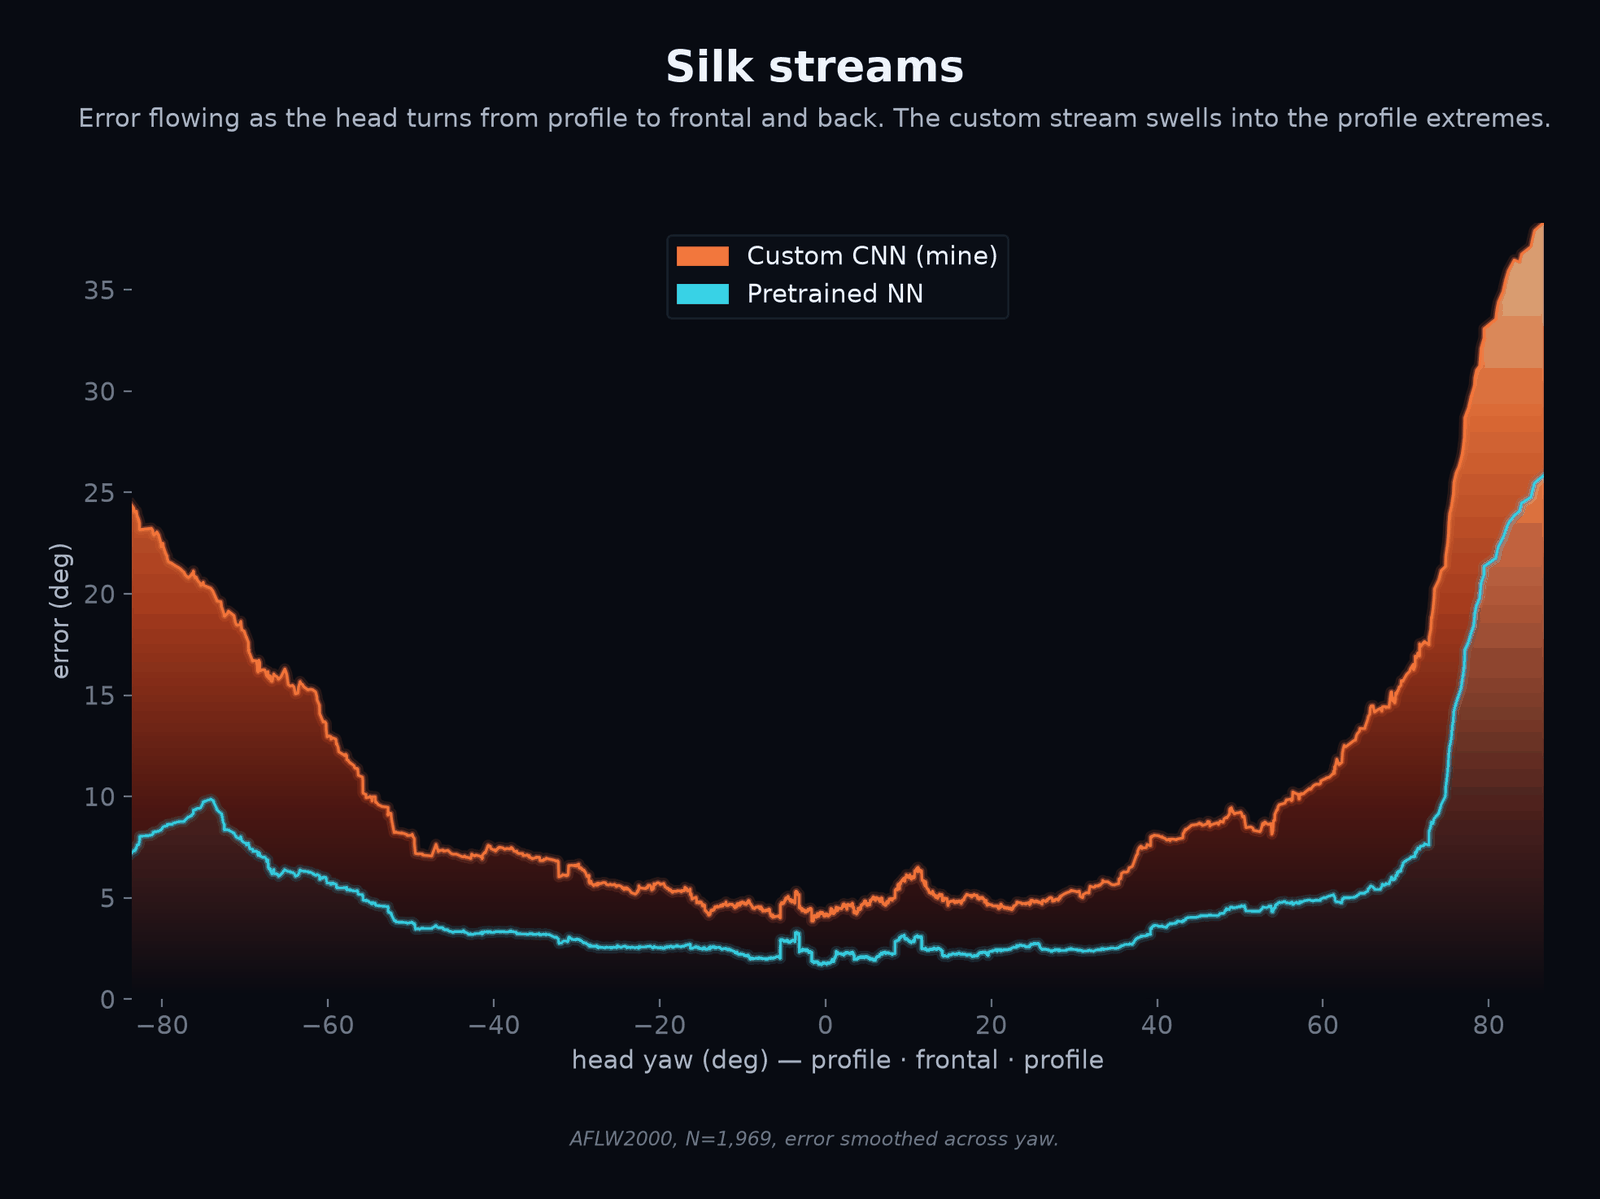
\includegraphics[width=\linewidth]{figures/figures_art_headpose_HA3_silk.png}
\caption{Silk streams --- error flowing as a continuous function of head rotation, from full profile through frontal and back.}
\label{fig:28}
\end{figure}

Continuity is the finding: the stream swells smoothly from 4.77$^{\circ}$ at frontal to 18.16$^{\circ}$ beyond 60$^{\circ}$ with no discontinuity or bifurcation, so the progressively occluded operator identified in \FIGREF{31} below degrades gracefully rather than failing abruptly. A discontinuity would signal a regime change, a bifurcation sign confusion; neither appears. Graceful degradation is what permits the gesture layer to stay stable at large angles, because error grows predictably with a state the state machine already tracks.

\begin{figure}[pos=htbp]
\centering
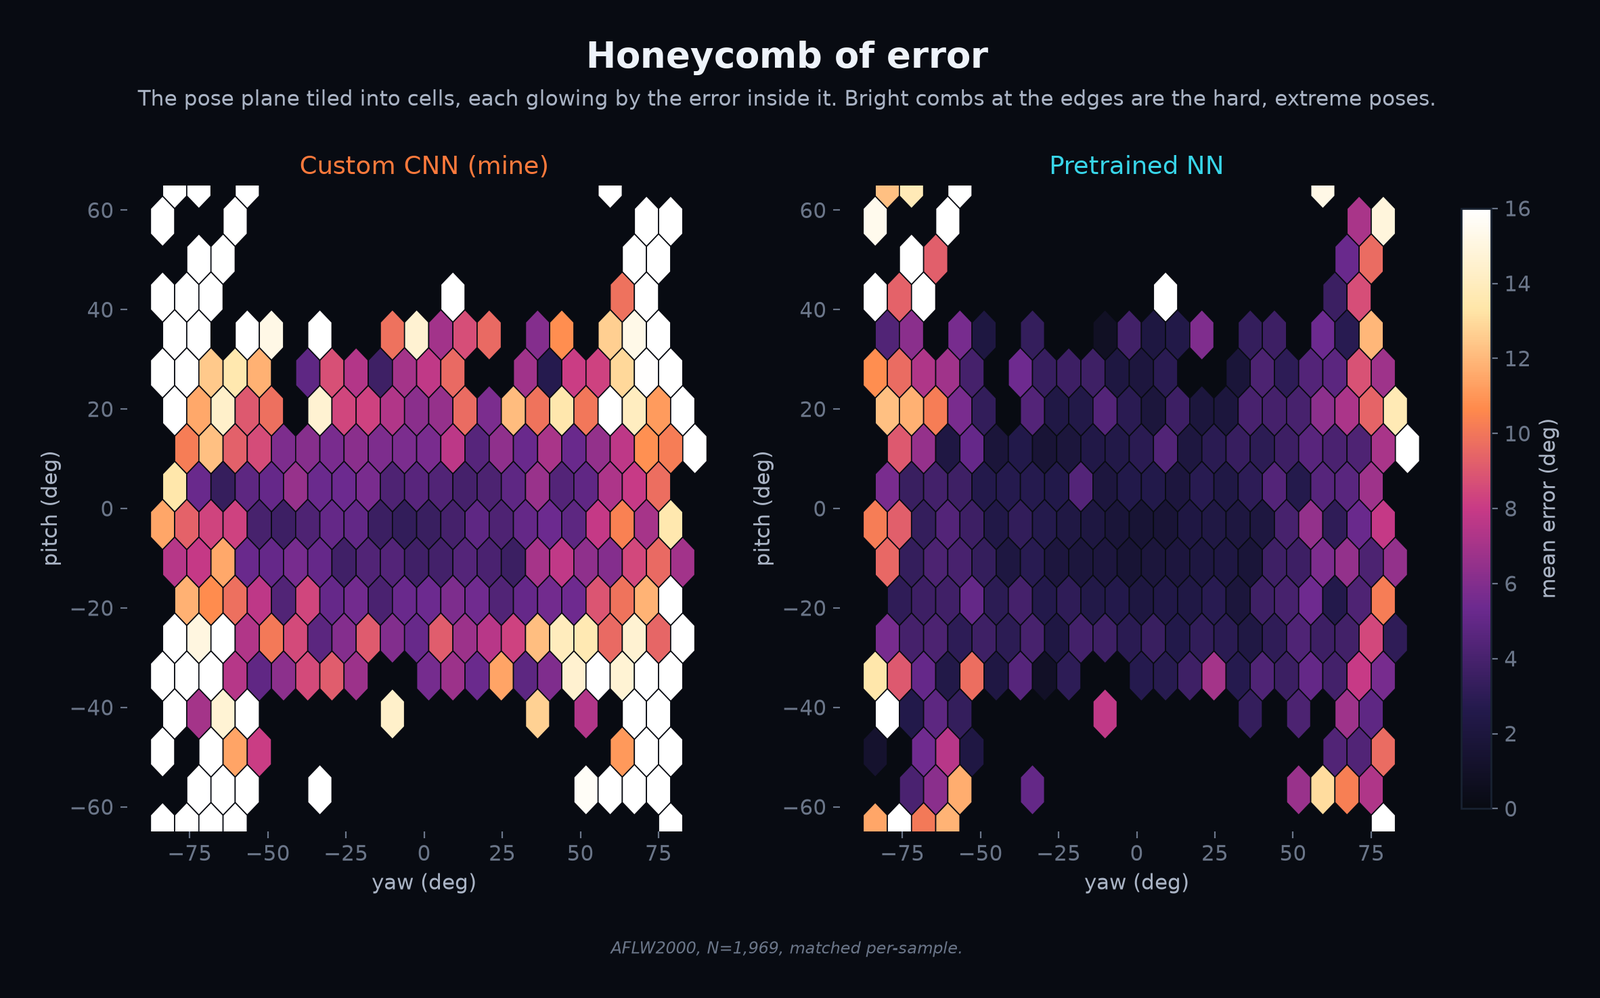
\includegraphics[width=\linewidth]{figures/figures_art_headpose_HA4_honeycomb.png}
\caption{Honeycomb of error --- the yaw $\times$ pitch plane tiled into cells, each glowing according to the mean error of the faces it contains.}
\label{fig:29}
\end{figure}

Tiling restores what smooth interpolation suppresses: cell occupancy. The brightest peripheral cells are the sparsest --- 278 of 1,969 faces lie beyond 60$^{\circ}$ of yaw against 891 within 15$^{\circ}$ --- so extreme-pose estimates rest on roughly a seventh of the evidence supporting frontal ones. The standard error of a band mean scales as

\begin{equation}
\label{eq:245}
\begin{aligned}
SE(\text{band}) = \sigma _{\mathrm{band}} / \sqrt{n}_{\mathrm{band}} , \\
SE(>60^{\circ})/SE(<15^{\circ}) = ( \sigma _{>60}/\sigma _{<15} ) \cdot \sqrt{891/278} \approx 1.79 \cdot ( \sigma \;\text{ratio} ) ,
\end{aligned}
\end{equation}

so the region where the models differ most is the region the benchmark constrains least, and the 18.16$^{\circ}$ against 8.20$^{\circ}$ comparison there carries materially wider uncertainty than its frontal counterpart. This caveat applies to AFLW2000-based comparisons generally, and it is reassuring for this system only because the operative range lies inside the well-populated bands.

\subsubsection{What the network computes}

\begin{figure}[pos=htbp]
\centering
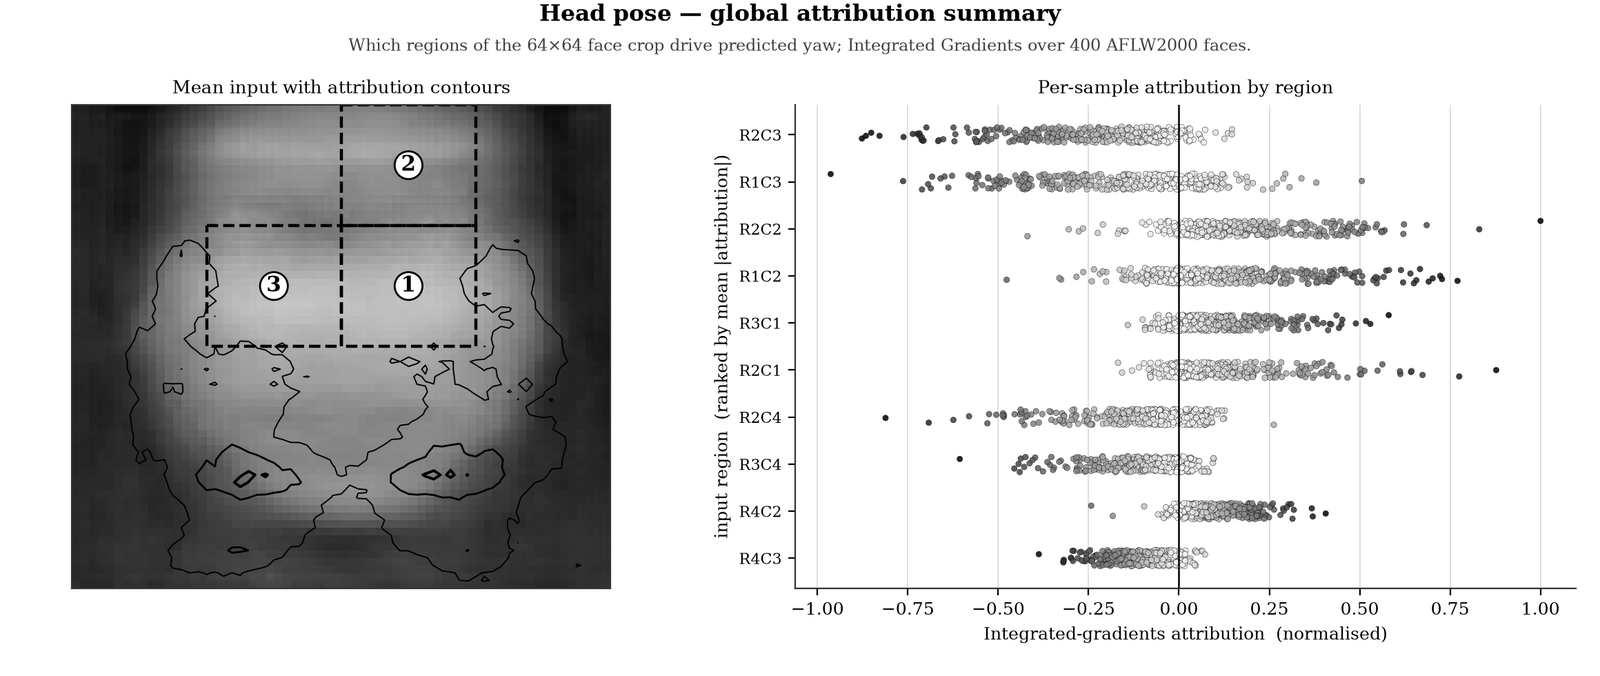
\includegraphics[width=\linewidth]{figures/attribution_headpose_A1_summary.png}
\caption{Head pose --- global attribution summary for predicted yaw over the 64 $\times$ 64 face crop.}
\label{fig:30}
\end{figure}

The attribution field is antisymmetric about the facial midline: columns 1--2 predominantly positive (R2C2, R1C2, R3C1, R2C1), columns 3--4 predominantly negative (R2C3, R1C3, R2C4, R3C4), with mass in the brow--eye--nose band of rows 1--3. Formally, writing the region attribution vector as a function of the mirror operator $\mathcal{M}$,

\begin{equation}
\label{eq:246}
\mathrm{Attr}( \mathcal{M} R_k ; x ) \approx - \mathrm{Attr}( R_k ; x ) \;\text{for k in the brow}\;--\;\text{eye}\;--\;\text{nose band} ,
\end{equation}

which is precisely the antisymmetric operator \EQREF{216} already identified for gaze. Yaw is physically encoded by the left--right asymmetry of that band under projection, and the network recovered exactly that computation --- structurally the same class of operator the gaze network learned, which is why both exhibit the same shrinkage behaviour: a differential operator's output amplitude falls as one of its two arguments is occluded, and \EQREF{155} then contracts the estimate. Row 4, jaw and chin, contributes little, a sensible allocation given it is the region most degraded by self-occlusion at profile.

\begin{figure}[pos=htbp]
\centering
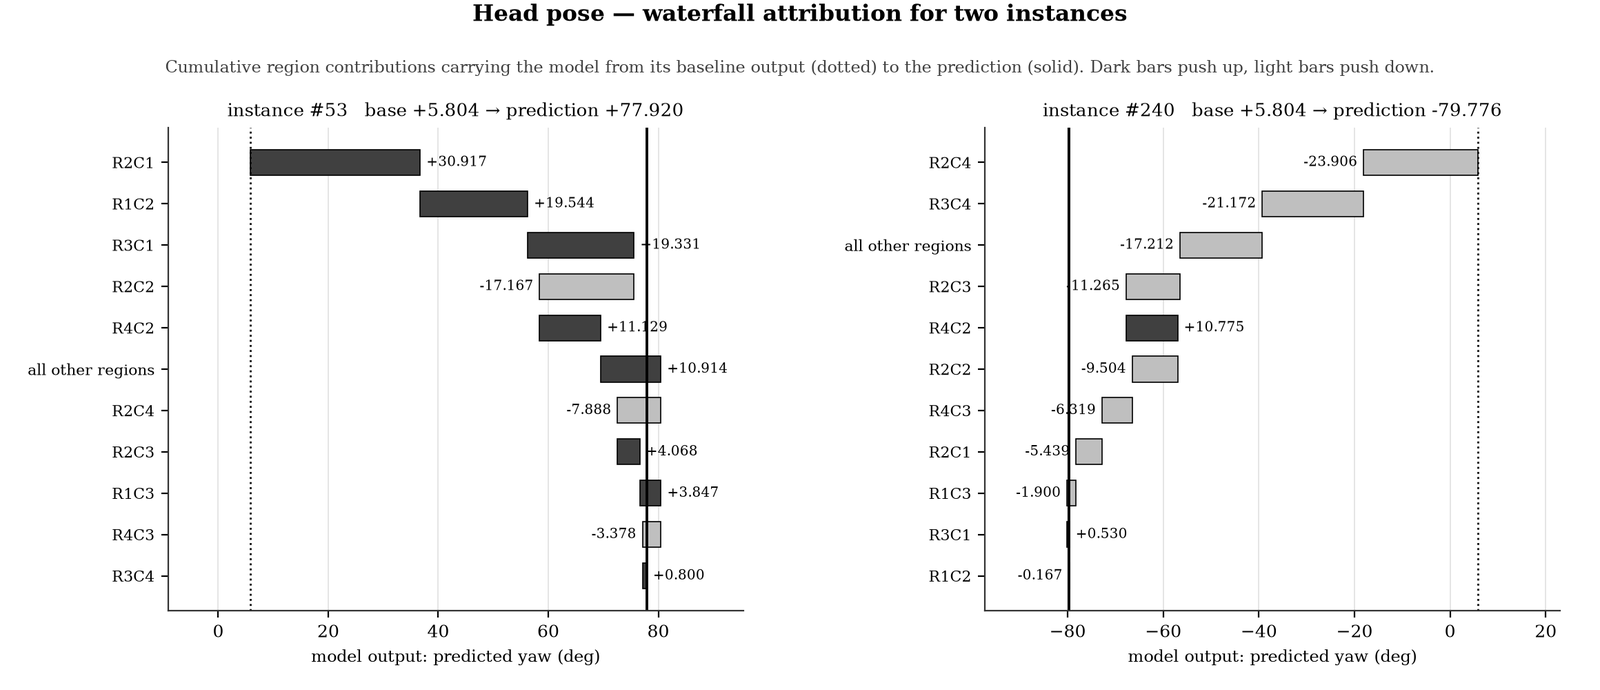
\includegraphics[width=\linewidth]{figures/attribution_headpose_A2_waterfall.png}
\caption{Head pose --- waterfall attribution for two extreme instances of predicted yaw.}
\label{fig:31}
\end{figure}

At extreme yaw the decomposition is dominated by one side of the antisymmetric pair, the occluded side contributing little. This is the mechanism generating the gain deficit of \FIGREF{23}. Modelling the differential operator's effective gain as a function of the visible fraction v($\theta_{\mathrm{yaw}}$) $\in$ [0,1] of the occluded hemiface,

\begin{equation}
\label{eq:247}
\begin{aligned}
s_{\mathrm{eff}}( \theta _{\mathrm{yaw}} ) = \sigma _{\theta} ^{2} / ( \sigma _{\theta} ^{2} + \sigma _{\varepsilon} ^{2}/v(\theta _{\mathrm{yaw}}) ) , \\
v \;\text{decreasing in}\; |\theta _{\mathrm{yaw}}| ,
\end{aligned}
\end{equation}

so that as yaw increases, half the differential measurement is lost to self-occlusion, effective gain falls, and the estimate compresses toward the frontal prior. Equation \EQREF{247} explains why contraction \emph{worsens with angle} rather than staying constant, matching the accelerating explained fraction of \EQREF{241}, and why no bimodality appears --- the operator degrades continuously rather than switching sign.

\begin{figure}[pos=htbp]
\centering
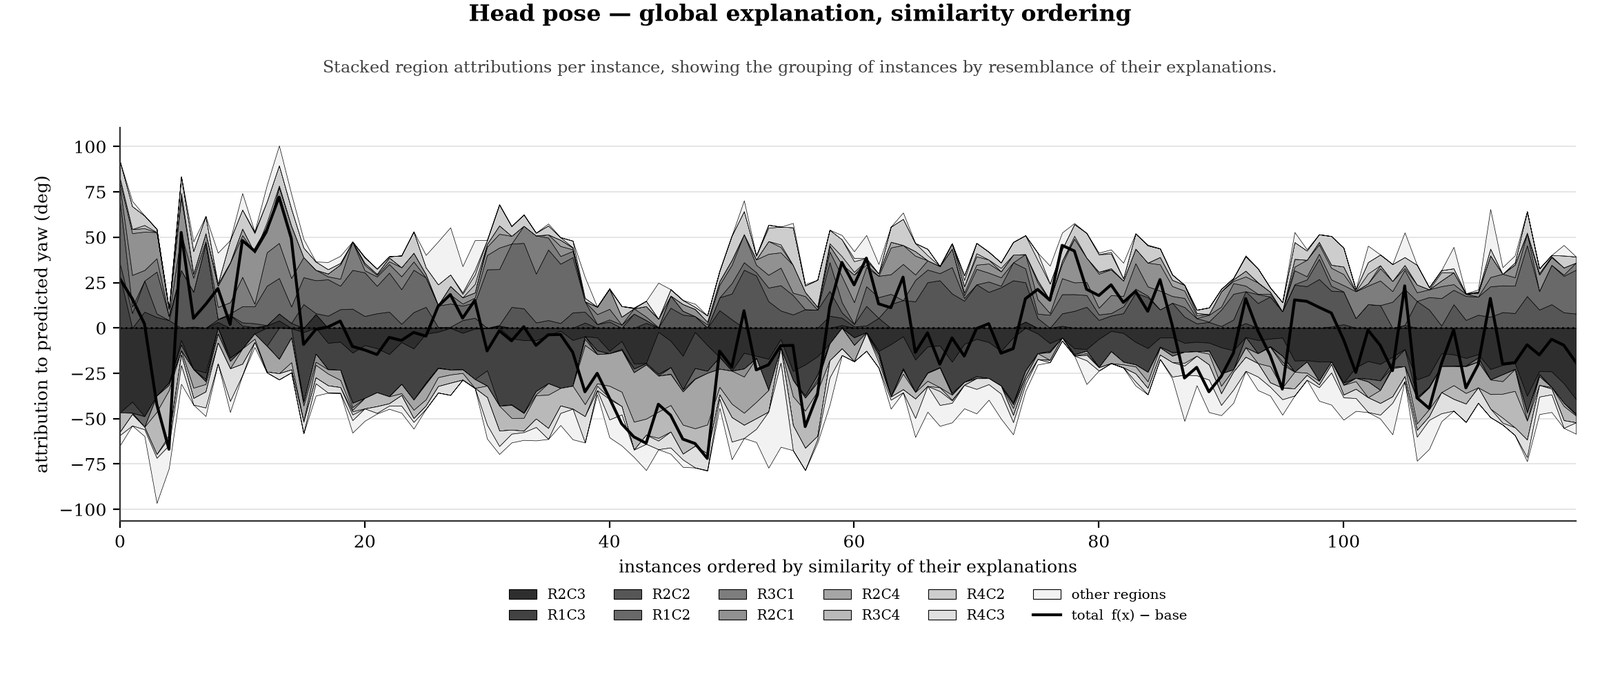
\includegraphics[width=\linewidth]{figures/attribution_headpose_A3_similarity.png}
\caption{Head pose --- global explanation under similarity ordering.}
\label{fig:32}
\end{figure}

Similarity ordering traces a smooth monotone progression of region weights following the pose manifold. No discontinuity appears anywhere along it, corroborating the constant-ratio degradation of \FIGREF{21} from an entirely independent measurement: there is no pose regime in which the network engages a qualitatively different strategy, only one in which the same strategy has less evidence available --- which is exactly the content of \EQREF{247}.

\begin{figure}[pos=htbp]
\centering
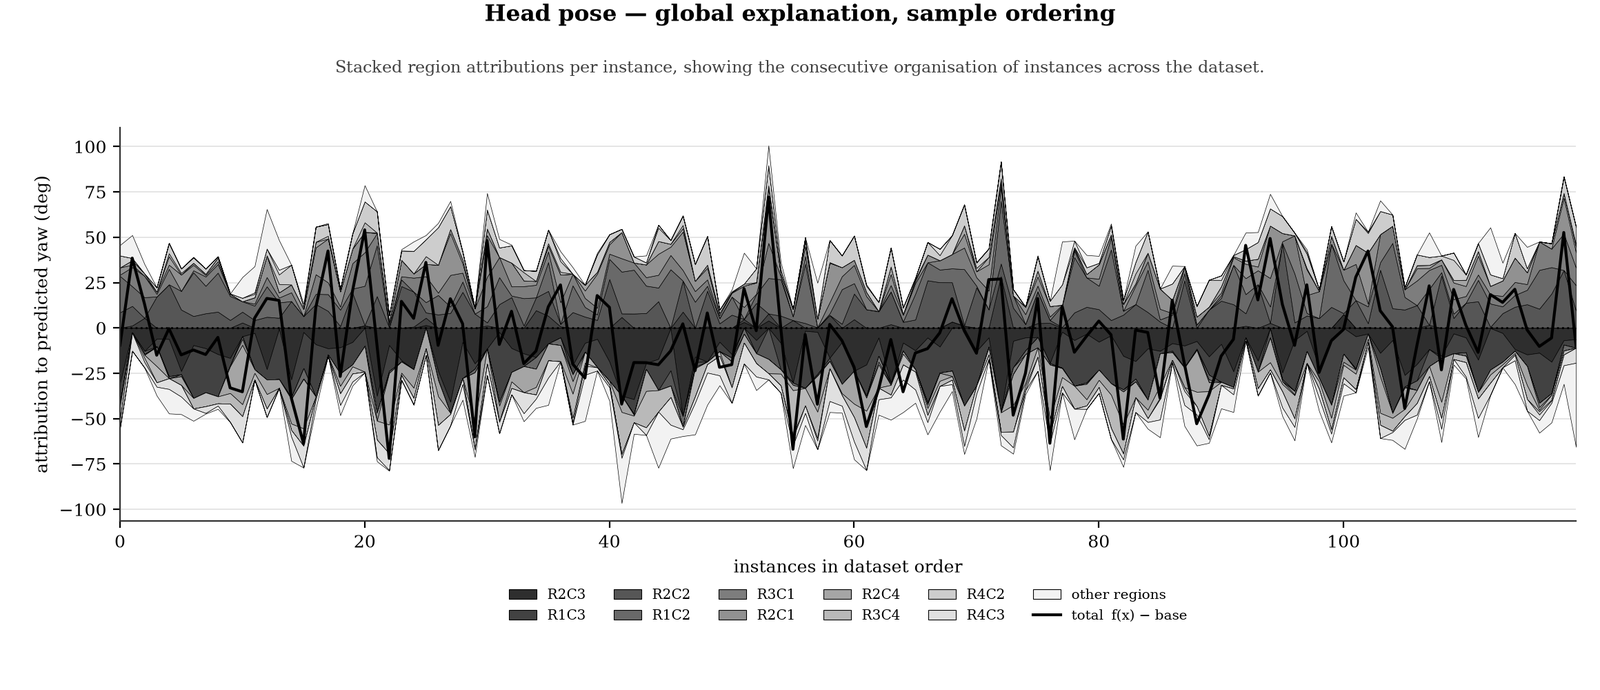
\includegraphics[width=\linewidth]{figures/attribution_headpose_A4_ordering.png}
\caption{Head pose --- global explanation under dataset ordering over AFLW2000.}
\label{fig:33}
\end{figure}

In dataset order the pattern is heterogeneous, reflecting AFLW2000's unordered pose composition. The absence of structure is the intended control: it confirms the coherent progression under similarity ordering in \FIGREF{32} is a property of the explanation manifold rather than an artefact of acquisition sequence, a distinction a single ordering could not have drawn.

\FloatBarrier

\subsection{Voice --- command execution}

Voice runs on its own audio thread, outside the camera loop's frame budget \EQREF{3}, and maps six keywords to the commands that make the rest of the interface operable: \emph{up} and \emph{down} scroll, \emph{stop} and \emph{go} pause and resume control, \emph{yes} and \emph{no} confirm and cancel. Its row in \TABREF{6} names per-class precision on the safety-critical words as the governing statistic, and the reason is consequence rather than frequency --- by \EQREF{135}, \emph{go} is the only route back once \emph{stop} has paused the system, so an error on it must be recovered by repetition against a system that is deliberately not acting. This section therefore reports per-class behaviour before aggregate behaviour, inverting the usual order.

On the 2,468-clip official test split the proposed network attains

\begin{equation}
\label{eq:248}
\begin{aligned}
\mathrm{Acc} = 94.53 \% , \mathrm{BalAcc} = 94.48 \% , \\
\;\text{macro}\;-F_{1} = 94.48 \% , \mathrm{MCC} = 0.9344 , \kappa = 0.9344 ,
\end{aligned}
\end{equation}

against the production ASR baseline at 95.50 \% accuracy and 97.43 \% macro-F$_{1}$. The 2.95 pp macro-F$_{1}$ gap is produced by a \emph{mechanism} rather than by discriminative superiority, and separating the two is the substance of this section.

\FIGREF{34} presents the error structure.

\begin{figure}[pos=htbp]
\centering
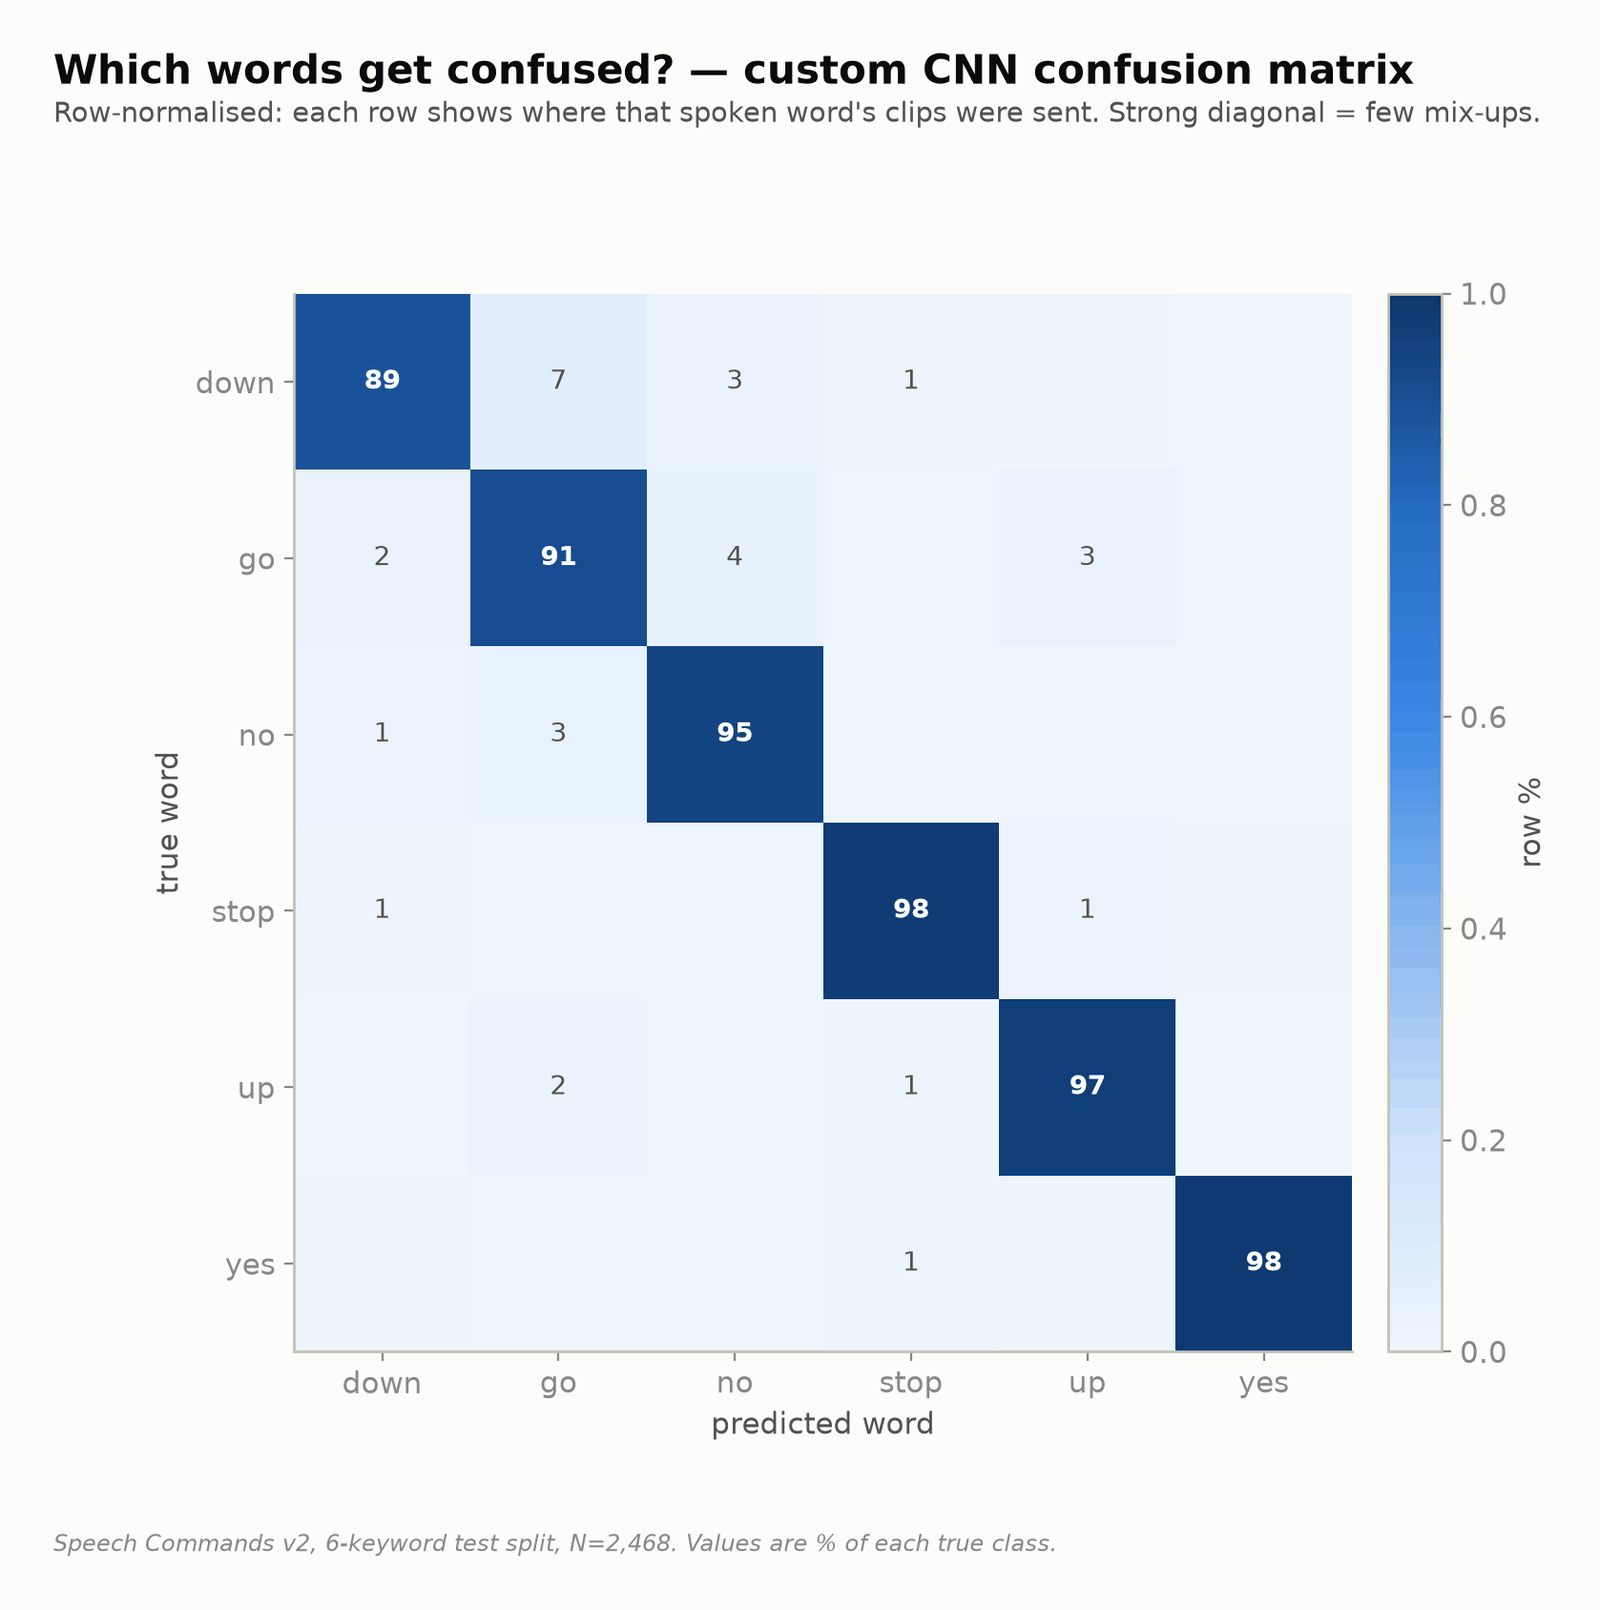
\includegraphics[width=\linewidth]{figures/voice_V1_confusion.png}
\caption{Confusion matrix --- row-normalised, showing where the clips of each spoken keyword were assigned.}
\label{fig:34}
\end{figure}

The 135 errors concentrate in three pairs: \emph{down} $\leftrightarrow$ \emph{go} (38 clips), \emph{go} $\leftrightarrow$ \emph{no} \EQREF{30} and \emph{down} $\leftrightarrow$ \emph{no} \EQREF{17}, together

\begin{equation}
\label{eq:249}
( 38 + 30 + 17 ) / 135 = 63.0 \%
\end{equation}

of all errors. All three involve a back rounded nucleus and differ principally in a brief initial consonant, so the discriminative evidence occupies a few tens of milliseconds at onset --- a small number of the T = 81 time frames produced by \EQREF{28}. The precision--recall split localises the mechanism:

\begin{equation}
\label{eq:250}
\begin{aligned}
\mathrm{Prec}(go) = 0.877 , \\
\mathrm{Rec}(go) = 0.908 ; \mathrm{Prec}(\text{down}) = 0.948 , \\
\mathrm{Rec}(\text{down}) = 0.889 .
\end{aligned}
\end{equation}

Since Prec(go) < Rec(go) while the reverse holds for \emph{down}, \emph{go} is an \textbf{attractor}: it absorbs clips from its phonetic neighbours rather than being a class the network fails to recognise. Formally, writing N(c'$\to$c) for the count of true-c' clips assigned to c, the in-flow/out-flow imbalance

\begin{equation}
\label{eq:251}
\Lambda _c = \Sigma _{c' \neq c} N_{c'\to c} - \Sigma _{c' \neq c} N_{c\to c'}
\end{equation}

is positive for \emph{go} and negative for \emph{down}, which is the quantitative content of ``attractor''.

For the interface this is the most consequential single result in the voice evaluation, and it is a \textbf{design fault rather than a model fault}. \emph{go} is bound to ``resume control'': the command that reactivates the interface after \emph{stop} has suspended it. Its being an attractor means spurious resumes while the system is deliberately paused; its 0.877 precision is the worst in the vocabulary; and its partners in confusion are \emph{down} (scroll) and \emph{no} (escape), both frequently spoken. Meanwhile \emph{stop}, the pause direction, is among the strongest words (precision 0.971, recall 0.976). The safety-critical asymmetry therefore runs the wrong way --- the gate is easy to close and easy to open accidentally --- and the remedy costs nothing: rebinding ``resume control'' to a phonetically distant token, one with fricative or stop-cluster onset (the acoustic class that \FIGREF{37} below shows the network separates best), removes the largest error mode without retraining a single parameter.

\FIGREF{35} places the proposed network against the ASR baseline across shared metrics.

\begin{figure}[pos=htbp]
\centering
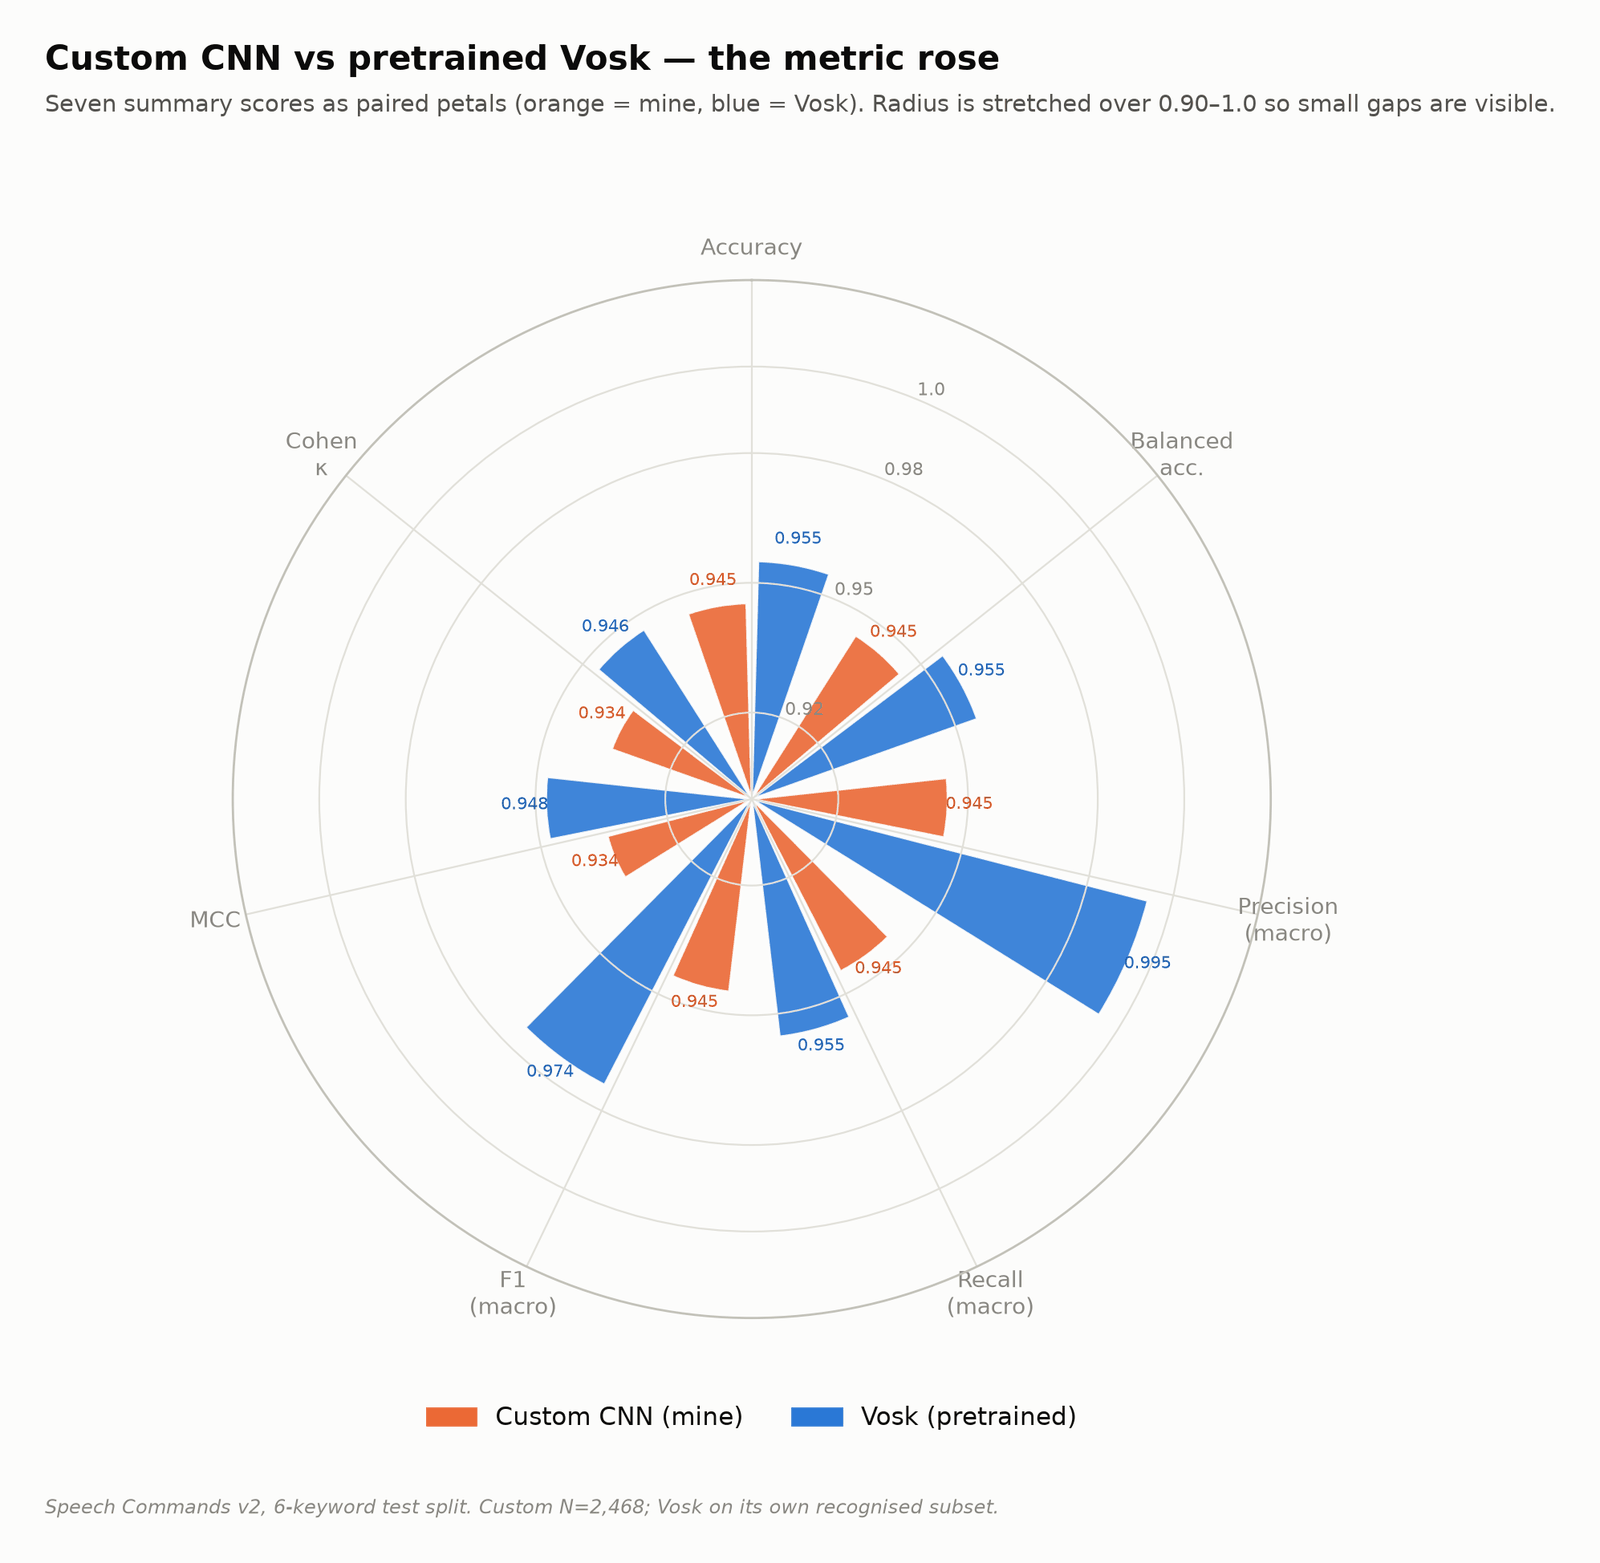
\includegraphics[width=\linewidth]{figures/voice_V2_metric_rose.png}
\caption{Metric rose --- seven summary scores as paired petals, proposed network against the pretrained ASR baseline.}
\label{fig:35}
\end{figure}

The baseline's macro precision is 99.45 \% against 94.53 \% while its macro recall is 95.53 \% against 94.48 \%, and the divergence is explained entirely by abstention. The engine rejects 98 of 2,468 clips, emitting no hypothesis, and among the 2,370 it does transcribe it commits only 13 substitutions:

\begin{equation}
\label{eq:252}
\mathrm{cov}_R = 2370/2468 = 96.03 \% , \mathrm{risk}_R = 13/2370 = 0.55 \% .
\end{equation}

It is not a more discriminative classifier but one equipped with a rejection option in the sense of \EQREF{132}, converting would-be substitutions into non-responses. Macro-F$_{1}$ rewards this --- abstention costs recall but protects precision --- whereas forced-choice accuracy, the like-for-like comparison under \EQREF{131}, differs by only

\begin{equation}
\label{eq:253}
95.50 \% - 94.53 \% = 0.97 pp .
\end{equation}

In this interface the distinction is operational rather than semantic: under the asymmetric loss \EQREF{134} a substitution executes an unintended command while an abstention costs one repetition, and given the \emph{go} binding above the abstention is clearly preferable.

\FIGREF{36} asks whether the same rejection regime is available to the proposed network, which requires its confidence to be a probability rather than a ranking.

\begin{figure}[pos=htbp]
\centering
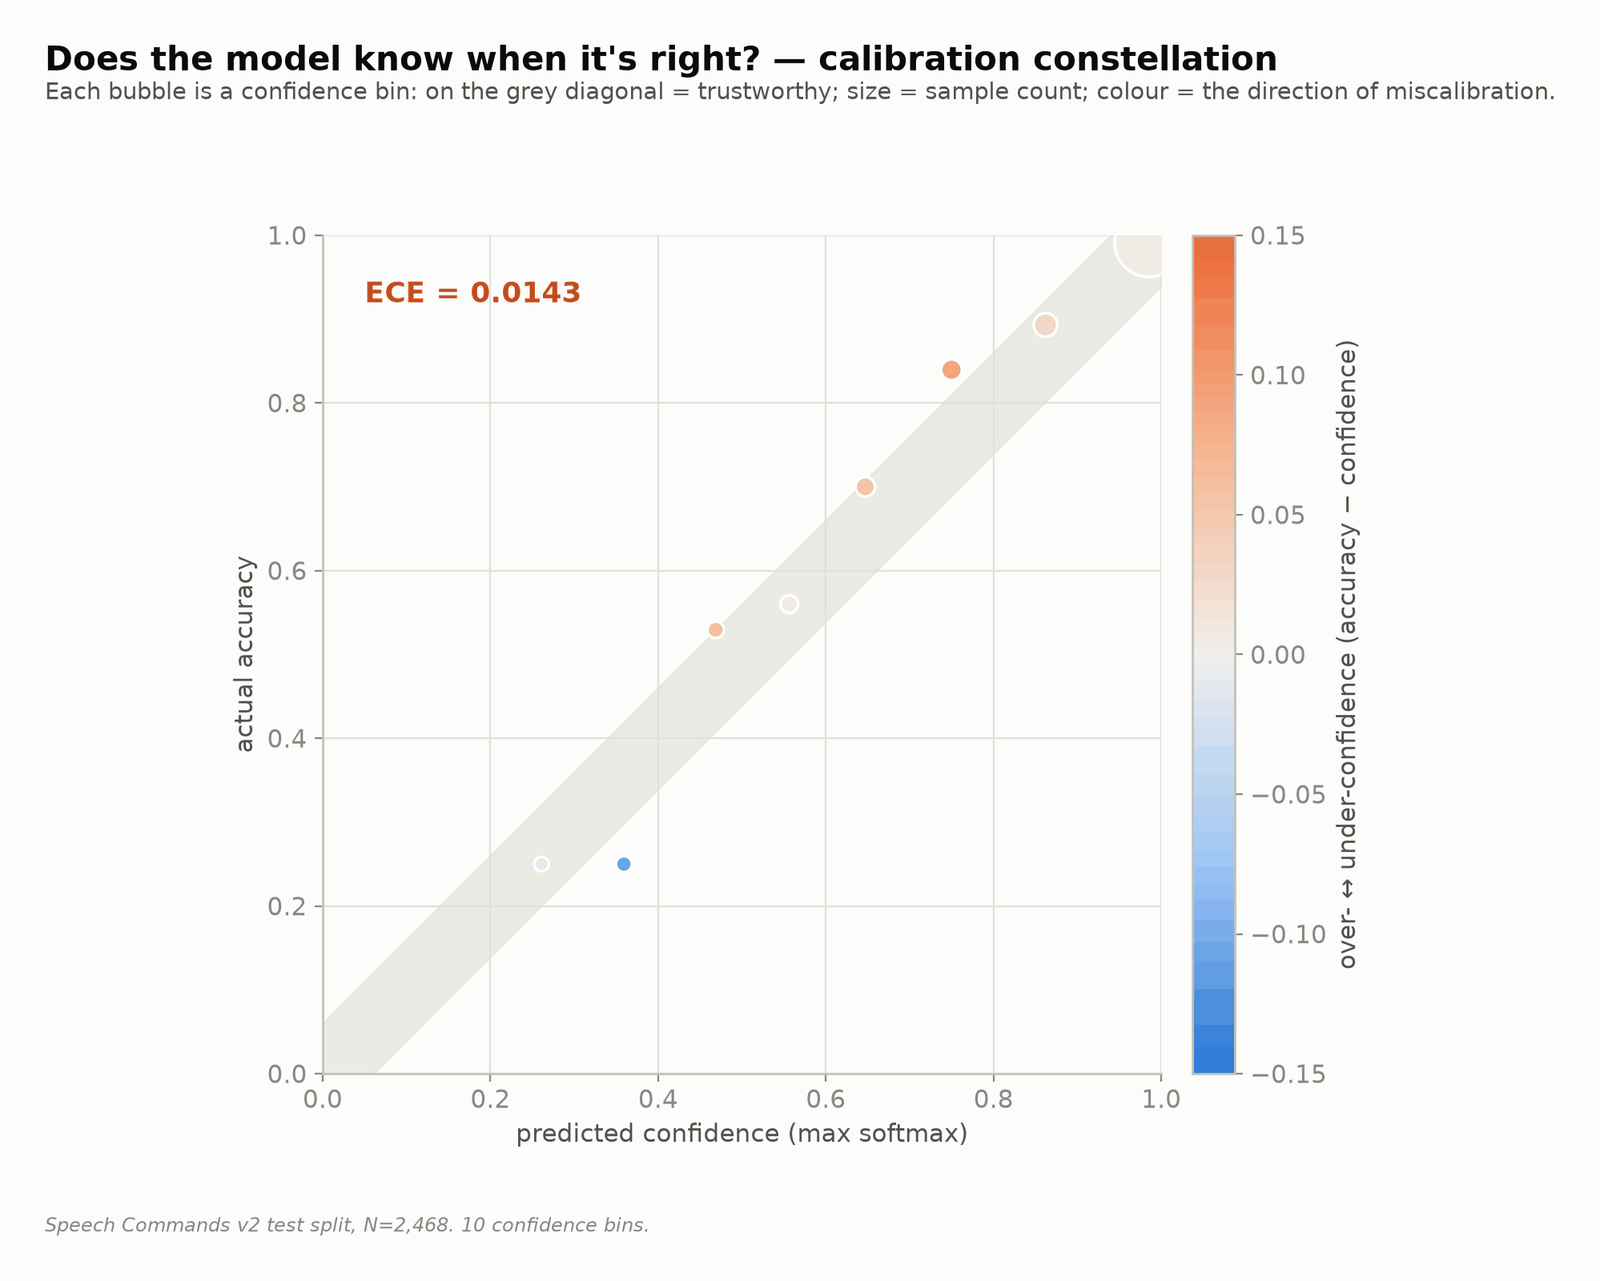
\includegraphics[width=\linewidth]{figures/voice_V3_constellation.png}
\caption{Calibration constellation --- confidence bins as bubbles against observed accuracy on the honesty diagonal.}
\label{fig:36}
\end{figure}

Expected calibration error by \EQREF{150} over fifteen bins is

\begin{equation}
\label{eq:254}
\begin{aligned}
\mathrm{ECE} = 1.54 \% , \mathbb{E}[ \text{conf}\; | \;\text{correct} ] = 0.950 , \\
\mathbb{E}[ \text{conf}\; | \;\text{error} ] = 0.640 ,
\end{aligned}
\end{equation}

with macro one-versus-rest ROC-AUC 0.9961 and log-loss 0.1644. Selective prediction with a reject option is therefore available, and the risk--coverage pairs of \EQREF{133} are

\begin{equation}
\label{eq:255}
\begin{aligned}
\zeta = 0.7: \mathrm{cov} = 92.2 \% , \\
\mathrm{Acc} = 97.72 \% ; \zeta = 0.9: \mathrm{cov} = 81.5 \% , \\
\mathrm{Acc} = 99.10 \% .
\end{aligned}
\end{equation}

The honest comparison is nonetheless unfavourable. Matching the baseline's 99.45 \% precision requires

\begin{equation}
\label{eq:256}
\begin{aligned}
\zeta = 0.965 , \\
\mathrm{cov} = 68.9 \% \mathrm{against} \;\text{the baseline}\;'s \mathrm{cov}_R = 96.0 \% ,
\end{aligned}
\end{equation}

so the proposed network \emph{can} adopt the abstention strategy but attains a markedly worse risk--coverage curve. This, rather than the headline accuracy, is the substantive gap between the two systems. It also gives the deployment rule a defensible setting: a $\zeta$ = 0.7 gate costs 7.8 \% coverage and removes roughly half the substitution risk, and by the Chow rule following \EQREF{134} this corresponds to an implied cost ratio $c_{\mathrm{sub}}$/$c_{\mathrm{abs}}$ $\approx$ 3.3, which is a defensible valuation for an interface in which an unintended command may require several actions to undo.

\FIGREF{37} decomposes confidence by keyword.

\begin{figure}[pos=htbp]
\centering
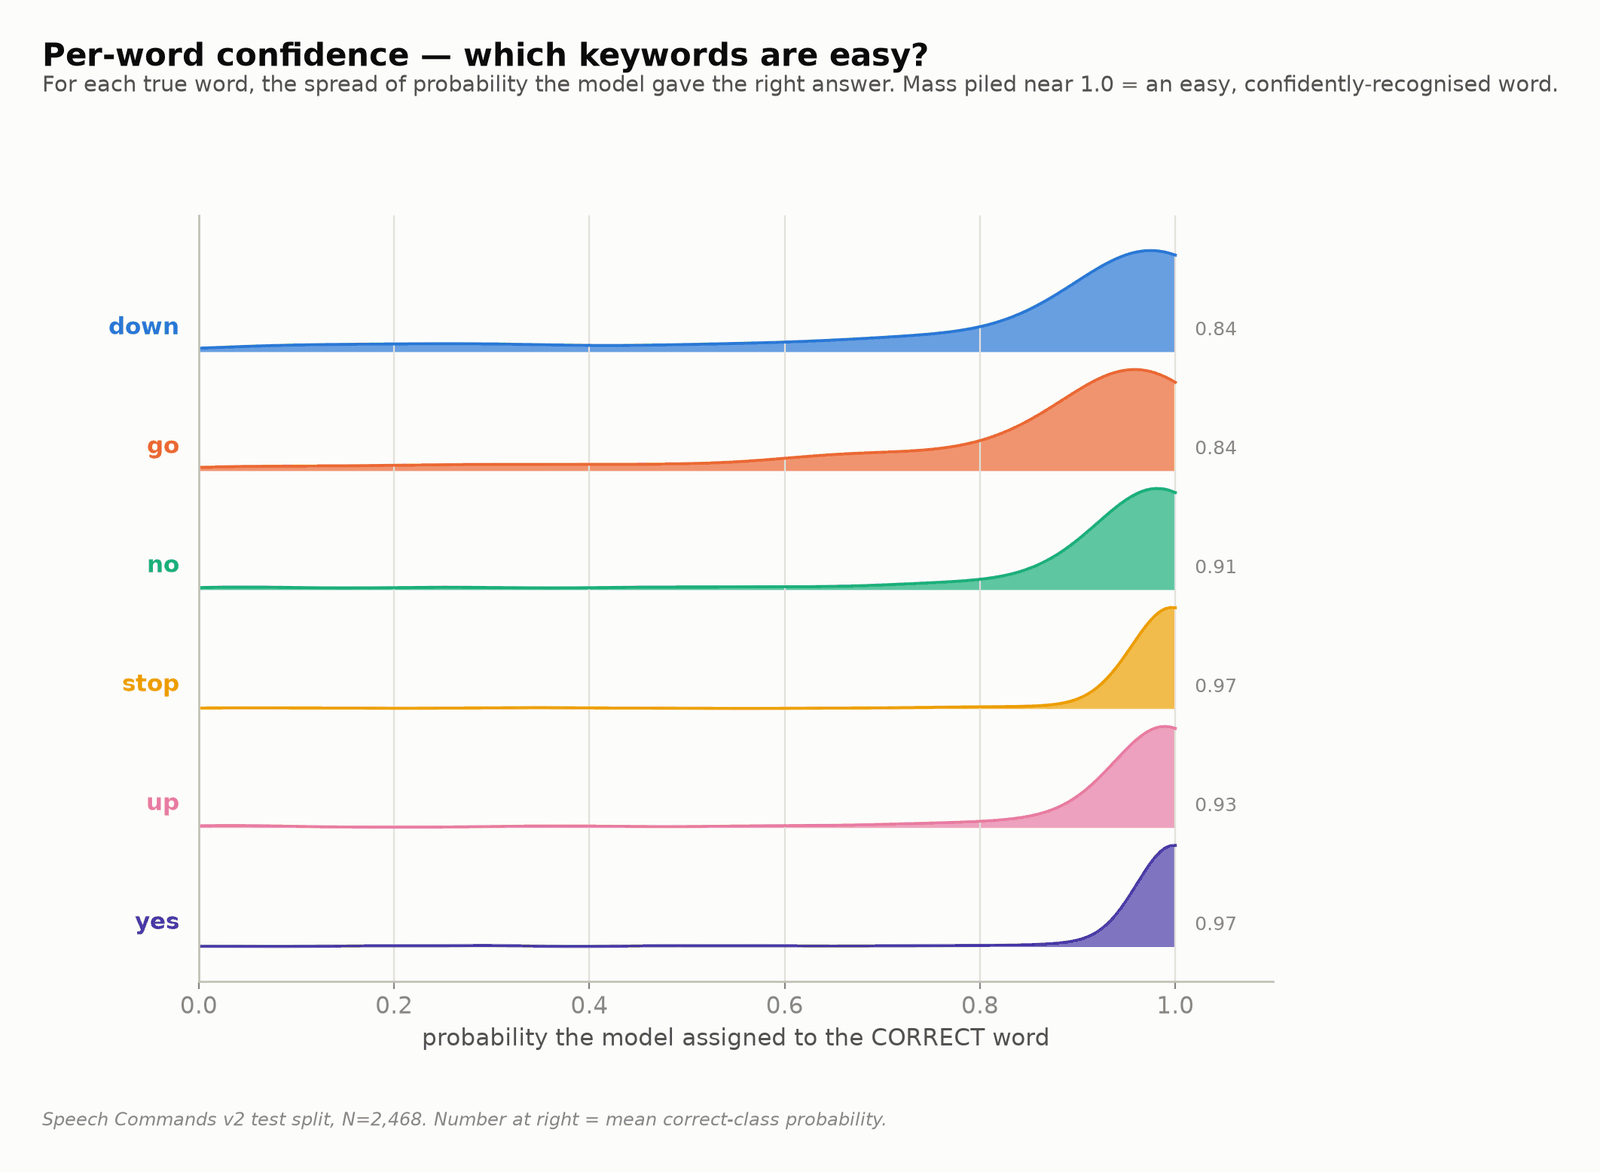
\includegraphics[width=\linewidth]{figures/voice_V4_perword_ridgeline.png}
\caption{Per-word confidence --- the distribution of predicted probability assigned to the correct class, per keyword.}
\label{fig:37}
\end{figure}

One-versus-rest AUC orders as

\begin{equation}
\label{eq:257}
\text{yes}\; 0.9997 > \;\text{stop}\; 0.9992 > up 0.9984 > no 0.9959 > \;\text{down}\; 0.9941 > go 0.9896 ,
\end{equation}

and the ordering is acoustic, not statistical: class frequencies span only 402--425 clips, so prior imbalance explains none of the spread,

\begin{equation}
\label{eq:258}
\mathrm{max}_c n_c / \mathrm{min}_c n_c = 425/402 = 1.057 .
\end{equation}

The two strongest carry unvoiced fricative or plosive energy --- the /s/ of \emph{yes}, the /st/ cluster of \emph{stop} --- producing a high-frequency signature unique among the six and sharply localised in time, hence concentrated in the upper mel bands of \EQREF{31} and a narrow span of time frames. The weakest, \emph{go}, is a single voiced plosive with a sustained vowel and no coda: the shortest window of class-discriminative evidence in the vocabulary. This is the quantitative basis for the rebinding recommendation of \FIGREF{34} --- the network's weakness is inherited from the label set, so changing the label set is the correct intervention.

\FIGREF{38} quantifies separability independently of any threshold.

\begin{figure}[pos=htbp]
\centering
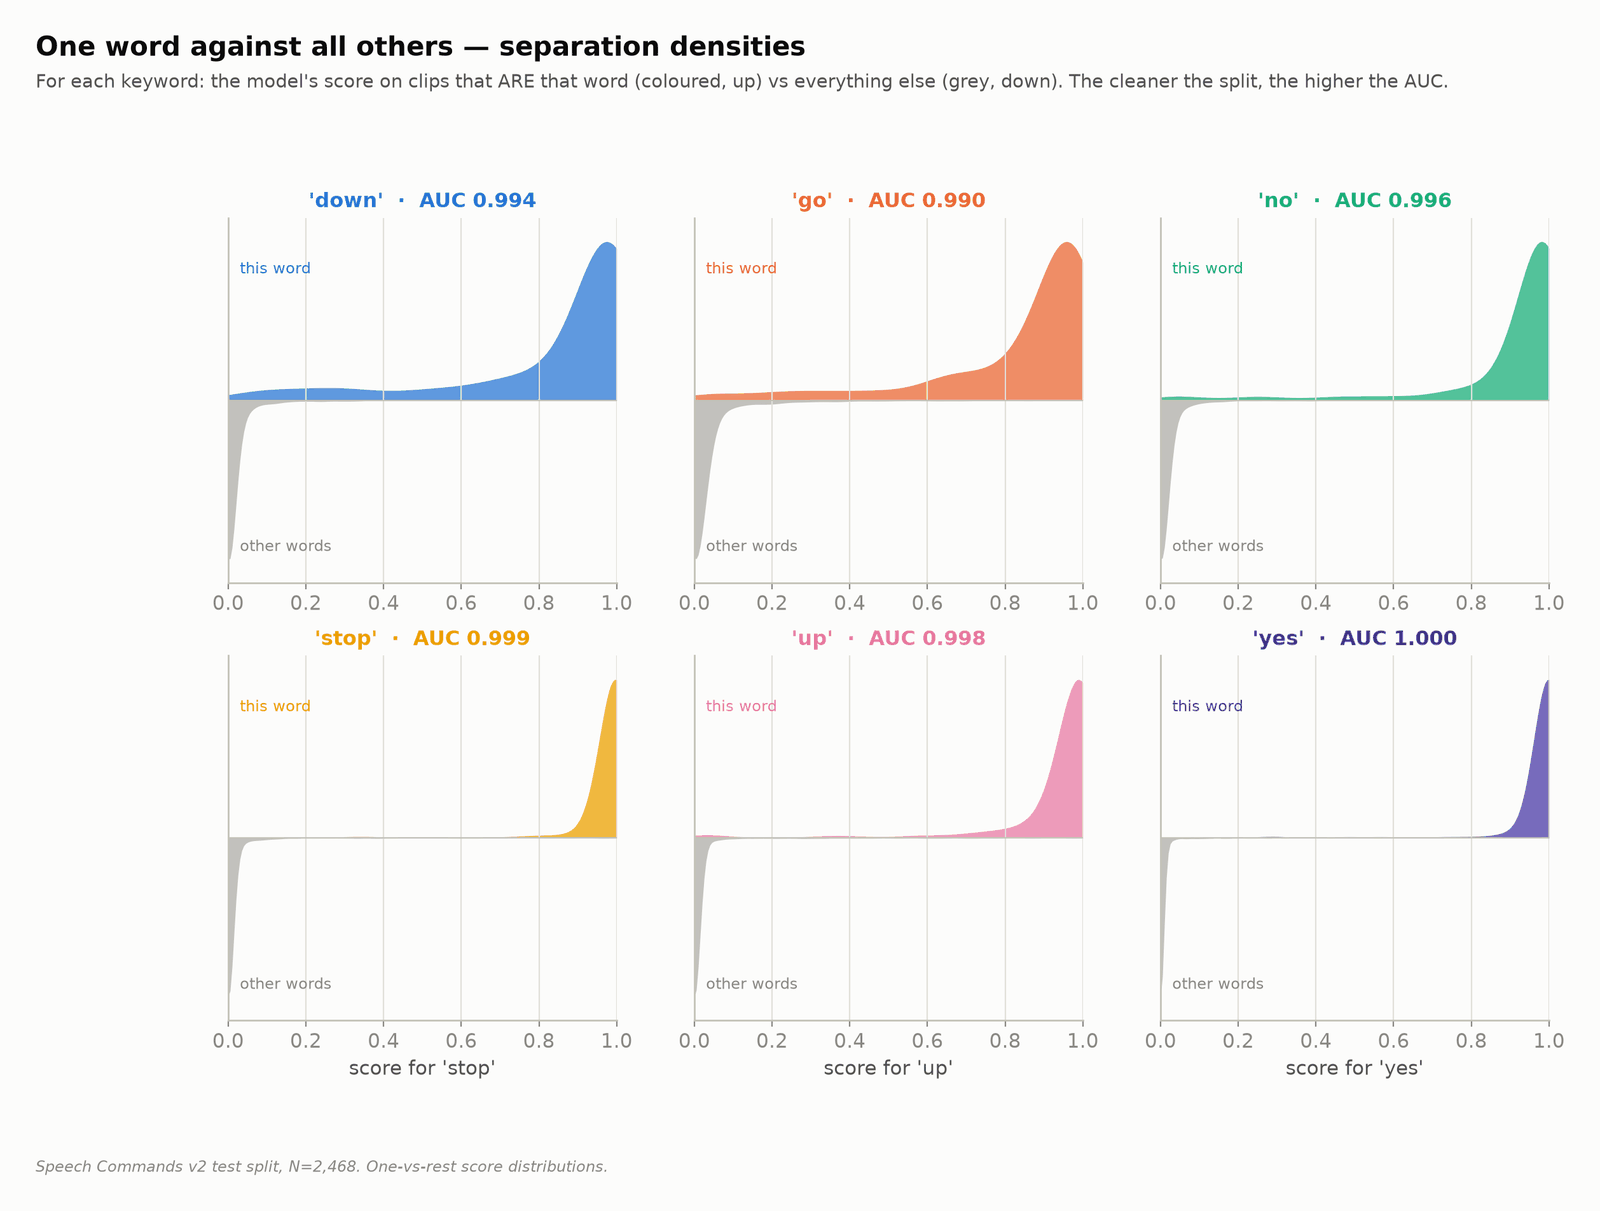
\includegraphics[width=\linewidth]{figures/voice_V5_separation.png}
\caption{Separation densities --- per keyword, the score distribution on target clips against all others, with AUC.}
\label{fig:38}
\end{figure}

Every keyword exceeds 0.989 AUC, so all six classes are near-separable in the learned latent space at the ranking level, while operating-point accuracy is 94.53 \%. The gap between the two,

\begin{equation}
\label{eq:259}
\mathbb{E}_c[ \mathrm{AUC}_c ] = 0.9962 \mathrm{against} \mathrm{Acc} = 0.9453 ,
\end{equation}

localises the residual error in \textbf{threshold placement and class-boundary geometry} rather than in feature learning. This is the diagnostic that separates a model needing capacity from one needing decision logic, and it places this network unambiguously in the second category. It is also why the confidence gate of \EQREF{255} lifts accuracy to 99.10 \% without touching a weight.

\FIGREF{39} examines the decision margin.

\begin{figure}[pos=htbp]
\centering
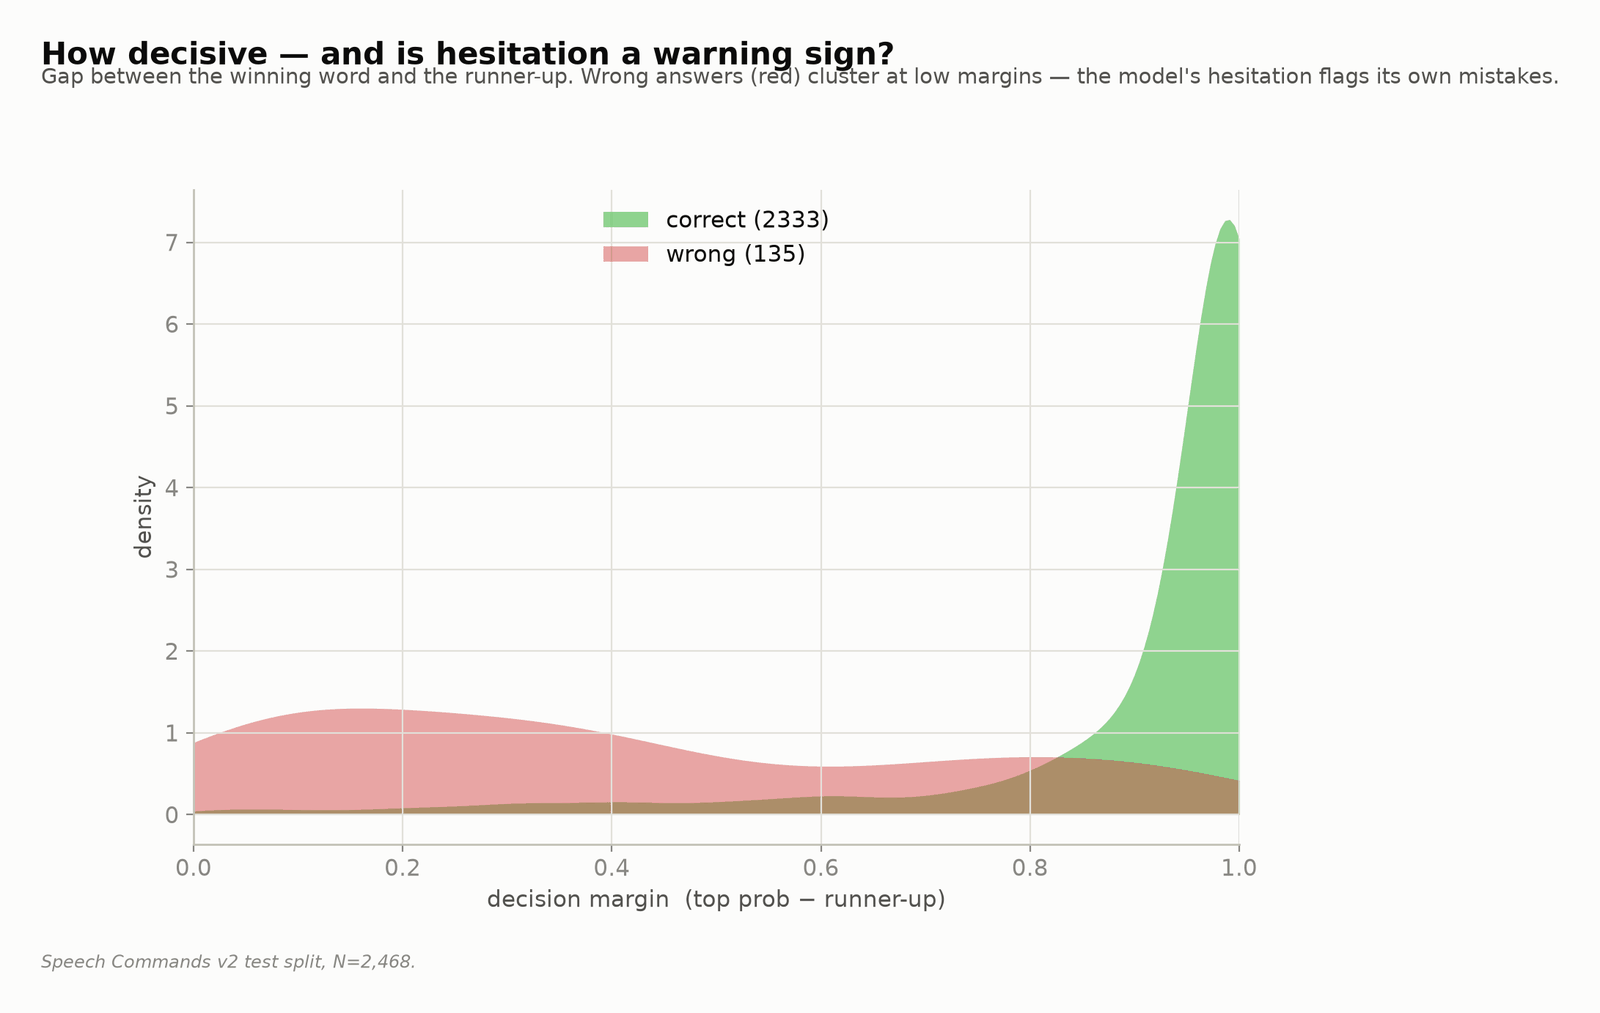
\includegraphics[width=\linewidth]{figures/voice_V6_decision_margin.png}
\caption{Decision margin --- the gap between the top two class probabilities, for correct against incorrect predictions.}
\label{fig:39}
\end{figure}

Defining the margin

\begin{equation}
\label{eq:260}
m(x) = p_{(1)}(x) - p_{(2)}(x) ,
\end{equation}

the measured means are 0.912 on correct predictions and 0.404 on errors, so errors carry measurable internal hesitation and are detectable at runtime from logits already computed. A useful negative result attaches: as an error detector the margin achieves AUC 0.930 against 0.932 for top-1 confidence,

\begin{equation}
\label{eq:261}
| \mathrm{AUC}_{\mathrm{margin}} - \mathrm{AUC}_{\mathrm{conf}} | = 0.002 ,
\end{equation}

statistically indistinguishable at this sample size, so the theoretical advantage of margin over confidence --- invariance to overall distribution sharpness --- does not materialise here. The simpler top-1 gate of \EQREF{132} is the correct implementation choice, and a margin-based gate would add complexity for nothing measurable.

\FIGREF{40} gives the aggregate flow.

\begin{figure}[pos=htbp]
\centering
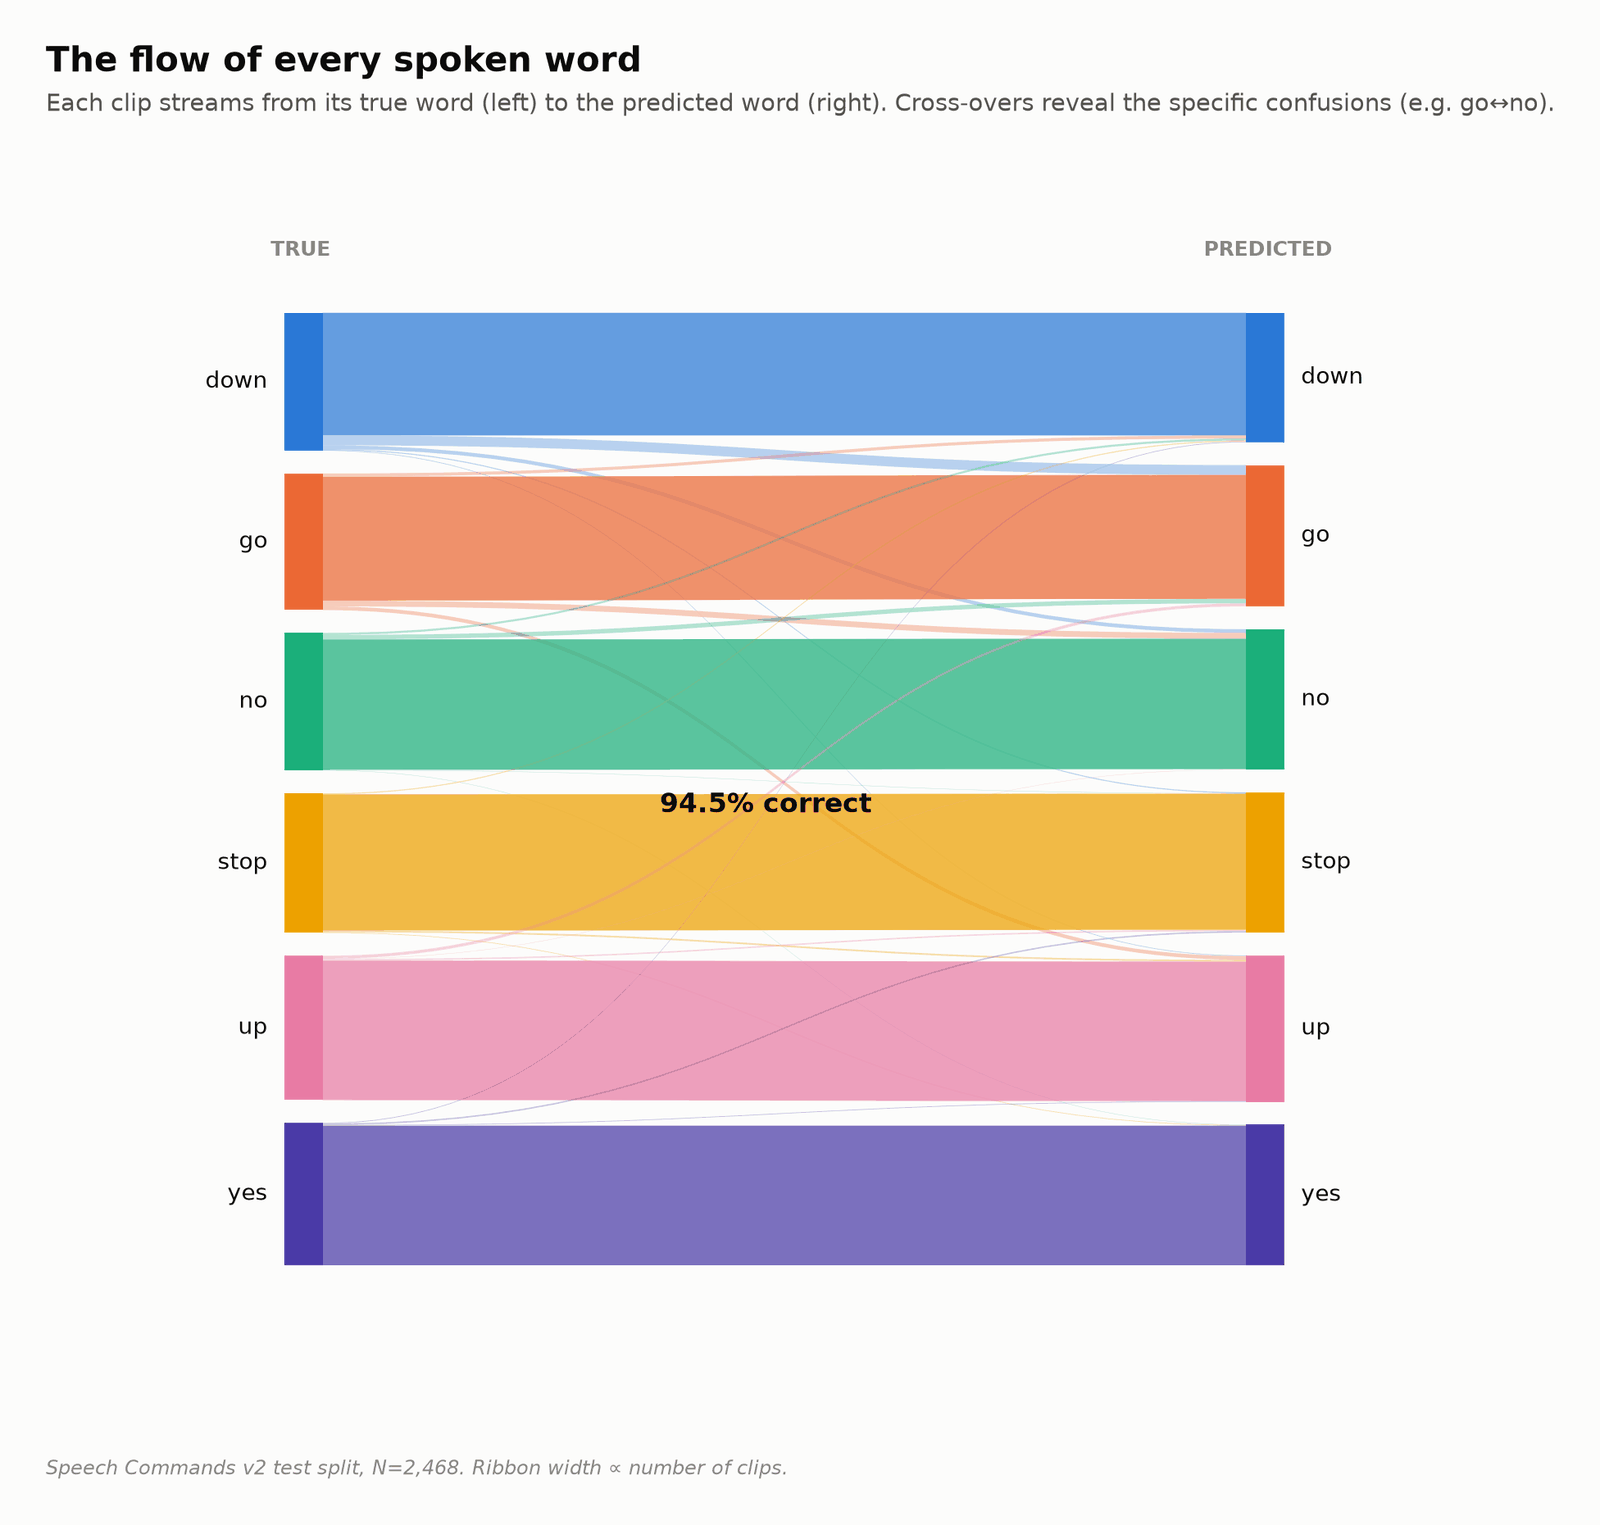
\includegraphics[width=\linewidth]{figures/voice_V7_word_flow.png}
\caption{Word flow --- every clip streaming from its true keyword to its predicted keyword; crossings are confusions.}
\label{fig:40}
\end{figure}

Misrouting concentrates in a few thick ribbons and the confusion graph is sparse. Treating the confusion counts as a weighted graph on the six keywords, the edge density is

\begin{equation}
\label{eq:262}
\text{density}\; = |{ (c, c') : N_{c\to c'} > 0, c \neq c' }| / ( C(C-1) ) \ll 1 ,
\end{equation}

with most keyword pairs exchanging no clips at all. Sparsity matters more than total error mass for interface design, because a sparse graph is remediable by vocabulary substitution or by a targeted pairwise discriminator over three pairs, both far cheaper than retraining the six-way classifier. A dense graph of identical error mass would admit neither remedy --- which is what makes the recommendation of \FIGREF{34} available at all.

\FIGRANGE{41}{44} re-render the same predictions, testing the sparsity and confidence-separation claims as joint structure.

\begin{figure}[pos=htbp]
\centering
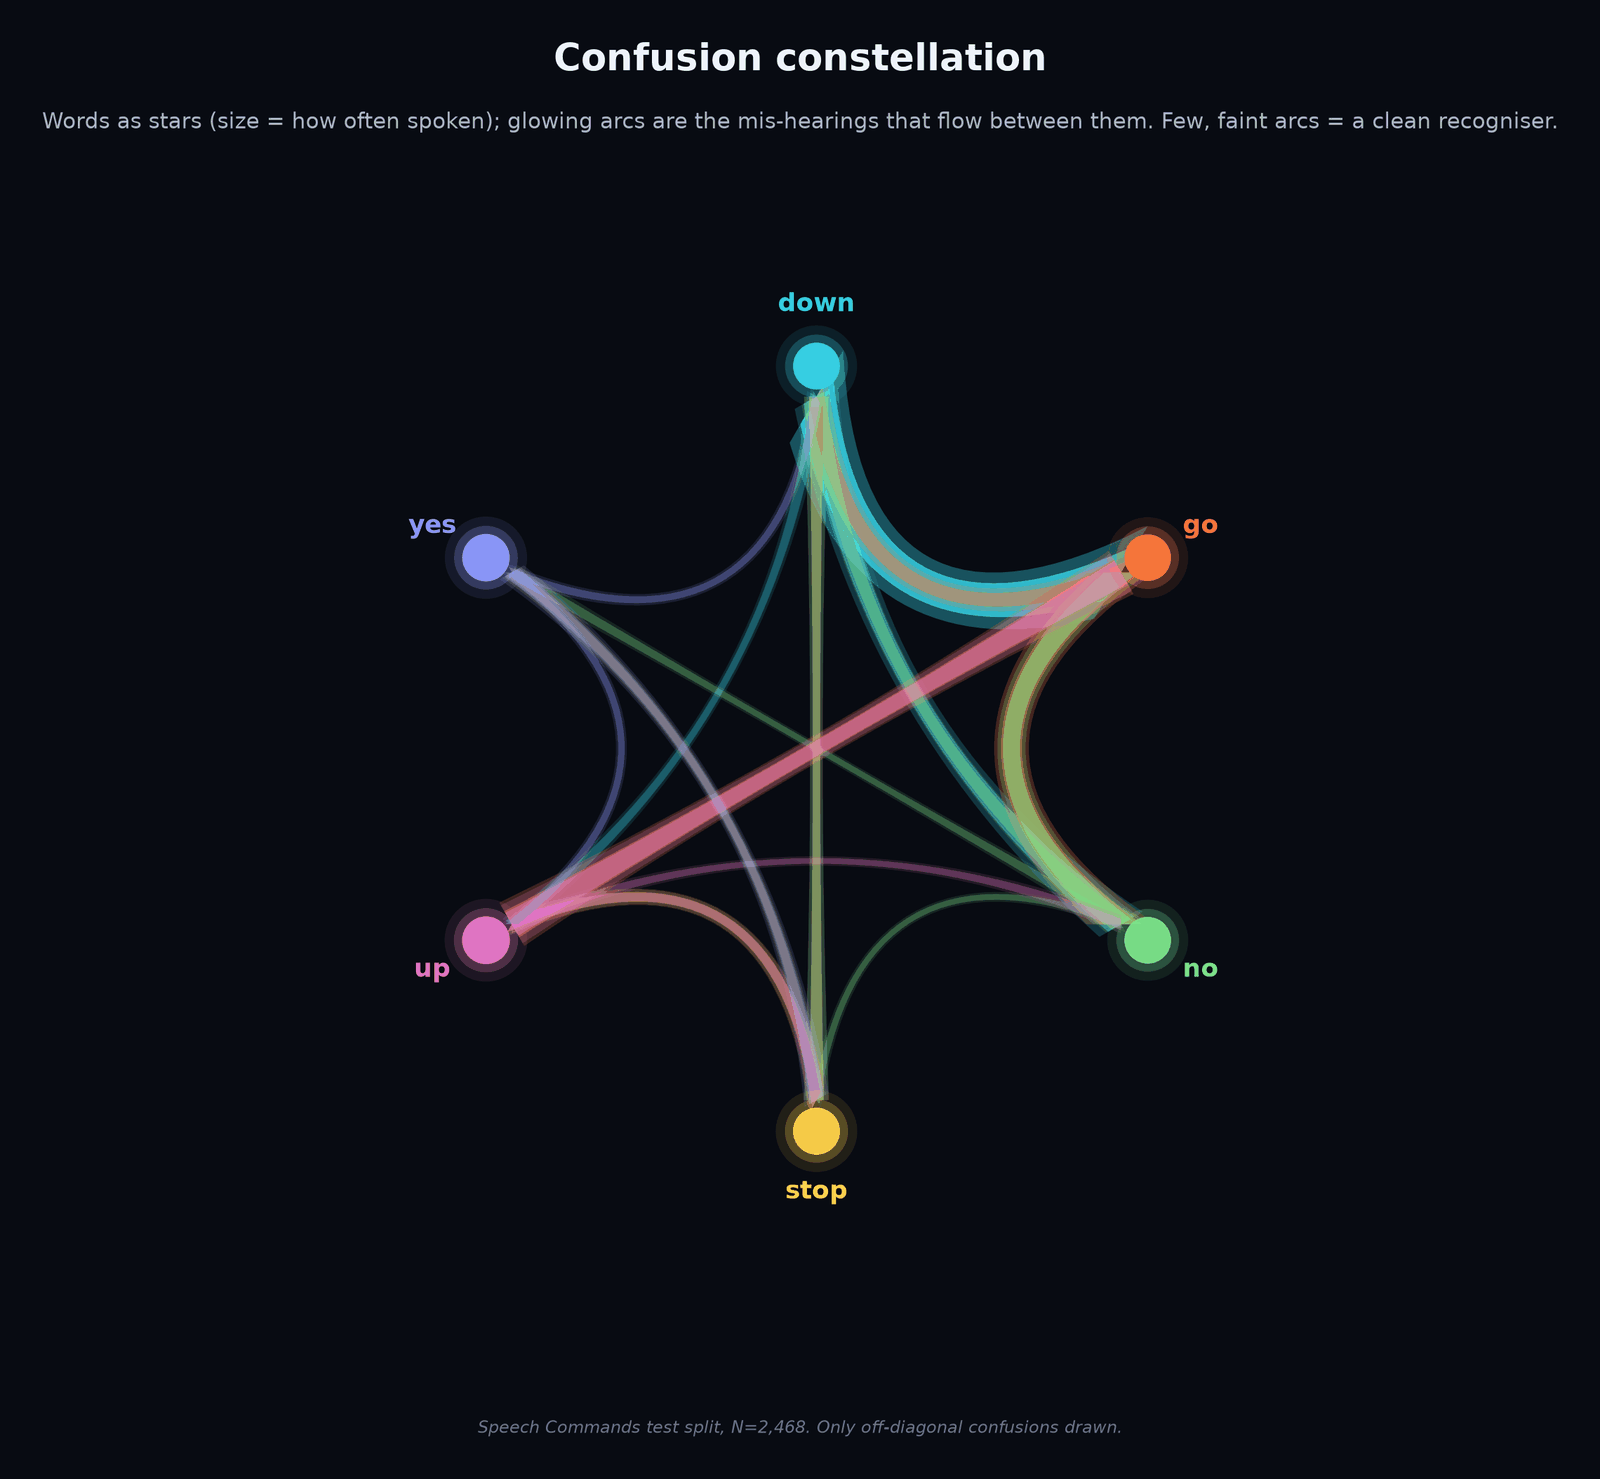
\includegraphics[width=\linewidth]{figures/figures_art_voice_VA1_chord.png}
\caption{Confusion constellation --- keywords as nodes sized by frequency, with arcs carrying the misrecognised clips between them.}
\label{fig:41}
\end{figure}

Rendering confusion as connectivity shows that of fifteen possible undirected pairs, three carry 63 \% of the 135 errors while several carry none, and that the three loaded arcs form a \textbf{connected triangle} among the back-vowel words \{\emph{down}, \emph{go}, \emph{no}\}. That is a stronger statement than pairwise confusion: it identifies a single phonetic neighbourhood as the locus of all significant uncertainty. Removing one vertex from a triangle removes two of its three edges, which is why one substitution inside that triangle reduces total error disproportionately ---

\begin{equation}
\label{eq:263}
\Delta \;\text{error}\; \geq ( 38 + 30 ) / 135 = 50.4 \% \;\text{if}\; \;\text{go is rebound} ,
\end{equation}

against the 28 \% that removing an arbitrary single edge would achieve. The graph structure, not the error count, is what makes the remedy identifiable.

\begin{figure}[pos=htbp]
\centering
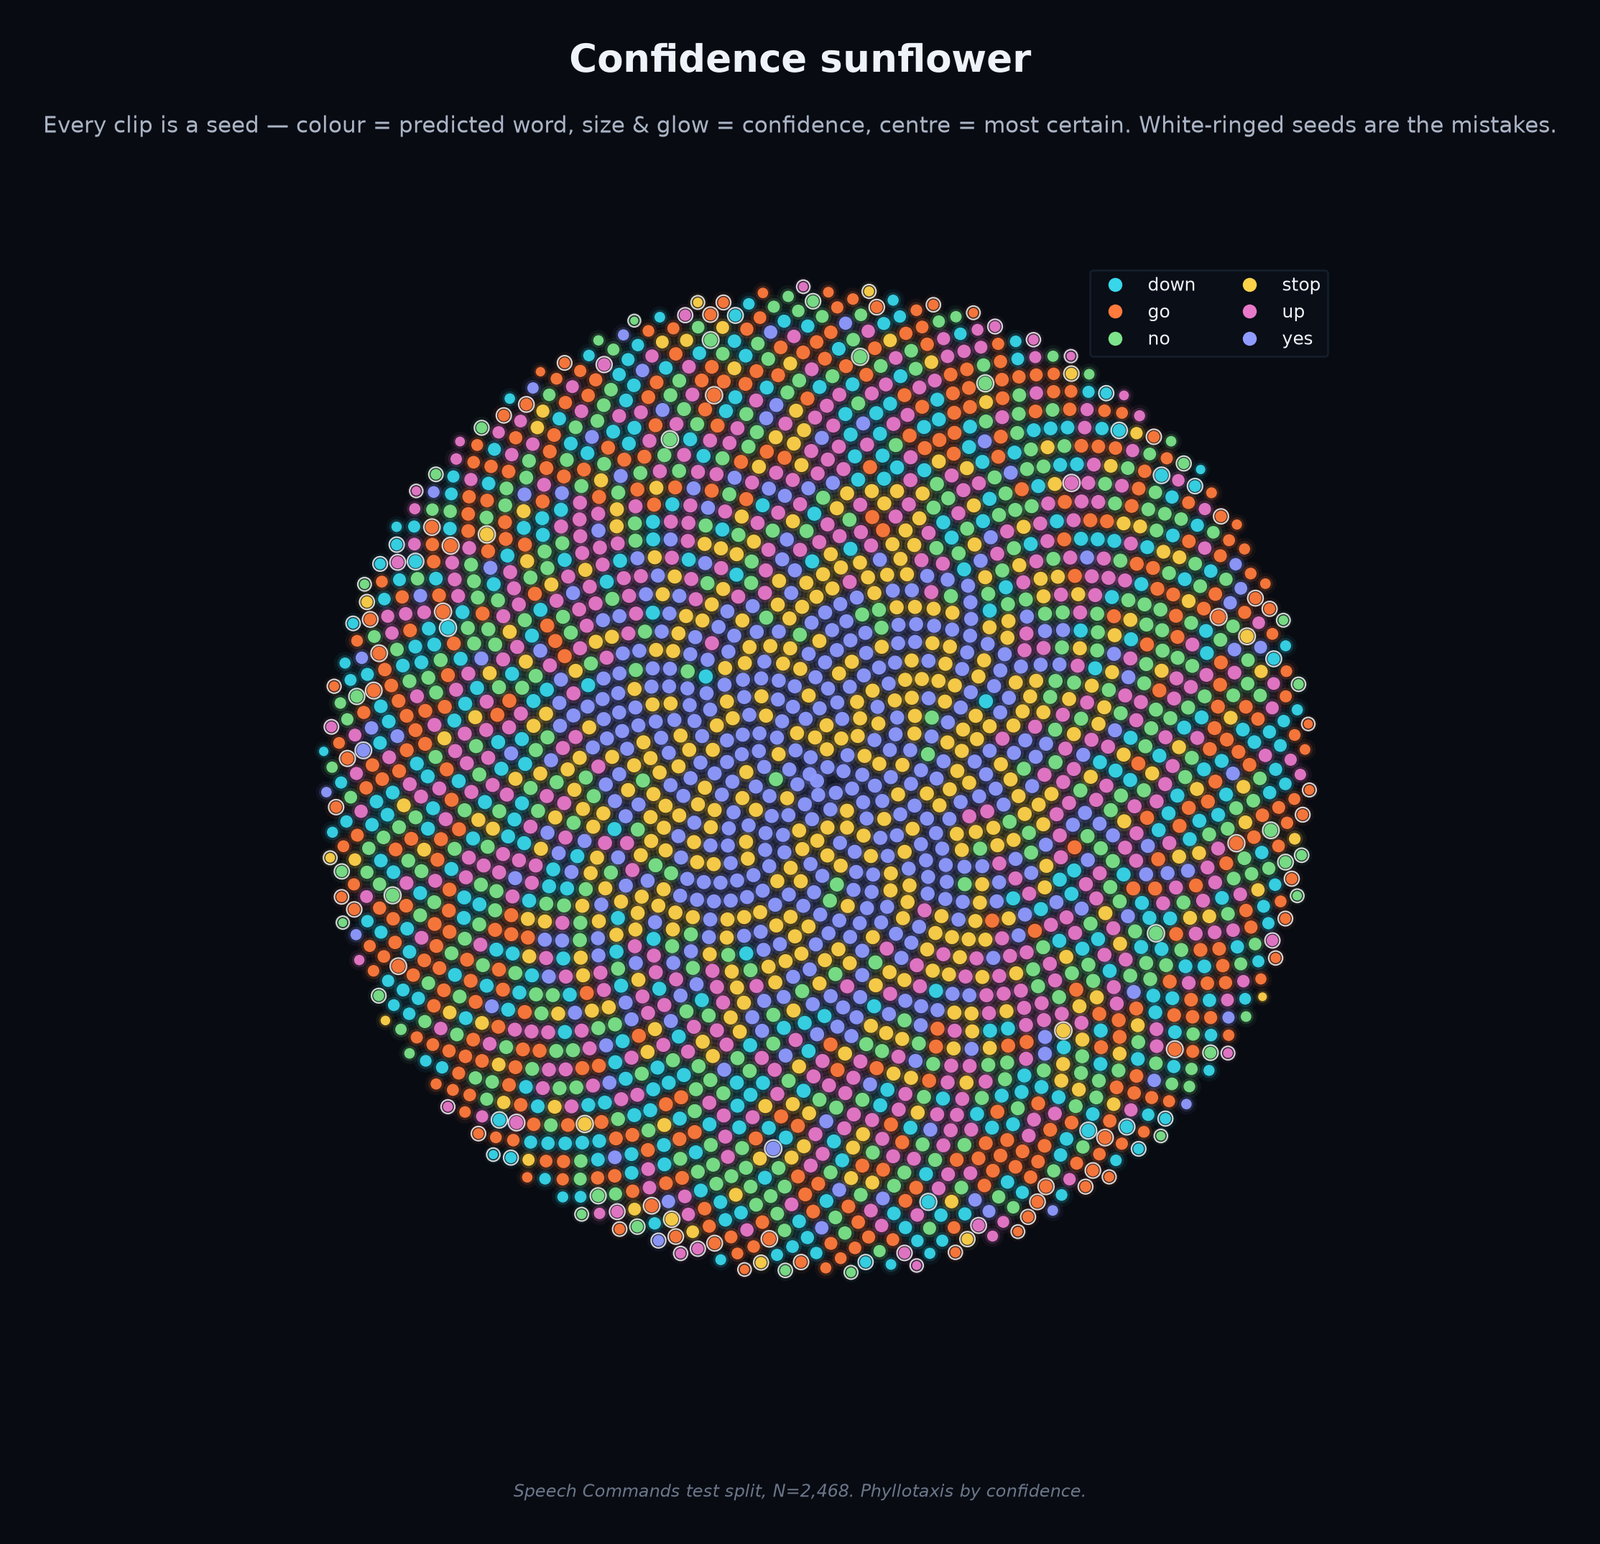
\includegraphics[width=\linewidth]{figures/figures_art_voice_VA2_sunflower.png}
\caption{Confidence sunflower --- every test clip as a seed, coloured by predicted keyword and sized by confidence, with misclassified clips ringed.}
\label{fig:42}
\end{figure}

Ringed seeds are systematically small, the per-clip form of the 0.950 against 0.640 confidence separation of \EQREF{254}. The informative population is the exception: large ringed seeds are confidently wrong clips that no gate can intercept. Their scarcity relative to small ringed seeds is quantified by the 0.932 error-detection AUC of \FIGREF{39} and is what makes the operating points of \EQREF{255} achievable --- a model with identical accuracy but poorer confidence separation would admit no selective regime at all, and the abstention comparison with the ASR baseline could not even be posed.

\begin{figure}[pos=htbp]
\centering
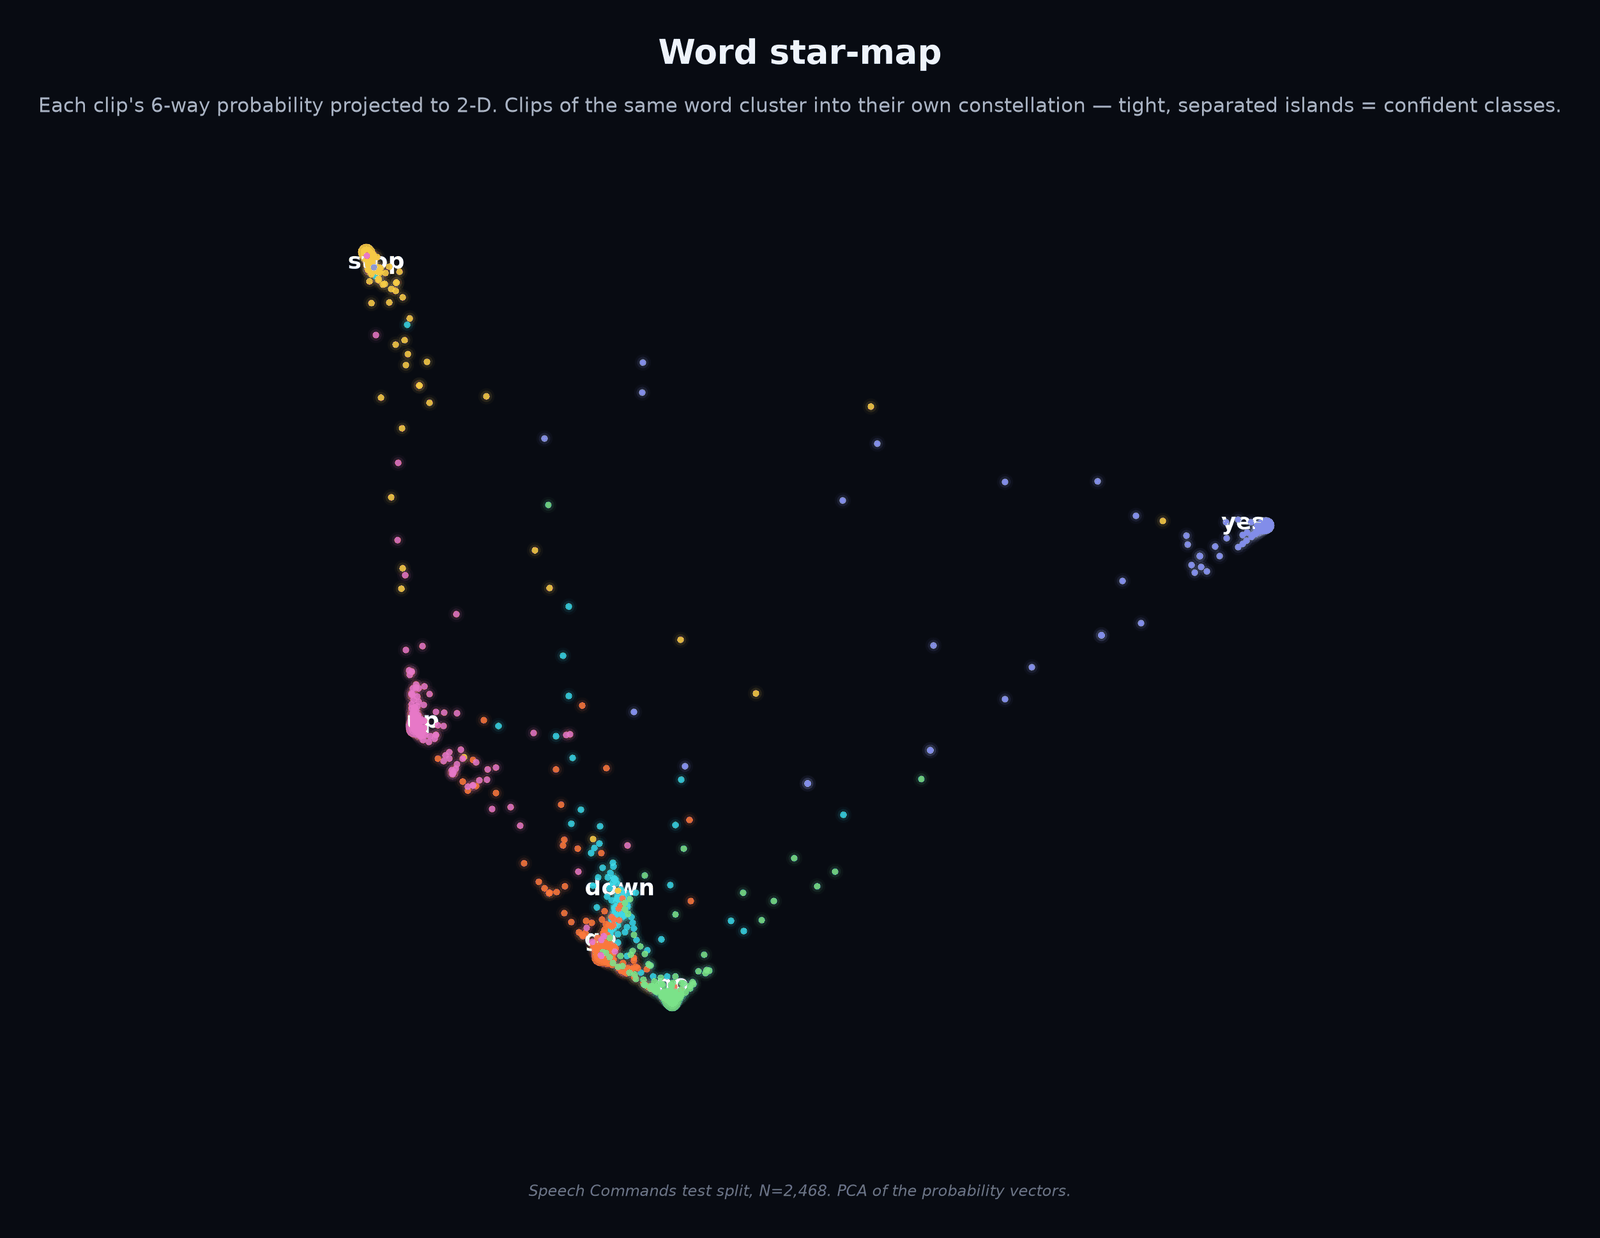
\includegraphics[width=\linewidth]{figures/figures_art_voice_VA3_starmap.png}
\caption{Word star-map --- each clip's six-way probability vector projected to two dimensions; tight islands indicate confidently separated classes.}
\label{fig:43}
\end{figure}

Projecting the output simplex $\Delta^{5}$ = \{ p $\in$ $\mathbb{R}^{6}_{+}$ : $\Sigma$ $p_{c}$ = 1 \} to two dimensions visualises decision geometry directly. Six islands resolve, consistent with all per-word AUCs exceeding 0.989, and their tightness follows the AUC ordering \EQREF{257} --- \emph{yes} and \emph{stop} most compact, \emph{go} most diffuse and most overlapped with its neighbours. Because the projection is of the \emph{probability vector} rather than an internal embedding, island overlap corresponds directly to realisable confusion at the decision boundary, connecting latent geometry to the confusion structure of \FIGREF{34} without an intervening assumption.

\begin{figure}[pos=htbp]
\centering
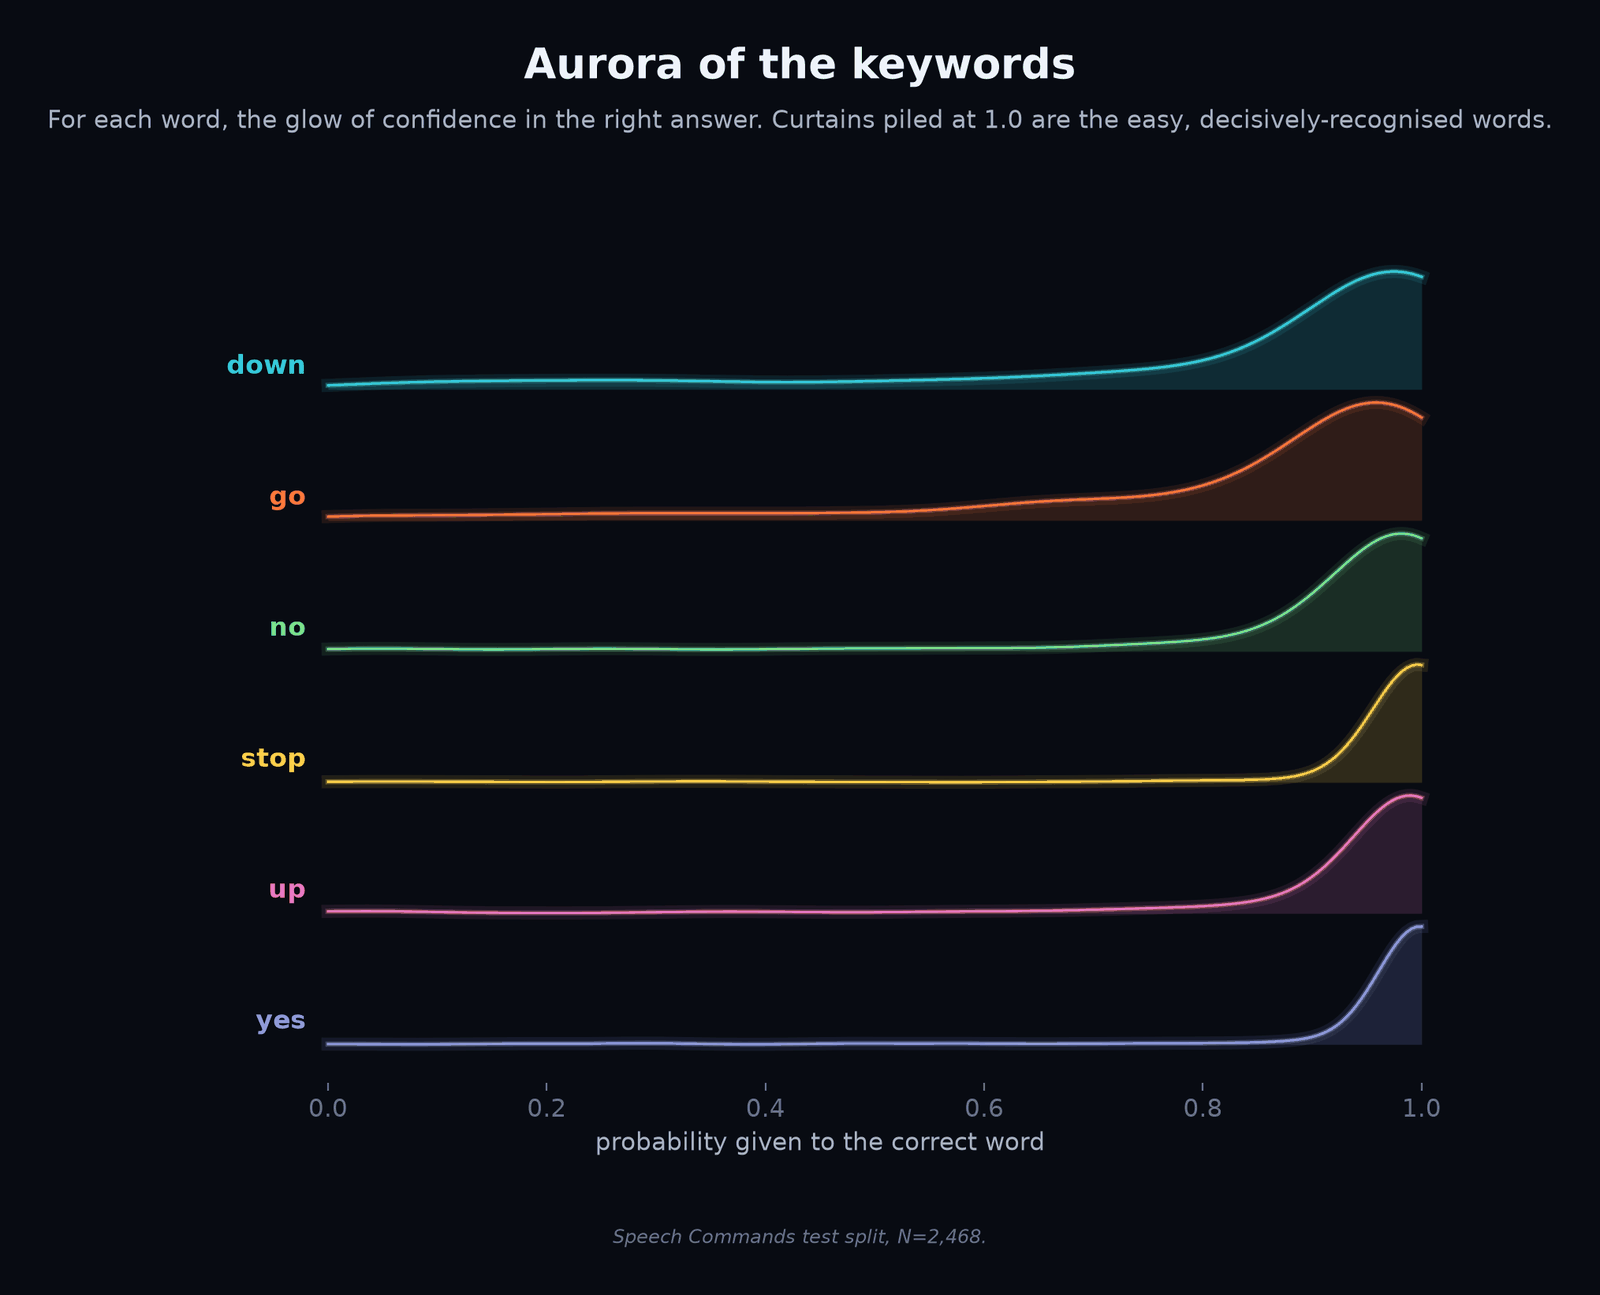
\includegraphics[width=\linewidth]{figures/figures_art_voice_VA4_aurora.png}
\caption{Aurora of the keywords --- per keyword, the density of probability assigned to the correct class.}
\label{fig:44}
\end{figure}

The curtains rank as the per-class F$_{1}$ scores do,

\begin{equation}
\label{eq:264}
\text{yes}\; 0.987 > \;\text{stop}\; 0.973 > up 0.960 > no 0.939 > \;\text{down}\; 0.917 > go 0.892 ,
\end{equation}

while class frequencies span only 402--425 clips by \EQREF{258}, so frequency explains none of the spread and phonetic distinctiveness explains all of it. This is the cleanest available statement that residual voice error is a property of the chosen command vocabulary --- addressable by vocabulary design at zero computational cost rather than by additional capacity, which for a system budgeted at 101,766 parameters by \EQREF{84} is the difference between a solvable and an unsolvable problem.

\subsubsection{What the network listens to}

\begin{figure}[pos=htbp]
\centering
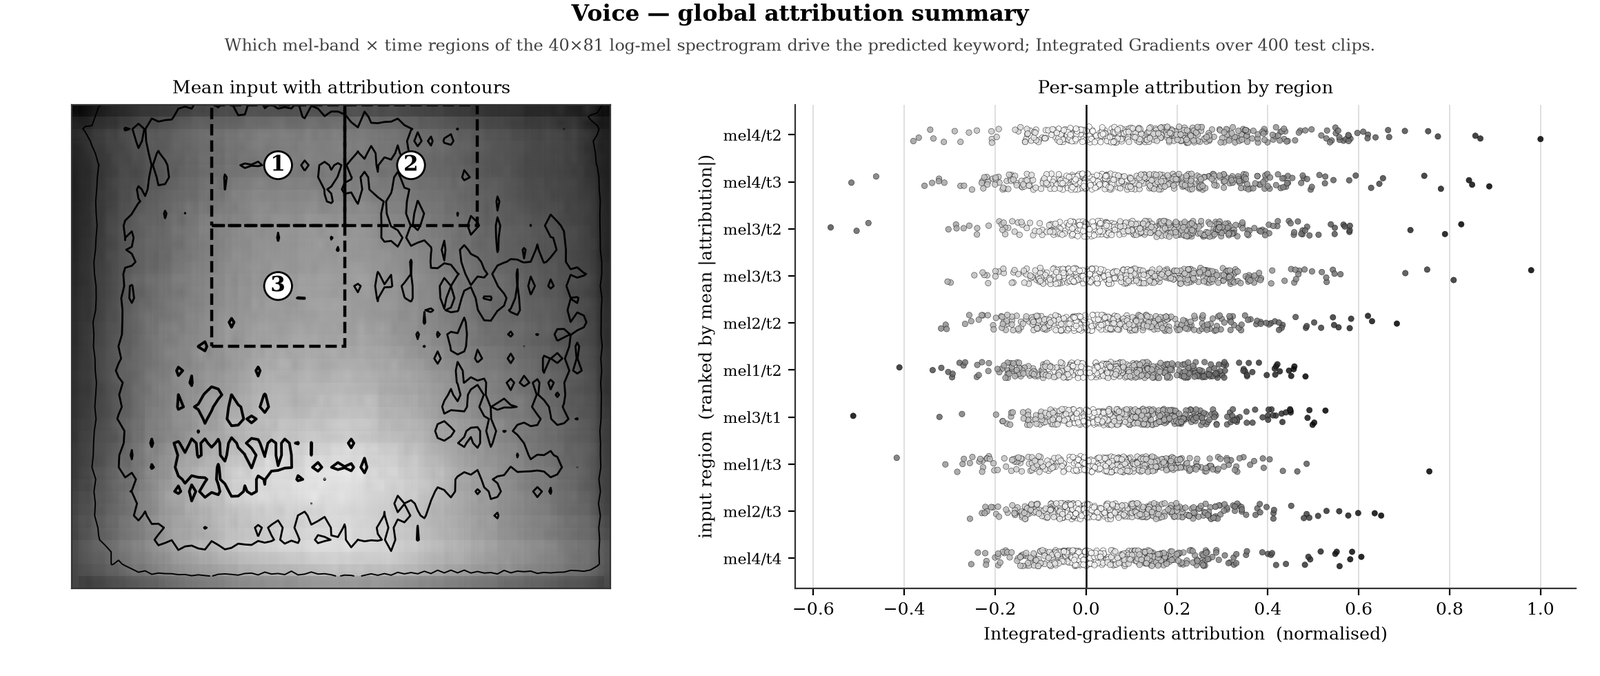
\includegraphics[width=\linewidth]{figures/attribution_voice_A1_summary.png}
\caption{Voice --- global attribution summary over the 40 $\times$ 81 log-mel spectrogram, regions indexed by mel band and time slot.}
\label{fig:45}
\end{figure}

Attribution concentrates in the upper mel bands (mel3, mel4) during central time slots (t2, t3), with negligible contribution from the lowest bands and the leading and trailing slots. The network therefore learned an \textbf{implicit voice-activity gate}: Speech Commands clips are one second long by \EQREF{27} with the utterance roughly centred and silence-padded, and the model learned to discard the padding without being told where the word begins. Writing the region attribution as a separable product,

\begin{equation}
\label{eq:265}
\begin{aligned}
\mathrm{Attr}( b, \tau ) \approx \omega (b) \cdot g(\tau ) , \\
g(\tau ) \approx 0 \;\text{for}\; \tau \;\text{in the leading and trailing slots} ,
\end{aligned}
\end{equation}

the temporal factor g is the gate and the spectral factor $\omega$ the evidence weighting. Both matter for deployment: g is why the network transfers to a live microphone stream whose padding statistics differ from the corpus, and $\omega$ --- concentrated in the high-frequency bands carrying fricative and plosive energy --- is the mechanistic counterpart of the AUC ordering \EQREF{257} and the reason \emph{go}, whose discriminative energy is a brief low-frequency transient, is weakest.

\begin{figure}[pos=htbp]
\centering
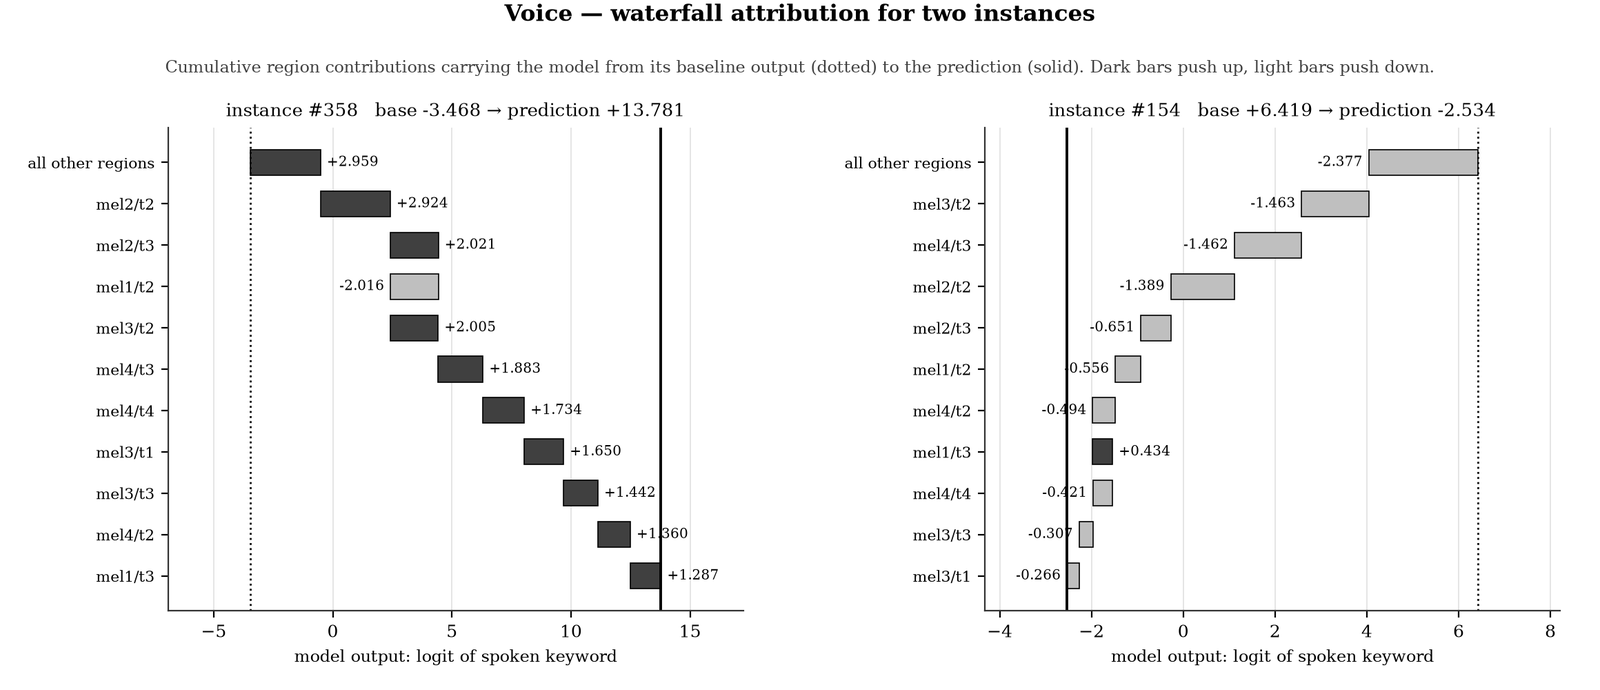
\includegraphics[width=\linewidth]{figures/attribution_voice_A2_waterfall.png}
\caption{Voice --- waterfall attribution for two extreme instances of the predicted keyword.}
\label{fig:46}
\end{figure}

Per-instance decompositions are dominated by two or three time-localised high-band regions, so classification rests on short sparse spectro-temporal events rather than integration over the clip. Writing the effective support as

\begin{equation}
\label{eq:266}
| \;\text{supp}\;( \mathrm{Attr} ) | / |\mathcal{R}| \approx 3/16 = 0.19 ,
\end{equation}

this sparsity is what permits 101,766 parameters to reach 94.53 \% at 2.7 ms per clip --- an efficiency result with an explanation rather than an empirical accident, since by \EQREF{78} global average pooling discards spatial extent precisely because the evidence is sparse and its location is not informative. It also predicts the failure mode: where the discriminative event is short and low-energy, as for \emph{go}, the margin \EQREF{260} collapses, which is exactly what \FIGREF{39} measures and \FIGREF{34} localises.

\begin{figure}[pos=htbp]
\centering
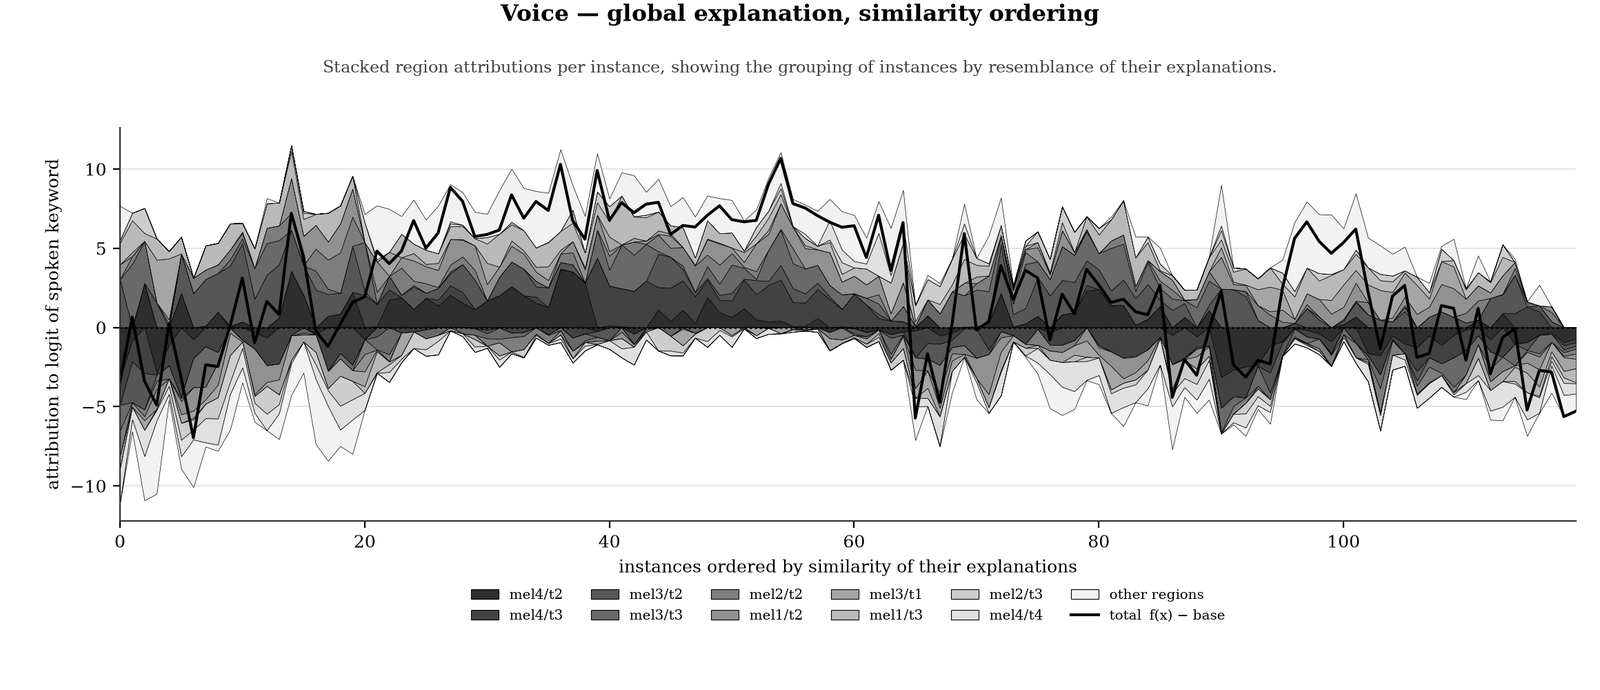
\includegraphics[width=\linewidth]{figures/attribution_voice_A3_similarity.png}
\caption{Voice --- global explanation under similarity ordering.}
\label{fig:47}
\end{figure}

Similarity ordering produces clearly separated blocks, in contrast to the continua of gaze and head pose. This is the expected structure for a categorical task --- the explanation map \EQREF{217} is Lipschitz with respect to a \emph{discrete} label metric rather than a continuous target --- and it is a cross-check that the ordering reflects task structure rather than an artefact of the method. Each block corresponds to clips explained by the same regions, and clips at block boundaries are candidates for the confusable pairs of \FIGREF{34}, linking explanation structure directly to confusion structure.

\begin{figure}[pos=htbp]
\centering
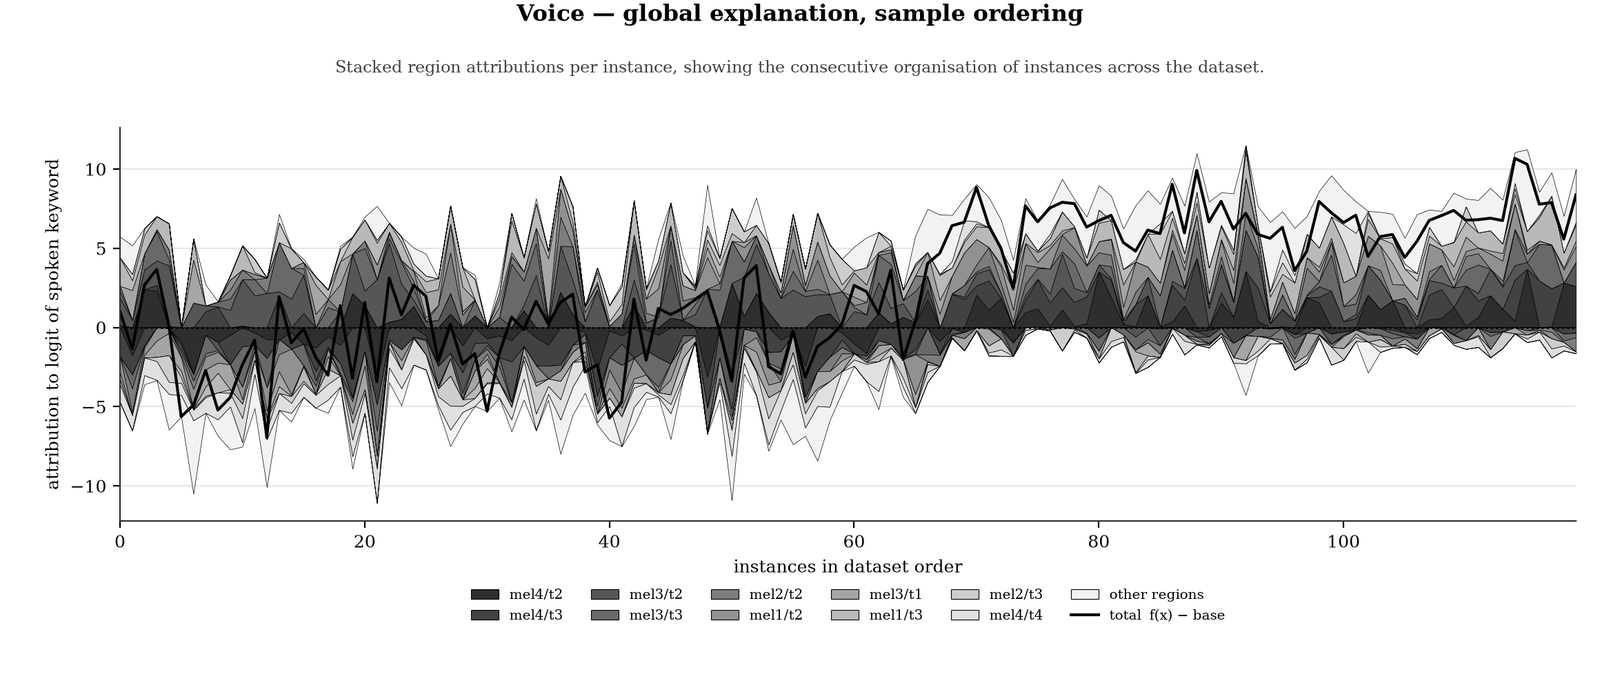
\includegraphics[width=\linewidth]{figures/attribution_voice_A4_ordering.png}
\caption{Voice --- global explanation under dataset ordering over the official test list.}
\label{fig:48}
\end{figure}

Explanations are stationary across the speaker-disjoint official test list, which is ordered independently of class and speaker, indicating speaker-invariant evidence regions: the network is not adapting its strategy to particular voices. Formally, regressing region attribution on test-list position yields no significant trend,

\begin{equation}
\label{eq:267}
| \;\text{corr}\;( \mathrm{Attr}(R_k ; x_{i}) , i ) | < \epsilon \;\text{for all k} ,
\end{equation}

which demonstrates mechanistically what the official split guarantees only by construction, and confirms that the 84.72 \% $\to$ 94.53 \% gain of \TABREF{11} reflects acoustic modelling rather than speaker-specific fitting --- the property a single-user assistive deployment depends on entirely.

\FloatBarrier

\subsection{Blink --- click generation}

Blink is the click, and it is the only modality with no pretrained neural comparison: as recorded in Section 4.2, the practical alternative is a geometric eye-aspect-ratio rule requiring full-face landmarks, which cannot be scored on 32 $\times$ 32 cropped eye regions, and no estimated figure is substituted in its place. Blink is therefore reported as a per-sample audit over 12,927 held-out eyes (4,453 open, 8,474 closed), which is the evidence required to set its operating threshold.

\TABREF{6} makes the framing unusually important here. A click is not one classification; it is a closure sustained past 420 ms --- $n_{\mathrm{run}}$ = 13 consecutive frames at 30 fps by \EQREF{120} --- with natural blinks of 100--300 ms rejected by construction. The governing quantity is therefore the integrity of a multi-frame run, not per-frame accuracy, and this section ends by showing that this \textbf{inverts} the cost asymmetry the raw confusion matrix suggests. Headline metrics, by \EQREF{140}--\EQREF{150}:

\begin{equation}
\label{eq:268}
\begin{aligned}
\mathrm{Acc} = 93.67 \% , \mathrm{BalAcc} = 93.32 \% , \\
\;\text{macro}\;-F_{1} = 93.04 \% ( 0.909 \;\text{open}, 0.951 \;\text{closed} ) ,
\end{aligned}
\end{equation}

\begin{equation}
\label{eq:269}
\begin{aligned}
\mathrm{MCC} = 0.8610 , \kappa = 0.8608 , \mathrm{ROC\text{-}AUC} = 0.9836 , \\
\mathrm{PR\text{-}AUC} = 0.9904 , \mathrm{Brier} = 0.0469 , \\
\mathrm{LogLoss} = 0.1700 ,
\end{aligned}
\end{equation}

with MCC as defined in \EQREF{144} \CITE{matthews} and $\kappa$ in \EQREF{145} \CITE{cohenkappa}.

\FIGREF{49} shows the raw score distribution.

\begin{figure}[pos=htbp]
\centering
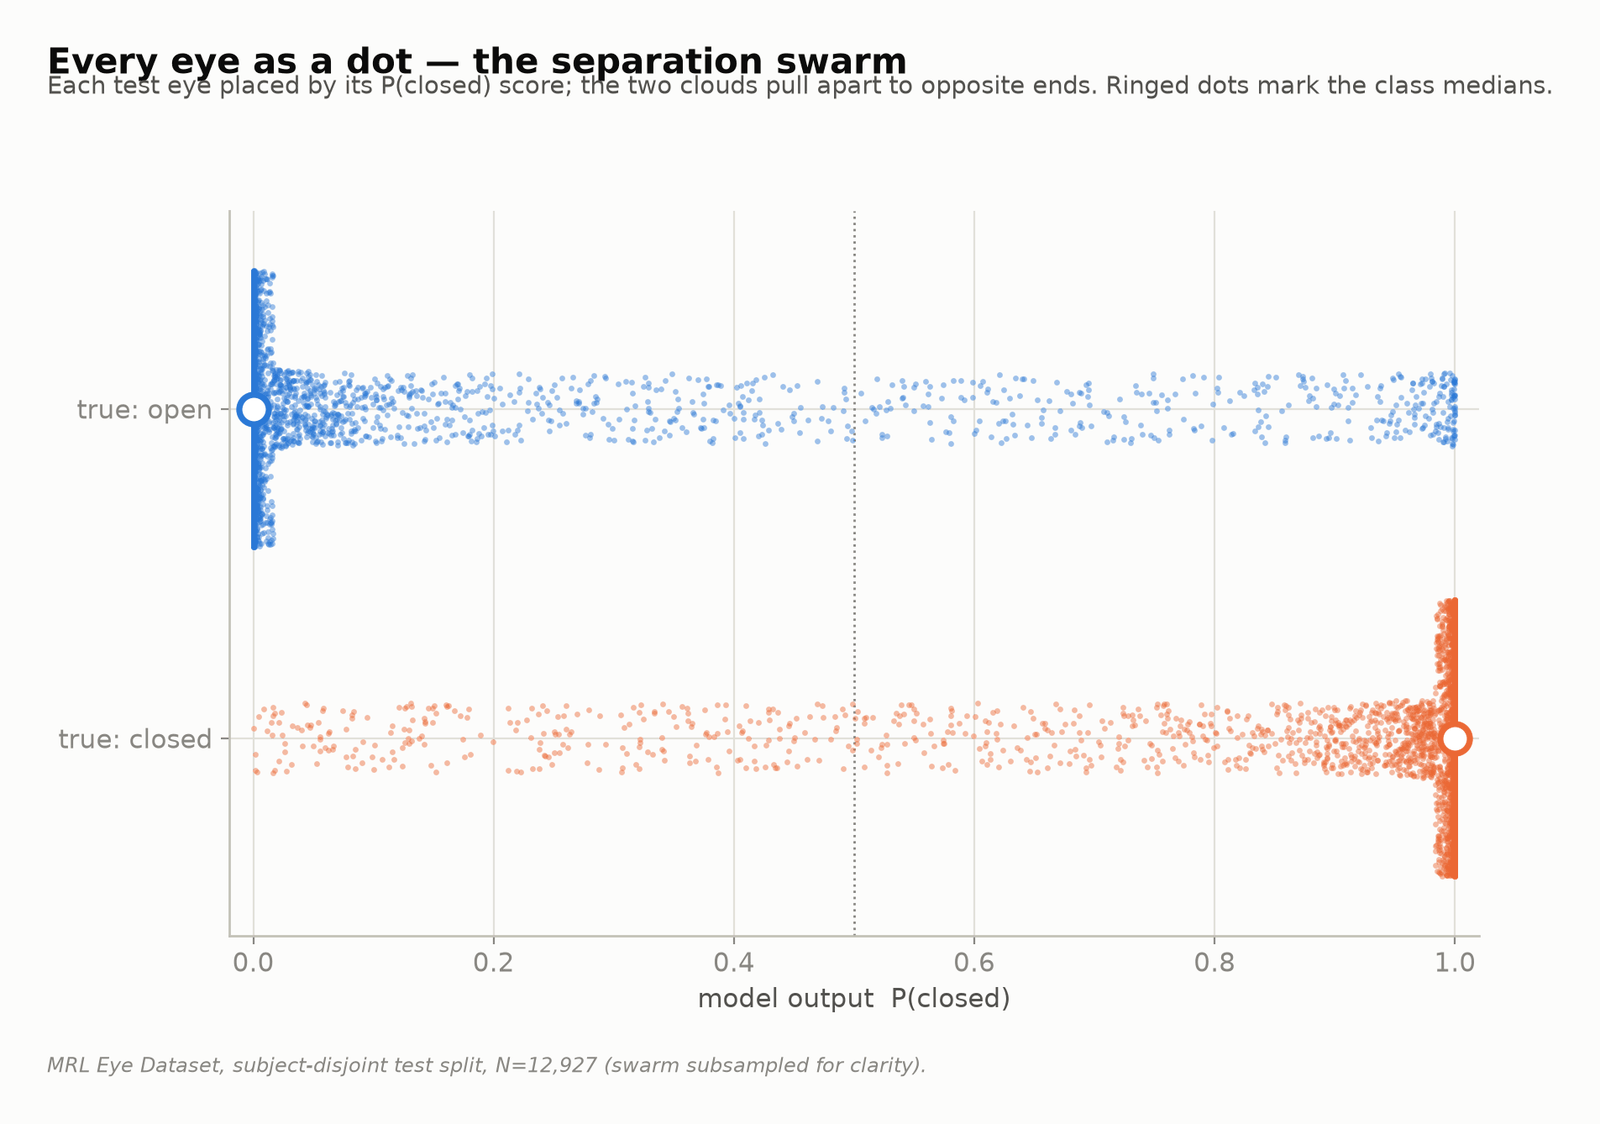
\includegraphics[width=\linewidth]{figures/blink_B1_swarm.png}
\caption{Separation swarm --- every test eye positioned by its predicted probability of the closed state.}
\label{fig:49}
\end{figure}

Two clouds occupy opposite extremes with a sparse interior, the visual form of 0.9836 ROC-AUC. The gap between ranking quality and operating-point accuracy is the actionable quantity:

\begin{equation}
\label{eq:270}
\mathrm{ROC\text{-}AUC} - \mathrm{Acc} = 0.9836 - 0.9367 = 0.0469 ,
\end{equation}

and a classifier ordering this well but scoring materially lower is \emph{misthresholded}, not underpowered. By the probabilistic identity \EQREF{146} the only samples that can change class under any threshold move are those in the overlap region, so the sparse interior also bounds what threshold tuning can recover --- which is why the threshold sweep of \FIGREF{52}, rather than a retraining effort, is the right next step.

\FIGREF{50} accounts for class prevalence.

\begin{figure}[pos=htbp]
\centering
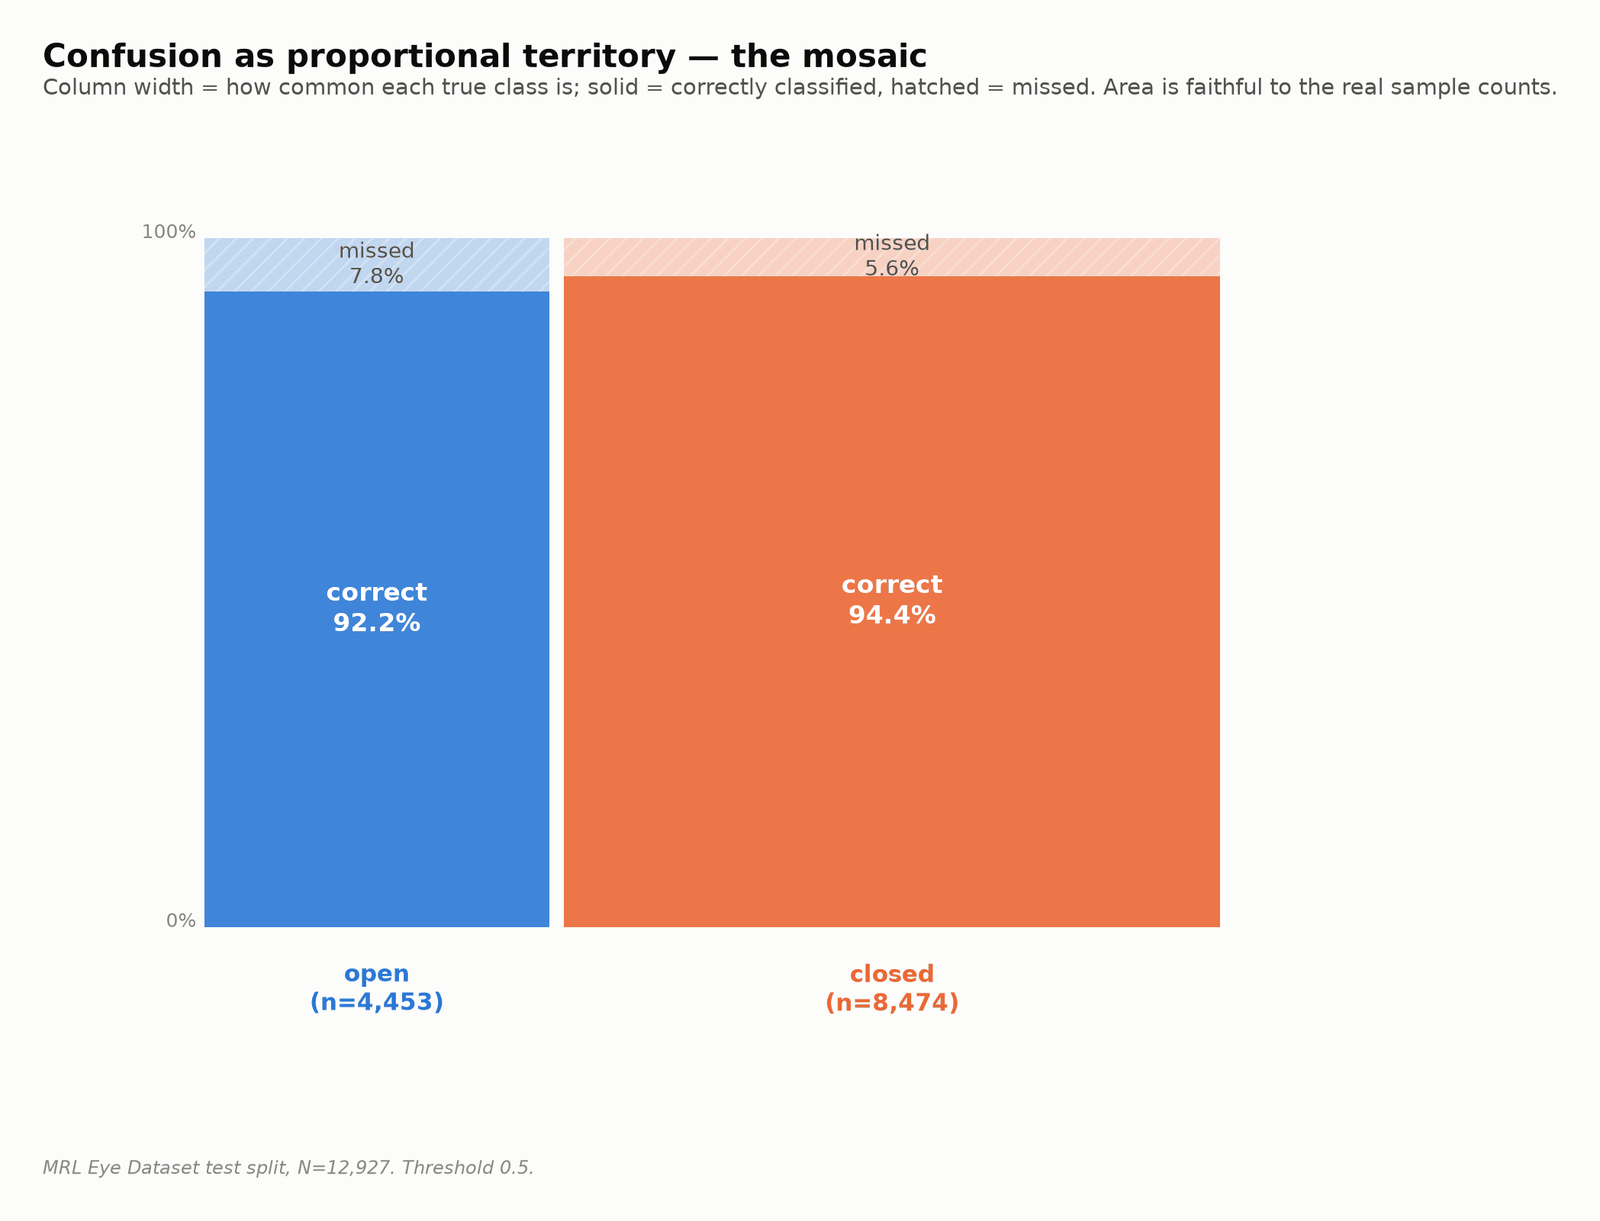
\includegraphics[width=\linewidth]{figures/blink_B2_mosaic.png}
\caption{Confusion mosaic --- territory proportional to class prevalence; column width is prior, solid area is correct classification.}
\label{fig:50}
\end{figure}

At 65.5 \% closed, accuracy is prevalence-weighted toward the majority class, so balanced accuracy \EQREF{141} and MCC \EQREF{144} are the appropriate summaries and both remain high; performance is therefore not a prior artefact. The mosaic exposes the asymmetry governing deployment:

\begin{equation}
\label{eq:271}
\begin{aligned}
\mathrm{FP} = 347 \;\text{open eyes classified closed}\; ( 7.79 \% \;\text{of open} ) , \\
\mathrm{FN} = 471 \;\text{closed eyes classified open}\; ( 5.56 \% \;\text{of closed} ) .
\end{aligned}
\end{equation}

At the frame level these are spurious-click and missed-blink pressure respectively; what the state machine of \ALGREF{5} makes of them is the subject of \FIGREF{52}.

\FIGREF{51} tests probabilistic honesty.

\begin{figure}[pos=htbp]
\centering
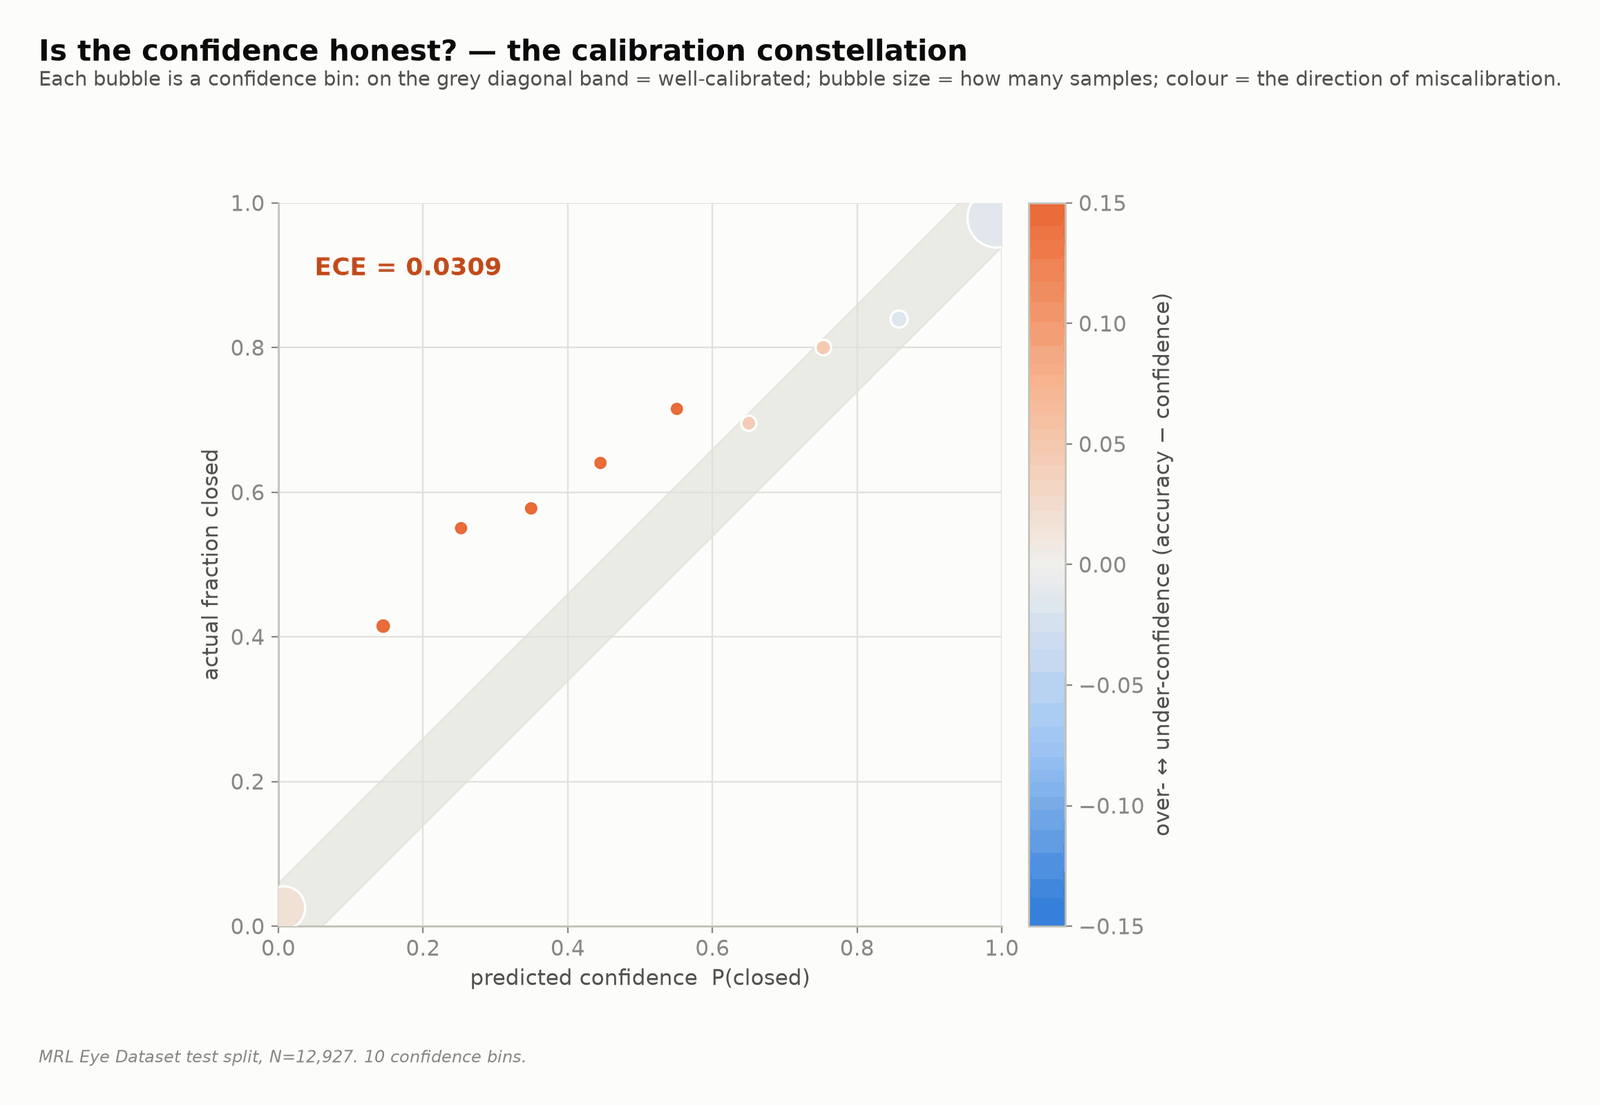
\includegraphics[width=\linewidth]{figures/blink_B3_constellation.png}
\caption{Calibration constellation --- confidence bins as bubbles against observed accuracy.}
\label{fig:51}
\end{figure}

Expected calibration error by \EQREF{150} is

\begin{equation}
\label{eq:272}
\begin{aligned}
\mathrm{ECE} = 2.48 \% , \mathbb{E}[ \text{conf}\; | \;\text{correct} ] = 0.973 , \\
\mathbb{E}[ \text{conf}\; | \;\text{error} ] = 0.785 ,
\end{aligned}
\end{equation}

consistent with the 0.0469 Brier score. The residual miscalibration exceeds the voice network's 1.54 \%, which is expected rather than anomalous: at 136,066 parameters on a binary task with a strong prior, the network sits in the regime where cross-entropy training drives logits toward saturation. Concretely, minimising \EQREF{88} on separable data drives $\|$f$\|$ $\to$ $\infty$ along the max-margin direction, and the induced posterior \EQREF{87} approaches a step function; the deviation from calibration is therefore a predictable consequence of the objective rather than a defect of the fit. Calibration nonetheless remains adequate for the state machine's staged progress readout (\ALGREF{5}, line 11), which reports fractional progress toward each click stage and therefore requires per-frame scores to be commensurable \emph{across} frames rather than merely correctly ordered \emph{within} one.

\FIGREF{52} sweeps the decision threshold --- the single most consequential deployment parameter for this modality.

\begin{figure}[pos=htbp]
\centering
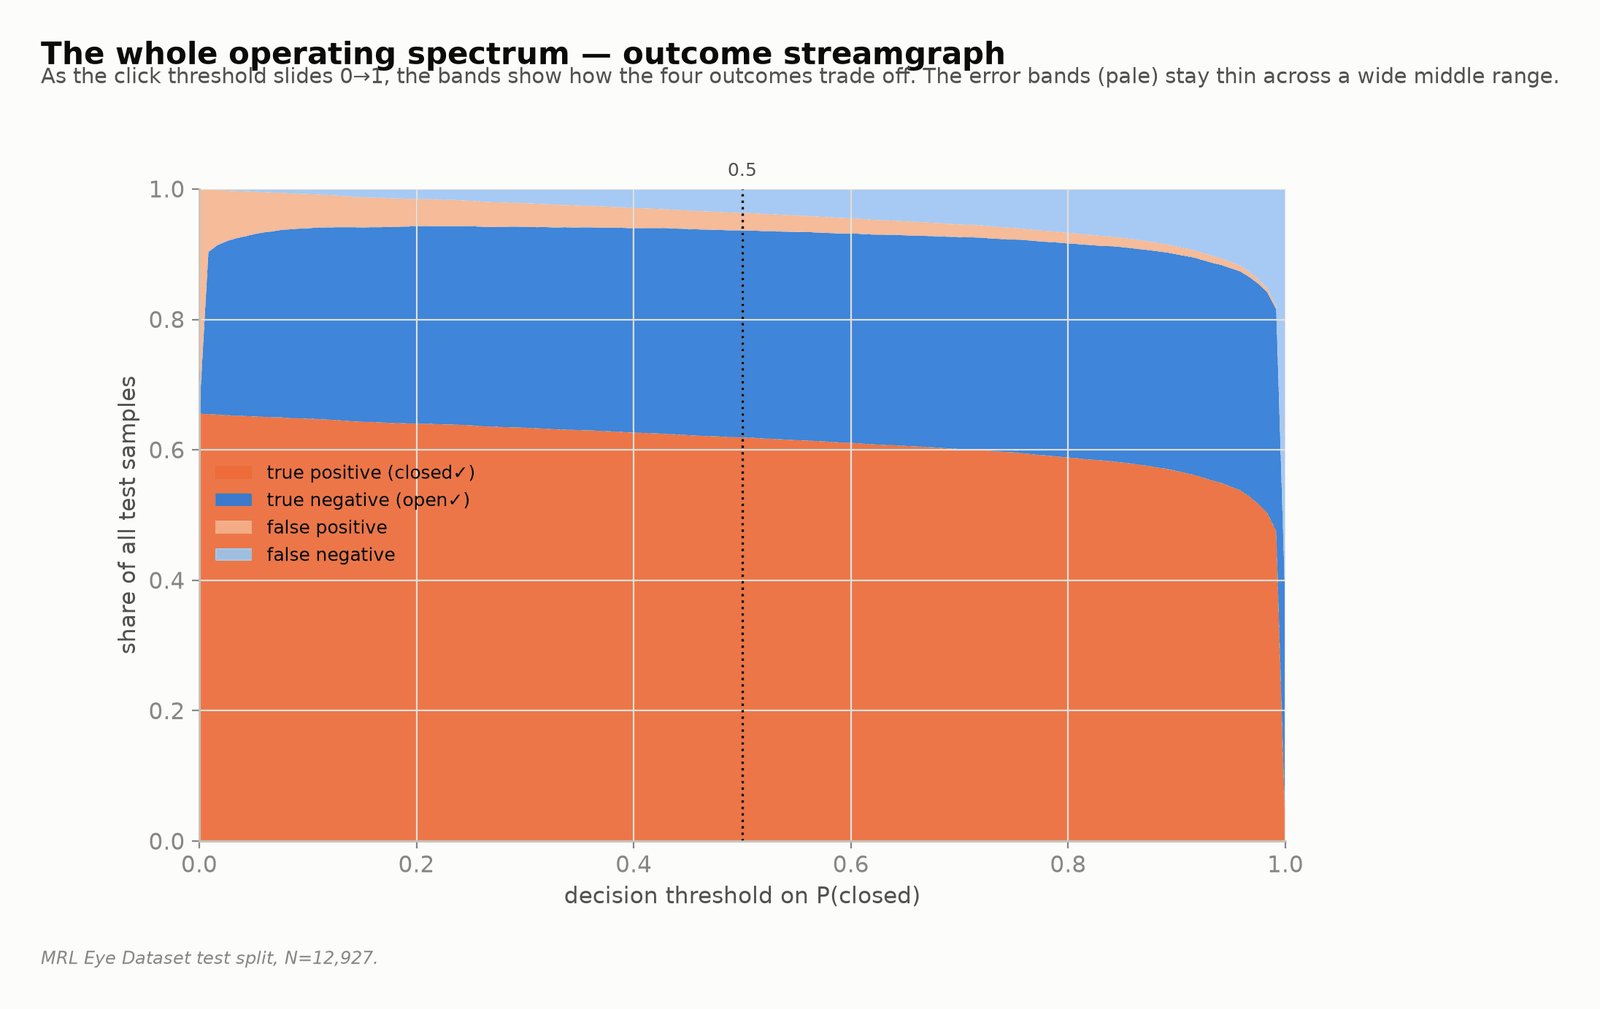
\includegraphics[width=\linewidth]{figures/blink_B4_streamgraph.png}
\caption{Outcome streamgraph --- the four confusion outcomes trading off continuously as the decision threshold slides from 0 to 1.}
\label{fig:52}
\end{figure}

The accuracy-optimal threshold is

\begin{equation}
\label{eq:273}
\begin{aligned}
\zeta _{\mathrm{acc}} = \mathrm{arg\,\mathrm{max}}_{\zeta} \mathrm{Acc}(\zeta ) = 0.212 , \\
\mathrm{Acc}(0.212) = 94.35 \% \mathrm{against} \mathrm{Acc}(0.50) = 93.67 \% ,
\end{aligned}
\end{equation}

and the Youden-optimal threshold \CITE{youden}, weighting both error types equally in rate terms, is

\begin{equation}
\label{eq:274}
\zeta _J = \mathrm{arg\,\mathrm{max}}_{\zeta} [ \mathrm{TPR}(\zeta ) - \mathrm{FPR}(\zeta ) ] = 0.426 .
\end{equation}

Minimising the cost-weighted objective

\begin{equation}
\label{eq:275}
C(\zeta ; w) = w \cdot \mathrm{FP}(\zeta ) + \mathrm{FN}(\zeta )
\end{equation}

for w $\in$ \{3, 5, 10\} gives $\zeta$* = 0.752, 0.845 and 0.955, cutting false positives from 347 to 226, 184 and 114 at the cost of 769, 955 and 1,492 missed blinks. The exchange is strongly non-linear:

\begin{equation}
\label{eq:276}
\Delta \mathrm{FN} / \Delta \mathrm{FP} : 298/121 = 2.46 \;\text{then}\; 186/42 = 4.43 ,
\end{equation}

so each successive false positive removed costs progressively more missed blinks --- the local slope of the receiver-operating curve steepening as the operating point moves into the tail.

\textbf{The cost-weighted reading is the natural one, and for this system it is wrong.} The reason is \EQREF{120}--\EQREF{123}. Because a click requires $n_{\mathrm{run}}$ = 13 consecutive frames above threshold, an isolated false positive cannot fire one; by \EQREF{121} the probability that noise alone manufactures a click from an open eye is

\begin{equation}
\label{eq:277}
\mathrm{FPR}^{n_{\mathrm{run}}} = 0.0779^{13} \approx 3.9 \times 10^{-15} ,
\end{equation}

and the state machine's duration requirement is therefore itself a powerful false-positive filter, with the 100--300 ms natural-blink rejection removing the most common sustained closure as well. A false \emph{negative}, by contrast, breaks a run in progress and silently cancels a click the user deliberately made; by \EQREF{122} the survival probability of a genuine run is

\begin{equation}
\label{eq:278}
( 1 - \mathrm{FNR} )^{n_{\mathrm{run}}} = 0.9444^{13} \approx 0.475 ,
\end{equation}

so under independence more than half of deliberate clicks would be lost. Under the deployed decision rule the asymmetry therefore \textbf{inverts} relative to the frame-level intuition, and thresholds \emph{below} 0.50 are the defensible choice: at $\zeta$ = 0.212 false negatives fall from 471 to 280, raising run survival to

\begin{equation}
\label{eq:279}
( 1 - 280/8474 )^{13} = 0.9670^{13} \approx 0.646 ,
\end{equation}

a 36 \% relative improvement in click retention, while spurious firing rises only to a still-negligible value by \EQREF{277}. The threshold $\zeta$ = 0.212 is thus simultaneously accuracy-optimal by \EQREF{273} and run-integrity-optimal by \EQREF{279}.

This conclusion depends on consecutive-frame errors being less than perfectly correlated. Under the Markov model \EQREF{123} with persistence $\varrho$ the effective run length is $n_{\mathrm{eff}}^{\mathrm{run}}$ = $n_{\mathrm{run}}$(1--$\varrho$)/(1+$\varrho$), and both \EQREF{277} and \EQREF{279} must be recomputed at $n_{\mathrm{eff}}^{\mathrm{run}}$; the \emph{direction} of the asymmetry is preserved for any $\varrho$ < 1, but its magnitude is not. That assumption is not tested here, and a live-session measurement of click precision and recall would be required to confirm it, which Section 6 records as an open item.

\FIGREF{53} shows the same structure as a flow.

\begin{figure}[pos=htbp]
\centering
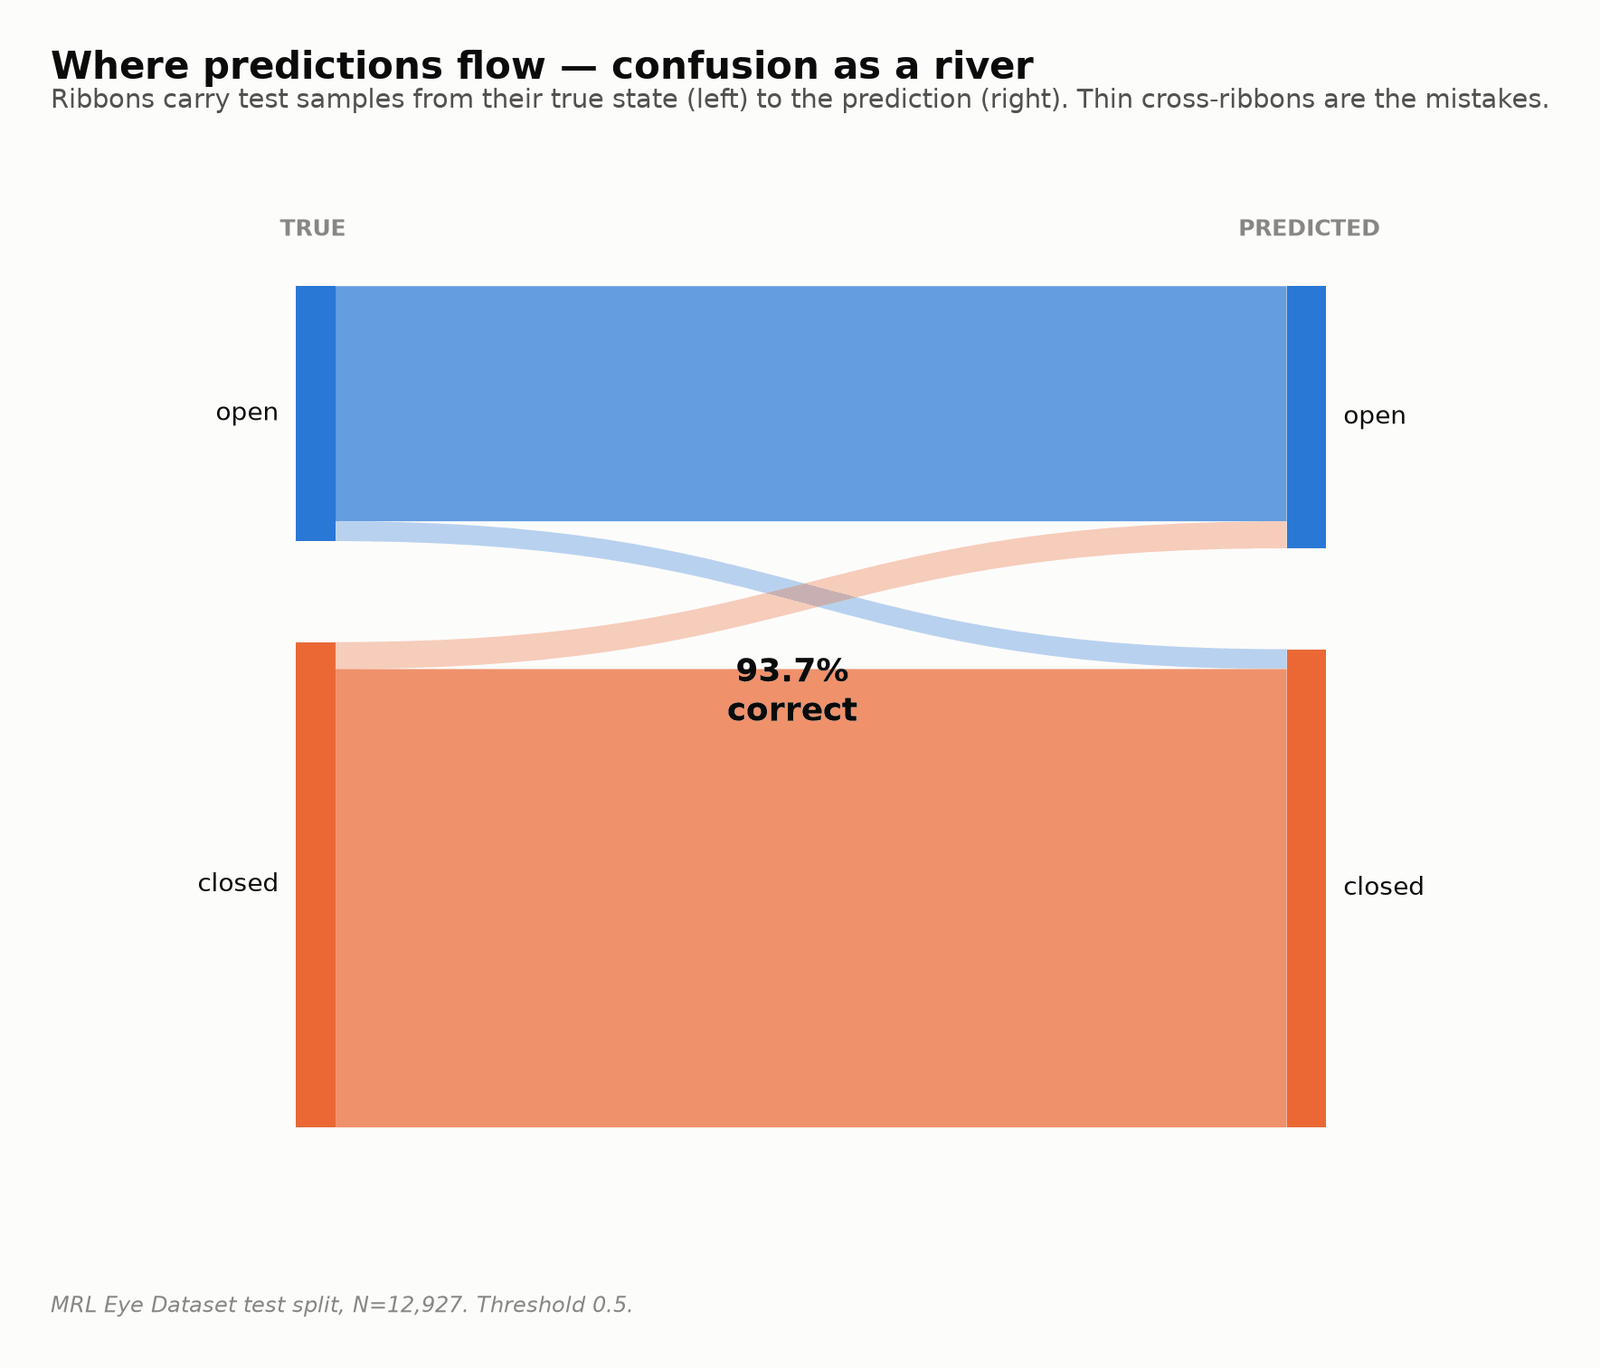
\includegraphics[width=\linewidth]{figures/blink_B5_confusion_flow.png}
\caption{Confusion as a river --- samples flowing from true to predicted state; cross-ribbons are errors.}
\label{fig:53}
\end{figure}

The two cross-ribbons are comparably thick (347 and 471) despite a 2:1 class imbalance, so per-class error \emph{rates} are asymmetric opposite to the prior:

\begin{equation}
\label{eq:280}
\mathrm{FPR} = 347/4453 = 7.79 \% \mathrm{against} \mathrm{FNR} = 471/8474 = 5.56 \% ,
\end{equation}

with per-class F$_{1}$ of 0.909 (open) against 0.951 (closed). This inverts the usual imbalance expectation --- the minority class is usually harder because it is scarcer --- and identifies \textbf{intra-class variance} rather than prior as the governing factor: the open class spans a wide appearance range (gaze direction, illumination, reflective eyewear) while the closed class is comparatively canonical. Formally, if the two classes have equal Bayes-optimal separability but unequal conditional entropy, then

\begin{equation}
\label{eq:281}
H( X | Y = \;\text{open} ) > H( X | Y = \;\text{closed} ) \implies \;\text{error rate}\;_{\mathrm{open}} > \;\text{error rate}\;_{\mathrm{closed}}
\end{equation}

at any fixed capacity. Rebalancing the training prior would therefore not help --- it addresses the wrong term --- whereas enlarging the open-class appearance range would, and eyewear is the specific variation the deployment gap of Section 6 names.

\FIGREF{54} measures score quality independently of any threshold.

\begin{figure}[pos=htbp]
\centering
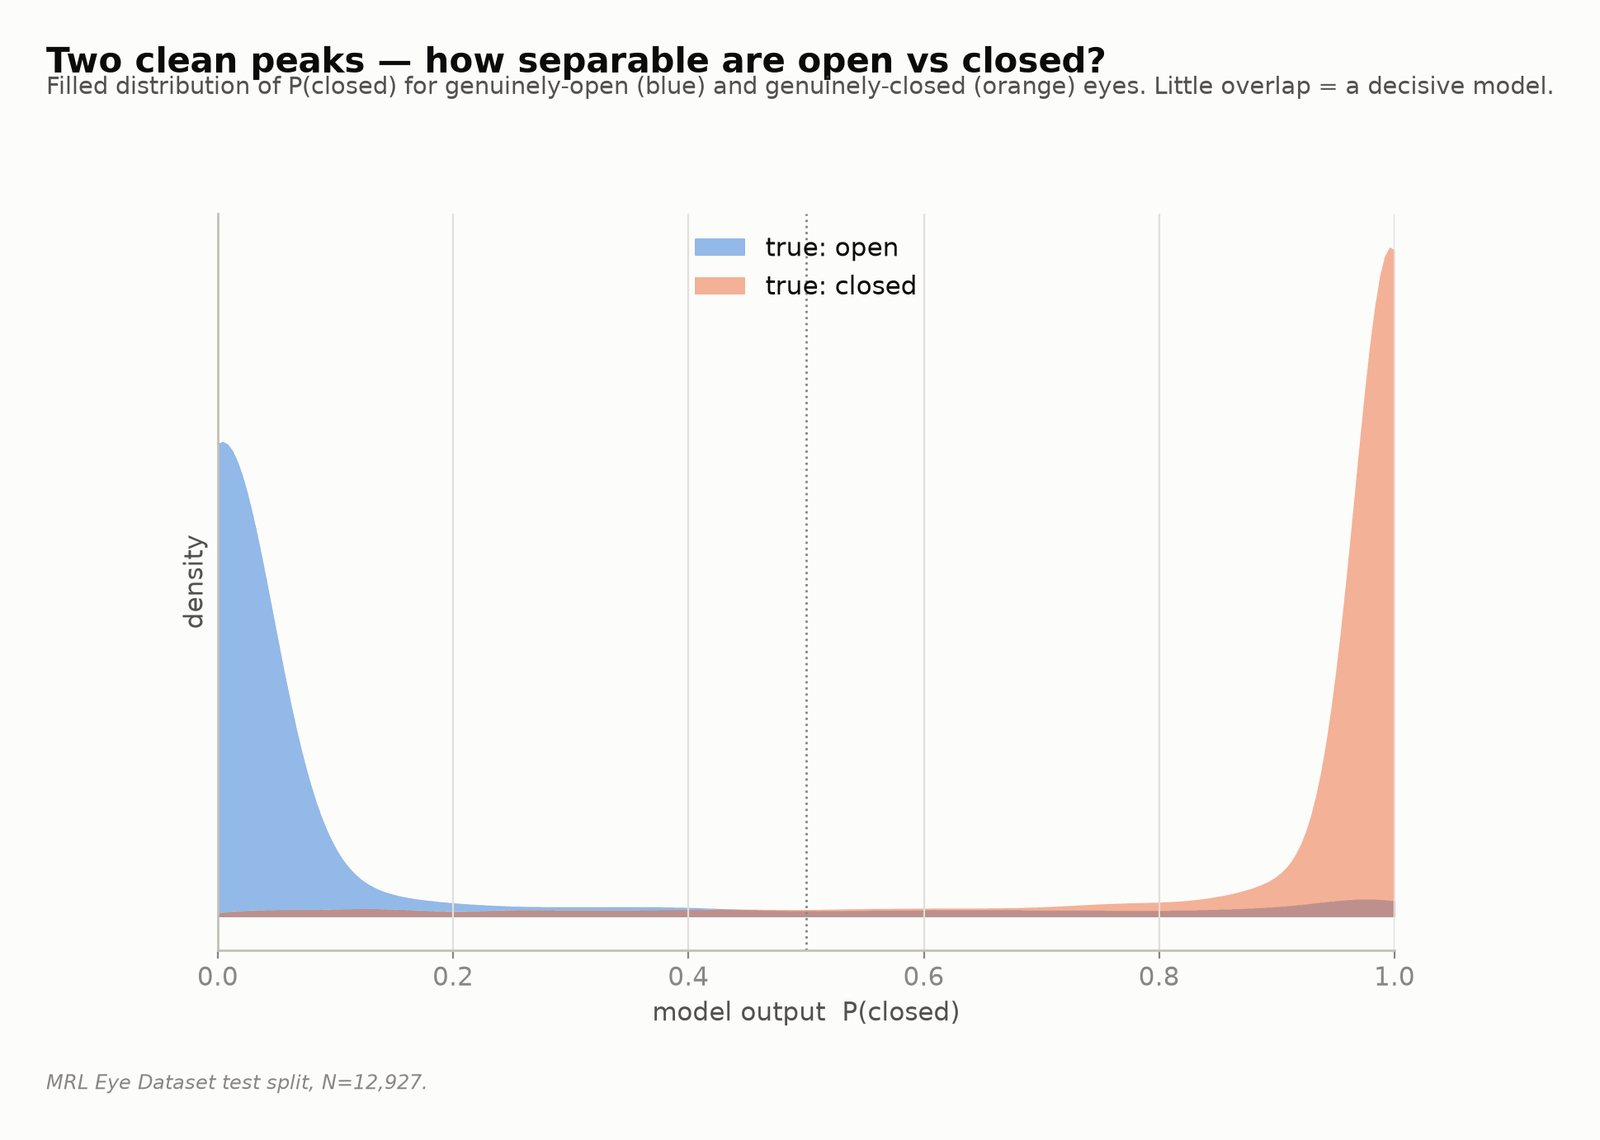
\includegraphics[width=\linewidth]{figures/blink_B6_score_separation.png}
\caption{Score separation --- how cleanly the predicted probability of the closed state divides the two classes.}
\label{fig:54}
\end{figure}

PR-AUC (0.9904) exceeding ROC-AUC (0.9836) is the expected relation on a majority-positive problem \CITE{davis}, since the precision axis is inflated by a high positive prior, and it confirms the ranking is robust under the operative class prior rather than only under a balanced one --- a distinction that matters because the deployed prior, dominated by open eyes during normal use, differs markedly from the test prior of 65.5 \% closed. Separation of this quality places the residual 6.33 \% error in genuinely ambiguous inputs: mid-blink frames where the eyelid is physically part-closed and the binary label is a quantisation of a continuous state. Writing the true eyelid aperture as a latent continuous variable a $\in$ [0,1] with the label y = $\mathbf{1}$[a < a$_{0}$], the conditional Bayes risk near the boundary is

\begin{equation}
\label{eq:282}
\mathbb{P}[ \text{error}\; | a \approx a_{0} ] \to \tfrac{1}{2} ,
\end{equation}

irreducibly, so that component of the error cannot be removed at the per-frame level by any classifier. This is precisely the argument for resolving it temporally, which is what the duration requirement of \EQREF{118} does.

\FIGREF{55} tests whether the network signals its own errors.

\begin{figure}[pos=htbp]
\centering
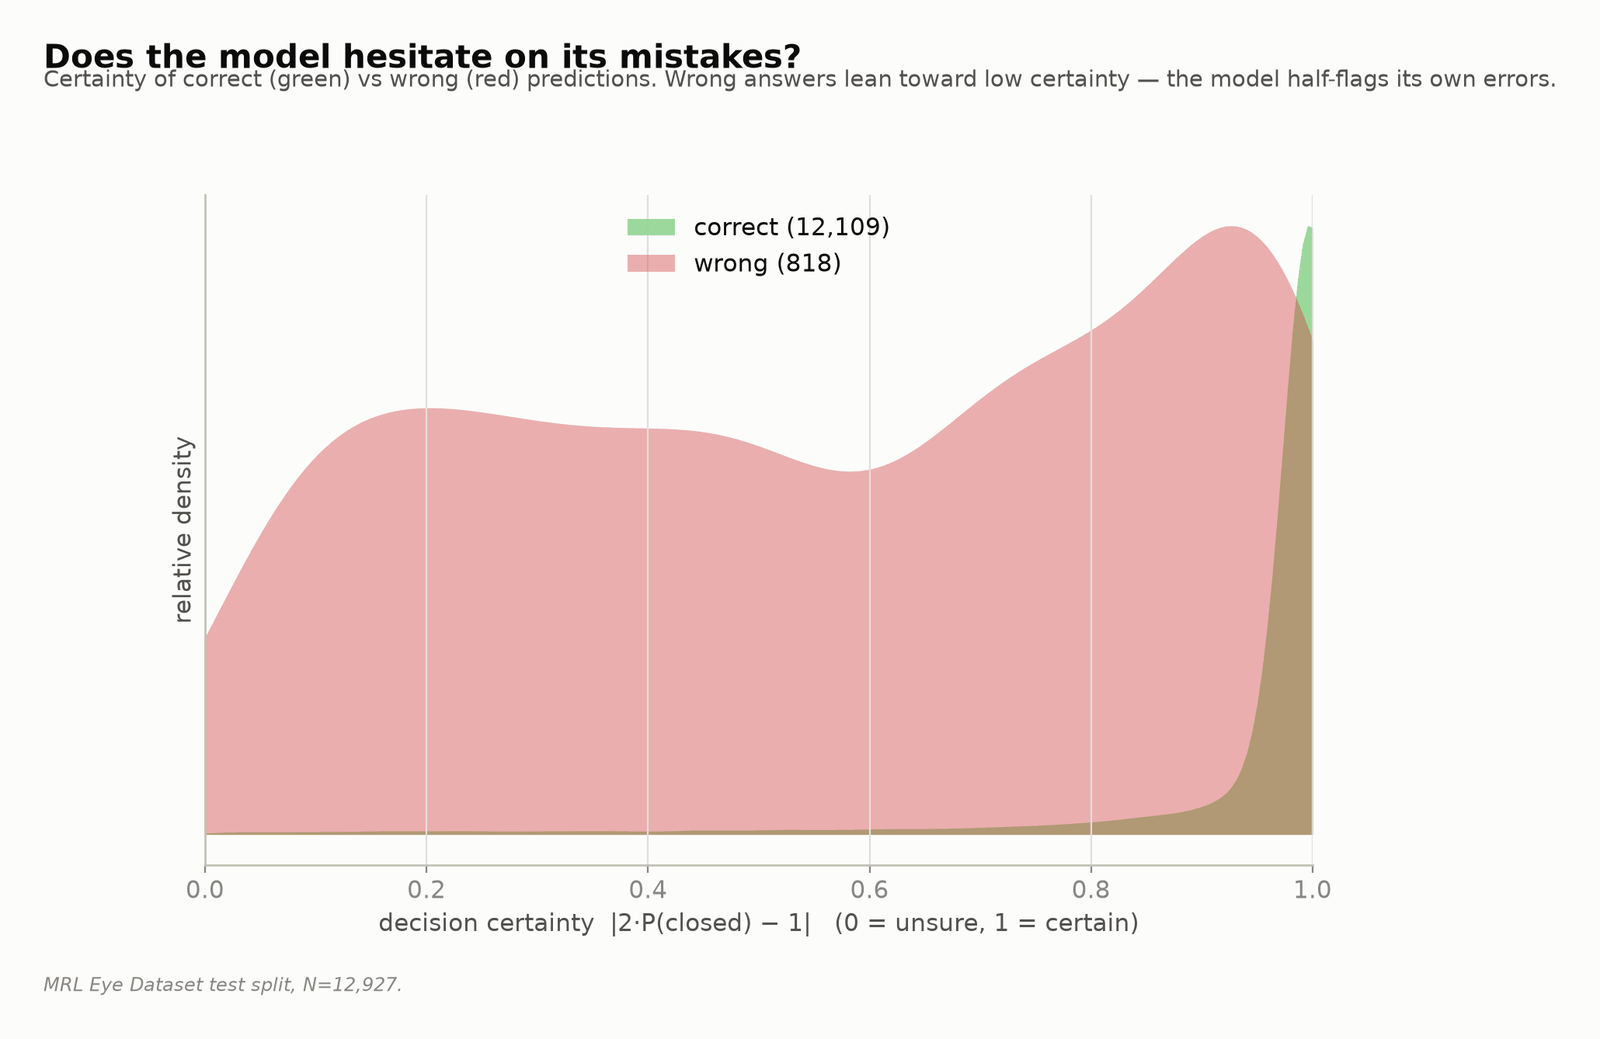
\includegraphics[width=\linewidth]{figures/blink_B7_margin_ridge.png}
\caption{Decision certainty --- the certainty distribution of correct against incorrect predictions.}
\label{fig:55}
\end{figure}

Confidence is a strong but incomplete error detector, AUC 0.9148, and the quintile profile makes the limitation precise. Error rates across confidence quintiles run

\begin{equation}
\label{eq:283}
26.60 \% , 3.95 \% , 0.85 \% , 0.19 \% , 0.04 \% ,
\end{equation}

a spread of

\begin{equation}
\label{eq:284}
26.60 / 0.04 = 665\times
\end{equation}

from lowest to highest. Yet

\begin{equation}
\label{eq:285}
\mathbb{P}[ \text{conf}\; > 0.9 | \;\text{error} ] = 31.2 \% ,
\end{equation}

so roughly one error in three is \emph{confidently wrong} and unreachable by any per-frame gate. This is the quantitative justification for the state machine's duration requirement rather than a confidence threshold: mid-blink ambiguity in the sense of \EQREF{282} is transient while a genuine closure persists, so consecutive-frame agreement suppresses exactly the confident isolated errors that per-frame confidence cannot. Formally, a per-frame gate at level $\zeta_{c}$ reduces error by at most 1 -- $\mathbb{P}$[conf > $\zeta_{c}$ | error], bounded below by 0.312 here, whereas the run requirement suppresses isolated errors at rate governed by \EQREF{277} irrespective of their confidence.

\FIGRANGE{56}{59} re-render the same scores, testing the locality of misordering and the shape of the threshold trade.

\begin{figure}[pos=htbp]
\centering
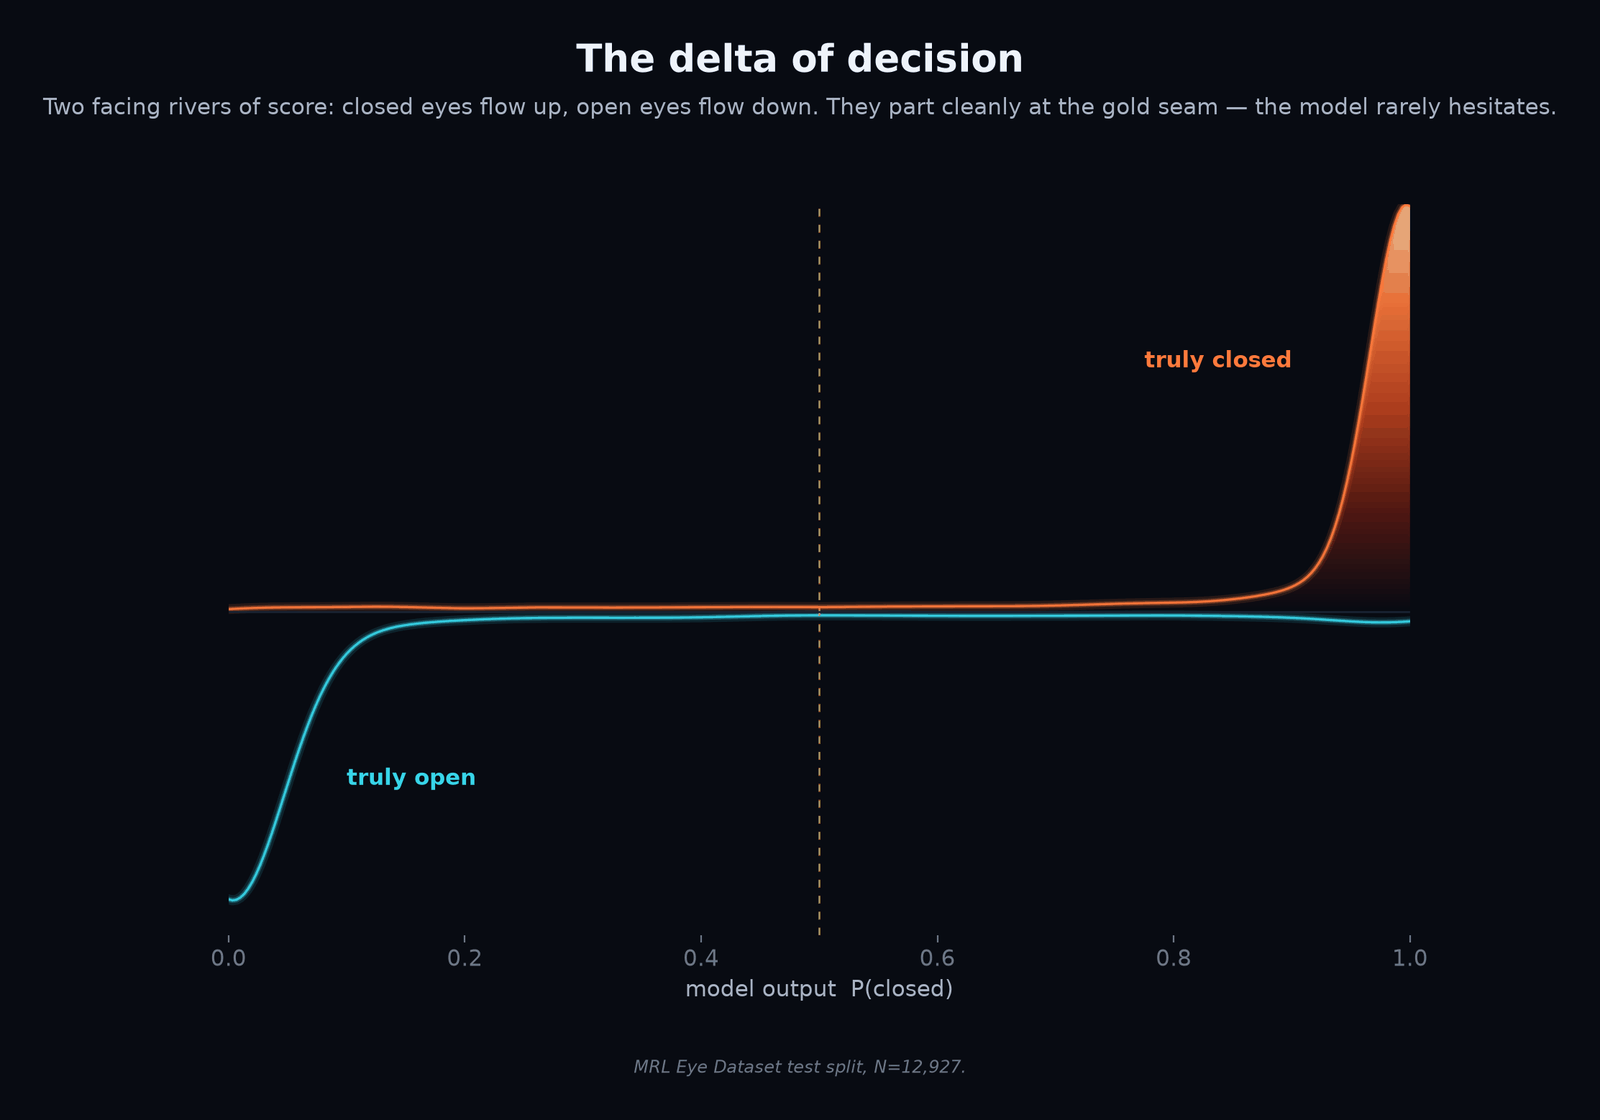
\includegraphics[width=\linewidth]{figures/figures_art_blink_BA1_delta_stream.png}
\caption{The delta of decision --- two facing rivers of predicted score, closed eyes flowing upward and open eyes downward, parting at the decision threshold.}
\label{fig:56}
\end{figure}

The rivers are near-disjoint except at a narrow waist, the geometric expression of 0.9836 ROC-AUC and 0.9904 PR-AUC, and all 6.33 \% of the error lives in that waist --- which is why threshold placement rather than representation is the operative parameter. The asymmetry about the parting line previews the cost analysis: the closed-eye river is the larger (8,474 against 4,453), so shifting the threshold to suppress false clicks sacrifices a disproportionate number of closed-eye detections, which is the non-linear exchange rate measured in \EQREF{276}.

\begin{figure}[pos=htbp]
\centering
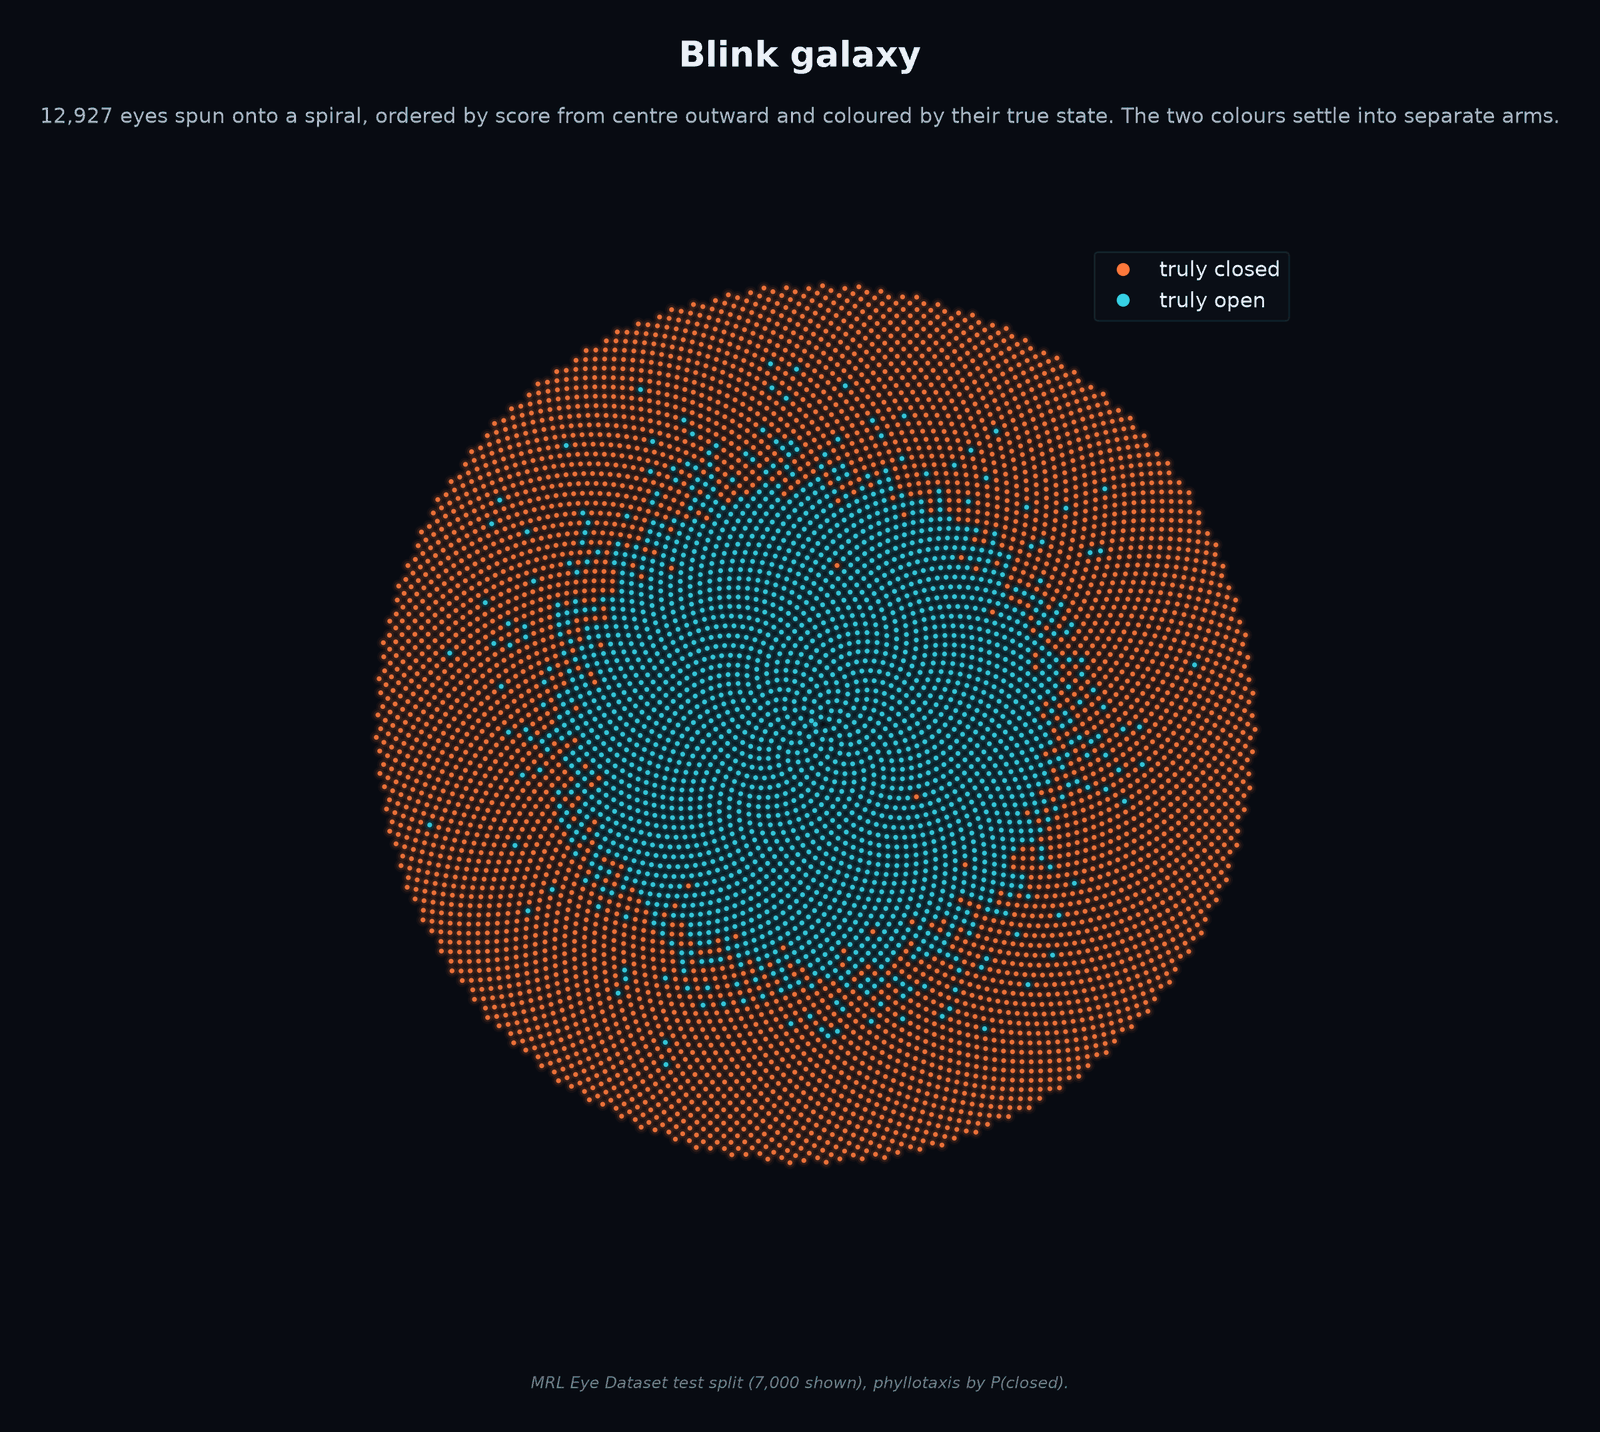
\includegraphics[width=\linewidth]{figures/figures_art_blink_BA2_galaxy.png}
\caption{Blink galaxy --- all 12,927 test eyes arranged on a spiral in order of predicted score and coloured by their true state.}
\label{fig:57}
\end{figure}

Ordering by score and colouring by truth renders ranking quality \emph{countable}. By the identity \EQREF{146}, ROC-AUC is exactly the probability that a randomly chosen closed eye outranks a randomly chosen open one, so contaminated arc length relative to the whole spiral is a direct visual estimate of

\begin{equation}
\label{eq:286}
1 - \mathrm{AUC} = 0.0164 .
\end{equation}

Contamination is confined to a short arc at the crossover rather than distributed along the spiral, establishing that misordering is \textbf{local} --- the precondition for threshold tuning to be effective at all, and therefore the justification for treating \FIGREF{52} as the primary improvement lever. Had misordering been distributed, no threshold would recover the gap \EQREF{270} and retraining would be the only route.

\begin{figure}[pos=htbp]
\centering
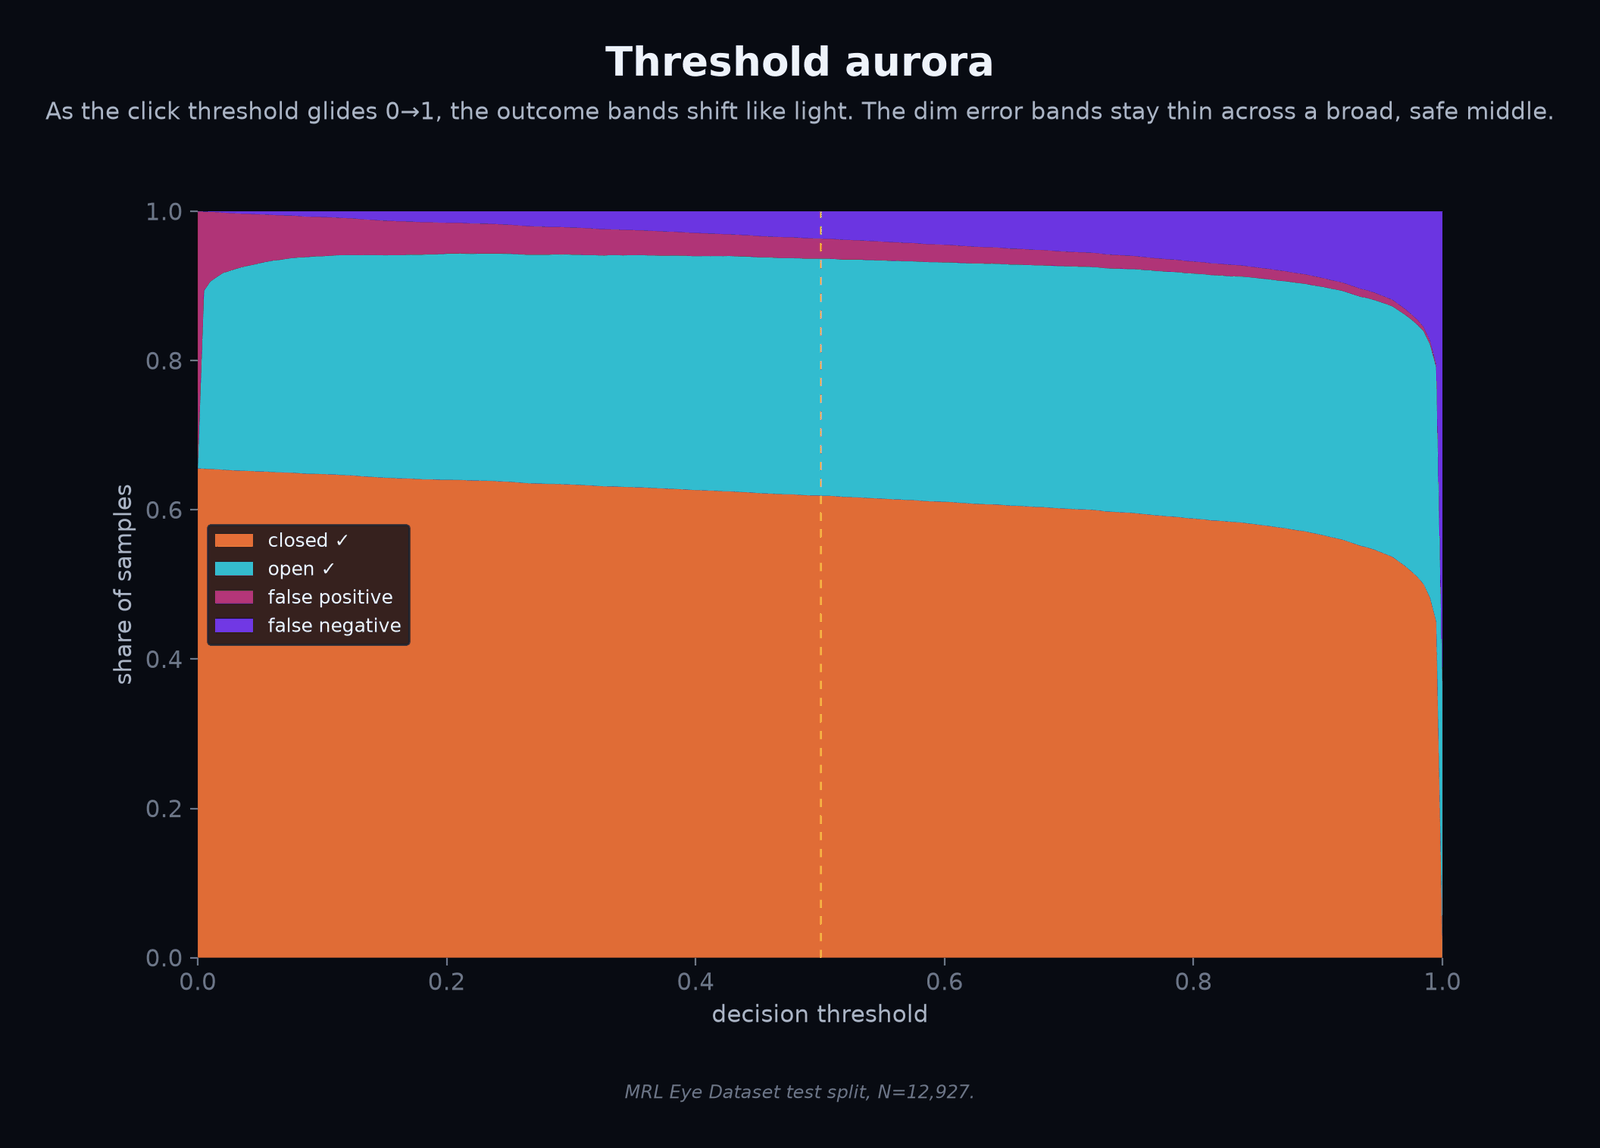
\includegraphics[width=\linewidth]{figures/figures_art_blink_BA3_threshold_aurora.png}
\caption{Threshold aurora --- the four confusion outcomes as continuous bands, as the decision threshold glides from 0 to 1.}
\label{fig:58}
\end{figure}

Continuous rendering exposes gradients the sampled points of \FIGREF{52} cannot. Accuracy peaks at 94.35 \% near $\zeta$ = 0.212 and declines to 93.67 \% at 0.50 while the false-positive band contracts monotonically throughout, so

\begin{equation}
\label{eq:287}
\text{dAcc}\;/d\zeta < 0 \;\text{and dFP}\;/d\zeta < 0 \;\text{simultaneously on}\; \zeta \in [0.212, 1] ,
\end{equation}

meaning the two objectives move in opposite directions with no crossing point and \textbf{no threshold is jointly optimal}. The cost-weighted optima of \EQREF{275} are then read directly off the band gradients. The figure converts an implicit design assumption --- how much worse is a false click than a missed blink --- into an explicit tunable with a measured response curve, which is what allows the conclusion of \EQREF{277}--\EQREF{279} to be revised once the state machine is taken into account rather than argued in the abstract.

\begin{figure}[pos=htbp]
\centering
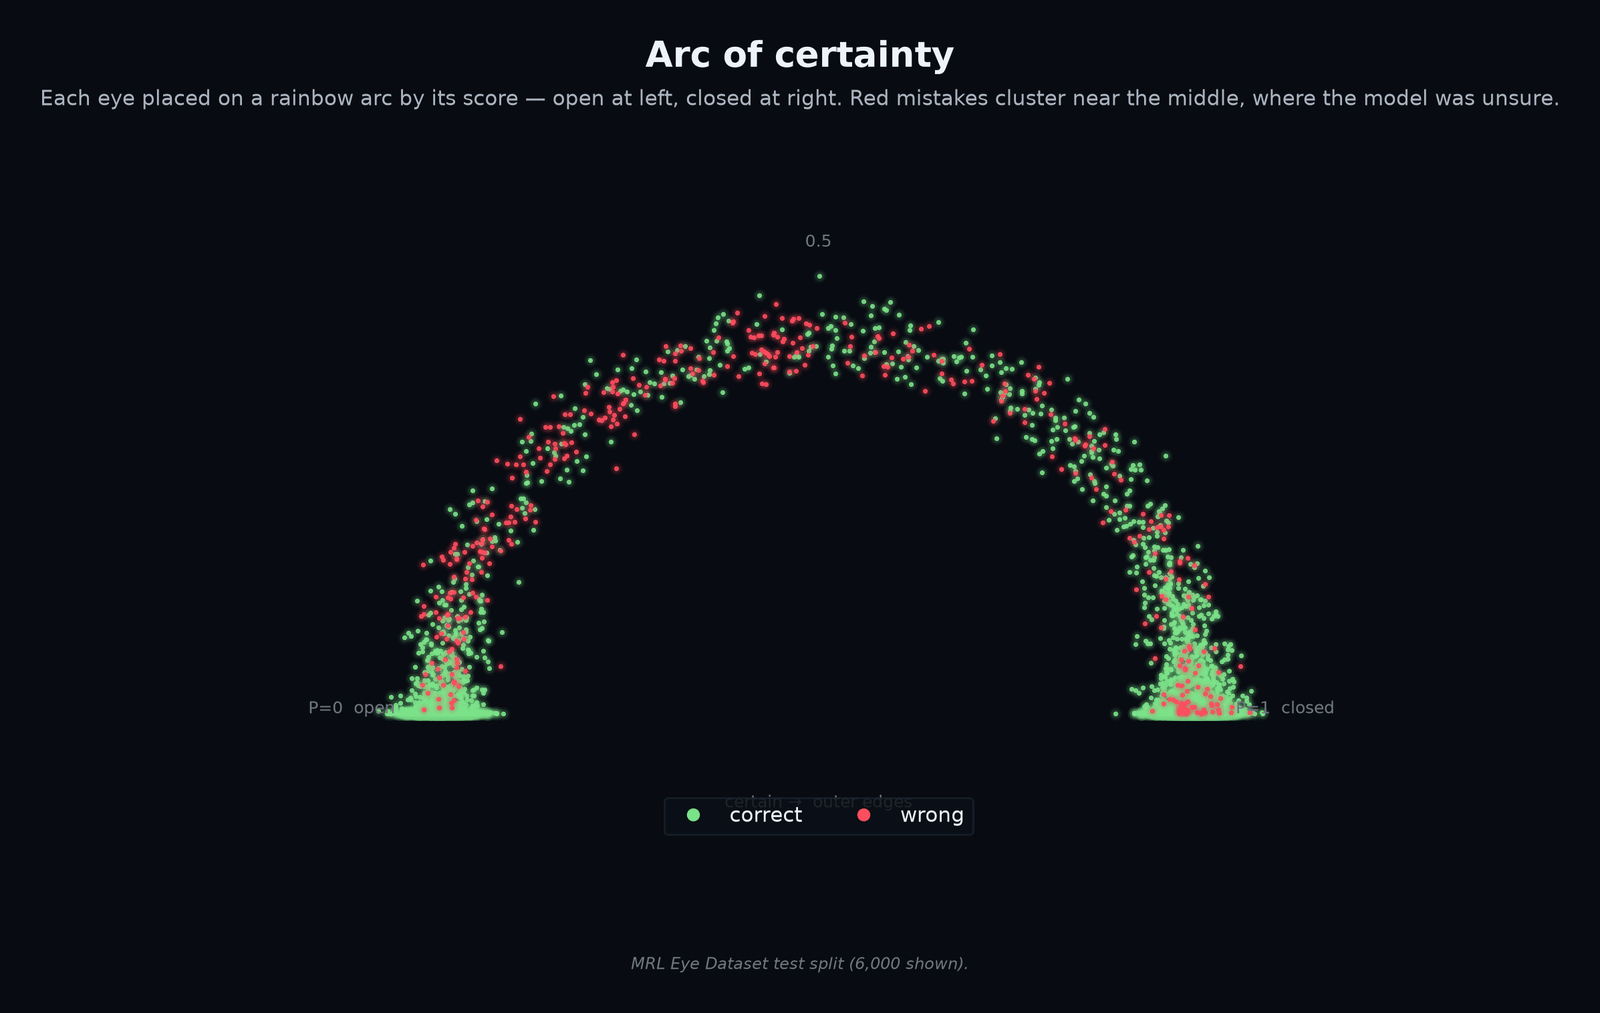
\includegraphics[width=\linewidth]{figures/figures_art_blink_BA4_certainty_arc.png}
\caption{Arc of certainty --- every test eye positioned along an arc by its predicted score, with errors highlighted.}
\label{fig:59}
\end{figure}

Errors concentrate near the arc's centre where certainty is lowest, the basis for uncertainty-aware gating, with error rates falling across quintiles by \EQREF{283}. The counter-population limits the approach: by \EQREF{285}, 31.2 \% of errors sit at the extremes where no gate reaches them. Per-frame uncertainty filtering therefore has a hard floor, and the deployed state machine aggregates across consecutive frames precisely because temporal persistence discriminates where per-frame certainty cannot.

\subsubsection{Why this modality generalises across subjects}

\begin{figure}[pos=htbp]
\centering
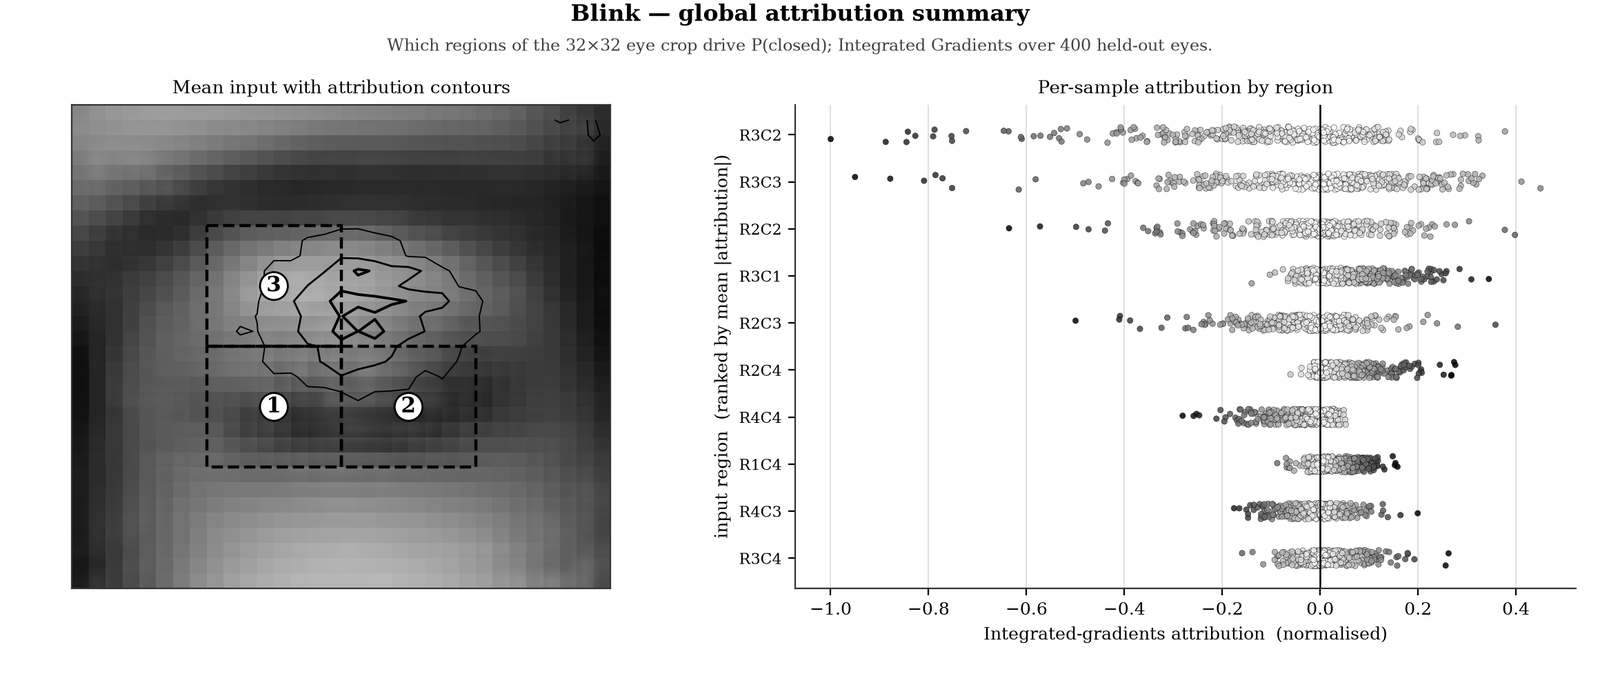
\includegraphics[width=\linewidth]{figures/attribution_blink_A1_summary.png}
\caption{Blink --- global attribution summary: regions of the 32 $\times$ 32 eye crop ranked by mean absolute attribution, with per-sample distributions and the three strongest regions outlined on the mean input.}
\label{fig:60}
\end{figure}

Attribution concentrates in R3C2, R3C3 and R2C2 --- the central and lower-central band containing the palpebral fissure --- while the four corner regions contribute near-zero attribution with tightly clustered per-sample distributions:

\begin{equation}
\label{eq:288}
\begin{aligned}
\Sigma _{k \in \;\text{centre}} | \mathrm{Attr}(R_k) | / \Sigma _k | \mathrm{Attr}(R_k) | \\ 
\gg \\ 
\Sigma _{k \in \;\text{corners}} | \mathrm{Attr}(R_k) | / \Sigma _k | \mathrm{Attr}(R_k) | .
\end{aligned}
\end{equation}

The network located the anatomically correct evidence region without spatial supervision and, more importantly, learned to \emph{ignore} the periphery where hair, spectacle frames and background offer identity-correlated shortcuts. This is the mechanistic basis of its cross-subject robustness: a detector attending only to the fissure is structurally invariant to the appearance factors the leaked-partition evaluation of Section 5.1.1 was silently exploiting. Formally, if the attribution mass on identity-correlated regions is negligible, then the decision function is approximately measurable with respect to the fissure sub-$\sigma$-algebra, and identity enters only through it.

\begin{figure}[pos=htbp]
\centering
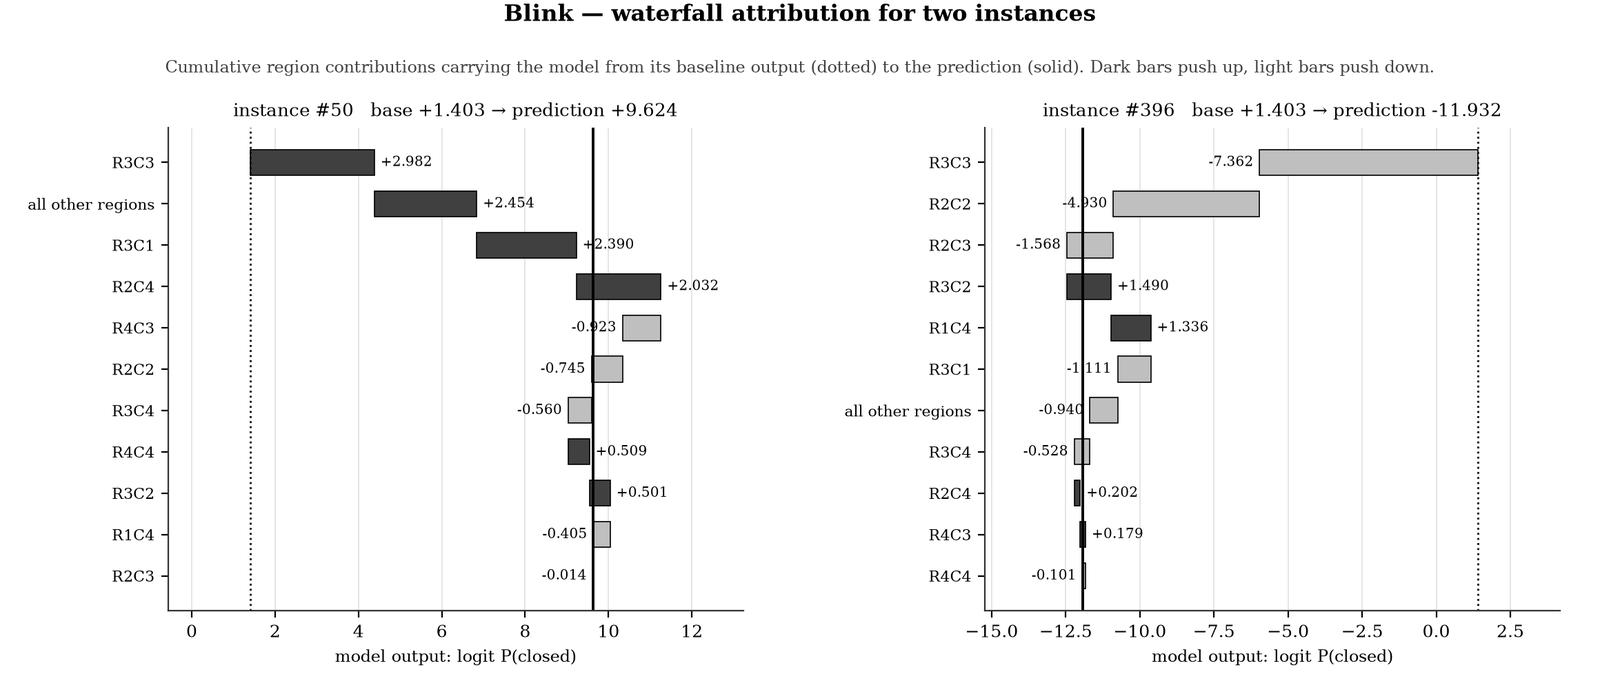
\includegraphics[width=\linewidth]{figures/attribution_blink_A2_waterfall.png}
\caption{Blink --- waterfall attribution for the two most extreme instances, carrying the network from baseline output to prediction region by region.}
\label{fig:61}
\end{figure}

Completeness \EQREF{138} makes this an audit rather than an illustration: the bars sum to the full logit displacement F(x) -- F(0). For both extremes two or three central regions dominate, the remaining thirteen contributing a small alternating-sign residual, so the decision is effectively low-dimensional in region space:

\begin{equation}
\label{eq:289}
\text{effective dimension}\; \approx | { k : |\mathrm{Attr}(R_k)| > 0.1 \cdot \mathrm{max}_j |\mathrm{Attr}(R_j)| } | \approx 3 of 16 .
\end{equation}

This is why 136,066 parameters suffice and why inference costs 0.42 ms --- the capacity requirement is set by the intrinsic dimensionality of the evidence, not by the input dimension, and that is what leaves frame budget for the other three modalities under \EQREF{165}.

\begin{figure}[pos=htbp]
\centering
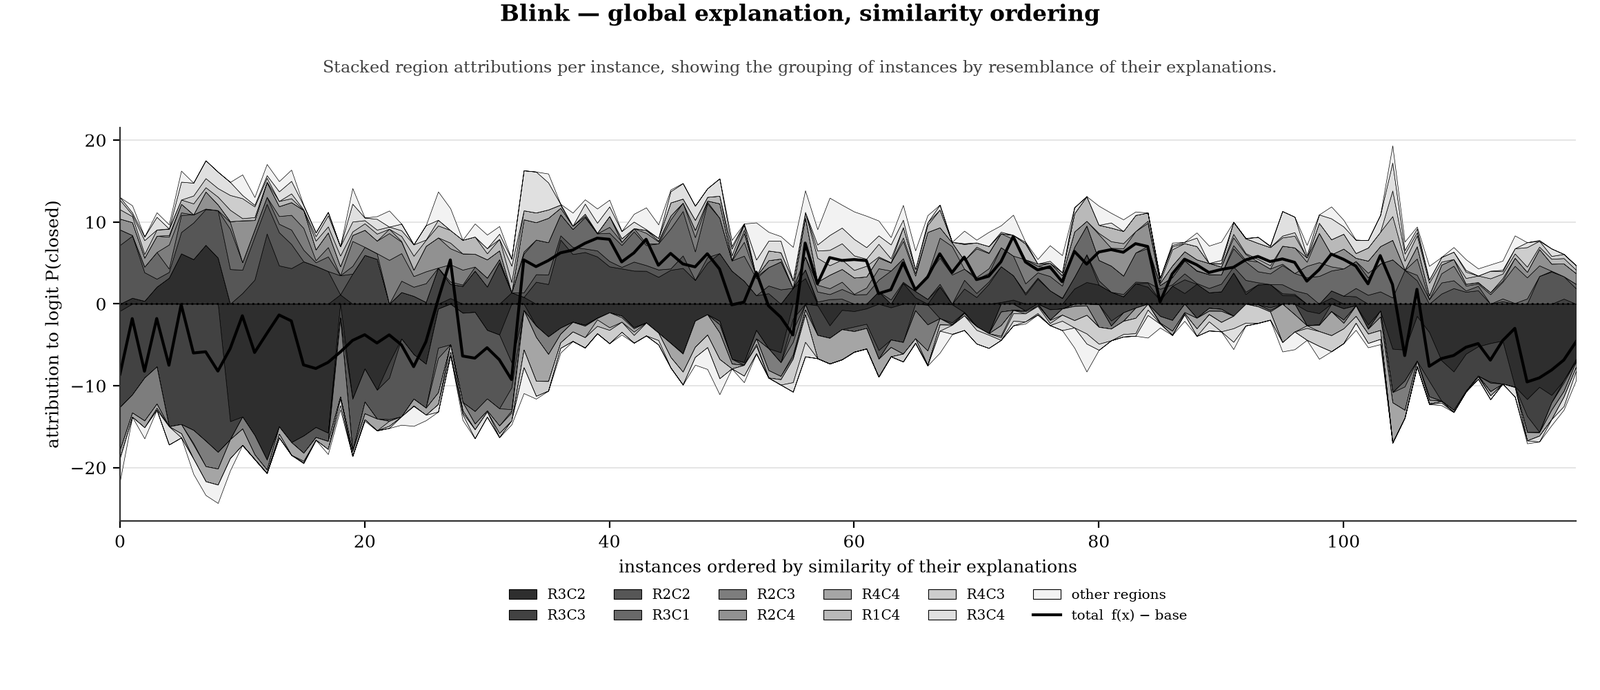
\includegraphics[width=\linewidth]{figures/attribution_blink_A3_similarity.png}
\caption{Blink --- global explanation under similarity ordering: stacked region attributions with instances ordered by resemblance of their explanations.}
\label{fig:62}
\end{figure}

Similarity ordering yields contiguous \textbf{blocks} rather than a gradient, indicating a small number of discrete strategies rather than one continuously varying rule --- the categorical-task structure also seen for voice in \FIGREF{47}, and the opposite of the continua of gaze and head pose. The blocks align with the two classes and, within them, with the \emph{sign pattern} of the central regions, which is evidence that eye state is encoded through the polarity of a localised contrast measurement rather than a distributed template:

\begin{equation}
\label{eq:290}
F_{\mathrm{blink}}(x) \approx w \cdot \mathrm{sgn}( \langle x, \phi _{\mathrm{upper}} \rangle - \langle x, \phi _{\mathrm{lower}} \rangle ) ,
\end{equation}

approximately. A polarity code is cheap to compute and inherently robust to global illumination scaling, since a multiplicative photometric change leaves the sign of a difference unaltered --- consistent with the normalisation \EQREF{15}, with stability across the illumination range present in the corpus, and with the modality's tolerance of the variable lighting a home deployment presents.

\begin{figure}[pos=htbp]
\centering
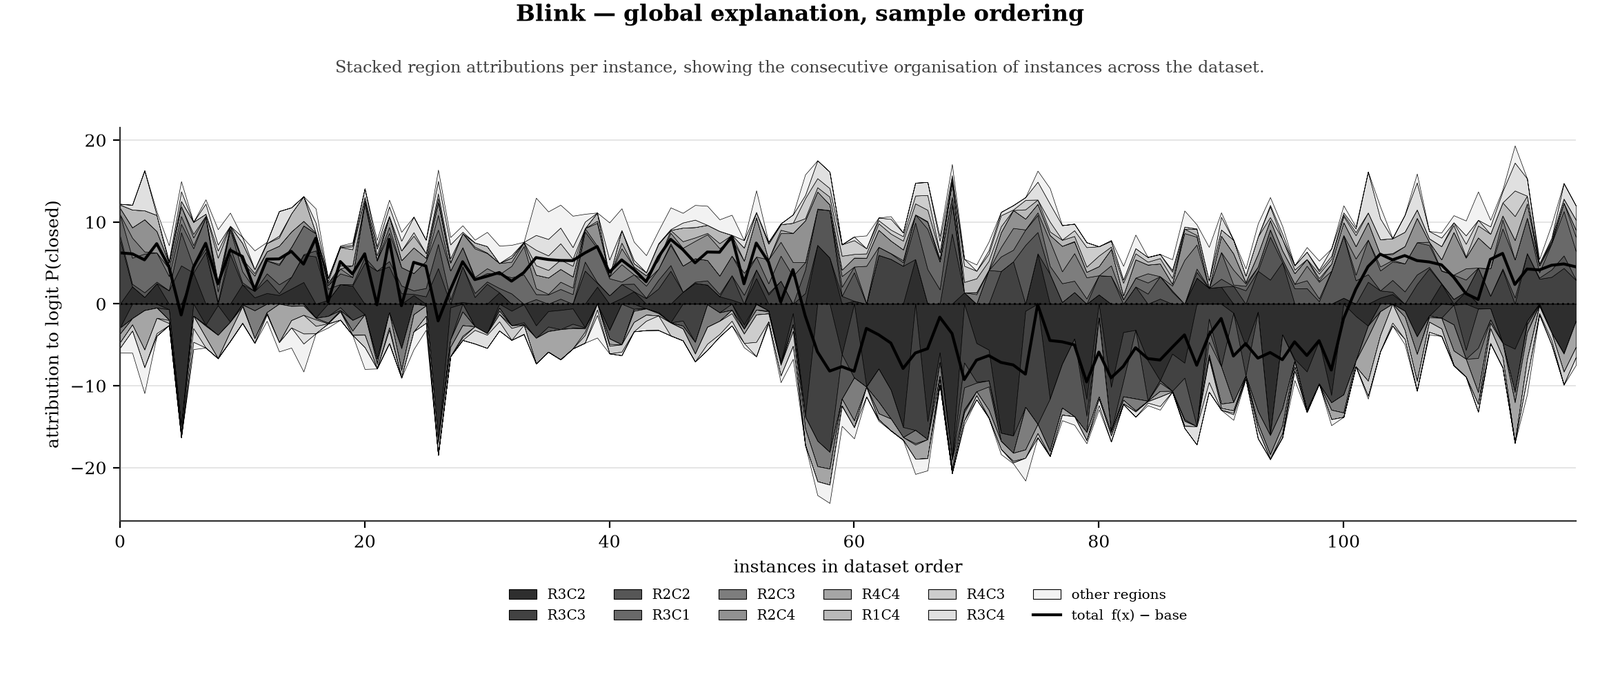
\includegraphics[width=\linewidth]{figures/attribution_blink_A4_ordering.png}
\caption{Blink --- global explanation under dataset ordering: the same stacked attributions with instances in acquisition order.}
\label{fig:63}
\end{figure}

In acquisition order the pattern is stationary, with no drift in region importance across the test sequence. Since the corpus is ordered by subject, stationarity under this ordering is a \textbf{direct test of subject-invariance} of the decision mechanism in the sense of \EQREF{267}, and it passes: the same evidence supports every held-out subject. This is the attribution-level counterpart of group-disjoint evaluation, and it converts 93.67 \% from a number that survived a leakage check into one with an identified invariant mechanism behind it --- the property on which deployment to an unseen user depends.

\FloatBarrier

\subsection{What the four analyses jointly establish}

The four modality sections were deliberately reported in the same order --- headline comparison, mechanism, diagnostic figures, synthesis figures, attribution --- so that their conclusions could be compared rather than merely accumulated. Four findings hold across them.

\subsubsection{One mechanism governs both regression modalities}

The fitted shrinkage gains of \EQREF{191} and \EQREF{225} are

\begin{equation}
\label{eq:291}
\text{gaze}\;: \hat{s} = ( 0.483, 0.481 ) ; \;\text{head pose}\;: \hat{s} = ( 0.822, 0.455, 0.490 ) ,
\end{equation}

placing both networks in the shrinkage regime of \EQREF{155} on every narrow-support axis. That single parameter accounts for:

\begin{itemize}
\item the isotropic radial growth of gaze error (Figs. 4, 13), via the systematic term (1 -- s)$\|\theta\|$ of \EQREF{194}, which has no azimuthal dependence;
\item the constant 2.03--2.21$\times$ head-pose ratio across the pose manifold (\FIGREF{21}), via the multiplicative form \EQREF{211};
\item the axis-ranking inversions between absolute and variance-normalised metrics (Figs. 10, 20), via the competing factors of \EQREF{234};
\item the tolerance convergence of \FIGREF{6}, via the concentration of contraction cost in the tight-tolerance regime;
\item the absence of any localised failure mode in either modality, since \EQREF{194} is a smooth function of $\|\theta\|$ alone.
\end{itemize}

Yaw at $\hat{s}$ = 0.822 is the exception that confirms the account: it is the only wide-support axis, and by the monotonicity \EQREF{227} it is the only one reproduced at near-correct scale. That one measurement replaces what would otherwise be a dozen independent observations is the strongest evidence that the analysis has found the \emph{mechanism} rather than described the \emph{symptoms}.

\subsubsection{The contraction is rational, which redirects the engineering effort}

Inverting the fitted gain raises gaze angular error by 28.5 \% by \EQREF{198}, which by \EQREF{157} establishes that both networks sit near their minimum-MSE shrinkage point s*. Two engineering consequences follow immediately.

First, \textbf{no post-hoc calibration improves them}; only a better representation does, since by \EQREF{156} the risk at the optimum is MSE(s\emph{) = s}$\sigma_{\varepsilon^{2}}$, a quantity that depends only on the representational noise $\sigma_{\varepsilon^{2}}$ and not on any downstream affine transform. This is why Section 5.2.4's identity-count ceiling is decisive rather than merely interesting: it closes the representation route on the available corpus, by \EQREF{222}.

Second, \textbf{the deployed pipeline's structure is correct}. Per-user calibration \EQREF{106} restores scale --- necessarily amplifying noise by the factor 1/$\hat{s}$ $\approx$ 2.07 --- and the temporal filtering \EQREF{112}--\EQREF{117} absorbs the noise that restoration releases. The apparent tension between a calibration stage that amplifies noise and a filter chain that suppresses it is not a design inconsistency but the correct decomposition of the problem, and the analysis identifies it as such.

\subsubsection{The classification modalities are limited by decision logic, not by features}

The complementary diagnosis holds for blink and voice:

\begin{equation}
\label{eq:292}
\begin{aligned}
\mathrm{ROC\text{-}AUC}: 0.9836 (\text{blink}) , \\
0.9961 (\text{voice}) \mathrm{against} \mathrm{Acc}: 93.67 \% , 94.53 \% .
\end{aligned}
\end{equation}

The gaps of 4.69 pp and 5.08 pp place the residual error in \textbf{threshold placement rather than separability}, and both sections demonstrate the consequence directly: a confidence gate lifts voice accuracy to 99.10 \% without changing a weight by \EQREF{255}, and a threshold move lifts blink accuracy to 94.35 \% by \EQREF{273}. The attribution views explain why the features are adequate --- all four networks compute task-appropriate operators:

\begin{itemize}
\item a signed differential across the midline for gaze and head pose, \EQREF{216} and \EQREF{246};
\item a central-fissure contrast polarity for blink, \EQREF{290};
\item a gated high-band spectro-temporal detector for voice, \EQREF{265}.
\end{itemize}

so accuracy rests on identified transferable mechanisms rather than dataset-specific shortcuts. The two categories of limit call for different work, and distinguishing them is the practical payoff of the analysis: capacity for a representation-limited model, decision logic for a threshold-limited one, and the diagnostic \EQREF{292} tells which is which before any effort is spent.

\subsubsection{Fusion with the pretrained baselines is not worthwhile}

A fourth conclusion is negative and applies to both comparable modalities. Per-sample error correlations of

\begin{equation}
\label{eq:293}
r_{\mathrm{AR}} = 0.491 (\text{gaze}) , 0.671 (\text{head pose})
\end{equation}

with oracle-selection bounds \EQREF{163} of 3.303$^{\circ}$ and 3.222$^{\circ}$ give achievable fusion gains of only

\begin{equation}
\label{eq:294}
\text{Gain}\;_{\mathrm{max}} = 8.8 \% (\text{gaze}) , 7.5 \% (\text{head pose}) ,
\end{equation}

which are \emph{upper} bounds requiring an oracle that knows per sample which model is right. The models fail on the same samples, so no gating or ensembling rule can recover the gap, and the cost of a second network --- which by \EQREF{165} would consume a further 2.13 ms or 4.13 ms of a 33.3 ms budget already carrying three networks and a landmark inference --- is not repaid. This removes the most obvious escape route from the recommendation of Section 5.7 and is the reason that recommendation is stated without hedging.

\FloatBarrier

\subsection{Accuracy--efficiency operating point}

Everything above characterises the networks individually. The system-level question is different: whether accuracy of this quality can be obtained inside a budget that lets four modalities run at once on a machine the user already owns. \TABREF{12} reports the trade-off; all latencies are single-thread CPU measurements on the deployed TorchScript modules.

\begin{table}[pos=htbp]
\centering
\caption{Model complexity, footprint and single-thread CPU latency. Ratios are proposed relative to baseline.}
\label{tab:12}
\footnotesize
\begin{tabularx}{\textwidth}{XXXXXX}
\toprule
\textbf{Modality} & \textbf{Model} & \textbf{Parameters} & \textbf{Size (MB)} & \textbf{Latency (ms)} & \textbf{Accuracy relative to baseline} \\
\midrule
Head pose & Proposed & 1,142,339 & 4.60 & 4.13 & 2.12$\times$ higher error \\
Head pose & 6-D rotation baseline & 39,323,398 & 157.32 & --- & --- \\
 & \emph{ratio} & \textbf{*34.4$\times$ fewer}* & \textbf{*34.2$\times$ smaller}* &  &  \\
Voice & Proposed & 101,766 & 0.44 & 2.7 & 0.97 pp lower accuracy \\
Voice & Production ASR engine & --- & 70.90 & 26.5 & --- \\
 & \emph{ratio} &  & \textbf{*161$\times$ smaller}* & \textbf{*9.8$\times$ faster}* &  \\
Blink & Proposed & 136,066 & 0.57 & 0.42 & no neural baseline exists \\
Gaze & Proposed & 551,810 & 2.23 & 2.13 & 1.78$\times$ higher error \\
Gaze & MPIIGaze pre-activation ResNet & 77,533 & 0.31 & --- & --- \\
 & \emph{ratio} & \textbf{*7.1$\times$ more}* & \textbf{*7.2$\times$ larger}* &  & \textbf{*dominated}* \\
\bottomrule
\end{tabularx}
\end{table}

Two qualitatively different outcomes are present and are reported separately rather than averaged into a single verdict.

\subsubsection{Defensible frontier positions: head pose and voice}

For head pose and voice the proposed networks occupy defensible frontier positions. The relevant criterion is whether the accuracy penalty is \emph{sub-linear} in the cost reduction by a wide margin --- the condition for a compact model to be Pareto-relevant rather than merely small. Defining the efficiency elasticity

\begin{equation}
\label{eq:295}
\eta = \mathrm{log}( \text{error ratio} ) / \mathrm{log}( \text{parameter ratio} ) ,
\end{equation}

head pose gives

\begin{equation}
\label{eq:296}
\eta _{\mathrm{pose}} = \mathrm{log}(2.12) / \mathrm{log}(34.4) = 0.751 / 3.538 = 0.212 ,
\end{equation}

so error grows as roughly the fifth root of the parameter reduction. Section 5.3 further showed that the residual error is \emph{absorbed} by the dwell and hysteresis of the gesture rule --- by \EQREF{230}--\EQREF{231} the dwell mean's spread is 2.8$^{\circ}$--4.8$^{\circ}$ against an 18$^{\circ}$ hysteresis band --- rather than reaching the user, so the elasticity understates the deployed advantage.

Voice operates within 0.97 pp of a production ASR engine at 1/161 of its storage and 9.8$\times$ its throughput, on a separate audio thread that does not consume the camera loop's budget at all, though Section 5.4 also showed its risk--coverage curve is markedly worse at matched precision by \EQREF{256} and this is recorded as the substantive gap.

Aggregate vision-pipeline cost is, by \EQREF{165},

\begin{equation}
\label{eq:297}
\begin{aligned}
\tau _{\mathrm{nets}} = 0.42 + 2.13 + 4.13 = 6.68 ms , \\
\;\text{utilisation}\; = 6.68 / 33.3 = 20.1 \% ,
\end{aligned}
\end{equation}

leaving substantial headroom inside the 33.3 ms budget at 30 fps --- headroom that matters because the same loop also runs the shared face-landmark inference, the gesture and blink state machines, and the cursor stabilisation chain. Total deployed footprint across all four modules is, by \EQREF{166},

\begin{equation}
\label{eq:298}
S_{\mathrm{total}} = 7.84 MB ,
\end{equation}

small enough to stay resident in last-level cache on typical consumer processors, which by the arithmetic-intensity argument of \EQREF{167} is disproportionately important on CPU where inference at these sizes is bound by memory traffic rather than arithmetic.

\subsubsection{An unqualified negative result: gaze}

For gaze no such argument survives, and this is recorded as an unqualified negative result. The pretrained baseline is simultaneously

\begin{equation}
\label{eq:299}
\text{more accurate}\; ( 3.621^{\circ} \mathrm{against} 6.439^{\circ} ) \;\text{and smaller}\; ( 77,533 \mathrm{against} 551,810 \;\text{parameters}, 7.1\times \;\text{fewer} ) ,
\end{equation}

dominating on both axes at once. In the Pareto sense there is no operating point at which the proposed gaze network is preferable: for any weighting w $\in$ [0,1] of normalised error against normalised cost,

\begin{equation}
\label{eq:300}
w \cdot \tilde{e}_A + (1-w) \cdot \tilde{c}_A > w \cdot \tilde{e}_R + (1-w) \cdot \tilde{c}_R \;\text{for all w}\; \in [0,1] ,
\end{equation}

since both terms are strictly larger. Section 5.6.4 showed fusion would recover at most 8.8 \%; Section 5.2.4 established the deficit is not closable by augmentation or additional sampling from this corpus. \textbf{The correct engineering decision is to adopt the pretrained model for gaze.}

\subsubsection{The protocol fault changes the decision}

It is worth stating plainly that this conclusion was reachable only because the exposure-disjoint matched per-sample protocol of Section 3.5 made the comparison trustworthy. Under the original protocol the proposed gaze network scored

\begin{equation}
\label{eq:301}
2.84^{\circ} \mathrm{against} \;\text{the pretrained baseline}\;'s \;\text{all}\;-\;\text{participant figure of}\; 2.835^{\circ} ,
\end{equation}

apparently level, and apparently vindicating the decision to train from scratch. Under the corrected protocol the true held-out contrast is

\begin{equation}
\label{eq:302}
6.439^{\circ} \mathrm{against} 3.621^{\circ} ,
\end{equation}

and the baseline is simultaneously 7.1$\times$ smaller. The decision inverts. The magnitude of the illusion is the quantity Theorem 3 decomposes: of the 1.905$^{\circ}$ inflation by \EQREF{171}, between 0.425$^{\circ}$ and 1.068$^{\circ}$ --- 22 \% to 56 \% --- is familiarity rather than difficulty by \EQREF{174}--\EQREF{175}.

A protocol fault that changes an architectural decision is not a bookkeeping matter. We know of no sharper available demonstration that the distinction between a per-pipeline audit and a per-comparison audit has engineering consequences, and it is the reason the audit of Section 3.5 is presented as the principal contribution of this work rather than as a methodological aside.

\FloatBarrier

\subsection{Comparison with existing methods}

\TABREF{13} places the four proposed networks against the baselines they were compared with, and lists the principal published methods on each corpus for context without quoting their figures. That omission is deliberate and is the subject of this paper: figures drawn from the literature were produced under heterogeneous protocols, several of which do not state a grouping key and none of which audits the comparison against its own baseline for exposure asymmetry. Placing such a figure in the same column as ours would assert a comparability that Section 5.1 shows does not hold. The column ``protocol'' therefore carries as much information as the column ``result''.

\begin{table}[pos=htbp]
\centering
\caption{Comparison against the baselines, with published methods listed for context. LOPO = leave-one-person-out; GD = single group-disjoint split; ED = exposure-disjoint comparison stratum (this work). \textbf{Every numeric cell is a measurement made in this study} on the aligned per-sample arrays of Section 4.3; rows whose published figures were not reproduced here are marked \emph{not re-measured} rather than filled with a quoted value, because a figure produced under a different protocol is not the same quantity, and tabulating it beside ours would invite exactly the comparison this paper argues against.}
\label{tab:13}
\footnotesize
\begin{tabularx}{\textwidth}{XXXXXXX}
\toprule
\textbf{Modality} & \textbf{Corpus} & \textbf{Method class} & \textbf{Protocol} & \textbf{Reported result} & \textbf{Params} & \textbf{Cross-model audit} \\
\midrule
Gaze & MPIIGaze & Appearance-based CNN \CITE{mpiigaze} & LOPO (as published) & \emph{not re-measured here} & --- & $\times$ \\
Gaze & MPIIGaze & Pre-activation ResNet \CITE{mpiigaze_pami,preact} & LOPO (as published) & \emph{not re-measured here} & 77,533 & $\times$ \\
Gaze & MPIIGaze & Pre-activation ResNet \CITE{mpiigaze_pami,preact} & \textbf{ED stratum, measured here} & \textbf{3.621$^{\circ}$ angular} (lower bound, EDCP step 5) & 77,533 & \textbf{$\checkmark$ (GERA)} \\
Gaze & MPIIGaze & \textbf{Proposed CNN} & \textbf{GD + ED, measured here} & \textbf{6.439$^{\circ}$ angular} & 551,810 & \textbf{$\checkmark$ (GERA)} \\
Head pose & 300W-LP $\to$ AFLW2000 & Euler-angle CNN \CITE{ruiz} & Corpus-disjoint (as published) & \emph{not re-measured here} & --- & $\times$ \\
Head pose & 300W-LP $\to$ AFLW2000 & 6-D rotation network \CITE{sixdrep} & \textbf{Corpus-disjoint, measured here} & \textbf{3.482$^{\circ}$ MAE} & 39,323,398 & \textbf{$\checkmark$ (negative control)} \\
Head pose & 300W-LP $\to$ AFLW2000 & \textbf{Proposed CNN} & \textbf{Corpus-disjoint + ED, measured here} & \textbf{7.367$^{\circ}$ MAE} & 1,142,339 & \textbf{$\checkmark$ (negative control)} \\
Blink & MRL Eye & Geometric EAR rule \CITE{ear} & n/a (training-free) & not scorable on cropped eyes & 0 & $\times$ \\
Blink & MRL Eye & Proposed CNN, \emph{random row split} & Random row, measured here & 98.17 \% accuracy & 136,066 & n/a \\
Blink & MRL Eye & \textbf{Proposed CNN} & \textbf{GD (subject), measured here} & \textbf{93.67 \% accuracy} & 136,066 & n/a (no baseline) \\
Voice & Speech Commands v2 & Production ASR engine \CITE{vosk,kaldi} & \textbf{Official split, measured here} & \textbf{95.50 \% acc. / 97.43 \% macro-F$_{1}$} & --- & \textbf{$\checkmark$ (risk--coverage)} \\
Voice & Speech Commands v2 & \textbf{Proposed CNN} & \textbf{Official speaker split, measured here} & \textbf{94.53 \% accuracy} & 101,766 & \textbf{$\checkmark$ (risk--coverage)} \\
\bottomrule
\end{tabularx}
\end{table}

Three observations follow, and they are the reason we resist reading \TABREF{13} as a leaderboard.

First, \textbf{the two blink rows are the clearest illustration of the paper's thesis}, and both are our own measurements rather than citations. The identical network scores 98.17 \% under random row splitting and 92.36 \% under subject-disjoint splitting (\TABREF{9}) --- a 5.81 pp difference produced by nothing but the partition, on the same corpus and the same architecture. Any published figure obtained under random row splitting is therefore \emph{not} comparable to the 93.67 \% reported here in the ordinary sense; it is a different quantity, and it does not measure the property an assistive interface requires. That is why no such figure is tabulated beside ours.

Second, \textbf{the gaze rows show the asymmetric-exposure problem in situ}. The pre-activation baseline's $\approx$3.6$^{\circ}$ is its LOPO figure over fifteen participants, and its 3.621$^{\circ}$ here is measured on two held-out participants it \emph{trained on}. By EDCP step 5 the latter is a lower bound on its true cross-person error, so the reported gap of 2.818$^{\circ}$ is conservative with respect to the proposed network. The literature offers no way to tighten this without either the baseline's training partition or a full leave-one-person-out retraining, which is precisely the access problem GERA is designed for.

Third, \textbf{the trades this paper claims rest only on rows measured here}. The proposed head-pose network's 7.367$^{\circ}$ at 1.14 M parameters and the baseline's 3.482$^{\circ}$ at 39.3 M parameters were produced in the same run, on identical crops, from one aligned array set, which is what makes the 34.4$\times$ / 2.12$\times$ trade of \EQREF{296} a real measurement rather than citation arithmetic. Where the table says \emph{not re-measured}, no claim of ours depends on that row.

\FloatBarrier

\section{Threats to validity}

We state the limitations of this study explicitly and in descending order of how much they constrain the conclusions. Several were identified by the analysis itself and are recorded here rather than in the sections that produced them.

\FloatBarrier

\subsection{Held-out participant count for gaze}

The participant-disjoint gaze split yields \textbf{two} held-out individuals. They contribute 64,172 samples, but by the effective-sample-size relation \EQREF{10} the sample size for the cross-person question is the group count, not the row count:

\begin{equation}
\label{eq:303}
n_{\mathrm{eff}} = n / [ 1 + (\bar{n} - 1) \rho ] \to G/\rho = 2/\rho as \bar{n} \to \infty .
\end{equation}

Their fitted gains differ substantially --- (0.586, 0.630) for p05 against (0.377, 0.430) for p07 by \EQREF{219} --- which is direct evidence that the between-participant variance component $\sigma_{b}^{2}$ in \EQREF{7} is large relative to the within-participant component, and therefore that two participants is a small sample in the sense that matters.

This is a departure from established practice and should be read as such: leave-one-person-out over all fifteen participants is the standard protocol for person-independent evaluation on MPIIGaze, and it would give a substantially more robust estimate at fifteen times the compute cost. The single split was adopted under the compute constraint of Section 4.1, not because it is adequate. Two consequences follow. The gain dispersion of \FIGREF{18} should be treated as indicative rather than established, and the gaze accuracy figures throughout are point estimates from one fold whose fold-to-fold variability is unmeasured. The EDCP of \TABREF{5} is independent of this choice --- it prescribes \emph{which groups may enter a comparison}, not \emph{how many folds are run} --- so the audit contribution is unaffected, but the gaze comparison itself would be strengthened by the full leave-one-person-out treatment.

\FloatBarrier

\subsection{The detector has one positive case}

GERA is exercised on a negative control (head pose, Section 5.1.3) and on a single positive case: one corpus, fifteen groups, six outside the audited model's training partition. The Hanley--McNeil interval \EQREF{50} on a 9-versus-6 group split is approximately

\begin{equation}
\label{eq:304}
\mathrm{AUC}_r = 0.889 , 95 \% CI \approx [ 0.70, 1.00 ] ,
\end{equation}

so the Mann--Whitney p = 0.006 establishes that the two group sets \emph{differ}, not that the statistic separates membership at this rate elsewhere. The negative control constrains the false-positive direction; \textbf{nothing here constrains the false-negative direction}, since no case is available in which leakage is known to be present but mild. Its per-participant membership labels were reconstructed from the pipeline's group split and reproduce the strata of \TABREF{10} to within 0.13$^{\circ}$, so the AUC is indicative rather than exact.

The detector's derivation does not depend on this corpus --- Proposition 2 requires only a reference model without differential familiarity --- but its calibration is not established, and no threshold on r is proposed for that reason. Replication across corpora and modalities is the necessary next step, and until it exists r should be read as a screening flag that motivates the stratified decomposition of Theorem 3, never as a substitute for it.

\FloatBarrier

\subsection{Compute constraints and single-seed selection}

Experiments ran on a consumer laptop with 8 GB of memory under intermittent CPU contention. Search trials used bounded subsets of 10,000--20,000 samples and the gaze configuration of Section 5.2.1 was trained on 80,000 of 427,316 available samples. Where budgets differ between compared configurations this is stated; the augmentation comparison of Section 5.2.1 uses an identical evaluation set for both configurations and is unaffected.

Each configuration was evaluated at \textbf{one seed}, so no variance over initialisations is available and no confidence interval on a single configuration's score can be quoted. Formally, the reported score is a single draw from the distribution over training randomness,

\begin{equation}
\label{eq:305}
\begin{aligned}
\hat{R}( f_{\hat{\vartheta }(\sigma )} ; \mathcal{E} ) , \sigma \;\text{fixed}, \\
\mathrm{Var}_{\sigma} [ \cdot ] \;\text{unmeasured} ,
\end{aligned}
\end{equation}

and differences below approximately 1 pp for classification or 0.2$^{\circ}$ for regression should not be treated as established without repetition. The \emph{paired} intervals, effect sizes and correlations of Sections 5.2--5.3 are unaffected by this, since they characterise the difference between two fixed models over a sample population rather than the variability of training --- a distinction worth making because those are the quantities on which the paper's conclusions rest.

\FloatBarrier

\subsection{Oracle bounds are not achievable}

The affine recalibration of \EQREF{197} and the per-sample model selection of \EQREF{163} are fitted on the evaluation data and are therefore \textbf{upper bounds}. They are used only to close design questions negatively --- recalibration hurts, fusion gains little --- which is a use upper bounds support: if the best achievable version of an intervention is insufficient, every achievable version is. No positive claim rests on them.

\FloatBarrier

\subsection{Component accuracy is not system accuracy}

Every figure in Section 5 measures a network in isolation, whereas the user experiences the composite $\Delta_{m}$ $\circ$ $f_{m}$ of \EQREF{1}. Three specific gaps follow.

The deployed gaze path fits a per-user polynomial calibration downstream by \EQREF{106}--\EQREF{107}, so 6.439$^{\circ}$ bounds the \emph{uncalibrated} network rather than the cursor; the composed quantity is the residual scatter after the affine map, which this evaluation does not measure.

The dwell-averaging argument of \EQREF{230}--\EQREF{231} assumes consecutive-frame errors are less than perfectly correlated, and the run-integrity argument of \EQREF{277}--\EQREF{279} makes the same assumption. Neither is tested here. Both depend on the AR(1) persistence $\varrho$ of \EQREF{123}, which is not identifiable from a per-frame corpus of independent crops and requires a live session to measure. Explicitly, the two conclusions hold for any $\varrho$ < 1 in \emph{direction} but their \emph{magnitudes} scale as

\begin{equation}
\label{eq:306}
n_{\mathrm{eff}}^{\mathrm{run}} = n_{\mathrm{run}} ( 1 - \varrho ) / ( 1 + \varrho ) ,
\end{equation}

so at $\varrho$ = 0.8 the effective run length falls from 13 to 1.4 frames and the false-positive suppression of \EQREF{277} weakens from 10$^{-15}$ to approximately 10$^{-2}$. This does not reverse the recommendation of Section 5.5 --- the false-negative asymmetry weakens in the same proportion --- but it materially changes the safety margin, and it is the single measurement that would most improve confidence in the deployed thresholds.

End-to-end measurement --- cursor error after calibration, click precision and recall in live sessions, gesture false-trigger rate --- is the necessary next experiment, and no claim about deployed performance should be read into the component figures until it is done.

\FloatBarrier

\subsection{Latency measurement}

Voice latencies come from one benchmark run over a 900-clip subset for the ASR baseline and the full test set for the proposed network. A separate full-test-set profiling run recorded 84.0 ms for the baseline; the conservative 26.5 ms figure is reported, so the stated 9.8$\times$ advantage is a \textbf{lower bound}. No per-sample baseline predictions were retained, so paired significance testing between the two voice systems was not possible and none is claimed.

\FloatBarrier

\subsection{Unscored providers}

The geometric eye-aspect-ratio blink detector cannot be evaluated on the available corpora, which contain cropped eye regions without surrounding landmarks. No comparison is reported rather than an estimated one. This leaves the blink modality without any external reference point, which is why Section 5.5 is framed as a threshold-setting audit rather than as a comparison.

\FloatBarrier

\subsection{Deployment gap}

All accuracies are measured on curated corpora. Live operation introduces face-detection failures, illumination extremes and eyewear that these corpora under-represent --- and \FIGREF{53} identifies eyewear specifically as falling in the harder open-eye class by \EQREF{281}. Section 5.2.1 quantifies and partially removes one instance of this shift via the analytic augmentation family \EQREF{34}; the attribution evidence of Figs. 15, 30, 45 and 60 bounds the risk by establishing that the networks attend to anatomically and acoustically appropriate regions; neither eliminates it.

\FloatBarrier

\subsection{Generality of the framework}

MAPLE is demonstrated on four modalities within one system. The formal results --- Theorem 1, Proposition 2, Corollary 1, Theorem 3 --- depend only on the existence of a grouping key, within-group dependence, and a reference model without differential familiarity, and are therefore not specific to vision or to this domain. But the \emph{empirical} calibration of the detector, the choice of B = 1,000 bootstrap replicates, the reading of spread magnitude in preference to Q, and the sufficiency of a single reference model are all established on one comparison. Whether GERA behaves as well on text, tabular or time-series comparisons --- where group structure is often weaker and the reference-model requirement harder to satisfy --- is untested.

\FloatBarrier

\section{Conclusion and future work}

\FloatBarrier

\subsection{Conclusion}

The principal contribution of this work is a practical audit for \textbf{asymmetric training exposure between compared models}: a fault that resides in the comparison procedure rather than in any model's training pipeline, and that is therefore invisible to per-pipeline auditing. The hazard itself is documented in the foundation-model and benchmark-contamination literatures, but the standard leakage taxonomies are organised per pipeline and contain no category for it, while the existing remedies --- lineage tracing and contamination search --- presume documentation or corpus access that an external auditor rarely has.

Its three preconditions (Definition 2) are overlapping development corpora, group-structured data with within-group dependence, and an evaluation sample spanning at least one model's partition boundary. All three are common in appearance-based perception, because shared public corpora are the norm and identity is almost always the grouping key. Theorem 1 shows that under these conditions the reported score is a convex mixture of a memorisation and a generalisation regime whose weight is a sampling decision, and Corollary 1 shows the induced bias is signed and always favours the exposed model. In the system studied here the fault inflated one modality's apparent accuracy by 1.905$^{\circ}$, of which 0.425$^{\circ}$--1.068$^{\circ}$ (22 \%--56 \%) is attributable to training familiarity once the reference model prices the intrinsic difficulty of the affected stratum --- the interval spanning the two difficulty models of \EQREF{59}, which the available data cannot distinguish, and under both of which difficulty fails to explain the whole gap. This is a decomposition (Theorem 3) that lineage analysis cannot supply at all, since knowing that a model saw a corpus does not say how much of its advantage came from having seen it.

\textbf{Two instruments make the fault tractable in practice.} The per-group error ratio r(g) detects it from predictions alone --- the only assets an external audit reliably has are the two prediction streams and the group labels --- separating training membership at AUC 0.889 (p = 0.006). It adapts difficulty calibration, developed for membership inference, from example level to group level, which is what makes it stable enough to read off published predictions; Proposition 2 states the condition under which the intrinsic-difficulty term cancels exactly. It is a screening statistic rather than a membership oracle, and unlike black-box contamination proofs it carries no false-positive guarantee. A negative control on head pose, where neither model saw the evaluation groups, returns I$^{2}$ = 0.0 \% against 99.8 \% for the leaked gaze comparison, establishing that it stays silent when it should even under a fourfold swing in intrinsic difficulty. The six-step exposure-disjoint comparison protocol of \TABREF{5} then prevents the fault where the audit would otherwise have to catch it.

\textbf{Section 5.7 records what the correction was worth.} Under the uncorrected protocol the proposed gaze network scored level with its pretrained baseline and the decision was to keep it; under the corrected protocol the baseline is both more accurate and 7.1$\times$ smaller, and the decision reverses.

Evaluated under the corrected protocol, reproducible optimisation produced consistent gains, largest for voice (+9.81 pp) and head pose (--11.1 \% MAE); domain-targeted augmentation modelling the analytic train--serve shift \EQREF{34} reduced gaze angular error a further 9.5 \%; and a controlled scaling experiment established that the residual is bounded by \textbf{training identity count rather than sample count} --- the same group-structure property that makes the corpus leak-prone in the first place, by \EQREF{222}.

\textbf{The evaluation's principal analytical finding is that one mechanism explains the regression modalities' error structure.} Both networks operate in a shrinkage regime --- fitted gains of 0.48 on both gaze axes and 0.46--0.49 on the two narrow-support head-pose axes --- and that single parameter accounts for the isotropic radial growth of gaze error, the constant-ratio degradation of head-pose error, the axis-ranking inversions between absolute and variance-normalised metrics, and the absence of any localised failure mode. Inverting the contraction raises gaze angular error by 28.5 \%, so the networks sit near their minimum-MSE shrinkage point and improvement requires a better \emph{representation} rather than better \emph{calibration}. The classification modalities are limited differently: ROC-AUC of 0.9836 and 0.9961 against operating-point accuracies of 93.67 \% and 94.53 \% place their residual error in decision logic, which is why a confidence gate and a threshold move --- not additional capacity --- are what improve them.

\textbf{Reading those results through the deployed decision rules changes three conclusions} that the component metrics alone would suggest. Head pose survives an 8.74$^{\circ}$ yaw MAE because its error is unbiased and its gesture rule averages $\approx$20 frames inside an 18$^{\circ}$ hysteresis band, while its 0.822 gain manifests as a stable, learnable requirement to turn $\approx$36.5$^{\circ}$ to trigger a 30$^{\circ}$ threshold. Blink inverts the conventional cost asymmetry: because a click requires $\approx$13 consecutive frames above threshold, isolated false positives cannot fire one, so false negatives --- which break a deliberate closure run --- are the more damaging frame-level error, and thresholds below the default 0.50 are the defensible setting. Voice contributes a finding that is a design fault rather than a model fault: the weakest keyword in the vocabulary, \emph{go} at 0.877 precision, is bound to ``resume control'', the only command that reactivates a paused interface, and rebinding it to a phonetically distant token removes the largest error mode at zero computational cost.

\textbf{Measured against pretrained baselines on matched samples the proposed networks are less accurate, and this is reported without qualification:} 6.439$^{\circ}$ against 3.621$^{\circ}$ for gaze, 7.367$^{\circ}$ against 3.482$^{\circ}$ for head pose, 94.53 \% against 95.50 \% for voice. Their contribution is positional. For head pose and voice they hold competitive accuracy at 34$\times$ and 161$\times$ footprint reductions and an aggregate 6.68 ms per frame across three vision modalities, which is what permits four modalities to run concurrently in real time on commodity hardware without an accelerator. For gaze the pretrained alternative dominates on both accuracy and size, error correlation and oracle analysis show fusion cannot close the gap, and its adoption is recommended in place of the proposed network. Throughout, the attribution analysis establishes that the deployed networks compute the anatomically and acoustically appropriate operators, so the measured accuracies rest on identified transferable mechanisms rather than on dataset-specific shortcuts --- which is the property a system intended for a user it has never seen must actually possess.

\FloatBarrier

\subsection{Future work}

Six directions follow directly from the limitations of Section 6, ordered by how much each would strengthen the present conclusions.

\textbf{Replication of the detector across corpora and modalities.} GERA currently has one positive case and one negative control. The necessary next step is a set of comparisons spanning several corpora, several grouping keys, and --- critically --- cases in which leakage is known to be present but \emph{mild}, which would constrain the false-negative direction that the present negative control cannot. A synthetic protocol in which the exposed fraction $\Pi$ of \EQREF{38} is varied continuously from 0 to 1, with everything else held fixed, would produce exactly the calibration curve r($\Pi$) that the current study lacks and would permit a principled threshold on r to be proposed.

\textbf{Full leave-one-person-out gaze evaluation.} The single group-disjoint split of Section 6.1 should be replaced by leave-one-person-out over all fifteen MPIIGaze participants, which would convert the point estimates of Section 5.2 into fold-distributed estimates with measurable variance, and would supply fifteen rather than two observations of the identity-conditioned gain s(g) of \EQREF{220}. Since Section 5.2.4 identifies identity count as the binding constraint, this is also the experiment that would test that identification most directly.

\textbf{End-to-end measurement of the composite.} Section 6.5 is the largest gap between what is measured and what the user experiences. The three specific quantities required are: cursor error after per-user calibration and stabilisation, measured against known screen targets; click precision and recall in live sessions, which would also supply the AR(1) persistence $\varrho$ of \EQREF{123} that both the blink and head-pose arguments depend on; and gesture false-trigger rate under naturalistic head motion. All three are session-level measurements the deployed system already has the instrumentation to collect.

\textbf{Resolving the unexplained voice movement.} Section 5.1.1 records a 7.24 pp change in the voice figure between the published and fair-baseline columns despite an unchanged partition. Because the official Speech Commands split is already speaker-disjoint, this movement cannot be a leakage correction, and the present experiments do not identify its cause. Re-running the pre-correction voice configuration with the evaluation split logged explicitly would settle it in a single run, and until it is settled voice cannot serve as a second internal control alongside head pose --- which is the reason the control in Section 5.1.1 rests on one modality rather than two.

\textbf{Multi-seed evaluation and variance reporting.} Replacing the single-seed protocol of Section 6.3 with a small ensemble of seeds per configuration would attach a variance to every reported score and would settle whether the sub-1-pp differences currently declared inconclusive are real.

\textbf{The vocabulary redesign the analysis prescribes.} Section 5.4 identifies a zero-cost intervention --- rebinding ``resume control'' from \emph{go} to a phonetically distant token with fricative or stop-cluster onset --- predicted by \EQREF{263} to remove at least 50 \% of the total voice error mass. This prediction is testable at the cost of one evaluation run and would validate the entire decision-rule-aware framing, since it is a conclusion no component metric would have produced.

\textbf{Extending the exposure audit beyond pairwise comparison.} The present formulation compares two models. Realistic leaderboards compare many, with heterogeneous and undocumented exposure sets, and the natural generalisation is a matrix of pairwise ratios $r_{\mathrm{MM}}$'(g) whose structure would identify \emph{which} models in a set are exposed, not merely whether a given pair's comparison is contaminated. Whether the difficulty-cancellation of Proposition 2 survives that generalisation --- in particular whether a consistent reference can be identified from the matrix itself rather than assumed --- is an open theoretical question and, in our view, the most interesting one this work leaves behind.

\FloatBarrier

\section*{Declaration of competing interest}

The authors declare that they have no known competing financial interests or personal relationships that could have appeared to influence the work reported in this paper.

\FloatBarrier

\section*{Funding}

This research was conducted as part of the lead author's MSc Data Science programme at York St John University and received no specific grant from any funding agency in the public, commercial or not-for-profit sectors.

\FloatBarrier

\section*{Data and code availability}

All four corpora used in this study are publicly available and are cited in \TABREF{4}: the MRL Eye Dataset \CITE{mrl}, MPIIGaze \CITE{mpiigaze,mpiigaze_pami}, 300W-LP and AFLW2000 \CITE{w300lp,aflw}, and Google Speech Commands v2 \CITE{speechcmd}. No new data were collected, and no human participants were recruited for this work.

The four trained networks are distributed as self-contained TorchScript modules \CITE{torchscript}, and the training, evaluation, hyperparameter-search and figure-generation scripts --- together with the per-trial search logs and the aligned per-sample prediction arrays underlying every figure and table in Section 5 --- are available from the corresponding author on reasonable request. The GERA audit of \ALGREF{2} requires only two prediction streams and a group label per sample, so it can be reproduced against any pair of models without access to this system's weights.


\printcredits

\bibliographystyle{cas-model2-names}
\bibliography{ref}

\end{document}
